% I begin this version on February 3 2012
% on the base of the lecture course of the previous year
% today 1-st February I am working on the version for 2013 year.
% today 31-sr January I am working on the version for 2014 year.
% today 31-sr January I am working on the version for 2015 year.
\def\vare {\varlepsilon}
% today 4-th February I am working on the version for 2016 year.
% today 24 January I am working on the version for 2017 year.
% It will be essentially changes in the second part.
% today 14 January 2018.
% I am working on the version putting the 
%files on conic sect%ion, and Projective geometry in the text.
% Today 20 january 2017 I began to revise the 
%fist section to make it four lectures shorter????



\def\A {{\bf A}}
\def\c{{\bf c}}
\def\t {\tilde}
\def\a {\alpha}
\def\ac{{\bf a}}
\def\K {{\bf K}}
\def\N {{\bf N}}
\def\V {{\cal V}}
\def\s {{\sigma}}
\def\S {{\Sigma}}
\def\s {{\sigma}}
\def\p{\partial}
\def\pt {{\bf p}}
\def\vare{{\varepsilon}}
\def\Q {{\bf Q}}
\def\D {{\cal D}}
\def\G {{\Gamma}}
\def\C {{\bf C}}
\def\M {{\cal M}}
\def\Z {{\bf Z}}
\def\U  {{\cal U}}
\def\H {{\cal H}}
\def\R  {{\bf R}}
\def\E  {{\bf E}}
\def\l {\lambda}
\def\degree {{\bf {\rm degree}\,\,}}
\def \finish {${\,\,\vrule height1mm depth2mm width 8pt}$}
\def \m {\medskip}
\def\p {\partial}
\def\r {{\bf r}}
\def\v {{\bf v}}
\def\n {{\bf n}}
%\def\t {{\bf t}}
\def\b {{\bf b}}
\def\e{{\bf e}}
\def\f{{\bf f}}
\def\g{{\bf g}}
\def\ac {{\bf a}}
\def \X   {{\bf X}}
\def \Y   {{\bf Y}}
\def \x   {{\bf x}}
\def \y   {{\bf y}}
\def \z   {{\bf z}}
\def \f   {{\bf f}}
\def \l   {{\bf l}}
\def\w{{\omega}}
\def \k   {{\bf \kappa}}
\def\la {\langle}
\def \ra {\rangle}
%\def \( {\langle}
%\def \) {\rangle}
\def\proj {{\rm proj}}



\documentclass[12pt]{article}
\usepackage{amsmath,amsthm}
\usepackage{amsmath,amssymb,amsfonts,amsthm,tikz}
%\theoremstyle{theorem}
%\newtheorem{thm}{Khimera}



\numberwithin{equation}{section}

\title{Introduction to  Geometry}
\date{}
\begin{document}
\maketitle

  \centerline {it is a draft of lecture notes of H.M. Khudaverdian.}

  \centerline { Manchester, 14 February 2019}

\tableofcontents
\pagenumbering{roman}

\newpage
%\setcounter{page}{3}
\pagenumbering{arabic}
\section {Euclidean space}

\subsection{Recollection of vector space and Euclidean vector
space}

We recall here important notions from linear algebra
of vector space and Euclidean vector space.


\subsubsection {Vector space.}


\bigskip

Vector space $V$ on real numbers is a set of 
vectors with operations
$"+"$---addition of vector and 
$"\cdot"$---multiplication of vector
Lon real number (sometimes called coefficients, scalars). 

\m

\footnote{ These
operations obey the following axioms


\begin{itemize}
 \item  $\forall \ac,\b\in V, \ac+\b\in V$,

 \item $\forall \lambda\in \R, \forall \ac\in V, \lambda \ac\in V$.

\item
  $\forall \ac,\b \ac+\b=\b+\ac$  (commutativity)
\item
$\forall \ac,\b,\c, \,\,\ac+(\b+\c)=(\ac+\b)+\c$ (associativity)

\item  $\exists\,\, {\mathbf 0}$ such that $\forall \ac$,
 $\ac+{\mathbf 0}=\ac$

\item  $\forall \ac$ there exists a vector $-\ac$ such that $\ac+(-\ac)=0$.

\item

  $\forall\lambda\in \R, \lambda(\ac+\b)=\lambda \ac+\lambda \b$

  \item

    $\forall\lambda,\mu\in \R (\lambda+\mu)\ac=\lambda\ac+\mu\ac$

    \item $(\lambda\mu)\ac=\lambda(\mu\ac)$

    \item $1\ac=\ac$

\end{itemize}
}

\smallskip

{\bf Remark} We denote by $0$ real number  $0$ and {\it vector }
$\bf 0$. Sometimes we have to be careful to distinguish
between zero  vector $\bf 0$ and number zero.

\smallskip


\subsubsection {Basic example of ($n$-dimensional) vector space---$\R^n$}

 A basic example of vector space (over real numbers) is a space
  of ordered $n$-tuples of real numbers.


\noindent  $\R^2$ is a space of pairs of real numbers. $\R^2=\{(x,y),\,\,x,y\in \R \}$

\noindent    $\R^3$ is a space of triples  of real numbers. $\R^3=\{(x,y,z),\,\,x,y,z\in \R \}$

\noindent    $\R^4$ is a space of quadruples  of real numbers. $\R^4=\{(x,y,z,t),\,\,x,y,z,t,\in \R \}$

  \centerline {and so on...}
  $\R^n$---is a space of $n$-typles of real numbers:
                    \begin{equation}
\label{basisexampleofvectorspace}
         \R^n=\{(x^1,x^2,\dots,x^n),\,\,x^1,\dots,,x^n\in \R \}
                     \end{equation}
  If  $\x,\y\in \R^n$ are two vectors, $\x=(x^1,\dots,x^n)$, $\y=(y^1,\dots,y^n)$
then             $$
        \x+\y=(x_1+y_1,\dots,x_n+y_n)\,.
                 $$ and
multiplication on scalars is defined as
           $$
\lambda\x=\lambda \cdot (x^1,\dots,x^n)=(\lambda x^1,\dots,\lambda x^n)\,,\quad (\lambda\in \R)\,.
           $$





\subsubsection{Linear dependence of vectors}



We often consider linear combinations  in vector space:
           \begin{equation}\label{linearcombination}
            \sum_i\lambda_i\x_i=\lambda_1\x_1+\lambda_2\x_2+\dots+\lambda_m\x_m\,,
           \end{equation}
          where $\lambda_1,\lambda_2,\dots,\lambda_m$ are coefficients (real numbers),
          $\x_1,\x_2,\dots,\x_m$ are vectors from vector space $V$.
We say that linear combination \eqref{linearcombination} is {\it \,trivial\,} if all coefficients $\lambda_1,\lambda_2,\dots,\lambda_m$ are equal to zero.
              $$
               \lambda_1=\lambda_2=\dots=\lambda_m=0\,.
               $$
We say that linear combination \eqref{linearcombination} is {\it not trivial} if at least one of  coefficients $\lambda_1,\lambda_2,\dots,\lambda_m$ is not equal to zero:
                    $$
         \lambda_1\not=0, {\rm or}\lambda_2\not=0,{\rm or}\dots {\rm or} \lambda_m\not=0\,.
                    $$

Recall definition of linearly dependent and linearly independent vectors:

{\bf Definition} The vectors $\{\x_1,\x_2,\dots,\x_m\}$ in vector space $V$ are {\it linearly dependent\,}
if there exists a non-trivial linear combination of these vectors such that it is equal to zero.

In other words we say that the vectors $\{\x_1,\x_2,\dots,\x_m\}$ in vector space $V$ are {\it linearly dependent\,} if there exist
coefficients $\mu_1,\mu_2,\dots,\mu_m$ such that at least one of these coefficients is not equal to zero and
               \begin{equation}\label{defoflindepend}
             \mu_1\x_1+\mu_2\x_2+\dots+\mu_m\x_m=0\,.
                 \end{equation}

Respectively  vectors $\{\x_1,\x_2,\dots,\x_m\}$ are {\it linearly independent\,} if they are not linearly dependent.
  This means that an arbitrary linear combination of these vectors which is equal  zero is trivial.

In other words
vectors $\{\x_1,\x_2,\x_m\}$ are {\it linearly independent} if the condition
                      $$
                      \mu_1\x_1+\mu_2\x_2+\dots+\mu_m\x_m=0
                      $$
implies that $\mu_1=\mu_2=\dots=\mu_m=0$.



Very useful and workable

{\bf Proposition }
{\it Vectors $\{\x_1,\x_2,\dots,\x_m\}$ in vector space $V$ are {\it linearly dependent\,}
if and only if at least one of these vectors is expressed via linear combination of other vectors:}

               \begin{equation*}\label{lineardependant}
             \x_i=\sum_{j\not =i}\lambda_j\x_j\,.
               \end{equation*}


   \subsubsection {Dimension of vector space. 
Basis in vector space.}\label{basis}


{\bf Definition }  Vector space $V$ has a dimension $n$  if 
there exist $n$  linearly independent vectors
in this vector space, and  any $n+1$ vectors in $V$ are  linearly dependent.

{\footnotesize In the
case if in the vector space $V$ for an arbitrary $N$
there exist $N$
linearly independent vectors
then the space $V$ is {\it infinite-dimensional}.
An example of infinite-dimensional vector space is a space $V$
of all polynomials of an arbitrary order. One can see that
for an arbitrary $N$ polynomials
           $\{1,x,x^2,x^3,\dots,x^N\}$
are linearly idependent. (Try to prove it!).
This implies $V$ is infinite-dimensional vector space.
}

\m


% end of the first week. I added also affine spaces.
% 5 February
 
       \centerline {\it Basis}

 {\bf Definition}
 Let $V$ be $n$-dimensional vector space.  
The ordered set $\{\e_1,\e_2,\dots,\e_n\}$
 of $n$  linearly independent vectors in $V$ is called a 
basis of the vector space
 $V$.
\m

{\bf Remark}  We say `a basis', not `the basis' since there
 are many bases in the vector space (see also Homeworks 1.2).

{\bf Remark} Focus your attention: basis is  {\it an ordered} 
set of vectors, not just a set of vectors\footnote
{See later on orientation of vector spaces, where the ordering 
of vectors of basis
will be highly important.}.

The following Proposition is very useful:

 {\bf Proposition }
 {\it Let $\{\e_1,\dots,\e_n\}$ be an arbitrary basis 
in $n$-dimensional vector space $V$.
 Then any vector $\x\in V$ can be expressed as a 
linear combination of vectors
 $\{\e_1,\dots,\e_n\}$ in a unique way, i.e.
  for every vector $\x\in V$ there exists an 
ordered set of coefficients $\{x^1,\dots,a^n\}$ such that
                            \begin{equation}\label{expansionofvector}
      \x=x^1\e_1+\dots+x^n\e_n
                            \end{equation}
 and if

                      \begin{equation}\label{uniquenessofexpansion}
      \x=a^1\e_1+\dots+a^n\e_n=b^1\e_1+\dots+b^n\e_n\,,
                            \end{equation}
 then $a^1=b^1, a^2=b^2,\dots,a^n=b^n$. In other words
for any vector $\x\in V$ there exists an ordered $n$-tuple 
$(x^1,\dots,x^n)$ of coefficients
  such that  $\x=\sum_{i=1}^nx^i\e_i$  and this 
$n$-tuple is unique.}

%\end{document} % 31 January

\m

In other words:

 {\bf Basis is a set of  linearly independent
 vectors in vector space $V$ which span (generate) vector space   $V$.}

Recall that we say that vector space $V$  is 
{\it spanned} by vectors $\{\x_1,\dots,\x_n\}$
(or vectors vectors $\{\x_1,\dots,\x_n\}$ 
{\it span} vector space $V$ ) if any vector $\ac\in V$
can be expresses as a linear combination of 
vectors $\{\x_1,\dots,\x_n\}$.


\m

 {\bf Definition}
 Coefficients $\{a^1,\dots,a^n\}$ are called 
{\it components of the vector $\x$ in the 
basis $\{\e_1,\dots,\e_n\}$}
 or just shortly {\it components of the vector $\x$}.

 \m
%\end{document}



{\bf Example} {\it Canonical basis  in $\R^n$}

\m


We considered above  the basic example of 
vector space---a space
of ordered $n$-tuples of real numbers: 
$\R^n=\{(x^1,x^2,\dots,x^n),  x^i\in \R\}$
(see \eqref{basisexampleofvectorspace}).
 One can see that it is $n$-dimensional vector space.
Consider vectors $\e_1,\e_2,\dots,\e_n\in \R^n$:
                  \begin{equation}\label{basicvectors}
                  \begin{array}{cc}
                    \e_1=& (1,0,0\dots,0,0) \\
                    \e_2=& (0,1,0\dots,0,0) \\
                    \dots & \dots \\
                    \e_n=& (0,0,0\dots,0,1) \\
                  \end{array}
                  \end{equation}
Then for an arbitrary vector   
$\R^n\ni \ac=(a^1,a^2,a^3,\dots,a^n)$,
                      $$
               \ac=
    a^1(1,0,0\dots,0,0)+a^2(0,1,0\dots,0,0)+
            a^3(0,0,1,0\dots,0,0)+\dots+a^n(0,1,0\dots,0,1)=
                         $$
                         $$
 \sum_{i=1}^m a^i\e_i=a^i\e_i \qquad \hbox{(we will use sometimes condensed notations}\,\, \x= x^i\e_i)
                            $$


For every vector $\ac\in \R^n$ we have 
unique expansion via the vectors
 \eqref{basicvectors}.
The set of vectors $\{\e_1,\dots,\e_n\}$ 
is a basis of $\R^n$.
 The basis \eqref{basicvectors} is the distinguished basis. 
Sometimes it is called {\it canonical basis in $\R^n$.}
One can find
  another basis in $\R^n$--just take an arbitrary 
ordered set of $n$  linearly independent vectors.
 (See exercises in  Homework 0).




%\end{document} % 31 January 2015
%\end{document} 2    February 2017

\subsubsection {Scalar product. Euclidean space}

In vector space one have additional structure: {\it scalar product of vectors}.

{\bf Definition} Scalar product in a vector space $V$ is  a function $B(\x,\y)$ on a pair of
 vectors which takes real values and satisfies the  the following conditions:
               \begin{equation}\label{scalarproductproperties}
              \begin{array}  {cc}
                B(\x,\y)=B(\y,\x) \quad \hbox  {(symmetricity condition)}\\
                   B(\lambda\x+\mu\x',\y)=
                   \lambda B(\x,\y)+\mu B(\x',\y)\quad   \hbox  {(linearity condition)}\\
                 B( \x,\x)\geq 0\,\, , B(\x,\x)= 0\Leftrightarrow  \x=0\,\,
                 \hbox{(positive-definiteness condition)}
                   \end{array}
               \end{equation}
{\bf Definition } Euclidean space is a vector space equipped with a scalar product.

\m


  One can easy to see that the function $B(\x,\y)$ is bilinear function, i.e.
  it is linear function with respect to the second 
argument also.
  This follows from previous axioms:
                   $$
   B(\x,\lambda\y+\mu\y')\underbrace{=}_{\hbox {symm.}}B(\lambda\y+\mu\y',\x)
   \underbrace{=}_{\hbox {linear. }}\lambda B(\y,\x)+\mu B(\y',\x)
   \underbrace{=}_{\hbox {symm. }}\lambda B(\x,\y)+\mu B(\x,\y')\,.
                   $$

{\footnotesize A bilinear function  $B(\x,\y)$ on pair of vectors is called sometimes {\it bilinear form} on
vector space. Bilinear form $B(\x,\y)$  which satisfies the symmetricity condition is called
{\it symmetric bilinear form}.  Scalar product is nothing but symmetric bilinear form on vectors
which is positive-definite: $B(\x,\x)\geq 0$) and is non-degenerate ($(\x,\x)= 0\Rightarrow  \x=0$}.

\medskip


{\bf Example} We considered the vector space $\R^n$, the space of $n$-tuples (see the subsection 1.2).
 One can consider the vector space $\R^n$ as Euclidean space provided by the scalar product
         \begin{equation}\label{scalarproductexample1}
                    B(\x,\y)=x^1y^1+\dots+x^ny^n
                \end{equation}
This scalar product sometimes is called {\it canonical scalar product}.


{\bf Exercise}  Check that it is indeed scalar product.

\smallskip

{\bf Example} We consider in $2$-dimensional 
vector space $V$ with basis $\{\e_1,\e_2\}$ and
$B(\X,\Y)$ such that $B(\e_1,\e_1)=3$,  $B(\e_2,\e_2)=5$ and  $B(\e_1,\e_2)=0$.
Then for every two vectors $\X=x^1\e_1+x^2\e_2$ and ${\bf Y}=y^1\e_1+y^2\e_2$ we have that
                        $$
     B(\X,\Y) =\left(\X,\Y\right)=\left(x^1\e_1+x^2\e_2,y^1\e_1+y^2\e_2\right)=
              $$
              $$
   x^1y^1(\e_1,\e_1)+x^1y^2(\e_1,\e_2)+
   x^2y^1(\e_2,\e_1)+
   x^2y^2(\e_2,\e_2)=
      3x^1y^1+5x^2y^2\,.
                        $$
One can see that all axioms are obeyed.


{\bf Remark}
Scalar product sometimes is called "inner" product
 or "dot" product.
Later on we will use for scalar product $B(\x,\y)$ just shorter notation
$(\x,\y)$ (or $\langle\x,\y\rangle$).
Sometimes it is used for scalar product a notation $\x \cdot \y$.
Usually this notation is reserved only for
the canonical case $\eqref{scalarproductexample1}$.

\smallskip



{\bf Counterexample}  Consider  again $2$-dimensional 
vector space $V$ with basis $\{\e_1,\e_2\}$.


Show that operation such that $(\e_1,\e_1)=(\e_2,\e_2)=0$ and $(\e_1,\e_2)=1$
does not define scalar product.
{\it Solution}. For every two vectors $\X=x^1\e_1+x^2\e_2$ and 
${\bf Y}=y^1\e_1+y^2\e_2$ we have that
                        $$
\left(\X,\Y\right)=\left(x^1\e_1+x^2\e_2,y^1\e_1+y^2\e_2\right)=x^1y^2+x^2y^1
              $$
hence for vector $\X=(1,-1)$ $(\X,\X)=-2<0$. Positive-definiteness is not fulfilled.

\subsubsection {Orthonormal basis in Euclidean space}

One can see that for scalar product  \eqref{scalarproductexample1}
and for the basis $\{\e_1,\dots,\e_n\}$ defined by the relation \eqref{basicvectors}
the following relations hold:
\begin{equation}\label{orthonormalbasis}
    (\e_i,\e_j)=\delta_{ij}= \begin {cases}
                  1\quad {\rm if}\quad i=j\\
              0\quad {\rm if}\quad i\not=j
                         \end{cases}
\end{equation}

   Let  $\{\e_1,\e_2,\dots,\e_n\}$ be an ordered set of $n$ vectors in $n$-dimensional
   Euclidean space which obeys the conditions
 \eqref{orthonormalbasis}. One can see that this ordered set is a basis
 \footnote
 {Indeed prove that conditions \eqref{orthonormalbasis} imply that these $n$ vectors are linear independent.
 Suppose that $\lambda_1\e_1+\lambda_2\e_2+\dots+\lambda_n\e_n=0$.
 For an arbitrary $i$ multiply the left and right hand sides of this relation on
 a vector $\e_i$. We come to condition $\lambda_i=0$.
 Hence vectors $(\e_1,\e_2,\dots,\e_n)$ are linearly dependent.}.

{\bf Definition-Proposition}    {\it The ordered set of vectors
$\{\e_1,\e_2,\dots,\e_n\}$ in $n$-dimensional Euclidean space which obey the conditions
 \eqref{orthonormalbasis} is a basis.  
This basis  is called  an orthonormal basis}.



\smallskip

 One can prove that every (finite-dimensional)  Euclidean
 space possesses orthonormal basis.

 Later by default we consider only orthonormal bases in Euclidean spaces.
 Respectively scalar product will be defined by 
the formula \eqref{scalarproductexample1}.
 Indeed let $\{\e_1,\e_2,\dots,\e_n\}$ be an orthonormal basis in Euclidean space. Then for an arbitrary two vectors
 $\x,\y$, such that $\x=\sum x^i{\e_i}$, $\y=\sum y^j{\e_j}$ we have:
    \begin{equation*}\label{scalarproduct4}
    (\x,\y)=\left(\sum x^i{\e_i},\sum y^j{\e_j}\right)=
    \sum_{i,j=1}^nx^iy^j(\e_i,\e_j)=\sum_{i,j=1}^nx^iy^j\delta_{ij}=
    \sum_{i=1}^nx^iy^i
\end{equation*}
 We come to the canonical  scalar product \eqref{scalarproductexample1}.
Later on we usually will consider scalar product defined by the formula
  \eqref{scalarproductexample1} 
i.e. scalar product in orthonormal basis.

\smallskip

{\bf Remark} We consider here general definition of scalar product
then came  to conclusion that in a special basis, 
({\it orthonormal basis}),
this is nothing but usual `dot' product 
\eqref{scalarproductexample1}. 

%\end{document}   % 2 February 2018



\subsection{Affine spaces and vector spaces}\label{affineandvectorspaces}



  \centerline  {\tt AFFINE SPACE WITH ORIGIN IS A VECTOR SPACE}   


%\subsubsection {Definition of affine space}

\medskip

   Let $V$ be an arbitrary  vector space.

    Consider a set $A$ whose elements will be called `points'
   We say that $A$ is 
{\it an affine space associated with vector space $V$}
   if  the following rule is
defined: to every point $P\in A$ and an arbitrary vector $\x\in V$ 
 a point $Q$ is assigned:  
            \begin{equation}\label{affinerule}
\forall P\in A\,,\quad \forall \x\in  V\,,\quad
(P,\x)\mapsto Q\in A
               \end{equation}
We denote $Q=P+\x$.

    The following properties must be satisfied:



\begin{itemize}

\item
For arbitrary  two vectors $\x,\y\in V$ 
and arbitrary point $P\in A$,\\
   $P+(\x+\y)=(P+\x)+\y$.

\item 
For an arbitrary point $P\in A$,  $P+{\mathbf 0}=P$. 

\noindent 
(Recall that ${\mathbf 0}$ is the zero 
vector in the vector space $V$.)

\item
  For arbitrary  two points $P,Q\in A$ there exists 
unique vector  $\y\in V$ such that $P+\y=Q$.

\end{itemize}

  If $P+\x=Q$ we often denote the vector $\x=Q-P=\vec{PQ}$.
  We say that vector $\x=\vec{PQ}$ starts at the point $P$
and it ends at the point $Q$.

  One can see that 
 if vector $\x=\vec{PQ}$, then $\vec{QP}=-\x$;
if $P,Q,R$ are three arbitrary points 
then $\vec{PQ}+\vec{QR}=\vec{PR}$.

\smallskip

One can reconstruct vector space $V$ in terms 
of an affine space $A$, 
and vice versa.  Namely, let $A$ be an affine space 
associated with vector space
 $V$. Choose an arbitrary point $O\in A$ as an the origin, 
and consider the vectors
starting at the   origin:  We come to the vector space $V$:
                  \begin{equation*}
        V=\hbox {set of vectors $\vec {OQ}$ where $Q$ is an 
arbitrary point in $A$}\,,
                  \end{equation*}
which is associated with an affine space $A$.


    Let $V$ be an arbitrary vector space.
  We will define now an affine space associated with this vector space.
  Consider two copies of the vector space $V$. The elements of
the {\it first} copy we will call ``points'', 
and the elements
of the {\it second} copy we will call as usual ``vectors'':
           \begin{equation}\label{affineandvector}
               \underbrace
            {
    \overbrace {\hbox {\footnotesize first copy of $V$}}_
       {\hbox {\LARGE V}}
            }_
{\hbox {\footnotesize elements of $V$ are points}}
      \qquad
            \underbrace
            {
    \overbrace {\hbox {\footnotesize second copy of $V$}}_
       {\hbox {\LARGE V}}
            }_
{\hbox {\footnotesize elements of $V$ are vectors}}
            \end{equation}
   
  Let  $A=\ac$ be an arbitrary point of the affine space,
 (i.e. an element of the {\it first} copy of vector space $V$)
 and let $\x$ is an arbitrary vector of the vector space $V$
 (i.e. an element of the {\it second}  copy of vector space $V$).
  We define the action \eqref{affinerule} in the following way:
            $$
(A,\x)\mapsto B=A+\x=\ac+\x\,,\quad \x=\vec{AB}\,.
            $$ 
The  point $B$ is the vector $\ac+\x\in V$ belonging to
 the {\it first} copy of the vector
space $V$.

 We assign to two `points' $A=\ac,B=\b$ 
(elements of the {\it first} copy of vector space $V$) 
the vector $\x=\b-\ac$ (elements of the {\it second} 
copy of vector space $V$).


\smallskip
   
  For example vector space $\R^n$ of $n$-tuples  of real numbers 
can be considered as a set of points. If we choose 
arbitrary two points 
$A=(a^1,a^2.\dots,a^n)$ and $B=(b^1,b^2,\dots,b_n)$, 
then these two points define a vector $\vec{AB}$
which is equal to 
$\vec{AB}=B-A=(b^1-a^1,b^2-a^2,\dots,b_n-a_n)$.

   The associated with each other affine space and
vector space $\R^n$ we will usually denote by the same letter. 

\subsubsection {Eucldiean affine space.}


    Respectively one can consider Euclidean vector space
as a set of points.  Let $\E^n$ be $n$-dimensional
Euclidean vector space, i.e. 
 vector space equipped with scalar product.
 Let  $\{\e_i\}$ ($i=1,\dots,n$) 
be an arbitrary orthonormal basis in the vector space $\E^n$.
  Now consider this vector space as a set of points.
 Choose arbitrary two points (vectors of the {\it first} 
copy of
the vector space $\E^n$),
$A=a^1\e_1+a^2\e_2+\dots+a^n\e_n$  and 
$B=b^1\e_1+b^2\e_2+\dots+b^n\e_n$.   
These points define a vector
$\vec{AB}$ ( in the {\it second} copy of the
vector space $\E^n$)  which is equal to  
     \begin{equation*}
\vec{AB}=B-A=
(b^1-a^1)\e_1+
(b^2-a^2)\e_2+\dots+
(b^n-a^n)\e_n\,.
      \end{equation*}
The distance between two points
  $A,B$  is
    the length of corresponding vector $\vec{AB}$,
and the length of the vector $\vec{AB}$ is defined
by the scalar product:
           $$
\left|\vec{AB}\right|=
  \sqrt{\left(\vec {AB},\vec{AB}\right)}=
      \sqrt
         {
       \left(
\left(b^1-a^1\right)\e_1+\dots+
\left(b^n-a^n\right)\e_n,
(b^1-a^1)\e_1+\dots+(b^n-a^n)\e_n
        \right)
          }
           $$
\begin{equation*}\label{distance}
      =\sqrt {\left(b^1-a^1\right)^2
 +\dots+\left(b^{n}-a^n\right)^2}\,.
\end{equation*}

We recall very important formula how scalar product is
related with the angle between vectors:
if  $\varphi$ is an angle between vectors $\x$ 
and $\y$ then
\begin{equation}\label{scalarproductandangleinndimensions}
  ({\bf x},{\bf y})=
x^1y^1+x^2y^2+\dots+x^ny^n=|{\bf x}||{\bf y}|\cos\varphi
\end{equation}
(We suppose that vectors $\x,\y$ are defined in orthonormal
basis.)

In particulary it follows from this formula
 that
                \begin{equation}\label{angleacuteorobtuse}
                \begin {array}{cc}
 \hbox {\it angle between vectors $\x,\y$ is acute  if scalar product $(\x,\y)$ is positive}\\
\hbox {\it angle between vectors $\x,\y$ is obtuse  if scalar product $(\x,\y)$ is negative}\\
\hbox {\it vectors $\x,\y$ are perpendicular  if scalar product $(\x,\y)$ is equal to zero}
          \end{array}
          \end{equation}

{\bf Remark}  The associated with each other affine space and
Euclidean vector space $\E^n$ we will denote by the same letter. 



{\footnotesize {\bf Remark} Geometrical intuition  
tells us that cosinus of the angle between 
two vectors has to be
 less or equal to one and it is equal to 
one if and only if vectors $\x,\y$ are collinear.
 Comparing with \eqref{scalarproductandangleinndimensions} 
we come to the inequality:
                  \begin{equation}\label{cauchybuniakovsky}
                  \begin{array}{cc}
            (\x,\y)^2=\left(x^1y^1+\dots+x^ny^n\right)^2\leq \left((x^1)^2+\dots+(x^n)^2\right)
             \left((y^1)^2+(\dots+(y^n)^2\right)=(\x,\x)(\y,\y)\\
           {\rm and} (\x,\y)^2=(\x,\x)(\y,\y)\quad \hbox 
{if vectors are colinear, i.e. $x^i=\lambda y^i$}
             \end{array}
                  \end{equation}
This is famous Cauchy--Buniakovsky--Schwarz inequality, 
one of most
important inequalities in mathematics. (See for more details
the last exercise in the Homework 0)}


\subsection {Transition matrices. 
Orthogonal bases and orthogonal matrices}

\subsubsection {Bases and transition matrices}


%\end {document} % 8 February 2018
One can consider different  bases in vector space.

Let $A$ be $n\times n$ matrix with real entries, $A=||a_{ij}||$, $i,j=1,2,\dots,n$:
             $$
          A=\begin{pmatrix}
   a_{11} &a_{12}\dots &a_{1n}\cr
   a_{21} &a_{22}\dots &a_{2n}\cr
 a_{31} &a_{32}\dots &a_{3n}\cr
 \dots &\dots\dots &\dots\cr
 a_{(n-1)\, 1} &a_{(n-1) 2}\dots &a_{(n-1)n}\cr
 a_{n\,1} &a_{n 2}\dots &a_{n n}\cr
\end{pmatrix}
                $$
Let $\{\e_1,\e_2,\dots,\e_n\}$ be an arbitrary  basis in $n$-dimensional vector space $V$.


The basis $\{\e_1,\e_2,\dots,\e_n\}$ can be considered as row of vectors,
or $1\times n$ matrix with entries--vectors.


Multiplying  $1\times n$ matrix $\{\e_1,\e_2,\dots,\e_n\}$ on matrix $A$ we come to new row of vectors
$\{\e'_1,\e'_2,\dots,\e'_n\}$ such that
 \begin{equation}\label{transformoforthogbasis0}
  \{\e'_1,\e'_2,\dots,\e'_n\}=\{\e_1,\e_2,\dots,\e_n\}A=
 \end{equation}
    \begin{equation}\label{transformoforthogbasis}
\{\e'_1,\e'_2,\dots,\e'_n\}=\{\e_1,\e_2,\dots,\e_n\}
\begin{pmatrix}
   a_{11} &a_{12}\dots &a_{1n}\cr
   a_{21} &a_{22}\dots &a_{2n}\cr
 a_{31} &a_{32}\dots &a_{3n}\cr
 \dots &\dots\dots &\dots\cr
 a_{(n-1)\, 1} &a_{(n-1) 2}\dots &a_{(n-1)n}\cr
 a_{n\,1} &a_{n 2}\dots &a_{n n}\cr
\end{pmatrix}
\end{equation},
            $$
        \begin{cases}
        \e'_1=a_{11}\e_1+a_{21}\e_2+a_{31}\e_3+\dots+a_{(n-1)\, 1}\e_{n-1}+a_{n\, 1}\e_n\cr
        \e'_1=a_{12}\e_1+a_{22}\e_2+a_{32}\e_3+\dots+a_{(n-1)\, 2}\e_{n-1}+a_{n\, 2}\e_n\cr
        \e'_1=a_{13}\e_1+a_{23}\e_2+a_{33}\e_3+\dots+a_{(n-1)\, 3}\e_{n-1}+a_{n\, 1}\e_n\cr
        \dots=\dots\dots+\dots\dots+\dots\dots+\dots+\dots\dots \dots\dots\cr
        \e'_n=a_{1n}\e_1+a_{2n}\e_2+a_{3n}\e_3+\dots+a_{(n-1)\, n}\e_{n-1}+a_{n\, n}\e_n\cr
        \end{cases}
          $$
         or shortly:
        \begin{equation}\label{transformoforthogbasis1}
               \e_i'=\sum_{k=1}^n \e_k a_{ki}\,.
         \end{equation}
 {\bf Definition } Matrix $A$ which transforms a 
  basis $\{\e_1,\e_2,\dots,\e_n\}$
  to the row of vectors  $\{\e'_1,\e'_2,\dots,\e'_n\}$ 
(see equation \eqref{transformoforthogbasis1})
  is  {\it transition matrix} from the basis 
$\{\e_1,\e_2,\dots,\e_n\}$ to the row
  $\{\e'_1,\e'_2,\dots,\e'_n\}$.


 What is the condition that  the row $\{\e'_1,\e'_2,\dots,\e'_n\}$ 
is a basis too?
 The row, ordered set of vectors,
 $\{\e'_1,\e'_2,\dots,\e'_n\}$ is a basis if and only if vectors $(\e'_1,\e'_2,\dots,\e'_n)$
are  linearly independent. Thus  we come to

{\bf Proposition 1} {\it Let $\{\e_1,\e_2,\dots,\e_n\}$ be a basis in 
$n$-dimensional
 vector space $V$, and let $A$ be an
$n\times n$ matrix with real entries.
Then
                      \begin{equation}\label{transitionmatrix}
                      \{\e'_1,\e'_2,\dots,\e'_n\}=\{\e_1,\e_2,\dots,\e_n\}A
                       \end{equation}
                       is a basis if and only if the transition
matrix $A$ has rank $n$, i.e. it is non-degenerate (invertible) matrix.}

Recall that $n\times$ matrix $A$ is nondegenerate (invertible)
$\Leftrightarrow$ $\det A\not=0$.


\m

{\bf Remark}  Recall that  the condition that $n\times n$ matrix $A$ is non-degenerate
(has rank $n$) is equivalent to the condition that it is invertible matrix,
or to the condition that $\det A\not=0$.


%\end{document} % 4 February 2019

{\bf Example}  let $\{\e_1,\e_2.\e_3\}$ 
be a basis in $\R^3$.
  Consider set of vectors 
$\{\e_1, 3\e_1+\lambda\e_2, 7\e_1+5\e_2+3\e_3\}$,
where $\lambda$ is an arboitrary parameter.
  The transtition matrix from the basis
  $\{\e,\f,\g\}$ to the row of vectors 
$\{\e_1, 3\e_1+\lambda\e_2, 
7\e_1+5\e_2+3\e_3\}$ is the following:
          \begin{equation*}
 \{\e_1, 3\e_1+\lambda\e_2, 7\e_1+5\e_2+3\e_3\}= 
  \{\e_1, \e_2, \e_3\}A=
  \{\e_1, \e_2, \e_3\}
   \begin{pmatrix}
       1 & 3   & 7\cr
       0 &\lambda & 5\cr
       0 & 0&   3
     \end{pmatrix}
           \end{equation*}
 We see that $\det A=3\lambda$. In the case if $\l\not=0$
then transition matrix is non-degenerate and
the row 
$\{\e_1, 3\e_1+\lambda\e_2, 7\e_1+5\e_2+3\e_3\}$
is a basis.

(See another examples in the Homework)

\subsection {Orthonormal bases and orthogonal matirces}

Now suppose that  $\{\e_1,\e_2,\dots,\e_n\}$ is orthonoromal basis 
in $n$-dimensional Euclidean
vector space.   What is the condition that  the new basis
$\{\e'_1,\e'_2,\dots,\e'_n\}=\{\e_1,\e_2,\dots,\e_n\}A$ is 
an orthonormal  basis too?

\m

{\bf Definition}  We say that $n\times n$ matrix is orthogonal matrix 
if its product on transposed matrix is equal to unity matrix:
                \begin{equation}\label{defofofthogonal}
                    A^{^T}A=I\,.
                \end{equation}

 {\bf Exercise}. Prove that determinant of 
orthogonal matrix is 
equal to $\pm 1$:
 \begin{equation}\label{defofofthogonal2}
                    A^{^T}A=I\Rightarrow \det A=\pm 1\,.
                \end{equation}

 {\sl Solution}  $A^TA=I$. Hence $\det (A^TA)=\det A^T\det A=(\det A)^2=\det I=1$. Hence $\det A=\pm 1$.
   We see that in particular orthogonal matrix is non-degenerate ($\det A\not=0$). Hence it is a transition matrix from one basis to another.      The following  Proposition is valid:

{\bf Proposition 2}  {\it Let $\{\e_1,\e_2,\dots,\e_n\}$ be  an 
orthonormal basis in $n$-dimensional Euclidean
vector space.  Then the new basis  $\{\e'_1,\e'_2,\dots,\e'_n\}=
\{\e_1,\e_2,\dots,\e_n\}A$ is orthonormal basis if and only if 
the transition matrix $A$ is orthogonal matrix.
}


{\footnotesize
{\sl Proof}
  The basis   $\{\e'_1,\e'_2,\dots,\e'_n\}$ is orthonormal  
means that $(\e'_i,\e'_j)=\delta_{ij}$. We have:
                        $$
\delta_{ij}=(\e'_i,\e'_j)=\left(\sum_{m=1}^n \e_m A_{mi},\e'_j=\sum_{n=1}^n \e_n A_{nj}\right)=
        \sum_{m,n=1}^n A_{mi}A_{nj}(\e_m,\e_n)=
                        $$
                        \begin{equation}\label{orthogonmatr1}
\sum_{m,n=1}^n A_{mi}A_{nj}\delta_{mn}=\sum_{m=1}^n A_{mi}A_{mj}=
\sum_{m=1}^n A^T_{im}A_{mj}=(A^TA)_{ij}
\Rightarrow
 (A^TA)_{ij}=\delta_{ij}, {\rm i.e.\,} 
A^TA=I\,. 
\end{equation}
}

{\bf Remark}   The set of orthogonal matrices form the group
which is called $O(n)$. This group is a subgroup  of the group
   $GL(n,\R)$  of linear invertible $n\times n$ matrices with
real entries.


\subsection {Linear operators.}

\subsubsection {Matrix of linear operator in a given basis}

Recall here facts about linear operators in vector space

Let $P$ be a linear operator in vector space $V$:
              \begin{equation*}
 P\colon \, V\to V,\qquad P(\lambda \x+\mu \y)=\lambda P(\x)+\mu P(\y).
              \end{equation*}
%\end{document}  % 10 February 2018

Let $\{\e_1,\dots,\e_n\}$ be an arbitrary  basis in $n$-dimensional vector space $V$.
Consider the action of operator $P$ on basis vectors:  
$\e'_i=P(\e_i)$. We denote by $p_{1k},p_{2k},\dots,p_{nk}$ 
coordinates of vector $\e_k'$ in the basis 
$\{\e_1,\e_2,\dots,\e_n\}$:
             $$
\e'_i=P(\e_i)=\sum \e_kp_{ki}\,,
           $$ 
                \begin{equation}
    \label{transitionmatrixoflinearoperator}
                  \begin{matrix}
 \e'_1=P(\e_1)=\e_1 p_{11}+\e_2 p_{21}+\e_3 p_{31}+
\dots+\e_n p_{n1}\cr
 \e'_2 =P(\e_2)=\e_1 p_{12}+\e_2 p_{22}+\e_3 p_{32}+
\dots+\e_n p_{n2}\cr
 \e'_3 =P(\e_3)=\e_1 p_{13}+\e_2 p_{23}+\e_3 p_{31}+
\dots+\e_n p_{n3}\cr
     \ldots\cr
  \e'_n = P(\e_n)=\e_1 p_{1n}+\e_2 p_{2n}+\e_3 p_{3n}+
\dots+\e_n p_{nn}\cr                         \end{matrix}
                 \end{equation}

{\bf Definition-Proposition}  
{\it Let $\{\e_1,\e_2,\dots,\e_n\}$ be an arbitrary basis in 
$n$-dimensional vector space $V$, and 
let $P$ be a linear operator
in $V$. Then matrix  $P=||p_{ik}||$ in equation
\eqref{transitionmatrixoflinearoperator}
 is a matrix of {\it linear transformation $P$ in the basis
 $\{\e_1,\e_2,\dots,\e_n\}$.}
  This matrix coincides with the transition matrix from the basis
  $\{\e_1,\e_2,\dots,\e_n\}$ to the row of vectors
$\{\e'_1,\e_2,\dots,\e'_n\}$.
}
\m

In the case if linear operator $P$ is 
non-degenerate (invertible) then
  vectors  ${\e'_1,\e'_2,\e'_3,\dots,\e'_n}$,
 form also a basis.

\smallskip

 \centerline 
{\tt Does matrix of linear operator change if we change the basis?}

   See it:

%\end{document}   % 6 February 2019
 
Consider a new basis $\{\f_1,\dots,\f_n\}$ 
in the linear space $V$.
  Let $A$ be transition matrix from the 
basis $\{\e_1,\dots,\e_n\}$
to the new basis $\{\f_1,\dots,\f_n\}$:
               \begin{equation}\label{changingofbasis2}
\{\f_1,\dots,\f_n\}=\{\e_1,\dots,\e_n\}A,\,\,{\rm i.e.}
     \,\, \f_i=\sum_{k=1}^n\e_k a_{ki}
               \end{equation}
 (see equation \eqref{transformoforthogbasis1}).
 Find matrix for  linear operator $P$ 
considered above in  \eqref{transitionmatrixoflinearoperator},
  in the new basis $\{\f_i\}$.
According to the formulae \eqref{changingofbasis2} and
\eqref{transitionmatrixoflinearoperator} we have
          $$
   \f'_i=P(\f_i)=
 P\left(\sum_{q=1}^n\e_q a_{qi}\right)=
 \sum_{q=1}^n a_{qi}P\left(\e_q\right)=
     \sum_{q=1}^n a_{qi}\left(\sum_{r=1}^n\e_r p_{rq}\right)=
     \sum_{q,r=1}^n\e_r p_{rq}a_{qi}=         
           $$
         $$
\sum_{r=1}^n\e_r (PA)_{ri}=
    \sum_{r,k=1}^n\f_{k}(A^{-1})_{kr=1}(PA)_{ri}=
\sum_{k=1}^n \f_k(A^{-1}PA)_{ki}\,.
      $$
We see that in the new basis $\{\f_i\}$
a matrix of linear operator is equal to $A^{-1}PA$.

\smallskip

{\bf Proposition}  {\it Let $P$ be a linear operator acting in $n$-dimensional
vector space $V$. 
 Let $\{\e_i\}$ and $\{\f_j\}$ be two  arbitrary bases in $V$.
   Let
        $P=||p_{ik}||$ be a matrix of the operator $P$ in the basis
   $\{\e_i\}$, and
   let
        $P'=||p'_{ik}||$ be a matrix of the operator $P$ in the basis
   $\{\f_j\}$: 
              }
                      \begin{equation*}
                  \begin{matrix}     
         %        \hbox {\large {LINEAR OPERATOR $P$ in $V$}}\cr
         %                   \cr
 \hbox {basis $\{{\e_i}\}$ in $V$} 
  -----   
\hbox {$||p_{ik}||$\footnotesize
{matrix of operator $P$ in the basis $\{\e_i\}$}}\cr
          \cr
  \hbox {basis $\{{\f_i}\}$ in $V$} 
  -----   
\hbox {$||p'_{ik}||$\footnotesize
{matrix of operator $P$ in the basis $\{\f_i\}$}}\cr
  
       \end{matrix}
                      \end{equation*}
Then
       \begin{equation}\label{changingofmatrix}
                p'_{ik}=(A^{-1}\circ P\circ A)_{ik}=
                \sum_{m,r=1}^n a_{im}p_{mr} a_{rk}\,. 
             \end{equation}


%(See examples in Homework 1.)

\m

{\bf Remark}
Let a matrix $||p_{ij}||$  be a  matrix
of linear operator $P$ in the basis 
$\{\e_1,\dots,\e_n\}$. Then for an arbitrary vector $\x$
             \begin{equation*}
 \forall \x=\sum_{i=1}^n\e_i x^i=(\e_1,\e_2,\dots,\e_n)\cdot
 \begin{pmatrix}
 x^1\cr x^2\cr \dots \cr x^n\cr
 \end{pmatrix}\,,\hbox {then}
             \end{equation*}
\begin{equation*}\label{linearoperatorin terms oftransition matrix2}
 P(\x)=(\e_1,\e_2,\dots,\e_n)\cdot P\cdot
 \begin{pmatrix}
 x^1\cr x^2\cr \dots \cr x^n\cr
 \end{pmatrix}=\sum_{i=1}^n\e'_i y^i=\sum_{i,k=1}^n\e_k p_{ki} x^i\,.
             \end{equation*}
If $x^i$ are components of vector $\x$ at the basis $\{\e_1,\dots,\e_n\}$
and  $x'^i$ are components of the vector $\x$ at the new basis
$\{\e'_i\}$ then $x'^i=\sum_{k=1}^n p_{ik}x^k$.




\subsubsection{Determinant and Trace of linear operator}
We recall the definition of determinant and explain what is the trace
of linear operator,

   {\bf Definition-Proposition}
{\it Let $P$ be a linear operator in vector space $V$, 
let $\{\e_i\}$ be an arbitrary basis in $V$, and let
$||p_{ik}||$ be a matrix of operator $P$
in this basis. Then we define determiant of linear operator
as a determinant of its matrix:
           $$
  \det P= \det \left(||p_{ik}||\right)\,,
            $$
and in the same way we define 
we define trace of operator via trace of matrix:}
            \begin{equation}\label{traceofoperator}
      {\rm Tr\,}P={\rm Tr\,}\left(||p_{ik}||\right)=
    p_{11}+p_{22}+p_{33}+\dots+p_{nn}\,.
             \end{equation}
Determinant and trace of operator are well-defined. since
due to the proposition above (see equation \eqref{changingofmatrix}),
determinant and trace of transition matrice do not change
if we change the basis in spite of the  fact that 
transition matrix changes:
$P\mapsto A^{-1}PA$, but
              $$
              \det \left(A^{-1}PA\right)=
              \det A^{-1}\det P\det A=
(\det A)^{-1}\det P \det A=\det P\,,
              $$
and           $$
   {\rm Tr\,}(A^{-1}PA)=\sum_i(A^{-1}PA)_{ii}=
\sum_{i,k,p}\left(A^{-1}\right)_{ik}p_{kp}A_{pi}=
\sum_{i,k,p}A_{pi}\left(A^{-1}\right)_{ik}p_{kp}=
          $$
          $$
\sum_{p,k}\left(A\cdot A^{-1}\right)_{pk}p_{kp}=
\sum_{p,k}\delta_{kp}p_{kp}=\sum_k p_{kk}={\rm Tr\,}P\,.
              $$

{\footnotesize Trace of linear operator is an infinitesimal version of its determinant:
       $$
   \det(1+tP)=1+t{\rm Tr\,}P+O(t^2)\,.
       $$
This is infinitesimal version for the followiong
famous formula which relates trace and det of linear
operator:
        \begin{equation}\label{Liovilleformula}
         \det e^{tA}=e^{t{\rm Tr\,}A}\,.
         \end{equation}
where $e^{tA}=\sum{t^nA^n\over n!}$. E.g. if
$A=\begin{pmatrix}0 &-1\cr 1 &0\end{pmatrix}$,
then $e^{tA}=\begin{pmatrix} \cos t&-\sin t\cr \sin t &\cos t\end{pmatrix}$,
$\det e^{tA}=1$ and $e^{t{\rm Tr\,}A}=e^0=1$. }

%\end{document} % 14 February {just finished this lecture}

 \subsubsection {Orthogonal linear operators}\label{orthogonaloperator}

   Now two words on 
orthogonal linear operators in Euclidean space.



    Recall that linear operator $P$ in Euclidean space $\E^n$
is called orthogonal operator if it preserves scalar product:
        \begin{equation}\label{orthogonaldef}
        (P\x, P\y)=(\x,\y), \hbox{ for arbitrary vectors $\x,\y$}\,
          \end{equation}

In particular if $\{\e_i\}$ is orthonormal basis in Euclidean space then
due to \eqref{orthogonaldef} the new basis $\{\e'_i=P(\e_i)\}$ is orthonormal too. Thus we see that matrix of orthogonal operator $P$ in a given orthogonal
basis is orthogonal matrix:
         \begin{equation}\label{orthogonallinearoperator}
                   P^T\cdot P=I
                   \end{equation}
 (see \eqref{defofofthogonal} in subsection 1.7).
   In particular we see that for orthogonal linear operator
     $\det P=\pm 1$ (compare with \eqref{defofofthogonal2}).

  

\subsection {Orientation in vector space}

    You have heard  a words `orientation', you have heard expressions like: 

{\it A basis  $\{\ac,\b,\c\}$ have the same orientation as 
the basis $\{\ac',\b',\c'\}$
     if they both obey right hand rule or if they both obey left hand rule.
     In the other case we say that these 
bases have opposite orientation...}


   When you look in the mirror you know that
 `left' is changing on the `right'

    Try to give the exact meaning to these expressions.

\subsubsection{Orientation in vector space. Oriented vector space}

%   Note that in  three-dimensional Euclidean space except 
%scalar (inner) product, one can consider
%   another important operation: vector product.  
%The conception of %orientation is indispensable for
%   defining this operation.


   \bigskip
Consider the set of {\it all} bases in the  given vector space  $V$.


 Let  $(\e_1,\dots\e_n)$, $(\e'_1,\dots\e'_n)$ be two arbitrary bases in the vector space $V$
 and let $T$ be transition matrix
  which transforms the basis $\{\e_i\}$ to the new  basis $\{\e'_i\}$:
\begin{equation}\label{transitionmatrix1}
    \{\e'_1,\dots\e'_n\}=\{\e_1,\dots\e_n\}T\,,\qquad (\e'_i=\sum_{k=1}^n\e_k t_{ki})
\end{equation}
(see also \eqref{transformoforthogbasis}).




  {\bf Definition}
   We say that two bases
 $\{\e_1,\dots\e_n\}$ and $\{\e'_1,\dots\e'_n\}$ in $V$
   have {\it the same orientation}
  if  the determinant of transition matrix \eqref{transitionmatrix1} from the first basis to the second one is positive:
  $\det T>0$.

\smallskip

  \noindent We say that the basis $\{\e_1,\dots\e_n\}$ has an orientation
  {\it opposite to the orientation} of the basis $\{\e'_1,\dots\e'_n\}$
  (or in other words these two bases have opposite orientation)
  if the determinant of transition matrix from the first basis to the second one is negative: $\det T<0$.

{\bf Remark} Transition matrix from basis to basis is non-degenerate, hence its determinant cannot be equal to zero.
 It can be or positive or negative.


%\end{document} %11 February 2019

\smallskip

Consider examples.

\smallskip

First the simplest example.

{\bf Example 0} Consider a line
 $\R=\R^1$ as  $1$-dimensional vector space with an origin at the point
  $0$. Consider on $\R^1$ vectors
       $$
\e=(2)\,,\qquad
\e'=(-8)\,,\qquad
\tilde \e=(10)\,.
       $$
Vector $\e$ is a basis of $\R$, as well as vector
 $\e'$ is a basis, and vector $\tilde\e$ is a basis also.
(Since space is $1$-dimensional every 
non-zero vector is a basis!)

The basis  $\{\e\}$ and  the basis $\{\tilde \e\}$ 
have the same orientation since $\tilde \e=5\cdot \e$:
transition matrix is $1\times 1$ matrix, the determinant 
of transition matrix is equal to $5$ and $5>0$.

Respectively the basis  $\{\e\}$ and  the basis $\{\e'\}$ 
have the opposite orientation since $\e'=-4\cdot \e$:
determinant of transition matrix is equal to $-4$ and $-4<0$.

\m

Now example of $2$-dimensional space:

  {\bf Example 1}  Consider two dimensional vector space
$\R^2$ with a canonical basis  
           $$
 \{\e_1,\e_2\}=\left\{
     \begin{pmatrix}1\cr 0\cr\end{pmatrix}\,,
     \begin{pmatrix}0\cr 1\cr\end{pmatrix}
        \right\}
       $$
Consider in $\R^2$ another basis
           $$
 \{\e'_1,\e'_2\}=\left\{
     \begin{pmatrix}-2\cr 0\cr\end{pmatrix}\,,
     \begin{pmatrix}0\cr 1\cr\end{pmatrix}
        \right\}
       $$
One can see that $\{\e'_1,\e'_2\}=\{-2\e_1,\e_2\}$,
transition matrix 
$T=\begin{pmatrix} -2 & 0\cr 0 & 1\cr\end{pmatrix}$,
and $\det T=-2<0$, i.e. bases $\{\e'_1,\e'_2\}$ and
 $\{-2\e_1,\e_2\}$ have opposite orientation.
  

%\end{document}     % 12 February   2015

  One can see that orientation establishes  
the equivalence relation in the set of all bases. 
Show it.
  We say that 
                $
                \{\e_1,\dots\e_n\}\sim \{\e'_1,\dots\e'_n\}\,,
                $
  if two bases $\{\e_1,\dots\e_n\}$ and $\{\e'_1,\dots\e'_n\}$ 
have the same orientation, i.e.
  $\det T>0$ for transition matrix.

 {\bf Proposition} {\it Relation ``$\sim$'' is an equivalence relation, 
i.e. this
  relation is reflexive, symmetric and transitive.}




     Prove  it:
  
  \begin{itemize}
   \item {\tt Proof of reflexivity}
     \end {itemize}

 
  it is reflexive, i.e. for every basis $\{\e_1,\dots\e_n\}$
   \begin{equation}\label{reflex}
     \{\e_1,\dots,\e_n\}\sim \{\e_1,\dots,\e_n\}\,,
\end{equation}
     because in this case transition 
matrix $T=I$ and $det I=1>0$.

  \begin{itemize}
   \item {\tt Proof of simmetricity}
     \end {itemize}

Prove, that relation "$\sim$" is  symmetric, i.e.
If  $\{\e_1,\dots,\e_n\}\sim \{\e'_1,\dots,\e'_n\}$ 
then $\{\e'_1,\dots,\e'_n)\sim \{\e_1,\dots,\e_n\}$.


Let $T$ be a  transition matrix from the 
first basis $\{\e_1,\dots,\e_n\}$ to the second
basis $\{\e'_1,\dots,\e'_n\}$: $\{\e'_1,\dots,\e'_n\}=
\{\e_1,\dots,\e_n\}T$, and $\det T>0$ since
 $\{\e_1,\dots,\e_n\}\sim \{\e'_1,\dots,\e'_n\}$. 
Then the transition matrix from the 
second basis $\{\e'_1,\dots,\e'_n\}$
 to the first basis $\{\e_1,\dots,\e_n\}$ 
is the inverse matrix $T^{-1}$:
    $\{\e_1,\dots,\e_n\}=\{\e'_1,\dots,\e'_n\}T^{-1}$.
    Hence $\det T^{-1}={1\over \det T}>0$ since $\det T>0$.
Hence $\{\e'_1,\dots,\e'_n)\sim \{\e_1,\dots,\e_n\}$.
Symmetricity is proved.


  \begin{itemize}
   \item {\tt Proof of transitivity}
     \end {itemize}



We have to prove that if 
$\{\e_1,\dots,\e_n\}\sim \{\e'_1,\dots,\e'_n\}$ 
and 
$\{\e'_1,\dots,\e'_n)\sim\{\tilde \e_1,\dots, \tilde\e_n\}$, 
then 
$\{\e_1,\dots,\e_n\}\sim \{\tilde \e_1,\dots, \tilde\e_n\}$.  

  Do it in detail.

Formulate the following statement:

\smallskip


{\bf Proposition-Lemma}  {\it 
Let $\{\e_i\}$, $\{\e'_i\}$ and $\{\tilde\e_i\}$
be arbitrary {\it three} bases in the vector space $V$.
For convenience call a basis $\{\e_1,\dots,\e_n\}$ 
the `I-st' basis,
 call a basis $\{\e'_1,\dots,\e'_n\}$ the `II-nd' basis and
  call a basis $\{\tilde \e_1,\dots, \tilde\e_n\}$ 
the `III-rd' basis.

   Let $T^{(12)}$ be a transition 
matrix from the I-st basis to the II-nd basis; let
  $T^{(13)}$ be a transition matrix from the I-st basis 
 to the III-rd basis, and let $T^{(23)}$ be a 
transition matrix 
from the II-nd basis to the III-rd basis:
    \begin{equation}\label{threetransitionmatrices}
                        \begin{matrix}
  \{\e'_1,\dots,\e'_n\}&=\{\e_1,\dots,\e_n\}T^{(12)}\cr
  \{\tilde\e_1,\dots,\tilde\e_n\}&=\{\e_1,\dots,\e_n\}
              T^{(13)}\cr
  \{\tilde\e_1,\dots,\tilde\e_n\}&=\{\e'_1,\dots,\e'_n\}
              T^{(23)}\,.
                        \end{matrix}
                         \end{equation}
Then
 $$
\underbrace{T^{(13)}}_{\hbox{I-st $\to$ III-rd}}=
 \underbrace{T^{(12)}}_{\hbox{I-st $\to$ II-nd}}\circ
  \underbrace{T^{(23)}}_{\hbox{II-nd $\to$ II-rd}}
\Rightarrow
    $$
         \begin{equation}
    \label{transitivitylemma}
\det T^{(13)}=\det (T^{(12)}\circ T^{(23)})=
   \det T^{(12)}\cdot \det T^{(23)}\,.
        \end{equation}
 
}


Transitivity immediately follows from this statement:
if I-st $\sim$ II and II-nd $\sim$ III-rd,
 then determinants of matrices $T^{(12)}$
and $T^{(23)}$ are positive. Hence according to relation
\eqref{transitivitylemma}
$\det T^{(13)}$ is positive too, 
i.e. I-st $\sim$ III-rd. 

  It remains to prove equation \eqref{transitivitylemma}.
This equation follows from equation 
\eqref{threetransitionmatrices}:
 $\{\tilde\e_1,\dots,\tilde\e_n\}=
\{\e'_1,\dots,\e'_n\}T^{(23)}=$
                        $$
      \left(\{\e_1,\dots,\e_n\}T^{(12)}\right)T^{(23)}=
\{\e_1,\dots,\e_n\}T^{(12)}\circ T^{(23)}=
\{\e_1,\dots,\e_n\}T^{(13)}\,.
                      $$
Thus we proved that relation $\sim$ is equivalence realtion.

        
Since it is equivalence relation the set of all bases is 
a union if disjoint equivalence classes.
Two bases are in the same equivalence class if and only if 
they have the same orientation.


   How many equivalence classes exist?  One, two or more?

    Show first that there are 
at least two equivalence classes.

{\bf Example} Let  $\{\e_1,\e_2\dots,\e_n\}$ be an arbitrary 
basis in $n$-dimensional vector space $V$.
 Swap the vectors $\e_1,\e_2$. We come to a new basis:
   $\{\e'_1,\e'_2\dots,\e'_n\}$
   \begin{equation}\label{swappingbasevectors}
    \e'_1=\e_2, \e_2'=\e_1,\,\,\,\hbox {all other vectors are the same: $\e_3=\e'_3,\dots,\e_n=\e'_n$}
\end{equation}
We have:
 \begin{equation}\label{transitionm4}
\{\e'_1,\e'_2,\e'_3\dots,\e'_n\}=\{\e_2,\e_1,\e_3,\dots,\e_n\}=
      \{\e_1,\e_2,\e_3,\dots,\e_n\}T_{\rm swap}\,,
\end{equation}
where one can easy see that the determinant 
for transition matrix $T^{\rm swap}$ is equal to $-1$,
 i.e. bases $\{\e_1,\e_2\dots,\e_n\}$ and 
$\{\e_2,\e_1\dots,\e_n\}$ have opposite orientation.

%\end{document} % 16 February


E.g. write down the  transition matrix 
\eqref{transitionm4} in the case if dimension 
of vector space is equal to $5$, $n=5$.
  Then we have $\{\e'_1,\e'_2,\e'_3,\e'_4,\e'_5\}=$ 
$\{\e_2,\e_1,\e_3,\e_4,\e_5\}=
      \{\e_1,\e_2,\e_3,\e_4,\e_5\}T$ where
                           \begin{equation}
\label{transitionmatrixforswapping}
       \,\,\, T_{\rm swap}=
    \begin{pmatrix}
   0 &1 &0  &0 &0\cr
   1&0 &0 &0 &0\cr
 0 &0 & 1 &0 &0\cr
 0 &0 & 0 &1 &0\cr
0 &0 & 0 &0 &1\cr
\end{pmatrix}\qquad (\det T_{\rm swap}=-1)\,.
\end{equation}


\m

We see that bases $\{\e_1,\e_2\dots,\e_n\}$ and $\{\e'_1,\e'_2\dots,\e'_n\}$ have opposite orientation.

We see that there are at least two equivalence classes.


One can see that there are {\it 
exactly two equivalence classes.}

  

\m

{\bf Proposition}   {\it Let two bases 
$\{\e_1,\dots,\e_n\}$ and
 $\{\e'_1,\dots,\e'_n\}$ in vector space $V$ 
have opposite orientation.
  Let $\{\tilde\e_1,\dots,\tilde\e_n\}$ be an 
arbitrary basis in $V$.
 Then the basis $\{\tilde\e_1,\dots,\tilde\e_n\}$ 
and the first basis
  $\{\e_1,\dots,\e_n\}$
have the same orientation or the 
basis $\{\tilde\e_1,\dots,\tilde\e_n\}$
 and the second basis $\{\e'_1,\dots,\e'_n\}$ 
have the same orientation.

  In other words
 if bases $\{\e_1,\dots,\e_n\}$, $\{\e'_1,\dots,\e'_n\}$ and
 $\{\tilde\e_1,\dots,\tilde\e_n\}$
are three bases in vector space $V$ such that
 $\{\e_1,\dots,\e_n\}\not\sim\{\e'_1,\dots,\e'_n\}$ then
             \begin{equation}\label{twoorientations}
 \{\tilde\e_1,\dots,\tilde\e_n\}\sim 
\{\e_1,\dots,\e_n\}\,\,{\rm or}\,\,
 \{\tilde\e_1,\dots,\tilde\e_n\}\sim \{\e'_1,\dots,\e'_n\}\,.
                 \end{equation}
 There are two equivalence classes of bases with 
respect to orientation.

In the case if bases
 $\{\tilde\e'_1,\dots,\tilde\e'_n\}$, 
$\{\tilde\e_1,\dots,\tilde\e_n\}$
have opposite orientation, then
an arbitrary basis belongs
to the equivalence class of the basis 
$\{\e_1,\e_2\dots,\e_n\}$,
or it belongs to the to the equivalence class of the basis
$\{\e'_1,\e'_2\dots,\e'_n\}$. 
}

Proof of the statement immediately follows from statement
 \eqref{transitivitylemma}.



   In the same way like in statement 
\eqref{transitivitylemma}   
 we call a  basis $\{\e_1,\e_2\dots,\e_n\}$ the "I-st basis",
     a  basis  $\{\e'_1,\e'_2\dots,\e'_n\}$ 
the "II-nd basis" and
    a  basis  $\{\tilde\e_1,\tilde\e_2\dots,\tilde\e_n\}$ 
the "III-rd basis".   We have to prove that the third basis
has the same orientation as the first basis or it has
the same orientation as the second basis. 

Suppose  the third basis has not the same orientation
as the first basis, then for the transition matrix $T^{(13)}$
(see equation \eqref{threetransitionmatrices}) 
$\det T^{(13)}<0$. On the other hand
$\det T^{(12)}<0$ also since the first and second bases have opposite orientation. Hence it follows from
equation \eqref{transitivitylemma} that 
$\det T^{(23)}<0$, thus second  and third bases have opposite
orientation. \finish

         \m




In the example considered above (see 
\eqref{swappingbasevectors})
 an arbitrary basis $\{\e'_1,\dots\e'_n\}$
have the same orientation as the basis  $\{\e_1,\e_2\dots,\e_n\}$, i.e. belongs to the equivalence
class of basis $\{\e_1,\e_2\dots,\e_n\}$, or it has the same orientation as the ``swapped''
 basis  $\{\e_2,\e_1\dots,\e_n\}$, i.e. it belongs to the equivalence
class of the ``swappedd'' basis $\{\e_2,\e_1\dots,\e_n\}$.

\m


  The set of all bases is a union of two disjoint subsets.

  Any two bases which belong to the same subset  have the same orientation.
 Any two bases which belong to different subsets  have opposite orientation.

{\bf Definition} {\it An orientation of a vector  space is an equivalence class of bases in this vector space.}

    Note that fixing any basis we fix orientation, considering the subset of all bases
    which have the same orientation that the given basis.

   There are two orientations. Every basis has the same orientation as a given basis
or orientation opposite to the orientation of the given basis.

   We choose  an arbitrary basis,
and call it 'left' basis.  
Then all bases which belong to the equivalence class of 
this basis may be called
``left'' bases
 and all the bases which do not belong to the 
equivalence class of
this basis may be called ``right'' bases

  Sure we could call this arbitrary basis ``right'' basis,
   (or any other {\tt term}, this is just problem of consensus),
then all the bases belonging
 to the equivalence class of  this basis woudl be
called by the same {\tt term}. 

\medskip

  {\bf Definition} {\it An oriented vector space is a vector space equipped with orientation.}




\m

Consider examples.

\m

\end{document} % 13 February 2019

{\bf Example} (Orientation in two-dimensional space).
 Let $\{\e_x,\e_y\}$ be  arbitrary  two bases in $\R^2$ and let
 $\ac,\b$ be  arbitrary two vectors in $\R^2$.
 Consider an ordered pair $\{\ac,\b,\}$.
  The transition matrix from the basis $\{\e_x,\e_y\}$ to the  ordered pair
  $\{\ac,\b\}$
  is $
           T=
                     \begin{pmatrix}
                 a_x   & b_x   \\
                  a_y   & b_y  \\
                  \end{pmatrix}
                      $:
                      $$
\{\ac,\b\}=\{\e_x,\e_y\}T= \{\e_x,\e_y\}   \begin{pmatrix}
                 a_x   & b_x   \\
                  a_y   & b_y  \\
                  \end{pmatrix},\quad
                  \begin{cases}
                  \ac=a_x\e_x+a_y\e_y\cr
                  \b=b_x\e_x+b_y\e_y\cr
                  \end{cases}
                      $$
One can see that the ordered pair  $\{\ac,\b\}$ also is a basis, (i.e. these two vectors
are  linearly independent in $\R^2$)
 if and only if  transition matrix is not degenerate, i.e.
 $\det T\not=0$. The  basis  $\{\ac,\b\}$ has the same orientation as the basis $\{\e_x,\e_y\}$ if
 $\det T>0$ and  the basis $\{\ac,\b\}$ has the  orientation opposite to the orientation
of the basis $\{\e_x,\e_y\}$ if $\det T<0$.

   If we call the basis $\{\e_x,\e_y\}$ {\tt left}
basis then the basis $\{\ac,\b\}$ will be called
 also {\tt left} basis in the case if $\det T>0$,
and the basis $\{\ac,\b\}$ will be called
 {\tt right} basis in the case if $\det T<0$;
respectively 
   if we call the basis $\{\e_x,\e_y\}$ {\tt right}
basis then the basis $\{\ac,\b\}$ will be called
 also {\tt right} basis in the case if $\det T>0$,
and the basis $\{\ac,\b\}$ will be called
 {\tt left} basis in the case if $\det T<0$.

\m

{\bf Example}  Let $\{\e,\f\}$ be a basis in $2$-dimensional vector space.
  Consider bases $\{\e,-\f\}$, $\{\f,-\e\}$ and $\{\f,\e\}$.

1) We come to basis $\{\e,-\f\}$ reflecting the second basis vector.
  Transition matrix from initial basis $\{\e,\f\}$ to the
basis $\{\e,-\f\}$ is $T_{\{\e,-\f\}}=
   \begin{pmatrix} 1&0\cr 0&-1\cr\end{pmatrix}$. Its determinant is $-1$.
   Bases $\{\e,\f\}$ and $\{\e,-\f\}$ have opposite orientation.
   If $\{\e,\f\}$ is {\tt left} basis then
 $\{\e,-\f\}$ is {\tt right basis} and vice versa.

\smallskip


2)  Transition matrix from initial basis $\{\e,\f\}$ to the
basis $\{\f,-\e\}$ is $T_{\{\f,-\e\}}=
   \begin{pmatrix} 0&-1\cr 1&0\cr\end{pmatrix}$. Its determinant is $1$.
   Bases $\{\e,\f\}$ and $\{\f,-\e\}$ have same orientation.
They both are {\tt left} bases or they both are {\tt right} 
bases.
Note that we come to basis $\{\f,-\e\}$ {\it rotating}
  the initial basis (on the angle $\pi/2$).

\smallskip

3) Transition matrix from initial basis $\{\e,\f\}$ to the
basis $\{\f,\e\}$ is $T_{\{\f,\e\}}=
   \begin{pmatrix} 0&1\cr 1&0\cr\end{pmatrix}$. Its determinant is $-1$.
   Bases $\{\e,\f\}$ and $\{\e,-\f\}$ have opposite orientation.
     Basis $\{\e,-\f\}$ is {\tt right} basis in the case if
     basis $\{\e,\f\}$ is {\tt left} basis, and vice versa,
      Basis $\{\e,-\f\}$ is {\tt left} basis in the case if
     basis $\{\e,\f\}$ is {\tt right} basis.

 Notice that we come to basis $\{\f,\e\}$ 
{\it reflecting} the initial basis.

\smallskip


(There are plenty exercises in the Homework 2.)



\bigskip


{\bf Example}(Orientation in three-dimensional euclidean space.)
Let $\{\e_x,\e_y,\e_z\}$ be any basis in $\E^3$ and
 $\ac,\b,\bf \c$ are  arbitrary three vectors in $\E^3$:
                            $$
  \ac=a_x\e_x+a_y\e_y+a_z\e_z\,\,{\bf b}=b_x\e_x+b_y\e_y+b_z\e_z,\,\,\c=c_x\e_x+c_y\e_y+c_z\e_z\,.
                           $$
   Consider ordered triple $\{\ac,\b,\c\}$.
  The transition matrix from the basis $\{\e_x,\e_y,\e_z\}$ to the  ordered triple
  $\{\ac,\b,\bf \c\}$
  is $
           T=
                     \begin{pmatrix}
                 a_x   & b_x  &c_x \\
                  a_y   & b_y  &c_y\\
                   a_z   & b_z  &c_z\\
                  \end{pmatrix}
                      $:
                      $$
\{\ac,\b,\bf \c\}=\{\e_x,\e_y,\e_z\}T= \{\e_x,\e_y,\e_z\}
                    \begin{pmatrix}
                 a_x   & b_x  &c_x \\
                  a_y   & b_y  &c_y\\
                   a_z   & b_z  &c_z\\
                  \end{pmatrix}
                      $$
One can see that the ordered triple  $\{\ac,\b,\bf \c\}$ also is a basis, (i.e. these three vectors
are  linearly independent)
 if and only if  transition matrix is not degenerate $\det T\not=0$.
 The  basis  $\{\ac,\b,\c\}$ has the same orientation as the basis $\{\e_x,\e_y,\e_z\}$ if
              \begin{equation}\label{conditionofsameorientation1}
                      \det T>0\,.
                   \end{equation}
The basis $\{\ac,\b,\c\}$ has the  orientation opposite to the orientation
of the basis $\{\e_x,\e_y,\e_z\}$ if
        \begin{equation}\label{conditionofoppositeorientation1}
                      \det T<0\,.
                    \end{equation}


\m

The usage of words "left" "right" is defined as always:
if basis $\{\e_x,\e_y,\e_z\}$ is {\tt left} basis, then
basis $\{\ac,\b,\c\}$ is also {\tt left} if determinant of
transition matrix is positive, and 
basis $\{\ac,\b,\c\}$ is  {\tt right} if determinant of
transition matrix is negative, and vice versa:
if basis $\{\e_x,\e_y,\e_z\}$ is {\tt right} basis, then
basis $\{\ac,\b,\c\}$ is also {\tt right} if determinant of
transition matrix is positive, and 
basis $\{\ac,\b,\c\}$ is  {\tt left} if determinant of
transition matrix is negative.
 
{\bf Remark} Note that in the example above we considered in $\E^3$
{\it arbitrary bases} not necessarily orthonormal bases.





\m



I would like to emphasize again:

{\it relations \eqref{conditionofsameorientation1},\eqref{conditionofoppositeorientation1}
 define equivalence relations in the set of bases.
 Orientation is equivalence class of bases.
There are two orientations, every basis has the same orientation as a given basis
or opposite orientation.}


\bigskip

{\small If two bases $\{\e_i\}$, $\{\e_{i'}\}$ have the same
orientation then they can be transformed to each other by continuous
transformation, i.e. there exists one-parametric family of
bases $\{\e_i(t)\}$ such that $0\leq t\leq 1$
and $\{\e_i(t)\}\vert_{t=0}=\{\e_i\}$, $\{\e_i(t)\}\vert_{t=1}=\{\e_{i'}\}$. (All functions $\e_i(t)$ are continuous)
In the case of three-dimensional space the following statement is
true :
{\it Let  $\{\e_{i}\},\{\e_{i'}\}$ $(i=1,2,3)$
be two orthonormal bases in $\E^3$ which have the same orientation. Then there
exists an axis $\n$ such that basis $\{\e_{i}\}$ transforms to the basis $\{\e_{i'}\}$
under rotation around the axis.}(This is Euler Theorem (see it later).}

\m

{\bf Exercise} Show that bases $\{\e,\f,\g\}$ and  $\{\f,\e,\g\}$
have opposite orientation but bases $\{\e,\f,\g\}$ and  $\{\f,\e,-\g\}$
have the same orientation.


\m

{\sl Solution}. Transformation from basis $\{\e,\f,\g\}$ to basis
  $\{\f,\e,\g\}$ is ``swapping'' of  vectors
      ($(\e,\f)\mapsto (\f,\e)$. This is reflection
and this transformation changes orientation. One can see it using transition matrix:
                     $$
   T\colon \{\f,\e,\g\}=\{\e,\f,\g\}T=\{\e,\f,\g\}
                   \begin{pmatrix}
                 0   & 1  &0 \\
                  1   & 0  &0\\
                   0   & 0  &1\\
                  \end{pmatrix}\,. \det T=-1
                     $$
Transformation from basis $\{\e,\f,\g\}$ to basis
  $\{\f,\e,-\g\}$ is composition of two transformations:
 ``swapping'' of  vectors
      ($(\e,\f)\mapsto (\f,\e)$ and changing direction of vector
   $\g$ ($\g\mapsto-\g$). We have two reflections:
                 $$
\{\e,\f,\g\}\quad
    {\buildrel  \hbox {\footnotesize reflection }\over \longrightarrow}
             \quad
              \{\f,\e,\g\}\quad
    {\buildrel  \hbox {\footnotesize reflection }\over \longrightarrow}
             \quad
              \{\f,\e,-\g\}
              $$
Any reflection changes orientation.
Two reflections preserve orinetation.
 One may come to this result  using transition matrix:
                     \begin{equation}\label{examplerotation=1}
   T\colon \{\f,\e,-\g\}=\{\e,\f,\g\}T=\{\e,\f,\g\}
                   \begin{pmatrix}
                 0   & 1  &0 \\
                  1   & 0  &0\\
                   0   & 0  &-1\\
                  \end{pmatrix}\,. \det T=1.\quad
   \hbox{Orientation is not changed.}
                     \end{equation}






(See also exercises in Homework 2)



%\end{document} %19 February






\subsubsection {Orientation of linear operator}.
Let $P$ be a linear operator acting in vector space $V$.

\end{document}  %12 February

Let $\{\e_1,\dots,\e_n\}$ be an arbitrary basis in $V$.
Linear operator  $P$ transforms this basis to another basis
 $\{\e'_1,\dots,\e'_n\}$
in the case if $\det P\not=0$.
Bearing in mind that 
determinant of transition matrix from basis 
$\{\e_1,\dots,\e_n\}$ to the basis $\{\e'_1,\dots,\e'_n\}$
is a matrix of operator $P$ in the basis
 $\{\e_1,\dots,\e_n\}$ we see that  
these both bases
        $$
\{\e_1,\dots,\e_n\}\,,\quad 
\{\e'_1,\dots,\e'_n\}\,, \e'_i=P(\e_i)
         $$
have the same orientation
if and only if $\det P>0$ and
they have opposite orientation if and only if
 $\det P<0$.

In the case if $\det P=0$, $P$ is not invertible matrix,
and it does not transform bases to bases.



If a linear operator $P$
 acting on the space $V$ has positive determinant
then under the action of this operator an  arbitrary basis
 transforms to the basis 
with the same orientation.
Respectively  if a linear operator $P$
 acting on the space $V$ has negative determinant
then under the action of this operator an  arbitrary basis
 transforms to the new basis 
which has opposite orientation.



  {\bf Definition}.
    Non-degenerate (invertible) 
linear operator $P$ ($\det P\not=0$)
    acting in vector space $V$
    preserves  an orientation of the vector space $V$
   if $\det P>0$. It changes the orientation
   if $\det P<0$.



%\end{document} % 24 February 2018 
%(lectures before strike which began 22-nd February)

\subsection {Rotations and orthogonal operators preserving 
orientation of $\E^n$ (n=2,3)}


%\end{document} % 24 February 2018 


     Recall the notion of orthogonal operator 
(see \ref{orthogonaloperator}).    
We study here orthogonal operators
in $\E^2$ and $\E^3$. In particular we will 
show that orthogonal operators
preserving orientations define rotations.

%\end{document}  % 23 February 2017

%\end {document}  % 9 February 2019
\subsubsection{Orthogonal operators in $\E^2$---
Rotations and reflections}
\label{rotationindimension2}


We show that an orthogonal operator  in $\E^2$ `rotates the space' 
or makes a `reflection'.

   Let $A$ be an orthogonal operator acting in Euclidean space  $\E^2$:
   $(A\x,A\y)=(\x,\y)$. Let $\{\e,\f\}$ be an orthonormal 
basis in $2$-dimensional Euclidean space $\E^2$:
$(\e,\e)=(\f,\f)=1$ (i.e. $|\e|=|\f|=1$) and $(\e,\f)=0$--vectors $\e,\f$ have unit length and are orthogonal to each other.



Consider a new basis $\{\e',\f'\}$, an image of basis ${\e,\f}$
under action of $A$: $\e'=A(\e)$, $\f'=A(\f)$. Let $ \begin{pmatrix}
      \a & \beta \\
      \gamma & \delta\\
       \end{pmatrix}$  be matrix of operator $A$ in the basis ${\e,\f}$,
(see
 equation \eqref{transitionmatrixoflinearoperator} and defintion 
after this equation):
             $$
    \{\e',\f'\}=\{\e,\f\}A=  \{\e,\f\}
   \begin{pmatrix}
      \a & \beta \\
      \gamma & \delta\\
       \end{pmatrix},
\, {\rm i.e.}\,\e'=\a \e+\gamma \f,\, \f'=\beta \e+\delta \f
                $$
New basis is orthonormal basis also,
 $(\e',\e')=(\f',\f')=1\,,\quad (\e',\f')=0$.

Operator $A$ is orthogonal operator, and its matrix is orthogonal matrix:
      \begin{equation}\label{conditionhere}    
A^TA=\begin{pmatrix}
      \a & \beta \\
      \gamma & \delta\\
       \end{pmatrix}^t
       \begin{pmatrix}
      \a & \beta \\
      \gamma & \delta\\
       \end{pmatrix}=
       \begin{pmatrix}
      \a & \gamma \\
      \beta & \delta\\
       \end{pmatrix}
       \begin{pmatrix}
      \a & \beta \\
      \gamma & \delta\\
       \end{pmatrix}=
       \begin{pmatrix}
      \a^2+\gamma^2 & \a\beta+\gamma\delta \\
      \a\beta+\gamma\delta & \beta^2+\delta^2\\
       \end{pmatrix}=
       \begin{pmatrix}
      1 & 0 \\
      0& 1\\
       \end{pmatrix}\,.
\end{equation}

{\bf Remark} With some abuse of notation,
 (if it is not a reason of confusion)
we sometimes use the same letter
for linear operator and the matrix of this operator in orthonormal basis.


 We have  $\a^2+\gamma^2=1$, $\a\beta+\gamma\delta=0$ and $\beta^2+\delta^2=1$.

  Hence one can choose angles
  $\varphi,\psi \colon 0\leq 2\pi$ such that
               $\a=\cos\varphi,\,\,\gamma=\sin\varphi,\,\,\,\beta=\sin\psi,\,\,\delta=\cos\psi$.
 The condition  $\a\beta+\gamma\delta=$ means that
                 $$
            \cos\varphi\sin\psi+ \sin\varphi\cos\psi=\sin(\varphi+\psi)=0
                 $$
Hence $\sin \varphi=-\sin \psi$, $\cos\varphi=\cos\psi$ ($\varphi+\psi=0$) or
$\sin \varphi=\sin \psi$, $\cos\varphi=-\cos\psi$ ($\varphi+\psi=\pi$)

   Note that condition \eqref{conditionhere} implies that $\det  A=\pm 1$.

The first case:  $\det A=1$, operator $A$ preserves orientation;

  $\sin \varphi=-\sin \psi$, $\cos\varphi=\cos\psi$,
   \begin{equation}\label{orthogonalrotation}
    A_\varphi=\begin{pmatrix}
      \a & \beta \\
      \gamma & \delta\\
       \end{pmatrix}=\begin{pmatrix}
      \cos\varphi & -\sin\varphi \\
      \sin\varphi & \cos\varphi\\
       \end{pmatrix}\,\,\, (\det A_\varphi=1)\,.
\end{equation}\

 The second case: $\det A=-1$, operator $A$ changes orientation; 

$\sin \varphi=\sin \psi$, $\cos\varphi=-\cos\psi$,
   \begin{equation}\label{orthogonalrotation+reflection}
    \tilde A_\varphi=\begin{pmatrix}
      \a & \beta \\
      \gamma & \delta\\
       \end{pmatrix}=\begin{pmatrix}
      \cos\varphi & \sin\varphi \\
      \sin\varphi & -\cos\varphi\\
       \end{pmatrix}\,\,\, (\det \tilde A_\varphi=-1)
\end{equation}





%18 February
\m


 In the first case matrix of operator $A_\varphi$ is 
defined by the relation \eqref{orthogonalrotation}.
In this case the new basis is:
    \begin{equation}\label{rotationofbasisontheangle}
   (\e',\f')=
   (\e,\f)
     A_\varphi=
     (\e,\f)
   \begin{pmatrix}
      \cos\varphi & -\sin\varphi \\
      \sin\varphi & \cos\varphi \\
    \end{pmatrix}
                 ,\quad
            \begin{matrix}
   \e'=A_\varphi(\e)= \cos\varphi \,\e+\sin\varphi \,\f\cr
   \f'=A_\varphi(\f) -\sin\varphi\, \e+\cos\varphi \,\f\cr
            \end{matrix}
            \end{equation}
For an arbitrary vector $\x=x\e+y\f$
$\x\to A_\varphi(\x)=A_\varphi(x\e+y\f)=x'\e+y'\f$,
             \begin{equation}
        \begin{pmatrix}
           x'\cr y'\cr
        \end{pmatrix} =
          \begin{pmatrix}
      \cos\varphi & -\sin\varphi \\
      \sin\varphi & \cos\varphi \\
             \end{pmatrix}
           \begin{pmatrix}
           x\cr y\cr
        \end{pmatrix}=
           \begin{pmatrix}
           x\cos\varphi-y\sin\varphi\cr 
        \sin\varphi+y\cos\varphi\cr
        \end{pmatrix}\,.
             \end{equation}
{\bf  Operator $A_\varphi$ rotates 
basis vectors $\e,\f$ and arbitrary vector $\x$ on an angle
$\varphi$ }


\m

 In the second case a matrix of operator
$\tilde A_\varphi$ is defined by the relation 
\eqref{orthogonalrotation+reflection}.
One can see that
                  \begin{equation}\label{secondcase-rotation}
    \tilde A_\varphi=\begin{pmatrix}
      \cos\varphi & \sin\varphi \\
      \sin\varphi & -\cos\varphi\\
       \end{pmatrix}=\begin{pmatrix}
      \cos\varphi & -\sin\varphi \\
      \sin\varphi & \cos\varphi\\
       \end{pmatrix}\begin{pmatrix}
      1 & 0 \\
      0 & -1\\
       \end{pmatrix}=A_\varphi R
\end{equation}
where we denote by $R=\begin{pmatrix}
      1 & 0 \\
      0 & -1\\
       \end{pmatrix}$ a transition matrix from the basis $\{\e,\f\}$ to the basis $\{\e,-\f\}$---``reflection''l.


       We see that in the second case the orthogonal  operator
  $\tilde A_\varphi$
is composition of rotation and reflection:
       $ \{\e,\f\}{\buildrel \tilde A_\varphi=A_\varphi R\over \longrightarrow}\{\tilde \e,\tilde \f\}$:
                           \begin{equation}\label{rotation+reflectioninaction}
    \{\e,\f\}{\buildrel A_\varphi\over \longrightarrow}
    \{\e'=\cos\varphi \,\e+\sin\varphi \l,\f,\f'=-\sin\varphi\, \e+\cos\varphi \,\f\}
    {\buildrel R\over \longrightarrow}\{\tilde \e=\e',\tilde f=-\f\}
\end{equation}




  We come to proposition
        

%18 February






\m

        {\bf Proposition}\label{rotationindimensiontwo}. 
{\it Let $A$ be an arbitrary 
$2\times 2$ orthogonal linear transformation, $A^TA=1$,
        and in particularly $\det A=\pm 1$. 
(As usual we consider matrix of orthogonal operator 
in the orthonormal basis.)

         If $\det A=1$
      then there exists an angle $\varphi\in [0,2\pi)$ such that
      $A=A_\varphi$ is an operator which rotates basis vectors
and any vector \eqref{orthogonalrotation}
     on the  angle  $\varphi$.

      If $\det A=-1$ then there exists an angle $\varphi\in [0,2\pi)$ 
such that $A=\tilde A_\varphi$
      is a composition of rotation and 
reflection (see \eqref{rotation+reflectioninaction}).}

      \m

{\footnotesize
      {\bf Remark} One can show that orthogonal operator
       $\tilde A_\varphi$ is a reflection with respect
        to the axis which have the angle $\varphi\over 2$ with $x$-axis.

     Consider just examples:
                   $$
     a) \varphi=0, \,\, \tilde A_\varphi=
                    \begin{pmatrix}
      \cos\varphi & \sin\varphi \\
      \sin\varphi & -\cos\varphi\\
       \end{pmatrix}=\begin{pmatrix}
      1 & 0 \\
      0 & -1\\
       \end{pmatrix},\,\,
       \quad \begin{pmatrix}\e\cr \f\end{pmatrix}
       \mapsto
       \begin{pmatrix}\e\cr -\f\end{pmatrix}
     $$
     (reflection with respect to $x$-axis)

        $$
             b) \varphi=\pi, \,\, \tilde A_\varphi=
                    \begin{pmatrix}
      \cos\varphi & \sin\varphi \\
      \sin\varphi & -\cos\varphi\\
       \end{pmatrix}=\begin{pmatrix}
      -1 & 0 \\
      0 & 1\\
       \end{pmatrix},\,\,
       \quad \begin{pmatrix}\e\cr \f\end{pmatrix}
       \mapsto
       \begin{pmatrix}-\e\cr \f\end{pmatrix}
        $$
     (reflection with respect to $y$-axis)

     $$
             b) \varphi={\pi\over 2}, \,\, \tilde A_\varphi=
                    \begin{pmatrix}
      \cos\varphi & \sin\varphi \\
      \sin\varphi & -\cos\varphi\\
       \end{pmatrix}=\begin{pmatrix}
      0 & 1 \\
      1 & 0\\
       \end{pmatrix},\,\,
       \quad \begin{pmatrix}\e\cr \f\end{pmatrix}
       \mapsto
       \begin{pmatrix}\f\cr \e\end{pmatrix}
     $$
(reflection with respect to axis $y=x$ (``swapping'' of basis vectors))

Try to do it in general case.
}



 

\subsubsection{Orthogonal operators in $\E^3$ and rotations}

  We see in the previous paragraph that
orthogonal operator preserving orientation of $\E^2$
is rotation operator.  The same is true in $\E^2$.
  The main result of this paragraph will be
 the Euler Theorem about rotation, that every orthogonal operator preserving
orientation in $\E^3$ is rotation around some axis. 
  
We will give an exact formulation of
 the Euler  Theorem at the end
of this paragraph. Now we will formualte 
 just preliminary statement:

  {\bf The Euler Theorem.} ({\sl Preliminary statement})
 An orthogonal operator in $\E^3$ preserving orientation is 
rotation operator with respect to an axis $l$ on the angle $\varphi$.
The axis is directed along  eigenvector 
$\N$ of the operator $P$, $P(\N)=\N$,and angle of rotation
is defined by equation
             $$
      {\rm Tr\,}P=1+2\cos\varphi\,.
             $$




We will come to this statement gradually step by step,
and then  will formulate it completely.

%\end{document}  % 20 February
%\end{document}    % 26 February

Let $\E^n$ be oriented vector space. Recall that oriented 
vector space means
    that it is chosen the equivalence class of bases: all 
bases in this class have the same orientation.
    We call all bases in the equivalence class defining orientation 
``left'' bases.
    All ``left'' bases have the same orientation.
    To define an orientation in vector space $V$ one may consider an arbitrary basis $\{\e^{(0)}_i\}$ in
    $V$ and claim that this basis is ``left''
    basis. The basis $\{\e^{^{(0)}}_i\}$ defines equivalence class of ``left'' bases:
    all bases $\{\e_i\}$ such that $\{\e_i\}\sim \{\e_i^{^{(0)}}$ will be called ``left'' bases.
     We  can say that basis  $\{\e_i^{(0)}\}$ defines the orientation.

    Later on considering oriented vector space we often
  call all bases defining the orientation 
(i.e. belonging to the equivalence
class of bases defining orientation) ``left'' bases.

    Now we define rotation in $\E^3$.
    Recall the definition of rotation in $\E^2$ 
(see \ref{rotationindimension2}):

    {\bf Definition}  Let $\E^2$ be an oriented Euclidean space.
     We say that linear operator $P$ rotates this space on an angle ``$\varphi$''
     if for a given ``left'' orthonormal  basis $\{\e,\f\}$
                           \begin{equation}\label{rotationofn=2}
                                 \begin{cases}
                      \e'=P(\e)=\e\cos\varphi+\f\sin\varphi\cr
                      \f'=P(\f)=-\e\sin\varphi+\f\cos\varphi\cr
                                \end{cases}\quad
                                {\rm i.e.}\quad
                                \{\e',\f'\}=\{\e,\f\}
                                 \begin{pmatrix}
                                \cos\varphi &-\sin\varphi\cr
                               \sin\varphi &\cos\varphi\cr
                              \end {pmatrix}
                                 \end{equation}
i.e. transition matrix from basis $\{\e,\f\}$ to new basis
$\{\e'=P(\e),\f'=P(\f)\}$
is the rotation matrix \eqref{orthogonalrotation} (see also \eqref{rotationofbasisontheangle}).


{\bf Remark}  One can show that the angle of rotation
does not depend on the choice of ``left'' basis.
If we will choose another
left basis ${\tilde\e,\tilde\f}$ then the angle remains the same

%{\footnotesize Indeed according to \eqref{orthogonalrotation}
%there exists an angle $\varphi'$ such that
%$\{\tilde\e,\tilde\f\}=\{\e,\f\}A_{\theta}$.  Hence
%                            $$
%\{\tilde\e',\tilde\f'\}=\{P(\tilde\e),
%P(\tilde\f)\}=\{\tilde\e,\tilde\f\}A^{-1}_{\varphi'}A_{\varphi}A_{\varphi'}
%       =\{\tilde\e,\tilde\f\}A_{-\varphi'}A_{\varphi}A_{\varphi'}=
%       \{\tilde\e,\tilde\f\}A_{-\varphi'\varphi+\varphi'}=
%       \{\tilde\e,\tilde\f\}A_{\varphi}.
%              $$}.
Operator $P$ rotates every vector rotates on the angle $\varphi$.

If we choose a basis with opposite orientation
(``right'' basis) then the angle will change: $\varphi\mapsto-\varphi$.


\m
We already did it in \ref{rotationindimension2}
and we also
see from formula \eqref{rotationofn=2} that
the matrix of operator $P$ is orthogonal matrix
 such that its determinant equals $1$.
% On the other hand we proved that all orthogonal $2\times 2$
% matrices $A$ such that $\det A=1$ have the appearance
%\eqref{rotationofn=2}  (see the subsection 1.8).
% Hence 
In $2$-dimensional case we came
 to simple Proposition (see Proposition in \ref{rotationindimensiontwo})
which we will repeat again\footnote{Just here we denote the operator by
letter $`P'$ instead letter $`A'$}:

   {\bf Proposition} {\it Let $P$ be an orthogonal operator in oriented $2$-dimensional Euclidean space.
   If  operator $P$ preserves orientation ($\det P=1$) 
then it is a rotation operator \eqref{rotationofn=2}
   on some angle $\varphi$.}

\m

The situation is little bit more tricky in $3$-dimensional case.

%23 February

%\end{document}



Let $\E^3$ be an Euclidean vector space.
(Problem of orientation we will discuss below.)
Let $\N\not=0$ be
 an arbitrary non-zero vector in $\E^3$.
Consider the line $l_\N$, spanned by vector $\N$.
 This is {\it axis} directed along the vector $\N$.
Choose a unit vector
          \begin{equation}\label{unitvectoEuler}
          \n=\pm {\N\over |\N|}
          \end{equation}
{\footnotesize Vector $\n$ fixes an orientation on $l_\N$. Changing
$\n\mapsto-\n $ changes an orientation on opposite)}.




Choose an arbitrary orthonormal basis such that first vector of this basis
is directed along the axis: a basis $\{\n,\f,\g\}$.


{\bf Definition}
We say that a linear operator $P$ rotates the Euclidean space $\E^3$
on the angle $\varphi$ with respect to
an axis $l_\N$  directed along a vector $\N$ if
the following conditions are satisfied:
\begin{itemize}
\item
      $$
  P(\N)=\N
      $$
vector $\N$ (and all vectors proportional to this vector)
are eigenvectors of operator $P$ with eigenvalue $1$, i.e.
axis remain intact

\item

for an orthonormal basis $\{\n,\f,\,\g\}$
 such that the first vector of this basis is equal to $\n$,
($\n$ is a unit vector, proportional to $\N$)
    \begin{equation}\label{rotationofn=3}
                                 \begin{cases}
                      \f'=P(\f)=\f\cos\varphi+\g\sin\varphi\cr
                      \g'=P(\f)=-\f\sin\varphi+\g\cos\varphi\cr
                                \end{cases}\quad
                                {\rm i.e.}\quad
                                \{\f',\g'\}=\{\f,\g\}
                                 \begin{pmatrix}
                                \cos\varphi &-\sin\varphi\cr
                               \sin\varphi &\cos\varphi\cr
                              \end {pmatrix}\,.
                                 \end{equation}
  In other words  plane (subspace) orthogonal to axis
rotates on the angle $\varphi$:
        linear operator $P$ rotates every vector orthogonal to axis
         on the angle $\varphi$ in the plane (subspace) orthogonal to the axis.
\end{itemize}



   Linear operator $P$ transforms the basis $\{\n,,\f,\g\}$ to
the new basis
     $\{\n,\f',\g'\}$ $=\{\n,\f\cos\varphi+\g\sin\varphi,
-\f\sin\varphi+\g\cos\varphi\}$.
     The matrix of operator $P$, i.e. the transition matrix from the 
 basis $\{\n,,\f,\g\}$ to the basis
     $\{\n,\f',\g'\}$ is defined by the relation:
                         \begin{equation}\label{ttt4}
   \{\n,\f',\g'\}=\{\n,\f\cos\varphi+\g\sin\varphi,
    -\f\sin\varphi+\g\cos\varphi\}=
   \{\n,,\f,\g\}\begin{pmatrix}
   1 &0 &0\cr
   0 &\cos \varphi& -\sin\varphi\cr
   0&\sin \varphi&\cos\varphi\cr
   \end{pmatrix}
                          \end{equation}
Recalling definition \eqref{traceofoperator}
of trace of linear operator we come to
the following relation
       \begin{equation}\label{eulerformula2}
    Tr P=1+2\cos\varphi
       \end{equation}
 where $\varphi$ is angle of rotation. Note that Trace of the operator
 does not depend on the choice of the basis. This formula express
 cosine of the angle of rotation in terms of operator, irrelevant of the choice of the basis.




{\bf Remark} This formula defines angle of rotation up to a sign.

{\footnotesize
If we change orientation then $\varphi\mapsto-\varphi$.
For non-oriented Euclidean
   space rotation is defined up to a sign\footnote{ Does it recall
you expressions such as ``clockwise'', ``anticlock-wise'' rotation?}

Careful reader maybe already noted that even fixing the orientation of
$\E^3$ does not fix the ``sign'' of the angle:
If we change the orientation of the axis (changing $\n\mapsto-\n$)
then changing the corresponding ``left'' basis will imply
that $\varphi\mapsto-\varphi$.
{\footnotesize In fact angle $\varphi$ is the angle of rotation of oriented plane
which is orthogonal to the axis of rotation. Orientation on the
plane is defined by orientation in $\E^3$ and orientation of
the axis which is orthogonal to this plane.}
In the case of $3$-dimensional space sign of the angle
depends not only on orientation of $\E^3$ but on orientation
of axis. In what follows we will ignore this. This means that
we define rotation on the angle $\pm \varphi$ up to a sign....
Rotation is defined for operators preserving orientation.
The difference between angles of rotations $\varphi$ and $-\varphi$
is depending not only on orientation of $\E^3$ but on orientation of
axis too. But we ignore this difference. Note that
$\cos\varphi$ in the formula \label{eulerformula2}
is defined up to a sign

 }
\m

  Rotation operator \eqref{ttt4} evidently is orthogonal operator preserving orientation.
  Is it true converse implication?
   We are ready to formulate the following remarkable result.



   {\bf Theorem} (the Euler Theorem)
{\it Let $P$ be an orthogonal operator,
preserving an orientation of Euclidean space $\E^3$,
and which is not identical operatr,  i.e. operator
$P$ preserves the scalar product and orientation, and $P\not=I$.
Then it is a
rotation operator with respect to an axis $l$ on the angle $\varphi$,
($\varphi\not=0$).

  Every vector $\N$ directed along the axis does not change,
i.e. the axis is $1$-dimensional space of eigenvectors with eigenvalue
$1$, $P(\N)=\N$.
Every vector orthogonal to axis rotates on the angle $\varphi$
 in the plane orthogonal to the axis, and
             $$
      {\rm Tr\,}P=1+2\cos\varphi\,.
             $$
The angle $\varphi$ is defined up to a sign. Changing orientation of
the Euclidean space and of the axis change sign of $\varphi$.

}


This Theorem can be restated in the following way:
every orthogonal operator
$P$ preserving orientation, ($\det P\not=0$) has an eigenvector $\N\not=0$
with eigenvalue $1$. This eigenvector defines the axis of rotation.
In an orthonormal basis $\{\n,\f,\g\}$ where $\n$ is a unit vector
along the axis, the transition matrix of operator has an appearance
\eqref{ttt4}. Angle of rotaion can be defined via Trace of operator
by formula $ {\rm Tr\,}P=1+2\cos\varphi$.

{\bf Remark} If $P$ is an identity operator, $P=I$  then 
`` there is no rotation'', more precisely:
any line can be considered as an axis of rotation (every vector 
is eigenvector of identity matrix
with eigenvalue $1$) and angle of rotation is equal to zero.
If $P\not=I$ then axis of rotation is defined uniquely.

\smallskip

  {\sl Proof of the Euler Theorem}.

The proof of the Euler Theorem has two parts. First and central part
  is to prove the existence of the axis.
  The rest is easy: 
we take an arbitrary orthonormal
basis
  ${\n,\f,\g}$ such that $\n$ is eigenvector,
and we come to relations  \eqref{rotationofn=3}, \eqref{ttt4}.


{\footnotesize   There are many different proofs of existence of axis
of rotation.
 We expose here sketchs of two proofs.
   The first which maybe is  most beautiful proof 
which belongs to Coxeter.  The second proof--using standard methods of
lienar algebra.

  {\tt Coxeter's proof.}

 Let $P$ be linear orthogonal operator 
preserving orientation.
Note that for any two
 unit vectors $\e,\f$ one can consider
orthogonal operator $R_{\e,\f}$ which 
swaps the vectors $\e,\f$, (it is reflection with respect to
the plane spanned by the
vectors $\e+\f$ and a vector $\e\times \f$).


Let $\{\e,\f,\g\}$ be an arbitrary  orthonormal basis in $\E^3$ and
let ${\e',\f',\g'}$ be image of this basis under operator $P$
               $$
    P(\e)=\e',\,\,P(\f)=\f'\,\,P(\g)=\g'\,.
                $$
If $\e=\e'$ nothing to prove ($\e$ is eigenvector with eigenvalue $1$).
If this is not the case, apply reflection operator $R_{\e,\e'}$ to the
initial basis $\{\e,\f,\g\}$ we come to the orthonormal basis
$\{\e',\tilde \f,\tilde \g\}$, Then applying reflection operator
$R_{\tilde \f,\f'}$ to this basis we come to the basis
${\e',\f',\tilde {\tilde \g}}$. The third vector has no choice: it 
has to be equal to $\g$. Indeed it 
may be equal to $\pm \g$, since all operator are orthogonal,
but it cannot be equal to $-\g'$ since orientation will be opposite.
orientation is opposite. Hence we see that
operator $P$ is the product of two reflections operators:
                  $$
            P=R_1\circ R_2\,.
                  $$
Reflection operator is identical operator, on the plane.

  Let $\a_1$ be a plane such that $R_1$ is invariant on $\a_1$,
  and let $\a_2$ be a plane such that $R_2$ is invariant on $\a_2$.
Consider the line $l$, intersection of these planes, we come to
eigenvectors with eigenvalue $1$.\finish

\m

{\tt linear algebra proof}


Any linear operator $L$ in $3$-dimensional vector
space has at least one eigenvector $\x$:
$\x$ is non-zero solution of homogeneous equation
  $L\x=\lambda \l x$, where eigenvalue $\l$ is a solution of 
cubic equation
  $\det (L-\l)=0$, and this cubic equation has at least one root.

  Hence orthogonal operator $P$ has at least 
one eigenvector $\x$: $P\x=\lambda \x$,
 Since $P$ is orthogonal operator, then $\lambda=\pm1$.  
If $\lambda=1$,
then $\x$ defines the axis since $P$ preserves orientation.
 If $\lambda=-1$, $P\x=-\x$, then
eigenvector with eigenvalue $1$ belongs to the plane orthogonal 
to $\x$.\finish

   }

\m


{\bf Example}
   Consider linear operator $P$ such that for orthonormal basis
   $\{\e_x,\e_y,\e_z\}$
                    \begin{equation}\label{firstexampleofrotation}
           P(\e_x)=\e_y, P(\e_y)=\e_x, P(\e_z)=-\e_z
                    \end{equation}
     This is obviously orthogonal operator since it transforms orthogonal basis to orthogonal one.
This operator swaps first two vectors and reflects the third one. It preserves orientation: matrix of operator in the basis $\{\e_x,\e_y,\e_z\}$,
 i.e. the transition matrix from the basis $\{\e_x,,\e_y,\e_z\}$ to the basis
     $\{P(\e_x),P(\e_y),P(\e_z)\}$ is defined by the relation:
                         \begin{equation*}\label{transitionmatrixforrotation4}
   \{P(\e_x),P(\e_y),P(\e_z)\}=\{\e_y,\e_x,-\e_z\}=
   \{\e_x,,\e_y,\e_z\}\begin{pmatrix}
   0 &1 &0\cr
   1 &0& 0\cr
   0&0&-1\cr
   \end{pmatrix}
                          \end{equation*}
  $\det P=1$.
  This operator preserves orientation. Hence by Euler Theorem it is a rotation.
  Find first axis of rotation.
  It is easy to see from \eqref{firstexampleofrotation} that
  $\N=\lambda (\e_x+\e_y)$ is eigenvector with eigenvalue $1$:
                   $$
                  P(\N)=P(\e_x+\e_y)=\e_y+\e_x=\N\,.
                   $$
Hence axis of rotation is directed along the vector $\e_x+\e_y$.
${\rm Tr\,}P=1+2\cos\varphi=-1$. The 
angle of rotation $\varphi=\pi$.

{\footnotesize One can calculate explicitly angle of rotation:
  Consider orthonormal basis $\{\n,\,f,\g\}$ adjusted to the axis
  ($\n||\N$). We have that $\n={\e_x+\e_y\over \sqrt 2}$
 since $\n$ is proportional to $\N$ and it is unit vector.
  Choose $\f={-\e_x+\e_y\over \sqrt 2}$ and $\g=\e_z$.
Then it is easy to see that
                  $$
  \{\n,\f,\g\}=\left\{{\e_x+\e_y\over \sqrt 2},{-\e_x+\e_y\over \sqrt 2},\g\right\}
            $$
   is orthonormal basis.Using \eqref{firstexampleofrotation}one can see
       that
                  $$
P(\n)=P\left({\e_x+\e_y\over \sqrt 2}\right)={\e_y+\e_x\over \sqrt 2}=\n\,,
                  $$
                  $$
   P(\f)=P\left({-\e_x+\e_y\over \sqrt 2}\right)={-\e_y+\e_x\over \sqrt 2}=-\f,\quad
                P(\g)=-\g
                  $$
We see that
          $$
   \{\n,\f,\g\}{\buildrel P\over \longrightarrow}\{\n,-\f,-\g\}\,.
          $$
         Comparing with \eqref{rotationofn=3} and \eqref{ttt4}
 we see that the operator $P$ is rotation of $\E^3$ on the angle $\pi$ with respect to the axis
         directed along the vector $\e_x+\e_y$.



    }

%\end{document}
%\end{document} % 27 February

  \subsection{ Area of parallelogram, volume of parallelepiped,
and determinant of linear operator}

You know that area of parallelogram and volume of parallelepiped
can be calculated in terms of vector (cross) product.
 These formulae explain geometrical meaning of  determinant
 of linear operator.  


    \subsubsection {Vector product in oriented $\E^3$}

 

Now we give a definition of vector product of vectors in $3$-dimensional
Euclidean space equipped with orientation.

\m

 Let $\E^3$ be three-dimensional oriented Euclidean space, i.e. Euclidean space equipped with an equivalence class
 of bases with the same orientation. To define the orientation it suffices to consider just one
 orthonormal basis
 $\{\e,\f,\g\}$ which is claimed to be left basis. Then the equivalence class of the left bases is a
 set of all bases which have the same orientation as the basis $\{\e,\f,\g\}$.



\m
  {\bf Definition}  Vector product  $L(\x,\y)=\x\times \y$ is a  function of two vectors
   which takes vector values
   such that the following axioms (conditions) hold
   \begin{itemize}
   \item
     The vector $L(\x,\y)=\x\times\y$ is orthogonal to vector $\x$ and vector $\y$:
      \begin{equation}\label{vectorproductaxiom1}
   (\x\times \y) \perp \x\,,\quad (\x\times \y)\perp \y
\end{equation}
   In particular it is orthogonal to the
     the plane spanned by the vectors
     $\x,\y$ (in the case if vectors $\x,\y$ are  linearly independent)

\item

\begin{equation}\label{vectorproductaxiom2}
    \x\times \y=-\y\times \x , \qquad \hbox{(anticommutativity condition)}
\end{equation}
     \item
\begin{equation}\label{vectorproductaxiom3}
    (\lambda\x+\mu \y)\times {\bf z}=\lambda (\x\times {\bf z})+\mu (\y\times {\bf z}) \, ,
     \qquad \hbox{(linearity condition)}
\end{equation}
     \item
If vectors $\x,\y$ are perpendicular each other then the magnitude of the vector $\x\times \y$
is equal to the area of the rectangle formed by the vectors  $\x$ and $\y$:
\begin{equation}\label{vectorproductaxiom4}
    \vert\x\times \y\vert=\vert\x\vert\cdot\vert\ \y\vert\,,\qquad {\rm if}\,\, \x\perp \y\,, i.e. (\x,\y)=0\,.
\end{equation}
\item
 If the  ordered triple of the vectors $\{\x,\y, {\bf z}\}$,
 where ${\bf z}=\x\times \y$ is a basis,
  then this basis and an orthonormal basis $\{\e,\f,\g\}$ defining
orientation of $\E^3$ have the same orientation:
\begin{equation}\label{vectorproductaxiom5}
\{\x,\y, {\bf z}\}=\{\e,\f,\g\}T, \,\, \hbox {where for transition matrix $T$, $\det T>0$.}
\end{equation}




  Vector product depends on orientation in Euclidean space.

  \end{itemize}


%\end{document} % 2 March

{\it Comments on conditions (axioms) \eqref{vectorproductaxiom1}---\eqref{vectorproductaxiom5}}:

\m



1. The condition \eqref{vectorproductaxiom3} of linearity of vector product with respect to the first argument
   and the condition \eqref{vectorproductaxiom2} of anticommutativity
   imply that vector product is an operation which is
  linear with respect to the
  second argument too. Show it:
        \begin{equation*}\label{}
 {\bf z}\times(\lambda\x+\mu \y)=-(\lambda\x+\mu \y)\times {\bf z}=
 -\lambda (\x\times {\bf z})-\mu (\y\times {\bf z})=
  \lambda ({\bf z}\times \x)+\mu({\bf z}\times \y)\,.
\end{equation*}

Hence vector product is bilinear operation. Comparing with scalar product we see that
  vector product is bilinear anticommutative (antisymmetric) operation which takes vector values,
   while scalar product is bilinear symmetric operation which takes real values.

\m

2. The condition of anticommutativity immediately implies that
      vector product of two colinear (proportional) vectors $\x,\y$ ($\y=\lambda \x$) is equal to zero.
  It follows from linearity and anticommuativity conditions. Show it:   Indeed
                 \begin{equation}\label{colinearvectors}
   \x\times \y=\x\times (\lambda \x)=\lambda (\x\times \x)=-\lambda (\x\times\x)=-\x\times (\lambda \x)=-\x\times \y.
\end{equation}
 Hence $\x\times \y=0$, if $\y=\lambda \x$\finish.



3. It is very important to emphasize again that vector product depends on orientation.
According the condition \eqref{vectorproductaxiom5} if $\z=\x\times \y$ and
we change the orientation of Euclidean space, then $\z\to -\z$ since the basis $\{\x,\y,-\z\}$
as an orientation opposite to the orientation of the basis  $\{\x,\y,\z\}$.
\m




{\footnotesize   You may ask a question:
Does this operation (taking the vector product) which obeys all the conditions (axioms)
\eqref{vectorproductaxiom1}---\eqref{vectorproductaxiom5} exist? And if it exists is it unique?
  We will show that the vector product is well-defined by the axioms
  \eqref{vectorproductaxiom1}---\eqref{vectorproductaxiom5}, i.e. there exists an operation
  $\x\times y$ which obeys the axioms  \eqref{vectorproductaxiom1}---\eqref{vectorproductaxiom5}
  and these axioms define the operation uniquely.}

\m





 We will   assume  first that there exists an  operation $L(\x,\y)=\x\times \y$
 which obeys all the axioms \eqref{vectorproductaxiom1}---\eqref{vectorproductaxiom5}.
 Under this assumption we will construct explicitly this operation (if it exists!). We will see that
 the operation that we constructed indeed obeys
 all the axioms \eqref{vectorproductaxiom1}---\eqref{vectorproductaxiom5}.


Let $\{\e_x,\e_y,\e_z\}$ be an {\it arbitrary } left
orthonormal basis of oriented Euclidean space $\E^3$, i.e. a basis
which belongs to the equivalence class of the basis $\{\e,\f,\g\}$
  defining orientation of $\E^3$.
Then it follows from the considerations above for vector product that
   \begin{equation}\label{vectorproductofbasisvectors}
   \begin{matrix}
    &\e_x\times \e_x=0,\,&\e_x\times \e_y=\e_z,\,&\e_x\times \e_z=-\e_y \\
&\e_y\times \e_x=-\e_z,\,&\e_y\times \e_y=0,\,&\e_y\times \e_z=\e_x \\
&\e_z\times \e_x=\e_y,\,&\e_z\times \e_y=-\e_x,\,&\e_z\times \e_z=0
          \end{matrix}
   \end{equation}
  E.g. $\e_x\times \e_x=0$, because of \eqref{vectorproductaxiom2},
    $\e_x\times \e_y$ is equal to $\e_z$ or to $-\e_z$ according to
    \eqref{vectorproductaxiom4}, and according to orientation arguments \eqref{vectorproductaxiom5}
      $\e_x\times \e_y=\e_z$.

      \m


 Now it follows from linearity and \eqref{vectorproductofbasisvectors} that
 for two arbitrary vectors
 $\ac=a_x\e_x+a_y\e_y+a_z\e_z$, $\b=b_x\e_x+b_y\e_y+b_z\e_z$
              $$
   \ac\times \b=(a_x\e_x+a_y\e_y+a_z\e_z)\times (b_x\e_x+b_y\e_y+b_z\e_z)=
   a_xb_y\e_x\times\e_y+a_xb_z\e_x\times \e_z+
                 $$
                 $$
   a_yb_x\e_y\times\e_x+a_yb_z\e_y\times\e_z+a_zb_x\e_z\times \e_x+a_zb_y\e_z\times\e_y=
              $$
            \begin{equation}\label{defofvectorproduct}
            (a_yb_z-a_zb_y)\e_x+(a_zb_x-a_xb_z)\e_y+(a_xb_y-a_yb_x)\e_z\,.
            \end{equation}
        It is convenient to represent this formula in the following very familiar way:
         \begin{equation}\label{defofvectorproduct}
           L(\ac,\b)=\ac\times \b=
                \det
                \begin{pmatrix}
                \e_x  &\e_y  &\e_z \\
                  a_x   & a_y  &a_z \\
                  b_x   & b_y  &b_z
                  \end{pmatrix}
            \end{equation}
\m



{\footnotesize  We see that the operation $L(\x,\y)=\x\times \y$ which obeys all the axioms
     \eqref{vectorproductaxiom1}---\eqref{vectorproductaxiom5}, if it exists,  has
     an appearance \eqref{defofvectorproduct}, where $\{\e_x,\e_y,\e_z\}$
     is an arbitrary orthonormal basis  (with rightly chosen orientation).
On the other hand  using the properties of determinant and the fact that
  vectors are orthogonal if and only if their scalar product equals to zero
  one can easy see that the vector product defined by this formula
  indeed obeys all the conditions \eqref{vectorproductaxiom1}---\eqref{vectorproductaxiom5}.

  Thus we proved that the vector product is well-defined by the axioms
  \eqref{vectorproductaxiom1}---\eqref{vectorproductaxiom5} and it is given
  by the formula \eqref{defofvectorproduct} in  an arbitrary
  orthonormal basis  (with rightly chosen orientation).}



   {\bf Remark} In the formula above we have chosen an arbitrary orthonormal basis which belongs to the equivalence
  class of bases defining the orientation.  What will happen if we
   choose instead the basis $\{\e_x,\e_y,\e_z\}$
  an arbitrary orthonormal basis $\{\f_1,\f_2,\f_3\}$.
  We see that  such that answer does not change if both bases
  $\{\e_x,\e_y,\e_z\}$ and $\{\f_1,\f_2,\f_3\}$ have the same orientation,
  Formulae \eqref{vectorproductofbasisvectors} are valid for an arbitrary orthonormal basis which have the same orientation as
the orthonormal basis $\{\e_x,\e_y,\e_z\}$.--- In oriented Euclidean space $\E^3$ we may take an arbitrary basis
from the equivalence class of bases defining orientation.
   On the other hand if we will consider the basis with opposite orientation then according to the axiom
   \eqref{vectorproductaxiom5} vector product will change
  the sign. (See also the question 6 in Homework 4)


\m
  \subsubsection{Vector product---area of parallelogram}

 The following Proposition states that vector 
product can be considered as area of parallelogram:

   {\bf Proposition 2}  {\it The modulus of the vector $\z=\x\times \y$ is equal to the area of
   parallelogram formed by the vectors $\x$ and $\y$.}:
   \begin{equation}\label{areaofparallelogram}
    S(\x,\y)=S(\Pi(\x,\y))=|\x\times \y|\,,
\end{equation}
where we denote by  $S(\x,\y)$ 
 the area of parallelogram $\Pi(\x,\y)$ formed by the vectors $\x,\y$.
   \m


{\it Proof:}  Consider the expansion $\y=\y_{||}+\y_\perp$, where the vector $\y_\perp$ is orthogonal to the vector
     $\x$ and the vector  $\y_{||}$ is parallel to to vector $\x$.  The 
area of the parallelogram formed by
     vectors $\x$ and $\y$  is equal to the product of the length of
       of the vector $\x$ on the height. The height is equal to the length of the vector $\y_\perp$.
       We have $S(\x,\y)=|\x||\y_\perp|$. On the other
       $\z=\x\times \y=\x\times (\y_{||}+\y_\perp)$ $=\x\times \y_{||}+\x\times \y_\perp$.
       But $\x\times \y_{||}=0$, because these vectors are colinear.
       Hence  $\z=\x\times \y_\perp$ and $|\z|=|\x||\y_{\perp}|=S(\x,\y)$ because vectors $\x,\y_{\perp}$ are
       orthogonal to each other.


  This Proposition is very important to understand the meaning of vector product.
   Shortly speaking {\it vector product of two vectors is a vector which is orthogonal to the
   plane spanned by these vectors, such that its magnitude is equal to the area of the parallelogram
   formed by these vectors. The direction is defined by orientation.}

{\footnotesize {\bf Remark}  It is useful sometimes to consider area of parallelogram not as a positive number but
as an real number positive or negative (see the next subsubsection.)
}


   It is not worthless to recall the formula which we know from the school that
   area of parallelogram formed by vectors $\x,\y$
   equals to the product of the base on the height. Hence
                  \begin{equation}\label{defofvectorproduct2}
                    |\x\times \y|=|\x|\cdot |\y||\sin\theta|\,,
                  \end{equation}
                 where $\theta$ is an angle between vectors $\x,\y$.
\m




Finally I would like again to stress:

  Vector product of two vectors is equal to zero if these vectors are colinear (parallel).
  Scalar product of two vectors is equal to zero if these vector are orthogonal.


\m

{\bf Exercise$^\dagger$}{\footnotesize Show that the vector product obeys to the following identity:
     \begin{equation}\label{vectorproductproperties}
  \left( (\ac\times \b)\times \c\right)+
  \left( (\b\times \c)\times \ac\right)+\left( (\c\times \ac)\times \b\right)=0\,.\quad
    \hbox{(Jacoby identity)}
 \end{equation}
  This identity is related with the fact that heights of the triangle intersect in the one point.

\m
{\bf Exercise$^\dagger$} Show that  $\ac\times (\b\times \c)=\b(\ac,\c)-\c(\ac,\b)$.

}
\m






\subsubsection {Area of parallelogram in $\E^2$ 
and determinant of $2\times 2$ matrices}.

  Let $\ac,\b$ be two vectors in $2$-dimensional vector space $\E^2$.

  One can consider $\E^2$ as a plane in $3$-dimensional 
Euclidean space $\E^3$.
Our aim is to calculate the area of the parallelogram $\Pi(\ac,\b)$
 formed by vectors $\ac,\b$.
   Let $\n$ be a unit vector in $\E^3$ which 
is orthogonal to $\E^2$.
   Then it is obvious that 
the vector product $\ac\times \b$ is proportional to 
the normal vector $\n$ to the plane $\E^2$:
             \begin{equation}\label{defofvectorproduct3}
                 \ac\times \b=A(\ac,\b)\n\,,
                      \end{equation}
  and the area of the parallelogram $\Pi(\ac,\b)$ 
equals to the modulus 
of the coefficient $A(\c,\b)$:
           \begin{equation}\label{defofvectorproductmodularea}
                 S\left(\Pi\left(\ac,\b\right)\right)=
           |\ac\times \b|=|A(\ac,\b)|\,.
                      \end{equation}
{\footnotesize The normal unit vector $\n$ and coefficient $A(\ac,\b)$ are defined up to a sign: $\n\to-\n$, $A\to-A$.
On the other hand the vector product $\ac\times \b$ is defined up to a sign too: vector
product depends on orientation.
The answer for
$\ac\times \b$ is not changed if we perform calculations for vector product in
an arbitrary basis $\{\e'_x,\e'_y,\e'_z\}$ which have the same orientation as the
the basis $\{\e,\f,\n\}$ and  $\ac\times \b\mapsto \to -\ac\times \b$.
If we consider an arbitrary basis $\{\e'_x,\e'_y,\e'_z\}$ which have the orientation opposite to the orientation
of the basis $\{\e,\f,\n\}$ (e.g. the basis $\{\e,\f,-\n\}$) then $A(\ac,\b)\to -A(\ac,\b)$.
 The magnitude $A(\ac,\b)$ is so called algebraic area of parallelogram. It can positive and negative.
}

   If $(a_1,a_2)$, $(b_1,b_2)$ are coordinates 
of the vectors $\ac,\b$ in the orthonormal basis $\{\e,\f\}$:
   $\ac=a_1\e+a_2\f$, $\b=b_1\e+b_2\f$ and according to 
\eqref{defofvectorproduct}
                  \begin{equation}\label{defofvectorproduct5}
            \ac\times \b=\det \begin{pmatrix}
                \e  &\f  &\n \cr
                  a_1   & a_2  &0 \cr
                  b_1   & b_2  &0\cr
                  \end{pmatrix}=\n\det\begin{pmatrix}
                  a_1   & a_2 \cr
                  b_1   & b_2 \cr
                  \end{pmatrix}
                  \end{equation}
Thus $A(\ac,\b)$ in equation \eqref{defofvectorproductmodularea} 
is equal to  $\det\begin{pmatrix}
                  a_1   & a_2 \cr
                  b_1   & b_2 \cr
                  \end{pmatrix}$,
and we come to the following formula
for area of parallelogram
       \begin{equation}\label{areaoftwodimeparal1}
   S(\Pi(\ac,\b))=|\ac\times\b|=
                    \left|
              \det\begin{pmatrix}
                  a_1   & a_2 \cr
                  b_1   & b_2 \cr
                  \end{pmatrix}
                  \right|\,.
\end{equation}
This is  an important formula
 for relation between determinant of $2\times 2$ matrix, 
area of parallelogram and vector product.

\m


{\footnotesize One can deduce this relation in other way:

  Let $\E^2$ be a $2$-dimensional Euclidean space. The function $A(\ac,\b)$
  defined by the relation  \eqref{areaoftwodimeparal1} obeys the following conditions:

 \begin{itemize}

\item
   It is anticommutative:
 \begin{equation}\label{condit1}
   A(\ac,\b)=-A(\ac,\b)
\end{equation}

\item It is bilinear
  \begin{equation}\label{condit2}
A(\lambda\ac+\mu \b,\c)=\lambda A(\ac,\c)+\mu A(\b,\c); \,\,
A(\c,\lambda\ac+\mu \b)=\lambda A(\c,\ac)+\mu A(\c,\b)\,.
\end{equation}
\item and it obeys normalisation condition:
    \begin{equation}\label{condit3}
   A(\e,\f)=\pm 1
\end{equation}

for an arbitrary orthonormal basis.



(Compare with conditions \eqref{vectorproductaxiom1}---\eqref{vectorproductaxiom5}.)

  \end{itemize}
One can see that these conditions define uniquely
$A(\ac,\b)$ and these are the conditions which define the determinant of the $2\times 2$ matrix.
}


\subsubsection {Volumes of parallelograms
and determinants of linear operators in $\E^2$}



  Let $A$ be an arbitrary linear operator in $\E^2$.
One can see that 
the following formula holds.

 Let $\ac,\b$ be two  arbitrary vectors in
  $\E^2$.  Let $\ac',\b'$ be two vectors such that
                   \begin{equation*}
       \ac'=A(\ac)\,,\quad\b=A(\b')\,.
                    \end{equation*}
Consider two parallelograms:
   Parallelogram $\Pi(\ac,\b)$ formed by vectors $\ac,\b$,
and the second parallelogram $\Pi(\ac',\b')$ 
formed by vectors $\a'.b'$.  Then one can deduce
from equation \eqref{areaoftwodimeparal1}
that 
                 \begin{equation}\label{before1}
         \hbox{Area of $\Pi(\ac',\b')$ }=
         \left|
                \det A\right|
           \cdot\hbox{Area of $\Pi(\ac,\b)$ }
                     \,.
                     \end{equation}
This formula relates volumes of parallelograms
  $\Pi(\ac,\b)$, $\Pi(\ac',\b')$ with determinant of linear operator
 which transforms the first parallelogram to the second one.
 (See also exercise 9 in Homework 4).

   \smallskip
{\footnotesize
    Prove  straightforwardly equation \eqref{before1}.
     Let vectors $\ac,\b$ be linearly independent
  (if they are dependent, then area of both parallelograms
  in \eqref{before} evidently vanish).
          We have:
         $$
  \ac'=A(\ac)\,,\quad {\rm i.e.\,}
       \begin{pmatrix}
          a'_1\cr
          a'_2\cr
       \end{pmatrix}
                =A
           \left(
       \begin{matrix}
          a_1\cr
          a_2\cr
       \end{matrix}
         \right)
              =
       \begin{pmatrix}
          A_{11} &A_{12}\cr
          A_{21} &A_{22}\cr
       \end{pmatrix}
       \begin{pmatrix}
          a_1\cr
          a_2\cr
       \end{pmatrix}
              =
       \begin{pmatrix}
          A_{11}a_1+A_{12}a_2\cr
          A_{21}a_1+A_{22}a_2\cr
       \end{pmatrix}
              \,,
        $$
           $$
  \b'=A(\b)\,,\quad {\rm i.e.\,}
       \begin{pmatrix}
          b'_1\cr
          b'_2\cr
       \end{pmatrix}
                =A
           \left(
       \begin{matrix}
          b_1\cr
          b_2\cr
       \end{matrix}
         \right)
              =
       \begin{pmatrix}
          A_{11} &A_{12}\cr
          A_{21} &A_{22}\cr
       \end{pmatrix}
       \begin{pmatrix}
          b_1\cr
          b_2\cr
       \end{pmatrix}
              =
       \begin{pmatrix}
          A_{11}b_1+A_{12}b_2\cr
          A_{21}b_1+A_{22}b_2\cr
       \end{pmatrix}
              \,.
        $$
  Hence
               $$
\begin{pmatrix}
    \ac'\cr
        \b'\cr
     \end{pmatrix}
     =
\begin{pmatrix}
    a'_1 &a'_2\cr
    b'_1 &b'_2\cr
     \end{pmatrix}=
        \begin{pmatrix}
          A_{11}a_1+A_{12}a_2 &
          A_{21}a_1+A_{22}a_2\cr
          A_{11}b_1+A_{12}b_2 &
          A_{21}b_1+A_{22}b_2\cr
       \end{pmatrix}=
    \begin{pmatrix}
    a_1 &a_2\cr
    b_1 &b_2\cr
     \end{pmatrix} \circ
              \begin{pmatrix}
          A_{11} &A_{21}\cr
          A_{12} &A_{22}\cr
       \end{pmatrix}
           =
\begin{pmatrix}
    \ac\cr
        \b\cr
     \end{pmatrix}
               A^T\,.
               $$
Taking determinants we come to:
 Area of $\Pi{\ac',\b'}=$
                 $$
           \left|
\det\left(\begin{matrix}
    \ac'\cr
        \b'\cr
     \end{matrix}
\right)
        \right|
      =     \left|
\det\left(\begin{pmatrix}
    \ac\cr
        \b\cr
     \end{pmatrix}A^T
\right)
        \right|=
       =     \left|
\det\left(\begin{pmatrix}
    \ac\cr
        \b\cr
     \end{pmatrix}A^T
\right)
        \right|= 
       \left|
\det\left(\begin{matrix}
    \ac\cr
        \b\cr
     \end{matrix}
\right)
\det A
        \right|=
     \hbox{Area of $\Pi(\ac,\b)$}
|\det A|\,.
            $$
}
\subsubsection {Volume of parallelepiped }



The vector product of two vectors is related with area of parallelogram.
What about a volume of parallelepiped formed by three vectors $\{\ac,\b,\c\}$?

Consider  parallelepiped $\Pi(\ac,\b,\c)$ 
formed by vectors  $\{\ac,\b,\c\}$. The parallelogram
$\Pi(\ac,\b)$ 
formed by vectors $\b,\c$ can be considered as a base 
of this parallelepiped.

Let $\theta$ be an angle between height and vector $\ac$.
It is just the angle between the vector $\b\times\c$ and the vector $\ac$.
Then the
volume is equal to the length  of the height multiplied on the area of the parallelogram,
$V=Sh=S|\ac|\cos\theta$, i.e.
volume  is equal to scalar product of the vectors $\ac$ on the vector product of vectors $\b$ and $\c$:
\begin{equation*}\label{volumeofparallelepiped}
    V(\{\ac,\b,\c\})=\left|\left(\ac,\b\times \c\right)\right|=
             \left|
    \left(a_x\e_x+a_y\e_y+a_z\e_z, \det
                \begin{pmatrix}
                \e_x  &\e_y  &\e_z \\
                  b_x   & b_y  &b_z \\
                  c_x   & c_y  &c_z
                  \end{pmatrix}
                     \right)
                \right|
\end{equation*}
             $$
= \left|
  \left(a_x\e_x+a_y\e_y+a_z\e_z,  
(b_yc_z-b_zc_y)\e_x+(b_zc_x-b_xc_z)\e_y+(b_xc_y-b_yc_x)\e_z\right)
            \right|=
             $$
             $$
    \left| 
    a_x(b_yc_z-b_zc_y)+a_y(b_zc_x-b_xc_z)+a_z(b_xc_y-b_yc_x)\right|
             =
                   \left|
                   \det
      \begin{pmatrix}
                a_x  &a_y  &a_z \\
                  b_x   & b_y  &b_z \\
                  c_x   & c_y  &c_z
                  \end{pmatrix}
             \right|\,.
             $$
We come to beautiful and  useful formula:
 \begin{equation}\label{mixedproduct}
       \hbox{volume of $\Pi(\ac,\b,\c)$}=
        \left|
\left(\ac,\left[\b\times \c\right]\right)
        \right|
                     =
                \left|
                     \det
                    \begin{pmatrix}
                a_x  &a_y  &a_z \\
                  b_x   & b_y  &b_z \\
                  c_x   & c_y  &c_z
                  \end{pmatrix}
                 \right|\,.
\end{equation}
Compare this formula with the formula \eqref{areaoftwodimeparal1} 
for the area of parallelogram.

{\footnotesize {\bf Remark} In these 
formulae
we consider the volume of the parallelepiped as a positive number.
It is why we put the sign of `modulus' in all the formulae above.
On the other hand often it is very useful to consider the volume as a real number
  (it could be positive and negative).

%{\bf Exercise}
%Consider the function  $F(\ac,\b,\c)=\left(\ac,\b\times \c\right)$.

%\noindent 1.   Show that  $F(\ac,\b,\c)=0$ if and only 
%if vectors $\ac,\b,\c$ are linear dependent.

%2. Show that for an arbitrary vector $\ac$, $F(\ac,\ac,\c)=0$.

%3. Show that  for arbitrary vectors 
%$\ac,\b$, $F(\ac,\b,\c)=-F(\ac,\b,\c)$.
%Can you  deduce 3) from the 2)?
}


\subsubsection {Volumes of parallelepipeds
and determinants of linear operators in $\E^3$}
 Write down an equation for the volumes of parallelepipeds
analogous to equation \eqref{before1}
for the the areas of parallelograms. 
Now 
instead parallelogram we consider parallelepiped,
and instead linear operator $A$ in $\E^2$
we consider linear operator $A$ in $\E^3$.  


  Let $A$ be an arbitrary linear operator in $\E^3$.
In the same way as in formula \eqref{before1}
the following formula holds:

 Let $\ac,\b,\c$ be three arbitrary vectors in
  $\E^3$.  Linear operator $A$ transforms these three vectors
to three vectors $\ac',\b',\c'$ where
                   \begin{equation*}
       \ac'=A(\ac)\,,\quad\b=A(\b')\,, \c'=P(\c')\,.
                    \end{equation*}
Consider two parallelepipeds:
   Parallelepiped $\Pi(\ac,\b\,c)$ formed by vectors $\ac,\b,\c$
and the second parallelepiped $\Pi(\ac',\b'\,c')$ 
formed by vectors $\a'.b',\c'$.  Then
it follows from \eqref{mixedproduct} the following formula
and determinant of operator $A$:
                 \begin{equation}\label{before2}
         \hbox{Volume of $\Pi(\ac',\b',\c')$ }=
         \left|
                \det A\right|\cdot\hbox{Volume of $\Pi(\ac,\b,\c)$ }
                      \,.
                     \end{equation}
This formula relates volumes of parallelepipeds
  $\Pi(\ac,\b,\c)$, $\Pi(\ac',\b',\c')$ with determinant of linear operator
 which transforms the first parallelepiped to the second one.
 (See also exercise 9 in Homework 4).

%\end{document} %18 February (for future four lectures)
%\end{document} 24 January 2017
%\end{document} %28  February
%\end{document} %4 March

\section {Differential forms }


%\end{document} %4 March 7 March 2018


\subsection {Tangent vectors, curves, velocity vectors on the curve}



Tangent vector is a vector $\v$ applied at the given point $\pt\in \E^n$.

 The set of all tangent vectors at the given point $\pt$ is a vector space.
 It is called tangent space of $\E^3$ at the point $\pt$ and it is denoted
 $T_\pt(\E^n)$.

  One can consider {\it vector field} on $\E^n$, i.e.a function which assigns
  to every point $\pt$ vector $\v(\pt)\in T_\pt(\E^n)$.


It is instructive to study the conception of tangent vectors and vector fields
on the curves and surfaces embedded in $\E^n$. In this course
we mainly consider tangent vectors to  curves.

%\end{document} %28 February 2015


  A curve in $\E^n$ with parameter $t\in (a,b)$ is a continuous map
\begin{equation}\label{defofcurve}
  C\colon\qquad (a,b)\rightarrow \E^n\:\qquad {\bf r}(t)=(x^1(t),\dots,x^n(t)),\quad
    a<t<b
\end{equation}

   For example consider in $\E^2$ the curve
\begin{equation*}\label{exofcurve}
  C\colon\qquad (0,2\pi)\rightarrow \E^2\:\qquad {\bf r}(t)=(R\cos t,R\sin t),\,\,
  0\leq t<2\pi\,.
\end{equation*}

The image of this curve is the circle  of the radius $R$. It can be defined by the
equation:
\begin{equation*}\label{defofcurvebyequation}
  x^2+y^2=R^2\,.
\end{equation*}

To distinguish between curve and its image we say that curve $C$ in
\eqref{defofcurve} is {\it parameterised}
 curve  or {\it path}.
  We will call  the image of the curve {\it unparameterised curve}
   (see for details the next subsection).
  It is very useful to think about parameter $t$ as a "time" and consider
  parameterised curve like {\it point moving along a curve}.
  Unparameterised curve is the trajectory of the moving point.
It is {\it locus of the points}.
The using of word "curve" without adjective "parameterised" 
or "nonparameterised"
   sometimes is ambiguous.


\m

{\it Vectors tangent to curve---velocity vector}

\m

 Let $\r(t)\quad{\bf r}={\bf r}(t)$ be a curve in $\E^n$.

 {\it Velocity $\v(t)$} it is the vector
\begin{equation*}\label{tangentvector}
 {\bf v}(t)={d\r \over dt}=\left(\dot x^1(t),\dots,\dots \dot x^n(t)\right)=
 \left(v^1(t),\dots,v^n(t)\right)
\end{equation*}
  in $\E^n$.  Velocity vector is {\it tangent vector
 to the curve}.



  Let $C\colon \r=\r(t)$ be  a curve
 and $\r_0=\r(t_0)$ any given point on it.  Then
   the set of all vectors tangent to the curve at the  
point $\r_0=\r(t_0)$ is one-dimensional  vector space
 $T_{\r_0}C$. It is linear subspace in vector space $T_{\r_0}C$.
 The points of the tangent space  $T_{\r_0}C$ are the points of tangent line.

%In the next section we will return to curves and consider them in more details.

{\bf Remark}
  We consider by default only {\it smooth, regular} curves.
%and {\it simple} curves.
  Curve ${\bf r}(t)$ $=(x^1(t),\dots,x^n(t))$ is called smooth
  if all functions $x^i(t)$, ($i=1,2,\dots,n$) are smooth functions
  (Function is called smooth if it has derivatives of arbitrary order.)
   Curve $\r(t)$ is called regular if velocity vector 
$\v(t)={d\r(t)\over dt}$ is not equal to zero at all $t$.
%  Simple curves are curves which have no intersection points.



 \subsection {Reparameterisation}

  One can move along trajectory  with different velocities, i.e.
  one can consider different parameterisation. E.g. consider

\begin{equation*}\label{eqcurves}
    C_1\colon\qquad
  \begin{cases}
  x(t)=t\\
  y(t)=t^2\\
  \end{cases}
  0<t<1\,,
 \qquad\
  C_2\colon\qquad
 \begin{cases}
  x(t)=\sin t\\
  y(t)=\sin^2 t\\
  \end{cases}
    0<t<{\pi\over 2}
\end{equation*}

Images of these two  parameterised curves are the same. 
  (These curves have the same loci.)
In both cases point moves
along a piece of the same parabola but with different velocities.

\medskip

{\bf Definition}

  Two smooth curves
  $C_1\colon\quad \r_1(t)\colon (a_1,b_1)\rightarrow \E^n$ and
  $C_2\colon\quad \r_2(\tau)\colon (a_2,b_2)\rightarrow \E^n$
      are called equivalent if there exists
      reparameterisation map:
                            $$
             t(\tau)\colon (a_2,b_2)\rightarrow (a_1,b_1),
                        $$
                     such that
\begin{equation}\label{repardef}
     r_2(\tau)=r_1(t(\tau))
\end{equation}
Reparameterisation $t(\tau)$ is diffeomorphism, i.e.
function $t(\tau)$ has derivatives of all orders
and first derivative $t'(\tau)$ is not equal to zero.

E.g. curves in \eqref{eqcurves} are equivalent because a map
$\varphi (t)=\sin t$ transforms first curve to the second.

\medskip

 {\it Equivalence class of equivalent parameterised curves 
is called non-parameterised curve}.

   {\it Equivalent curves have the same image.(They have the same loci.)}

\smallskip

It is useful sometimes to distinguish curves in the same equivalence class which differ by orientation.


%\end{document}   % 8 March 2018

{\bf Definition}  Let $C_1,C_2$ be two equivalent curves.
We say that they have same orientation (parameterisations 
$\r_1(t$  and $\r_(\tau)$
have the same orientation) if reparameterisation
$t=t(\tau)$ has positive derivative, $t'(\tau)>0$.
We say that they have opposite orientation (parameterisations $\r_1(t$  and $\r_(\tau)$
have the opposite orientation) if reparameterisation
$t=t(\tau)$ has negative  derivative, $t'(\tau)<0$.


 Changing orientation means changing the direction of ''walking'' around the curve.


  Equivalence class of equivalent curves splits on two 
subclasses with respect to orientation.

\smallskip

{\bf Non-formally:} Two curves are equivalent curves
(belong to the same equivalence class)
if these parameterised curves ( paths) have the
 same images. Two equivalent curves have the same image. They
define the same set of points
in $\E^n$. Different parameters correspond to moving along curve
with different velocity.  Two equivalent curves have opposite orientation
If  two parameterisations  correspond to moving along the curve in different directions
then these parameterisations define opposite orientation.



What happens with velocity vector if we change parameterisation?
It  changes its value,  but it can change its direction only on opposite  (If these parameterisations have opposite
 orientation of the curve):
\begin{equation}\label{changingofvelocity}
       {\v}(\tau)=
       {d\r_2(\tau)\over d\tau}=
         {d\r(t(\tau))\over d\tau}=
           {dt(\tau)\over d\tau}
                     \cdot
            {d\r(t)\over dt}\big\vert_{t=t(\tau)}
\end{equation}
Or shortly:  ${\v}(\tau)\big\vert_{\tau}=t_\tau(\tau)\v(t)\big\vert_{t=t(\tau)}$

We see that velocity vector is multiplied on the coefficient (depending on the point of the curve),
i.e. velocity vectors for different parameterisations are collinear vectors.

\noindent (We call two vectors $\ac,\b$ collinear, if they 
are proportional each other, i,e,
if $\ac=\lambda\b$.)
\bigskip



  {\bf Example}  Consider following  three curves in $\E^2$:

\begin{equation*}\label{threedifparametrisations}
  C_1\colon\quad\begin{cases}
  x=R\cos\theta\\
  y=R\sin\theta\\
  \end{cases},
0<\theta<{\pi}\,,
     \quad
   \v=
         \begin{pmatrix}
        v_x\cr v_y\cr
   \end{pmatrix}=
         \begin{pmatrix}
        x_\theta\cr y_\theta\cr
   \end{pmatrix}=
         \begin{pmatrix}
        -R\sin\theta\cr R\cos\theta\cr
   \end{pmatrix}\,, |\v|=R\,,
    \end{equation*}
\begin{equation*}
  C_2\colon\quad\begin{cases}
  x=R\cos 4\varphi\\
  y=R\sin 4\varphi\\
  \end{cases},
0<\varphi<{\pi\over 4}\,,
           \quad
   \v=
         \begin{pmatrix}
        v_x\cr v_y\cr
   \end{pmatrix}=
         \begin{pmatrix}
        x_\varphi\cr y_\varphi\cr
   \end{pmatrix}=
         \begin{pmatrix}
        -4R\sin\theta\cr 4R\cos\theta\cr
   \end{pmatrix}\,, |\v|=4R\,,
  \end{equation*}
 \begin{equation}
 C_3\colon\quad
\begin{cases}
  x=Ru\\
  y=R\sqrt {1-u^2}\\
  \end{cases},
  -1<u<1,
       \quad
   \v=
         \begin{pmatrix}
        v_u\cr v_u\cr
   \end{pmatrix}=
         \begin{pmatrix}
        x_u\cr y_u\cr
   \end{pmatrix}=
         \begin{pmatrix}
        R\cr {-Ru\over \sqrt {1-u^2}}\cr
   \end{pmatrix}\,,
\end{equation}
 These three parameterised curves,(paths) define the same non-parameterised
 curve: the upper piece of the circle: $x^2+y^2=1, y>0$.
The reparametersiation   $\theta=4\varphi$
transforms the first curve, to the second curve.
The reparameterisation $u(\theta)=\cos \theta$ transforms
the third  curve to the first one.



Curves $C_1,C_2$ have the same orientation, because $\theta'(\varphi)=4>0$.\\
Curves $C_1, C_3$ have opposite orientation because $u'(\theta)<0$.\\
Curves $C_2$ and $C_2$ have opposite orientations too since
the curves $C_2$ and $C_1$ have the same orientation, and
the curves $C_3$ and $C_1$ have the opposite orientation.



In the first case point moves with constant pace $|\v(\theta)|=R$
anti clock-wise "from right to left" from the  point $A=(R,0)$ 
to the point $B=(-R,0)$.

In the second case point moves with constant pace $|\v(\theta)|=4R$
anti clock-wise "from right to left" from the  point $A=(R,0)$ 
to the point $B=(-R,0)$.



In the third case pace is not constant, but $v_x=1$ is constant.
Point moves clock-wise "from left to right", from the  point $B=(-R,0)$ 
to the point $A=(R,0)$.
In the third case  point also moves clock-wise "from the left to right".

There are other examples in the Homeworks.

%\end{document} % 10 March 2017  

\subsection {Differential $0$-forms and $1$-forms}

\subsubsection {Definition and examples of $0$-forms and $1$-forms }


{\it Most of considerations of this and next subsections  
can be considered
only for $\E^2$.
All examples  for differential forms
is only for $\E^2$.}

\bigskip


$0$-form on $\E^n$ it is just function on $\E^n$ (all functions under consideration are differentiable)


\bigskip

 Now we define $1$-forms.

{\bf Definition} Differential $1$-form $\w$ on $\E^n$ is a function  on tangent vectors
of $\E^n$, such that it is linear at each point:
\begin{equation}\label{linearityof1forms}
    \w(\r, \lambda \v_1+\mu\v_2)=\lambda \w(\r,\v_1)+\mu \w(\r,\v_2)\,.
\end{equation}
Here $\v_1,\v_2$ are vectors tangent to $\E^n$ at the point $\r$, ($\v_1,\v_2\in T_x\E^n$)
(We recall that vector tangent at the point $\r$ means vector attached at the point $\r$).
We suppose that $\w$ is smooth function on points $\r$.
            
If $\X(\r)$ is vector field and $\w$-1-form then evaluating $\w$ on $\X(\r)$ we come to the function
$w(\r,\X(\r))$  on $\E^3$.



 Let ${\e_1,\dots,\e_n}$ be a basis in $\E^n$ and $(x^1,\dots,x^n)$ corresponding coordinates:
 an arbitrary point with coordinates $(x^1,\dots,x^n)$ is assigned to the vector
 $\r=x^1\e_1+x^2\e_2+\dots x^n\e_n$ starting at the origin.

Translating basis vectors  $\e_i$ ($i=1,\dots,n$)
from the origin to other points of $\E^n$ we come to vector field which we also denote $\e_i$ ($i=1,\dots,n$).
 The value of vector field $\e_i$ at the point $(x^1,\dots,x^n)$ is the vector
 $\e_i$ attached at this point (tangent to this point).




   Let $\w$ be an $1$-form on $\E^n$.
   Consider an arbitrary  vector field $\A(\r)=\A(x^1,\dots,x^n)$:
 \begin{equation*}\label{expansionofvectorfield}
    \A(\r)= A^1(\r)\e_1+\dots+A^n(\r)\e_n=\sum_{i=1}^nA^i(\r)\e_i
      \end{equation*}
 Then by linearity
           $$
    \w(\r,\A(\r))=\w\left(
  \r, A^1(\r)\e_1+\dots+A^n(\r)\e_n\right)=
    A^1\w(\r,\e_1)+\dots+A^n\w(\r,\e_n)\,.
           $$
Consider {\it basic} differential forms $dx^1,dx^2,\dots,dx^n$ such that
                 \begin{equation}\label{basicforms}
    dx^i(\e_j)=\delta^i_j=\begin{cases}
     1\,\,{\rm if}\,\, i=j\cr 0\,\,{\rm if}\,\, i\not =j\cr
      \end{cases}\,.
\end{equation}
Then it is easy to see that
                 $$
  dx^1 (\A)=\A^1,dx^2 (\A)=\A^2,....,{\rm i.e.} dx^i(\A)=A^i
                 $$
Hence
              $$
   \w(\r,\A(\r))=\left(\w_1(\r)dx^1+\w_2(\r)dx^2+\dots+\w_n(\r)dx^n\right)(\A(\r))\,
              $$
where components $\w_i(\r)=\w(\r,\e_i)$.

  {\footnotesize 
In the same way as an arbitrary  vector field on $\E^n$ can be expanded over the basis $\{\e_i\}$
  (see \eqref{expansionofvectorfield}),
  an arbitrary differential $1$-form $\w$ can be expanded over the basis forms\eqref{basicforms}
   $$
   \w=\w_1(x^1,\dots,x^n)dx^1+\w_2(x^1,\dots,x^n)dx^2+\dots+\w_n(x^1,\dots,x^n)dx^n\,.
     $$
}
\m
 {\bf Example} Consider in $\E^2$ a basis $\e_x,\e_y$
 and corresponding coordinates $(x,y)$.
  Then
\begin{equation}\label{cartesianbasisinthree}
      \begin{matrix}
    dx(\e_x)=1, dx(\e_y)=0 \cr
    dy(\e_x)=0, dy(\e_y)=1 \cr
    \end{matrix}
\end{equation}
The value of a differential $1$-form
$\w=a(x,y)dx+b(x,y)dy$  on vector field
$\X=A(x,y)\e_x+B(x,y)\e_y$ is equal to
               $$
   \w(\r, \X)=a(x,y)dx(\X)+b(x,y)dx(\X)=
           $$
           $$
  a(x,y)A(x,y)+b(x,y)B(x,y)\,.
               $$

\bigskip

   It is very useful (see below ) introduce for basic 
vectors new notations:
                \begin{equation}\label{newnotation}
                \e_i\mapsto {\p \over \p x^i}\,
                \hbox {\,\,\,for basic vectors 
$\e_x,\e_y,\e_z$ in $\E^3$}\,\,
                \e_x\mapsto {\p \over\p x}\,\,\,\e_y\mapsto {\p \over\p y}\,\,\,
                \e_z\mapsto {\p \over\p z}\,.
                 \end{equation}
In these new notations the formula \eqref{basicforms} looks like
          \begin{equation*}\label{basicforms}
    dx^i\left({\p\over \p x^j}\right)=\delta^i_j=\begin{cases}
     1\,\,{\rm if}\,\, i=j\cr 0\,\,{\rm if}\,\, i\not =j\cr
      \end{cases}\,.
\end{equation*}
and the formula \eqref{cartesianbasisinthree} looks like
      \begin{equation*}\label{cartesianbasisinthreenewnotations}
      \begin{matrix}
    dx\left({\p\over \p x}\right)=1, dx\left({\p\over \p y}\right)=0\cr
    dy\left({\p\over \p x}\right)=0, dy\left({\p\over \p y}\right)=1\cr
    \end{matrix}
\end{equation*}
%\end{document}


 In the next subsection we will consider the directional derivative of function along vector fields.
 The directional derivative will justify 
our new notations \eqref{newnotation}.


%\end{document} % 6 March 2015 


%\end{document}

 \subsubsection {Vectors---directional derivatives of functions}




Let $\R$ be a vector in $\E^n$ tangent to the point $\r=\r_0$ (attached at a point $\r=\r_0$).
Define the operation of derivative of an arbitrary
(differentiable) function at the point $\r_0$ along the vector $\R$---
directional derivative of function $f$ along the vector $\R$

\m

{\bf Definition}

Let $\r(t)$ be a curve such that
           \begin{itemize}
   \item   $\r(t)\big\vert_{t=0}=\r_0$

     \item Velocity vector of the curve at the point $\r_0$ is equal to $\R$:
               $
       {d\r(t)\over dt}\big\vert_{t=0}=\R
              $
           \end{itemize}
  Then directional derivative of function $f$ with respect to the vector $\R$ at
  the point $\r_0$ $\p_\R f\big\vert_{\r_0}$
  is defined by the relation
  \begin{equation}\label{dirderivative}
\p_\R f\big\vert_{\r_0}={d\over dt}\left(f\left(\r(t)\right)\right)\big\vert_{t=0}\,.
\end{equation}

\m

 Using chain rule one come from this definition to the following important formula for the directional derivative:
\begin{equation}\label{basicformulaforthisnotation}
    {\rm If}\,\, \R=\sum_{i=1}^n R^i\e_i\,\,{\rm  then}\,\,
\p_\R f\big\vert_{\r_0}=\sum_{i=1}^n R^i{\p\over \p x^i}f(x^1,\dots,x^n)\big\vert_{\r=\r_0}
\end{equation}

It follows form this formula that

{\it One can assign to every vector $\R=\sum_{i=1}^n R^i\e_i$ the operation
$\p_\R=R^1{\p\over \p x^1}+R^2{\p\over \p x^2}+\dots+R^n{\p\over \p x^n}$ of taking directional derivative:}
\begin{equation}\label{assigning to vector derivative}
    \R=\sum_{i=1}^n R^i\e_i \mapsto \p_\R=\sum_{i=1}^n R^i{\p\over \p x^i}
\end{equation}
Thus we come to notations \eqref{newnotation}. The symbols  $\p_x,\p_y, \p_z$ correspond to partial derivative with respect to coordinate
  $x$ or $y$ or $z\,\,$. Later we see that these new notations are very illuminating when we deal
   with arbitrary coordinates, such as polar coordinates or spherical  coordinates,
    The conception of orthonormal basis
 is ill-defined in arbitrary coordinates, but one can still consider the corresponding partial derivatives.
Vector fields $\e_x,\e_y,\e_z$ (or in new notation $\p_x,\p_y,\p_z$) can be considered as a
basis\footnote {
Coefficients of expansion are functions, elements of algebra of functions, not numbers ,elements of field.
To be more careful, these vector fields are basis of the {\it module} of vector
fields on $\E^3$} in the space
of all vector fields on $\E^3\,\,$.

 An arbitrary vector field  \eqref{expansionofvectorfield} can be rewritten in the following way:
 \begin{equation}\label{expansionofvectorfield2}
    \A(\r)= A^1(\r)\e_1+\dots+A^n(\r)\e_n=A^1(\r){\p\over \p x^1}+A^2(\r){\p\over \p x^2}+
    \dots+A^n(\r){\p\over \p x^n}
      \end{equation}


\m
%\end{document} 3 March 2015
%\end{document}  11 March 2016


 \subsubsection{ Differential acting  $0$-forms $\to$ $1$-forms}

\m

  Now we introduce very important operation: Differential $d$ which acts on $0$-forms and transforms them
  to $1$ forms.
                   $$
     \begin{tabular}{|p{ 2cm}|}
           \hline
            Differential 0-forms\cr
        \hline
      \end{tabular}
      \,\,\,
     {\buildrel d\over \longrightarrow}\,\,
      \begin{tabular}{|p{ 2cm}|}
           \hline
            Differential 1-forms\cr
        \hline
      \end{tabular}
                   $$
     Later we will learn how 
  differential acts on $1$-forms transforming them to $2$-forms.

\m

  {\bf Definition} Let $f=f(x)$-be $0$-form, i.e. function on $\E^n$.
   Then

   \begin{equation}\label{defofdif01}
    df=\sum_{i=1}^n{\p f(x^1,\dots,x^n)\over\p x^i}dx^i\,.
\end{equation}
   The value of $1$-form $df$
  on an arbitrary vector field \eqref{expansionofvectorfield2} is equal to
           \begin{equation}\label{defofdif02}
            df(\A)=\sum_{i=1}^n
   {\p f(x^1,\dots,x^n)\over \p x^i}dx^i(\A)=
    \sum_{i=1}^n{\p f(x^1,\dots,x^n)\over \p x^i}A^i=
            \p_{\A}f
           \end{equation}
  We see that {\it value of differential of $0$-form $f$ on an arbitrary vector field $\A$
  is equal to directional derivative of function $f$ with respect to the vector $\A$}.

\m

  {\footnotesize  The formula \eqref{defofdif02} defines $df$ in invariant way without using coordinate
  expansions. Later we  check straightforwardly the coordinate-invariance of the  definition \eqref{defofdif01}. }



{\bf Exercise} Check that
                             \begin{equation}\label{fordifferential1}
     dx^i(\A)=\p_\A x^i
\end{equation}

\m

{\bf Example} If $f=f(x,y)$ is a function ($0-form$) on $\E^2$ then
            $$
            df={\p f(x,y)\over \p x}dx+{\p f(x,y)\over\p y}dy
            $$
and for an arbitrary vector field
 $\A=\A=A_x\e_x+\A_y\e_y=A_x(x,y)\p_x+A_y(x,y)\p_y$
                    $$
            df(\A)={\p f(x,y)\over  \p x}dx(\A)+
            A_y(x,y){\p f(x,y)\over  \p y}dy(\A)=
                     $$
                     $$
            \A_x(x,y){\p f(x,y)\over  \p x}+
            A_y(x,y){\p f(x,y)\over  \p y}=\p_\A f\,.
                  $$


\m

{\bf Example}  Find the value of $1$-form $\w=df$ on the vector field $\A=x\p_x+y\p_y$
if $f=\sin (x^2+y^2)$.

$\w(\A)=df(\A)$.
 One can calculate it using formula \eqref{defofdif01} or using formula  \eqref{defofdif02}.

{\it Solution (using \eqref{defofdif01})}:
               $$
               \w=df={\p f\over\p x}dx+{\p f\over\p y}dy=2x\cos (x^2+y^2)dx+2y\cos (x^2+y^2)dy\,.
                $$
                   $$\w(\A)=2x\cos (x^2+y^2)dx(\A)+2y\cos (x^2+y^2)dy(\A)=
                    $$
                    $$
                   2x\cos (x^2+y^2)A_x+2y\cos (x^2+y^2)dA_y=2(x^2+y^2)\cos(x^2+y^2)\,,
                   $$

{\it Another solution (using \eqref{defofdif02})}
                 $$
df(\A)=\p_\A f=A_x{\p f\over\p x}+A_x{\p f\over\p y}=2(x^2+y^2)\cos(x^2+y^2)\,.
                 $$

 See other examples in Homeworks.

%\end{document} % 7 March



\subsection {Integration of differential $1$-forms over curves}

Let $\w=\w_1(x^1,\dots,x^n)dx^1+\dots+\w_1(x^1,\dots,x^n)dx^n=\sum_{i=1}^n \w_idx^i$
be an arbitrary $1$-form in $\E^n$

and $C\colon \r=\r(t), t_1\leq t\leq t_2$ be an arbitrary smooth curve in $\E^n$.

One can consider the value of one form $\w$ on the velocity vector field $\v(t)={d\r(t)\over dt}$ of the curve:
             $$
      \w(\v(t))=\sum_{i=1}^n\w_i\left(x^1(t),\dots,x^n(t))dx^i(\v(t)\right)=
            \sum_{i=1}^n\w_i\left(x^1(t),\dots,x^n(t)\right){d x^i(t)\over dt}
             $$
 We define now integral of $1$-form $\w$ over the curve $C$.


{\bf Definition}  The integral of the form $\w=\w_1(x^1,\dots,x^n)dx^1+\dots+\w_n(x^1,\dots,x^n)dx^n$
 over the curve
$C\colon\quad \r=\r(t)\quad t_1\leq t\leq t_2$ is equal to the integral of the function $\w(\v(t))$
over the interval $t_1\leq t\leq t_2$:
              \begin{equation}\label{definitionofintegral}
    \int_C \w=\int_{t_1}^{t_2}\w(\v(t))dt=
               \int_{t_1}^{t_2}
               \left(
          \sum_{i=1}^n\w_i\left(x^1(t),\dots,x^n(t)\right){d x^i(t)\over dt}
              \right)dt\,.
            \end{equation}


 \m



{\bf Proposition}
{\it The integral $\int_C \w$ does not depend on the choice of coordinates on $\E^n$. It does not depend
(up to a sign) on parameterisation of the curve: if $C\colon\quad \r=\r(t)\quad t_1\leq t\leq t_2$
is a curve and $t=t(\tau)$ is an arbitrary reparameterisation, i.e.
new curve $C'\colon\quad \r'(\tau)=\r(t(\tau))\quad \tau_1\leq \tau\leq \tau_2$, then
  $\int_C \w=\pm\int_C' \w$:
\begin{equation*}\label{changingtheparameterisationforintegral1}
    \int_C \w=\int_{C'} \w,\quad \hbox{if orientaion is not changed, i.e. if $t'(\tau)> 0$}
\end{equation*}
and
\begin{equation*}\label{changingtheparameterisationforintegral2}
    \int_C \w=-\int_{C'} \w,\quad \hbox{if orientaion is  changed, i.e. if $t'(\tau)< 0$}
\end{equation*}
\m

 If reparameterisation changes the orientation then starting point of the curve becomes the ending point and vice versa.}


\m



{\footnotesize {\it Proof of the Proposition}
Show that integral does not depend (up to a sign) on the
parameterisation of the curve. Let $t(\tau)$ ($\tau_1\leq t\leq
\tau_2$) be reparameterisation. We come to the new curve $C'\colon \r'(\tau)=\r(t(\tau))$.
Note that  the new velocity vector  $\v'(\tau)={dr(t(\tau))\over d\tau}=t'(\tau)\v(t(\tau))$.
Hence  $\w(\v'(\tau))=w(\v(t(\tau)))t'(\tau)$.
 For the new curve  $C'$
           $$
  \int_{C^\prime} \w=\int_{\tau_1}^{\tau_2}\w(\v'(\tau))d\tau=
   \int_{\tau_1}^{\tau_2}\w(\v(t(\tau)){dt(\tau)\over d\tau}d\tau=
   \int_{t(\tau_1)}^{t(\tau_2)}\w(\v(t))dt
              $$

  $t(\tau_1)=t_1$, $t(\tau_2)=t_2$ if reparameterisation does not change orientation and
  $t(\tau_1)=t_2$, $t(\tau_2)=t_1$ if reparameterisation changes orientation.

Hence $\int_{C'} w=\int_{t_1}^{t_2)}\w(\v(t))dt=\int_C \w$ if orientation is not changed and
$\int_{C'} w=\int_{t_2}^{t_1)}\w(\v(t))dt=-\int_{t_1}^{t_2)}\w(\v(t))dt=-\int_C \w$
is orientation is changed.
}

\m
{\bf Example}


Let
         $$
       \w=a(x,y)dx+b(x,y)dy
         $$

be $1$-form in $\E^2$ ($x,y$--are usual Cartesian coordinates).
Let
$C\colon\quad \r=\r(t)\quad\begin{cases}x=x(t)\cr y=y(t)\cr \end{cases}$,
 $t_1\leq t\leq t_2$ be a curve in $\E^2$.



  Consider velocity vector field of this curve
\begin{equation}\label{velocityvector}
  \v(t)={d\r(t)\over dt}=\begin{pmatrix}v_x(t)\cr v_y(t)\cr \end{pmatrix}=
   \begin{pmatrix}x_t(t)\cr y_t(t)\cr
    \end{pmatrix}=x_t\p_x+y_t\p_y
 \end{equation}
($x_t={dx(t)\over dt}$, $y_t={dy(t)\over dt}$).

  One can consider the value of one form $\w$ on the velocity vector field $\v(t)$ of the curve:
  $\w(\v)=a(x(t),y(t))dx(\v)+b(x(t),y(t))dy(\v)=$
             $$
      a(x(t),y(t))x_t(t)+b(x(t),y(t))y_t(t)\,.
             $$
The integral of the form $\omega=a(x,y)dx+b(x,y)dy$ over the curve
$C\colon\quad \r=\r(t)\quad t_1\leq t\leq t_2$ is equal to the integral of the function $\w(\v(t))$
over the interval $t_1\leq t\leq t_2$:
              \begin{equation}\label{definitionofintegral}
    \int_C \w=\int_{t_1}^{t_2}\w(\v(t))dt=
               \int_{t_1}^{t_2}
               \left(
    a(x(t),y(t)){dx(t)\over dt}+b(x(t),y(t)){dy(t)\over dt}
              \right)dt\,.
            \end{equation}
\m

%\end{document} 12 March

{\bf Example} Consider an integral of the form $\w=3dy+3y^2dx$ over the curve
$C\colon \r(t)\,\, \begin{cases}x=\cos t\\ y=\sin t \end{cases}, 0\leq t\leq \pi/2$.
($C$ is the arc of the circle $x^2+y^2=1$ defined by conditions $x,y\geq 0$).

Velocity vector $  \v(t)={d\r(t)\over dt}=\begin{pmatrix}v_x(t)\\ v_y(t)\\\end{pmatrix}=
   \begin{pmatrix}x_t(t)\\ y_t(t)\\\end{pmatrix}=\begin{pmatrix}-\sin t\\ \cos t\\\end{pmatrix}$.
   The value of the form on velocity vector is equal to
   $$
\w(\v(t))=3y^2(t)v_x(t)+3v_y(t)=3\sin^2 t(-\sin t)+3\cos t=3\cos t-3\sin^3 t
   $$
and
   $$
   \int_C \w=\int_0^{\pi\over 2} \w(\v(t))dt=
   \int_0^{\pi\over 2}(3\cos t-3\sin^3 t)dt=3\left(\sin t+\cos t-{\cos^3 t\over 3}\right)
   \big\vert^{\pi\over 2}_0
   $$


Change parameterisation:  $t=2\tau$. 
Reparameterisation does not change orientation ($t_\tau=2>0$),
hence the answer has to be the same.
Check it:
We come to 
$C'\colon \r(t(\tau))\,\, \begin{cases}
  x=\cos 2\tau\cr y=\sin 2\tau\cr \end{cases}, 
0\leq \tau\leq \pi/4$.
($C'$ has the same locus.)

Velocity vector $  \v(\tau)=
=\begin{pmatrix}-2\sin 2\tau\cr 2\cos 2\tau\cr\end{pmatrix}$.
   The value of the form on velocity vector is equal to
   $$
\w(\v(\tau))=3y^2(t)v_x(\tau)+3v_y(\tau)=
3\sin^2 2\tau(-2\sin 2\tau)+6\cos 2\tau=
 6\cos 2\tau-6\sin^3 2\tau\,,
   $$
and
   $$
   \int_C' \w=\int_0^{\pi\over 4} \w(\v(\tau))d\tau=
   \int_0^{\pi\over 4}(6\cos 2\tau-6\sin^3 2\tau)d\tau=
    3\left(\sin 2\tau+\cos 2\tau-{\cos^3 2\tau\over 3}\right)
   \big\vert^{\pi\over 4}_0
   $$
One can see that the answer is the same,  


\m

%\end{document}   % 16 March 2018

{\bf Example }
Now consider  the integral of $1$-form  over 
the  curve $C$ which is the upper half of the circle $x^2+y^2=R^2$:
$C\colon\,\,\begin{cases} x^2+y^2=1\cr y\geq 0\end{cases}$.
 Curve is given as an image.
 We have the image of the curve not the parameterised curve. 
We have to define a parameterisation ourself.

We  consider three different parameterisations of this curve.
Sure to calculate the integral it suffices to calculate 
$\int_C \w$ in an arbitrary given parameterisation $\r=\r(t)$ 
of the curve $C$,
then note that for an arbitrary reparameterisation
$t=t(\tau)$, the integral will remain the same or it 
will change a sign depending on the reparameterisation $t=t(\tau)$ 
preserves  orientation or not. 
           $$
          C_1- \r_1(t)\colon\,\,
              \begin{cases}
              x=R\cos t\cr
              y=R\sin t\cr
              \end{cases}, 0\leq t\leq \pi\,,
            \quad
                    C_2-
              \,\,\r_2(\tau)\colon\,\,
              \begin{cases}
              x=R\cos \Omega \tau\cr
              y=R\sin \Omega \tau\cr
              \end{cases},
               0\leq \tau\leq {\pi\over \Omega}\,, (\Omega>0)
              $$
           and
           \begin{equation}\label{diffparamofhalfcircle}
       C_3-  \r_3(u)\colon\,\,
              \begin{cases}
              x=u\cr
              y=\sqrt {R^2-u^2}\cr
              \end{cases}, -R\leq u\leq R,,\qquad
               \end{equation}

All these curves are the same image. If $\Omega=1$ 
the second curve coincides with the first one.
First and second curve have the same orientation 
(reparameterisation $t=\Omega \tau$)
The third curve has orientation opposite to first 
and second (reparameterisation
$u=\cos t$, the derivative ${d\cos t\over dt}<0$).


Calculate integrals $\int_{C_1} \w$, $\int_{C_2} \w$, $\int_{C_3} \w$
in the case if $\w=xdy-ydx$
and check straightforwardly that these integrals coincide
if orientation is the same or they have different signs
if orientation is opposite. 

I {\tt Calculation for the first curve $C_1$.}
 
  We have $\v=x_t\p_x+y_t\p_y$.
 For the form  $\w=xdy-ydx$
  $\w(\v)=xy_t-yx_t=R\cos t (R\sin t)-R\sin t(-R\cos t)=R^2$. We have
                $$
 \int_{C_1} \w=\int_0^\pi(xy_t-yx_t)dt=
\int_0^\pi R^2dt=\pi R^2\,.
              $$
II {\tt Calculation for the second curve $C_2$.}
 
  We have $\v=x_\tau\p_x+y_\tau\p_y=-R\Omega \sin\Omega\tau+
R\Omega \cos\Omega\tau$. Thus
  $\w(\v)=(xdy-ydx)(\v)=xy_\tau-yx_\tau=
R\cos \Omega\tau  R\Omega \cos\Omega\tau-
R\sin \Omega\tau  (-R\Omega \sin\Omega\tau=R^2\Omega$. We have
          $$
 \int_{C_2} \w=\int_0^{\pi\over \Omega}
 (xy_\tau-yx_\tau)d\tau=
\int_0^{\pi\over \Omega}R^2\Omega=\pi R^2\,.
         $$
These answers coincide: both parameterisation have the same orientation.

III {\tt Calculation for the third curve $C_3$.}
 
  We have $\v=x_u\p_x+y_u\p_y= \p_x-{u\p_y\over \sqrt {R^2-u^2}}$. Thus
  $\w(\v)=(xdy-ydx)(\v)=xy_u-yx_u=-{R^2\over \sqrt {R^2-u^2}}$. We have
 that for the third parameterisation:
           $$
     \int_{C_3} \w=\int_{-R}^{R}(xy_u-yx_u)du=
\int_{-R}^{R}\left(-{R^2\over \sqrt {R^2-u^2}}\right)du=
           $$
         $$
         -2R^2
         \int_0^{R} {du\over \sqrt {R^2-u^2}}=
-2R^2\int_0^{1} {dz\over \sqrt {1-z^2}}=-\pi R^2\,.
         $$
We see that the sign is changed.

{\footnotesize Note that one can 
consider the integral of the form $\omega=xdy-ydx$ over the semicircle
in polar coordinates instead Cartesian coordinates.
We have that in polar coordinates semicircle is
$\begin{cases} r(t)=R\cr \varphi (t)=t\end {cases}$,
$0\leq t\leq \pi$.  The form
$\w=xdy-ydx=r\cos\varphi d(r\sin \varphi)-r\sin\varphi d(r\sin \varphi)=r^2d\varphi$
and $\v(t)=(r_t,\varphi_t)=(0,1)$, i.e. $\v(t)=\p_\varphi$. We have that $\w(\v(t))=
r(t)^2d\varphi(\p_\varphi)=R^2$. Hence
             $
             \int_C \omega=\int_0^{\pi}R^2dt=\pi R^2$.
Answer is the same: The value of integral does not change if we change coordinates in the plane.
}

\smallskip

For other examples see Homeworks.

%\end{document} % 17 March

\subsection {Integral over curve of exact form}


$1$-form $\w$ is called exact if there exists a function $f$ such that $\w=df$.

Of course not any form is an exact form 
(see exercises in Homeworks.)
E.g. $1$-form $xdy-ydx$ is not an exact form. Indeed suppose that
this is an exact form, i.e.
$xdy-ydx=df=f_xdx+f_ydy$, then $f_y=x$ and $f_x=-y$. We see that on one hand
$f_{xy}=(f_x)_y=-1$ and on the other hand $f_{yx}=(f_y)_x=1$.
Contradiction.


\bigskip

{\bf Theorem}

{\it Let $\w$ be an exact $1$-form in $\E^n$, $\w=df$.

Then the integral of this form over an arbitrary curve   $C\colon\quad \r=\r(t)\quad t_1\leq t\leq t_2$
     is equal to the difference of the values of the function $f$ at starting and ending points
     of the curve $C$:
             \begin{equation}\label{theorem1}
    \int_C \w=f\big\vert_{\p C}=f(\r_2)-f(\r_1)\,, \quad \r_1=\r(t_1),\r_2=\r(t_2)\,.
\end{equation}
}


\textsl{Proof:}
 $\int_C df=\int_{t_1}^{t_2}df(\v(t))=\int_{t_1}^{t_2}{d\over dt}f(\r(t))dt=f(\r(t))\vert_{t_1}^{t_2}$.



\m

{\bf Example} Calculate an integral of the form $\w=3x^2(1+y)dx+x^3dy$ over the arc  of the semicircle
$x^2+y^2=1, y\geq 0$.

One can calculate the integral naively using just the formula \eqref{definitionofintegral}:
Choose a parameterisation of $C$,e.g., $x=\cos t,y=\sin t$, then $\v(t)=-\sin t\p_x+\cos t\p_x$ and
$\w(\v(t))=(3x^2(1+y)dx+x^3dy)(-\sin t\p_x+\cos t\p_y)=-3\cos^2 t(1+\sin t)\sin t+\cos^3 t\cdot \cos t$ and
                 \begin{equation*}\label{naivecalculofintegral}
    \int_C \w=\int_0^{\pi}(-3\cos^2 t\sin t-3\cos^2t\sin^2 t+\cos^4 t)dt=...
\end{equation*}
Calculations are little bit long.

But  for the form $\w=3x^2(1+y)dx+x^3dy$ one can calculate the integral in
a much more efficient way noting that
it is an exact form:
\begin{equation}\label{thisformisexact}
    \w=3x^2(1+y)dx+x^3dy=d\left(x^3(1+y)\right)
\end{equation}
Hence it follows from the Theorem that
\begin{equation}\label{notnaiveclalculations}
        \int_C \w=f(\r(\pi))-f(\r(0))=x^3(1+y)\big\vert^{x=-1,y=0}_{x=1,y=0}=-2
\end{equation}
{\bf Remark} If  we change the orientation of curve then the starting point becomes the ending point
 and the ending point becomes the starting point.--- The integral changes the sign in accordance
  with general statement, that integral of 1-form over parameterised curve is defined up
  to reparameterisation.

  \bigskip


{\bf Corollary} {\it The integral of an exact form over an arbitrary closed curve is equal to zero.}

{\textsl{} Proof}. According to the Theorem
   $\int_C \w=\int _C df= f\big\vert_{\partial C}=0$, because
the starting and ending points of closed curve coincide.


%\end{document}
%  18 March 2016


\m

 {\bf Example}.   Calculate the integral of $1$-form $\w=x^5dy+5x^4ydx$ over the ellipse $x^2+{y^2\over 9}=1$\,.

    The form  $\w=x^5dy+5x^4ydx$ is exact form because $\w=x^5dy+5x^4ydx=d(x^5y)$. Hence the integral over ellipse
    is equal to zero, because it is a closed curve.


\section {Conic sections and Projective Geometry}


	In this section we consider very famous 
and important curves, ellipses, hyperbolas and parabolas.

  We first consider geometrical
definitions of these curves
without using the analytical methods, then
we will show that in Cartesian coordinates these curves
can be expressed by well-known standard formulae:

  \begin{itemize}
\item
       $$
\hbox {an ellipse}\,,\quad
{x\over a^2}+{y^2\over b^2}=1 \,,\quad , a\geq b>0\,,
       $$
\item     
  $$
   \hbox {a  hyperbola }\,,\quad
{x\over a^2}-{y^2\over b^2}=1 \,,
       $$
\item
and     $$
   \hbox {parabola}\,,\quad
       y^2=2px \,.
       $$
  \end{itemize}

We study properties of these curves, and will show that
these curves are sections of conic surfaces
({\it it is why they are called conic sections.})

Finally we will consider some elements of Projective geometry
and we will look at these curves from the point of
view of the projective geometry.

  
\subsection {Geometrical definitions of conic sections}
 
  \subsubsection {Ellipse on the  Euclidean plane}

  Ellipse on the plane is the locus of all the points
such that the sum of distances from these points to
two fixed points $F_1,F_2$ is equal to given constant.

\bigskip
\begin{equation}\label{firstellipse}
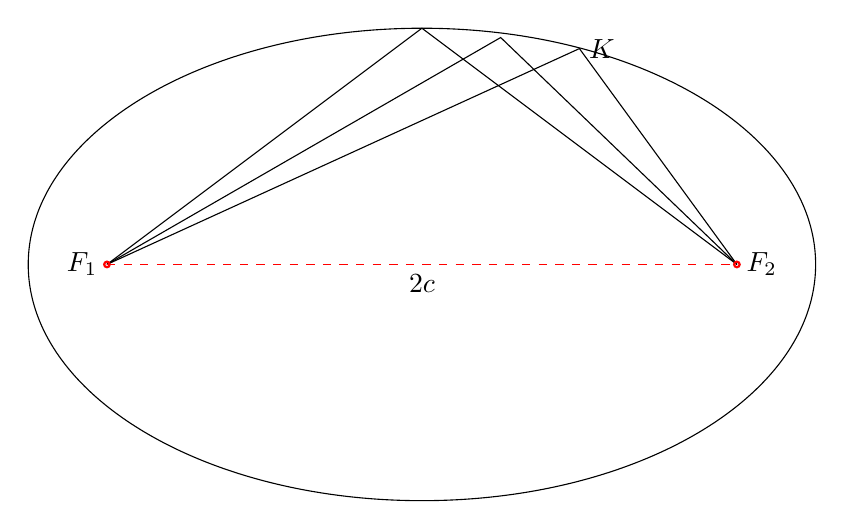
\begin{tikzpicture}

\draw (0,0) ellipse  (5 and 3);

\draw  (-4,0)--(0,3)--(4,0);
\draw  (-4,0)--(1,82pt)--(4,0);
\draw  (-4,0)--(2,78pt)--(4,0);
\node 
[right] 
at (2,78pt) {$K$};

\draw [dashed, red] (-4,0) -- (4,0);
\node [below] at (0,0) {$2c$};

\draw[red,thick] (-4,0) circle (1pt); 
\draw[red,thick] (4,0) circle (1pt); 
\node [left] at (-4,0) {$F_1$};
\node [right] at (4,0) {$F_2$};
\end{tikzpicture}
\end{equation}
   
          $$
       |F_1F_2|=2c\,,\qquad a>c>0\,.
          $$
      

Ellipse $=\{K\colon\quad |KF_1|+|KF_2|=2a\}$

\m

    $F_1$, $F_2$ are foci of ellipse.


      


If $c=0$, ellipse becomes circle.



%\begin{equation}
%\begin{tikzpicture}[scale=1]
%    \pgfmathsetmacro{\e}{1.44022}   % eccentricity
%    \pgfmathsetmacro{\a}{1}
%    \pgfmathsetmacro{\b}{1}%{(\a*sqrt((\e)^2-1)} 
%    \draw [domain=-2:2] plot ({\a*cosh(\x)},{\b*sinh(\x)});    %\draw plot[domain=-2:2] ({-\a*cosh(\x)},{\b*sinh(\x)});
%\end{tikzpicture}
%\end{equation}


 \subsubsection {Hyperbola on the  Euclidean plane}

 Hyperbola on the plane is the locus of all the points
such that the difference of distances from these points to
two fixed points $F_1,F_2$ is equal to given constant.



\begin{equation}\label{firsthyperbola}
\begin{tikzpicture}[scale=0.5]
    \pgfmathsetmacro{\a}{4}
    \pgfmathsetmacro{\b}{3}
    \draw [domain=-2:2] plot ({\a*cosh(\x)},{\b*sinh(\x)});
   \draw plot[domain=-2:2] ({-\a*cosh(\x)},{\b*sinh(\x)});
\draw  (-5,0)--(12,8.46)--(5,0);
\draw  (-5,0)--(-12,8.46)--(5,0);
\draw  (-5,0)--(6,3.3)--(5,0);
\node [right] at (12, 8.46) {$K$};
\draw [dashed, red] (-5,0) -- (5,0);
\node [below] at (0,0) {$2c$};

\draw[red,thick] (-5,0) circle (1pt); 
\draw[red,thick] (5,0) circle (1pt); 
\node [left] at (-5,0) {$F_2$};
\node [right] at (5,0) {$F_1$};
\end{tikzpicture}
\end{equation}


Hyperbola $=\{K\colon\quad \left||KF_1|-|KF_2|\right|=2a\}$

The points $F_1,F_2$ are foci of hyperbola.
 
{\bf Remark} Notice that for ellipse
we denote 
``left'' focus $F_1$ and `'right focus''
$F_2$, and for hyperbola vice versa:
``right'' focus $F_1$ and `'left''  focus
$F_2$. The difference between these two notations
will be important only
when we will consider analytical definitions of
hyperbola, and we will note it later.

 \subsubsection {Parabola  on the  Euclidean plane}

 Parabola on the plane is the locus of all the points
such that they are at the same distance from the given point
   $F$ and the given line $l$.


\begin{equation}\label{firstparabola}
\begin{tikzpicture}%[scale=0.8]
%\draw [help lines] (-5,-5) grid (5,5);
    \draw [domain=-5:5] plot ({0.5*\x*\x-5},\x);
\draw [  thick, blue] (-5.5,-6)--(-5.5,6); 
\node [left] at (-5.5,6) {$l$};
\draw  (-5.5,4)--(3,4)--(-4.5,0);
\draw  (-5.5,-2)--(-3,-2)--(-4.5,0);
\draw  (-5.5,2)--(-3,2)--(-4.5,0);
\node [right] at (-3, 2) {$K$};
\draw[red,thick] (-4.5,0) circle (1pt); 
\node [left] at (-4.5,0) {$F$};
\end{tikzpicture}
\end{equation}

\m


Parabola $=\{K\colon\quad d(K,l)=|KF|\}$

\m       

The point $F$ is called the focus of the parabola,
and the line $l$  is called the {\it directrix of the parabola.}


\m


{\footnotesize  One can consider directrices for hyperbola
and ellipse also. See later subsection\ref{theyarethesame}}

\subsection {Cartesian and affine coordinates in the plane and 
in the space}

\subsubsection {Cartesian coordinates in plane $\E^2$}\label
{cartesiancoordinatesinplane}                      

Consider affine space $\E^2$.

Recall that fixing the point 
in affine space we come to the vector
space $\E^2$(see \ref{affineandvectorspaces}).
 
Let $\{\e_x,\e_y\}$ be an orthonormal basis attached at 
a  point
 $O$. The point $O$ is an origin of this frame of reference.
For every point $A\in \E^2$ we have

\begin{equation}\label{cartesiancoordinatesinplane0}
\begin{tikzpicture}
\draw 
[ <-> , thick] 
(5,0)--(0,0)--(0,5);

\draw [thick, ->,blue] (0,0)--(1,0);
\node [below] at (0.5,0) {$\e_x$};

\draw [thick, ->,blue] (0,0)--(0,1);
\node [left] at (0,0.5) {$\e_y$};

\node [left] at (0,4) {$y$};
\node [below] at (4,0) {$x$};
\node [below] at (0,0) {$O$};

\draw [thick, red,->] (0,0)--(2,3); 
\node [right] at (1,1.5) {$\r$};
\node [right] at (2,3) {$P$};
\end{tikzpicture}\,,\quad
\r=\vec {OA}=x\e_x+y\e_y\,,
\end{equation}
\begin{equation*}
|\e_x|=|\e_y|=1\, {\rm and }\,\,
\angle \left(\e_x,\e_y\right)={\pi\over 2}\,, {\rm i.e.}\,\,
(\e_x,\e_x)=(\e_y,\e_y)=1\,, (\e_x,\e_y)=0\,.
\end{equation*}

Coordinates $x,y$ are Cartesian coordinates of the point
$P$ with respect to frame  $XOY$


\m

 Consider now two frames of references.
Let $\{\e_x,\e_y\}$ be an orthonormal basis attached at 
the point
 $O$, and let
$\{\e'_x,\e'_y\}$ be an orthonormal basis attached at 
the point  $O'$.
 $O$.

\begin{equation*}
\begin{tikzpicture} [rotate=10]
\draw 
[ <-> , thick] 
(5,0)--(0,0)--(0,5);

\draw [thick, ->,blue] (0,0)--(1,0);
\node [below] at (0.5,0) {$\e'_x$};

\draw [thick, ->,blue] (0,0)--(0,1);
\node [left] at (0,0.5) {$\e'_y$};

\node [left] at (0,4) {$y'$};
\node [below] at (4,0) {$x'$};

\node [below] at (0,0) {$O^{\,\,\prime}$};

%\end{tikzpicture}
%\begin{tikzpicture} 
%[rotate=-10]
\draw 
[ <-> , thick] 
(3,8)--(5,3)--(10,5);


\draw [thick, ->,blue] (5,3)--(170pt,96pt);
\node [below] at (160pt,94pt) {$\e_x$};


\draw [thick, ->,blue] (5,3)--(131pt,110pt);
\node [left] at (135pt, 97pt) {$\e_y$};


\node [left] at (4,5.5) {$y$};
\node [below] at (7.5,4) {$x$};
\node [below] at (5,3) {$O$};


\draw [thick, yellow,->] (5,3)--(0,0);



%\draw [help lines] (0,0) grid (12,12);

\end{tikzpicture}
\end{equation*}


Let $A$ be an arbitrary point in the plane
$\E^2$.  We denote:
     $$
\r=\vec {OP}\,,
\r'=\vec {O'P}\,,\quad {\rm and}\,\,
{\bf t}=\vec {OO'}\,.
       $$ 

% a point $A$ in two different Cartesian coordinates
\begin{equation}\label{changingofcartesiancoordinates1}
\begin{tikzpicture} [rotate=10]
\draw 
[ <-> , thick] 
(5,0)--(0,0)--(0,5);

\draw [thick, ->,blue] (0,0)--(1,0);
\node [below] at (0.5,0) {$\e'_x$};

\draw [thick, ->,blue] (0,0)--(0,1);
\node [left] at (0,0.5) {$\e'_y$};

\node [left] at (0,4) {$y'$};
\node [below] at (4,0) {$x'$};

\node [below] at (0,0) {$O^{\,\,\prime}$};

%\end{tikzpicture}
%\begin{tikzpicture} 
%[rotate=-10]
\draw 
[ <-> , thick] 
(3,8)--(5,3)--(10,5);


\draw [thick, ->,blue] (5,3)--(170pt,96pt);
\node [below] at (160pt,94pt) {$\e_x$};


\draw [thick, ->,blue] (5,3)--(131pt,110pt);
\node [left] at (135pt, 97pt) {$\e_y$};


\node [left] at (4,5.5) {$y$};
\node [below] at (7.5,4) {$x$};
\node [below] at (5,3) {$O$};


\draw [thick, yellow,->] (5,3)--(0,0);
\draw [thick, red,->] (0,0)--(6,6);
\draw [thick, red,->] (5,3)--(6,6);

\node [right] at (6,6) {$A$};
\node [below] at (2.5,1.5) {$\bf t$};
\node [below] at (3,3) {$\r'$};
\node [right] at (5.5,4.5) {$\r$};


%\draw [help lines] (0,0) grid (12,12);

\end{tikzpicture}
\end{equation}



We have
  \begin{equation*}
  \r={\bf t}+\r'  
  \end{equation*}
i.e.
 \begin{equation*}
      \underbrace
            {
  (\e_x,\e_y)
  \begin{pmatrix}
         x \cr
        y\cr
   \end{pmatrix}
     }_{\r}
            =
        \underbrace
         {
  (\e_x,\e_y)
      \begin{pmatrix}
         a \cr
        b\cr
   \end{pmatrix}
          }_{\bf t}
          +
      \underbrace
         {
  (\e'_x,\e'_y)
      \begin{pmatrix}
         x' \cr
        y'\cr
   \end{pmatrix}
          }_{\bf \r'}
\end{equation*}\,,
i.e.
  \begin{equation*}
  x\e_x+y\e_y=\r={\bf t}+\r'=a\e_x+b\e_y+x'\e'_x+y'\e'_y\,.
  \end{equation*}
The bases $\{\e_x,\e_y\}$, $\{\e'_x,\e'_y\}$
are related by orthogonal matrix:
      \begin{equation}\label{matrixorthogonal1}
  (\e'_x,\e'_y)=(\e_x,\e_y)
\underbrace
        {
     \begin{pmatrix}
    p_{11} &p_{12}\cr
    p_{21} &p_{22}\cr
\end{pmatrix}
     }_{\hbox {\footnotesize orthog. matr.}}\,.
    \end{equation}

 \begin{equation*}
  (\e_x,\e_y)
  \begin{pmatrix}
         x \cr
        y\cr
   \end{pmatrix}
=  (\e_x,\e_y)
  \begin{pmatrix}
         a \cr
        b\cr
   \end{pmatrix}
              +  
 (\e_x,\e_y)
      \begin{pmatrix}
    p_{11} &p_{12}\cr
    p_{21} &p_{22}\cr
         \end{pmatrix}
           \begin{pmatrix}
         x'\cr
        y'\cr
   \end{pmatrix}\,,
\end{equation*}
i.e. \begin{equation*}
  \begin{pmatrix}
         x \cr
        y\cr
   \end{pmatrix}
         =
  \begin{pmatrix}
         a \cr
        b\cr
   \end{pmatrix}
              +  
         \underbrace
         {
      \begin{pmatrix}
    p_{11} &p_{12}\cr
    p_{21} &p_{22}\cr
         \end{pmatrix}
         }_{\hbox 
    {\footnotesize orthog.matrix}}
           \begin{pmatrix}
         x'\cr
        y'\cr
   \end{pmatrix}\,.
\end{equation*}
 
   \begin{equation*}\label{changingcartesiancoordinatesinplane}
\begin{cases}
    x=a+p_{11}x'+p_{12}y'\cr
    y=b+p_{21}x'+p_{22}y'\cr
 \end{cases}
   \end{equation*}


One can say that changing of coordinates
is translation $+$ rotation (or rotation+ reflection.)


{\bf Example} Consider
in \eqref{matrixorthogonal1}
an orthogonal matrix
       $$
P=     \begin{pmatrix}
    p_{11} &p_{12}\cr
    p_{21} &p_{22}\cr
         \end{pmatrix}=
      \begin{pmatrix}
    \cos\varphi &-\sin\varphi\cr
    \sin\varphi &\cos\varphi\cr
         \end{pmatrix}\,,\quad
       (P^+\circ P={\bf id}\,,\quad {\rm and}
\,\,\det P=1)
         $$ 
($P$ preserves orientation. 
This is rotation on the angle $\varphi$) 

Another example:

{\bf Example}
Consider in
\eqref{changingcartesiancoordinatesinplane},
an orthogonal matrix
       $$
P=     \begin{pmatrix}
    p_{11} &p_{12}\cr
    p_{21} &p_{22}\cr
         \end{pmatrix}=
      \begin{pmatrix}
    \cos\varphi &\sin\varphi\cr
    \sin\varphi &-\cos\varphi\cr
         \end{pmatrix}\,,\quad
       (P^+\circ P={\bf id}\,,\quad {\rm and}
\,\,\det P=-1)
         $$ 
($P$ changes orientation. 
This is rotation and reflection) 




\subsubsection {Cartesian coordinates in $\E^3$}

The analogous considerations  in $\E^3$:

     \begin{equation*}
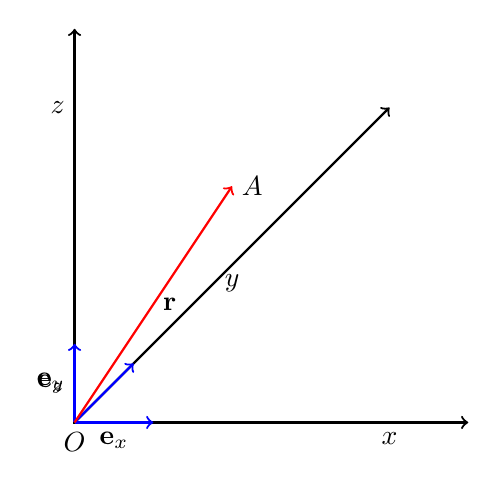
\begin{tikzpicture}
\draw 
[ <-> , thick] 
(5,0)--(0,0)--(0,5);
\draw 
[ -> , thick] 
(0,0)--(4,4);


\draw [thick, ->,blue] (0,0)--(1,0);
\node [below] at (0.5,0) {$\e_x$};

\draw [thick, ->,blue] (0,0)--(0,1);
\node [left] at (0,0.5) {$\e_z$};

\draw [thick, ->,blue] (0,0)--(0.75,0.75);
\node [left] at (0,0.5) {$\e_y$};

\node [left] at (0,4) {$z$};
\node [below] at (4,0) {$x$};
\node [below] at (2,2) {$y$};
\node [below] at (0,0) {$O$};

\draw [thick, red,->] (0,0)--(2,3); 
\node [right] at (1,1.5) {$\r$};
\node [right] at (2,3) {$A$};
\end{tikzpicture}\,,
\r=\vec {OA}=x\e_x+y\e_y+z\e_z\,,
\end{equation*}
\begin{equation*}
|\e_x|=|\e_y|=|\e_z|=1\, {\rm and }\,\,
\angle \left(\e_x,\e_y\right)=
\angle \left(\e_x,\e_z\right)=
\angle \left(\e_y,\e_z\right))={\pi\over 2}\,,
    \end{equation*} 
i.e.
   \begin{equation*}
(\e_x,\e_x)=(\e_y,\e_y)=1\,, (\e_z,\e_z)=1\,,
(\e_x,\e_y)=(\e_x,\e_z)=(\e_y,\e_z)=0\,.
\end{equation*}
  We have that $\{\e_x,\e_y,\e_z\}$ is an orthonormal basis
and $x,y,z$ are Cartesian coordinates of point
$A$ with respect to frame  $OXYZ$.


\m




  Now coonsider two different Cartesian coordinates
 


Let in $\E^3$, ${\e_x,\e_y,\e_z}$ be an orthonormal 
frame with  the origin at the point $O$
and let ${\e'_x,\e'_y.\e'_z}$ be an another
orthonormal 
frame with the origin at the the point $O'$:

%two different coordinates
\begin{equation*}
%%%the second frame
\begin{tikzpicture} [rotate=10]
\draw 
[ <-> , thick] 
(8,0)--(0,0)--(0,8);
\draw 
[ -> , thick] 
(0,0)--(5,5);


\draw [thick, ->,blue] (0,0)--(1,0);
\node [below] at (1,0) {$\e'_x$};

\draw [thick, ->,blue] (0,0)--(0,1);
\node [left] at (0,1) {$\e'_z$};

\draw [thick, ->,blue] (0,0)--(0.8,0.8);
\node [left] at (0.4,0.4) {$\e'_y$};


\node [below] at (7,0) {$x'$};
\node [left] at (0,7) {$z'$};
\node [left] at (4,4) {$y'$};


\node [below] at (0,0) {$O^{\,\,\prime}$};


% the first frame
 
\draw 
[ <-> , thick] 
(13,-1)--(5,1)--(7,9);
\draw 
[ -> , thick] 
(5,1)--(10,4);


\draw [thick, ->,blue] (5,1)--(6,21pt);
\node [below] at (6,21pt) {$\e_x$};

\draw [thick, ->,blue] (5,1)--(150pt,2);
\node [left] at (150pt,2) {$\e_z$};

\draw [thick, ->,blue] (5,1)--(6,46pt);
\node [left] at (6,46pt) {$\e_y$};


\node [below] at (13,-1) {$x$};
\node [left] at (7,9) {$z$};
\node [left] at (10,4) {$y$};


\node [below] at (5,1) {$O$};

\draw [thick, yellow,->] (5,1)--(0,0);


\node [below] at (2.5,0.5) {$\bf t$};


%\draw [help lines] (-2,-2) grid (12,12);
\end{tikzpicture}
\end{equation*}

  Let $A$ be an arbitrary point in $\E^3$.

  Denote by
       $$
\r=\vec {OA}\,,
\r'=\vec {O'A}\,,\quad {\rm and}\,\,
{\bf t}=\vec {OO'}\,.
       $$ 

%a point in two different coordinates
\begin{equation*}
%%%the second frame
\begin{tikzpicture} [rotate=10]
\draw 
[ <-> , thick] 
(8,0)--(0,0)--(0,8);
\draw 
[ -> , thick] 
(0,0)--(5,5);


\draw [thick, ->,blue] (0,0)--(1,0);
\node [below] at (1,0) {$\e'_x$};

\draw [thick, ->,blue] (0,0)--(0,1);
\node [left] at (0,1) {$\e'_z$};

\draw [thick, ->,blue] (0,0)--(0.8,0.8);
\node [left] at (0.4,0.4) {$\e'_y$};


\node [below] at (7,0) {$x'$};
\node [left] at (0,7) {$z'$};
\node [left] at (4,4) {$y'$};


\node [below] at (0,0) {$O^{\,\,\prime}$};


% the first frame
 
\draw 
[ <-> , thick] 
(13,-1)--(5,1)--(7,9);
\draw 
[ -> , thick] 
(5,1)--(10,4);


\draw [thick, ->,blue] (5,1)--(6,21pt);
\node [below] at (6,21pt) {$\e_x$};

\draw [thick, ->,blue] (5,1)--(150pt,2);
\node [left] at (150pt,2) {$\e_z$};

\draw [thick, ->,blue] (5,1)--(6,46pt);
\node [left] at (6,46pt) {$\e_y$};


\node [below] at (13,-1) {$x$};
\node [left] at (7,9) {$z$};
\node [left] at (10,4) {$y$};


\node [below] at (5,1) {$O$};

\draw [thick, yellow,->] (5,1)--(0,0);
\draw [thick, red,->] (0,0)--(7,4);
\draw [thick, red,->] (5,1)--(7,4);


\node [below] at (2.5,0.5) {$\bf t$};
\node [below] at (3.5,2) {$ \r'$};
\node [below] at (3.5,2) {$\r$};
\node [below] at (7,4) {$A$};


%\draw [help lines] (-2,-2) grid (12,12);
\end{tikzpicture}
\end{equation*}

We have in the same way as in $\E^2$:

  \begin{equation*}
  \r={\bf t}+\r'  
  \end{equation*}
i.e.
 \begin{equation*}
      \underbrace
            {
  (\e_x,\e_y,\e_z)
  \begin{pmatrix}
         x \cr
        y\cr
        z\cr
   \end{pmatrix}
     }_{\r}
            =
        \underbrace
         {
  (\e_x,\e_y,\e_z)
      \begin{pmatrix}
         a \cr
        b\cr
         c\cr
   \end{pmatrix}
          }_{\bf  t}
          +
      \underbrace
         {
  (\e'_x,\e'_y,\e'_z)
      \begin{pmatrix}
         x' \cr
        y'\cr
        z'
   \end{pmatrix}
          }_{\bf \r'}
\end{equation*}\,,
i.e.
  \begin{equation*}
  x\e_x+y\e_y+z\e_z=\r=
{\bf t}+\r'=a\e_x+b\e_y+c\e_z=
     x'\e'_x+y'\e'_y+z'\e'_z\,.
  \end{equation*}
The orthonormal 
bases $\{\e_x,\e_y,\e_z\}$, $\{\e'_x,\e'_y,\e_z\}$
are related by orthogonal matrix:
      \begin{equation*}
  (\e'_x,\e'_y,\e'_z)=(\e_x,\e_y,\e_z)
\underbrace
        {
     \begin{pmatrix}
    p_{11} &p_{12} &p_{13}\cr
    p_{21} &p_{22} &p_{23}\cr
    p_{31} &p_{32} &p_{33}\cr
\end{pmatrix}
     }_{\hbox {\footnotesize orthog. matr.}}\,.
    \end{equation*}
Thus
 \begin{equation*}
  (\e_x,\e_y,\e_z)
  \begin{pmatrix}
         x \cr
        y\cr
            z\cr
   \end{pmatrix}
=  (\e_x,\e_y,\e_z)
  \begin{pmatrix}
         a \cr
        b\cr
        c\cr
   \end{pmatrix}
              +  
 (\e_x,\e_y,\e_z)
      \begin{pmatrix}
    p_{11} &p_{12} &p_{13}\cr
    p_{21} &p_{22} &p_{23}\cr
    p_{31} &p_{32} &p_{33}\cr
         \end{pmatrix}
           \begin{pmatrix}
         x'\cr
        y'\cr
           z'\cr
   \end{pmatrix}\,,
\end{equation*}
i.e. \begin{equation*}
  \begin{pmatrix}
         x \cr
        y\cr
       z\cr
   \end{pmatrix}
         =
  \begin{pmatrix}
         a \cr
        b\cr
       c\cr
   \end{pmatrix}
              +  
         \underbrace
         {
      \begin{pmatrix}
    p_{11} &p_{12} &p_{13}\cr
    p_{21} &p_{22} &p_{23}\cr
    p_{31} &p_{32} &p_{33}\cr
         \end{pmatrix}
         }_{\hbox 
    {\footnotesize orthog.matrix}}
           \begin{pmatrix}
         x'\cr
         y'\cr
         z'\cr
   \end{pmatrix}\,,
\end{equation*}
\begin{equation}\label{changingcartesiancoordinatesinspace}
\begin{cases}
    x=a+p_{11}x'+p_{12}y'+p_{13}z'\cr
    y=b+p_{21}x'+p_{22}y'+p_{23}z'\cr
    z=c+p_{31}x'+p_{32}y'+p_{33}z'\cr
 \end{cases}
   \end{equation}




Recalling Euler Theorem one 
One can say that changing  of coordinates
is translation $+$ rotation (or rotation+ reflection.)



\m

  Consider examples of transformation
\eqref{changingcartesiancoordinatesinspace}


Rotation arond axis $Oz$ on the angle $\varphi$:
\begin{equation*}
  \begin{pmatrix}
         x \cr
        y\cr
       z\cr
   \end{pmatrix}
         =
      \begin{pmatrix}
    \cos\varphi &-\sin\varphi &0\cr
    \sin\varphi &\cos\varphi &0\cr
    0 &0 &1\cr
         \end{pmatrix}
           \begin{pmatrix}
         x'\cr
        y'\cr
        z'\cr
   \end{pmatrix}\,.
\end{equation*}

Another example:

Rotation arond axis $Oz$ on the angle $\pi\over 6$
and translation:
\begin{equation*}
  \begin{pmatrix}
         x \cr
        y\cr
       z\cr
   \end{pmatrix}
         =
  \begin{pmatrix}
         a \cr
        b\cr
       c\cr
   \end{pmatrix}
              +  
      \begin{pmatrix}
    1 &0 & 0\cr
    0 &{\sqrt 3\over 2} &-{1\over 2}\cr
    0 &{1\over 2} &{\sqrt 3\over 2}\cr
         \end{pmatrix}
           \begin{pmatrix}
         x'\cr
        y'\cr
        z'\cr
   \end{pmatrix}\,,
\end{equation*}

\subsubsection{Arbitrary affine coordinates}
 We consider in
\eqref{changingcartesiancoordinatesinplane}
\eqref{changingcartesiancoordinatesinspace}
changing of Cartesian coorindates from one orthonormal
basis to another. In the general case if bases are not orthonormal
we have coordinates hich are not Cartesian, they are just
so called {\it affine} coordinates.
  We consider affine coordinates in the plane $\E^2$.

   Affine coordinates of the point:
\begin{equation*}
\begin{tikzpicture}
\draw 
[ <-> , thick] 
(10,0)--(0,0)--(6,8);

\draw [thick, ->,blue] (0,0)--(2,0);
\node [below] at (0.5,0) {$\e_x$};

\draw [thick, ->,blue] (0,0)--(0.75,1);
\node [left] at (0,0.5) {$\e_y$};

\node [left] at (5,7) {$y$};
\node [below] at (4,0) {$x$};
\node [below] at (0,0) {$O$};

\draw [thick, red,->] (0,0)--(5,2); 
\node [right] at (1,1.5) {$\r$};
\node [right] at (5,2) {$A$};
\end{tikzpicture}\,,\quad
\r=\vec {OA}=x\e_x+y\e_y\,,
\end{equation*}
In this case 
$\{\e_x,\e_y\}$ is not in general an orthonormal basis:
the vectors $\e_x,\e_y$ may have an 
arbitrary length, and the angle $\theta$ 
between them may be an abritrary. 
Sure the vectors $\e_x,\e_y$ 
have to be linearly independent, since
$\{\e_x,\e_y\}$ is a basis, this is why
  $|\e_x|\not=0$, 
$|\e_y|\not=0$ and $\theta\not=0$. 
In the special case if 
these vectors are unit vectors and angle between them
is equal to $\pi\over 2$ we come to Cartesian coordinates
\eqref{cartesiancoordinatesinplane0}

\m


Write down the formulae of changing coordinates
if we change the coordinate systems.

Let $OXY$ be coordinate frame with the origin at the point
$O$ and with basic vectors $\{\e_x,\e_y\}$,
and let $O'X'Y'$ be coordinate frame with origin at the point
$O'$ and with basic vectors $\{\e'_x,\e'_y\}$,
(Compare with \eqref{changingofcartesiancoordinates1}).

In the same way as in \eqref{changingofcartesiancoordinates1} 
we have  \begin{equation*}
  \r={\bf t}+\r'  
  \end{equation*}
i.e.
 \begin{equation*}
      \underbrace
            {
  (\e_x,\e_y)
  \begin{pmatrix}
         x \cr
        y\cr
   \end{pmatrix}
     }_{\r}
            =
        \underbrace
         {
  (\e_x,\e_y)
      \begin{pmatrix}
         a \cr
        b\cr
   \end{pmatrix}
          }_{\bf t}
          +
      \underbrace
         {
  (\e'_x,\e'_y)
      \begin{pmatrix}
         x' \cr
        y'\cr
   \end{pmatrix}
          }_{\bf \r'}
\end{equation*}\,,
i.e.
  \begin{equation*}
  x\e_x+y\e_y=\r={\bf t}+\r'=a\e_x+b\e_y+x'\e'_x+y'\e'_y\,.
  \end{equation*}
In this case the bases $\{\e_x,\e_y\}$, $\{\e'_x,\e'_y\}$
are related by non-degenerate  matrix:
      \begin{equation}\label{matrixnondegenerate1}
  (\e'_x,\e'_y)=(\e_x,\e_y)
\underbrace
        {
     \begin{pmatrix}
    p_{11} &p_{12}\cr
    p_{21} &p_{22}\cr
\end{pmatrix}
     }_{\det P\not=0}\,,
    \end{equation}
and
 \begin{equation*}
  (\e_x,\e_y)
  \begin{pmatrix}
         x \cr
        y\cr
   \end{pmatrix}
=  (\e_x,\e_y)
  \begin{pmatrix}
         a \cr
        b\cr
   \end{pmatrix}
              +  
 (\e_x,\e_y)
      \begin{pmatrix}
    p_{11} &p_{12}\cr
    p_{21} &p_{22}\cr
         \end{pmatrix}
           \begin{pmatrix}
         x'\cr
        y'\cr
   \end{pmatrix}\,,
\end{equation*}
i.e. \begin{equation*}
  \begin{pmatrix}
         x \cr
        y\cr
   \end{pmatrix}
         =
  \begin{pmatrix}
         a \cr
        b\cr
   \end{pmatrix}
              +  
         \underbrace
         {
      \begin{pmatrix}
    p_{11} &p_{12}\cr
    p_{21} &p_{22}\cr
         \end{pmatrix}
         }_{\hbox 
    {\footnotesize non-degenerate matrix}}
           \begin{pmatrix}
         x'\cr
        y'\cr
   \end{pmatrix}\,.
\end{equation*}
 
   \begin{equation}\label{changingcartesiancoordinatesinplane}
\begin{cases}
    x=a+p_{11}x'+p_{12}y'\cr
    y=b+p_{21}x'+p_{22}y'\cr
 \end{cases}
   \end{equation}

 The difference with the case of 
changing of Cartesian coordinates
considered in subsection \ref{cartesiancoordinatesinplane}
(see \eqref{matrixorthogonal1}) 
is the following: in the case of changing of Cartesian
 coordinates, the matrix $P$ in equation 
\eqref{matrixorthogonal1} is orthogonal matrix,
since it is transition matrix between two orthonormal
bases, 
and the matrix $P$ in equation \eqref{matrixnondegenerate1}
is just non-degenerate transition matrix between two bases.          

\subsubsection {Affine coordiantes and area of ellipse}\label{area1}

  We consider in this subsection one very important example.

Consider an ellipse 
       \begin{equation}\label{thisellipse}
{x^2\over a^2}+{y^2\over b^2}=1\,.
         \end{equation}
in Cartesian coordinates.
(We will consider this equation
of ellipse later in detail. Now we just 
use very simple
properties of this formula to come to the formula
for area of ellipse (more precisely the area of
the domain restircted by
this ellipse).)
Under  affine transformations
   \begin{equation}\label{ellipsetocircle}
\begin{cases}x=au\cr y=bv\cr\end{cases}
   \end{equation}\,,\quad (a,b>0)
the ellipse becomes the circle $u^2+v^2=1$, and
the area of the interior of the unit circle
circle is equal to $\pi$.
             $$
\hbox {Area of the interior of the 
ellipse \eqref{thisellipse}}=
 \int_{
{x^2\over a^2}+{y^2\over b^2}\leq 1}dxdy=
 \int_{u^2+v^2\leq 1} 
\left|{\p (x,u)\over \p (u,v)}\right|dudv=
             $$
    \begin{equation*}
 \int_{u^2+v^2\leq 1} 
\left|\det \begin{pmatrix} 
 {\p x\over \p u}&{\p x\over \p v}\cr
 {\p y\over \p u}& {\p y\over \p v}\cr
      \end{pmatrix}    \right|dudv=
 \int_{u^2+v^2\leq 1} 
\left|\det \begin{pmatrix} 
 a&0\cr
 0& b\cr
      \end{pmatrix}    \right|dudv=
      \end{equation*}
       \begin{equation}\label{areaofellipse}
ab  \int_{u^2+v^2\leq 1} 
         dudv=
ab\cdot \hbox{ \{Area of the interior of the 
unit circle\}}=\pi ab\,.   
      \end{equation}
Indeed one can see it without using integration formulae:
the affine transformation \eqref{ellipsetocircle}
changes size in $OX$ direction $a$ times and it changes the
size in  $OY$ direction in $b$ times, hence area of changing 
 $ab$ times, i.e. area of the ellipse is equal to $\pi ab$.




\subsection{Analytical definition of conic sections}
\label{analyticdefinitions}

%\end{document} %26 March 2018
We will define here conic sections analytically and will proof
that the equivalence of analytical and geometrical definitions.

    We will call ellipse, hyperbola and parabola
  {\tt conic sections.}
This terminology will be explained in the next lecture.

  We have given above geometric definitions of 
  conic sections  (see \eqref{firstellipse}, \eqref{firsthyperbola} 
and \eqref{firstparabola}). Now we give
anaytical definitions of conic sections.

\m

\centerline {\it Definitions}

\m

{\bf Definition}  
Let $C$ be a curve on the plane. 
The  curve $C$ is an ellipse if {\it there exist
Cartesian coordinates $(x,y)$ on the plane},
such that in these Cartesian coordinates
this curve is defined by canonical  equation
     \begin{equation}\label{analytell}
   {x^2\over a^2}+{y^2\over b^2}=1\,,
     \end{equation}
where $a,b$ are positive numbers such that  $a\geq b$.

\m

{\bf Definition}  
Let $C$ be a curve on the plane. 
The  curve $C$ is a hyperbola  {\it if there exist
Cartesian coordinates $(x,y)$ on the plane},
such that in these Cartesian coordinates
this curve is defined by canonical equation
     \begin{equation}\label{analythyp}
   {x^2\over a^2}-{y^2\over b^2}=1\,,
     \end{equation}
where $a,b$ are positive numbers.


\m


\m

{\bf Definition}  
Let $C$ be a curve on the plane. 
The  curve $C$ is a parabola  {\it if there exist
Cartesian coordinates $(x,y)$ on the plane},
such that in these Cartesian coordinates
this curve is defined by canonical equation
     \begin{equation}\label{analytparabola}
   y^2=2px\,,  p>0\,.
     \end{equation}
where $p$ is a  positive number
\footnote{We usually in school, considered parabola as
$y=ax^2$. Traditionally in anaylical geometry parabola is
cosnidered with twistex axis $x\leftrightarrow y$.}.

$$ $$

{\bf Proposition}

{\it Geometrical and analytical definitions of conic
sections are equivalent.
}

We will prove this Proposition separately for ellipse, hyperbola
and parabola.

\subsubsection {Equivalence of analytical and 
geometrical definitions for ellipse}\label{equivofdefforellipse}



Let $C$ be an ellipse defined geometrically:
         \begin{equation}\label{geomellipse2}
C=\{K\colon\quad |KF_1|+|KF_2|=2a\}
           \end{equation}

Consider Cartesian coordinates, such that
origin is at the middle of the segment $F_1F_2$,
axis $OX$ is along foci from $F_1$ to $F_2$:
$x$ coordinates of  the point $F_1$ is negative and 
$x$ coordinate of the point $F_2$ is positive.
   \begin{equation*}
    \begin{tikzpicture}
%\draw [help lines] (-4,-4) grid (8,6);

   \draw       [->] (-6,0)--(0,0)--(6,0); 
   \draw       [->] (0,-4)--(0,0)--(0,4); 
 \node [below] at (5,0)   {$x$};    
 \node  [right] at (0,3) {$y$};    
\draw (-2,0) circle (1pt);
\node [below] at (-2,0) {$F_1$}; 
\draw (2,0) circle (1pt);
\node [below] at (2,0) {$F_2$}; 

\draw (0,0) ellipse  (2.5 and 1.5);

\draw [red] (-2,0)--(1,1.3)--(2,0);
\node [right] at (1,1.3) {$K$};
\end{tikzpicture} 
     \end{equation*} 
      $$
F_1=(-c,0)\,, F_2=(c,0)\,,  K=(x,y)\,.
      $$
We may suppose that
    \begin{equation}\label{ellipseinequality}
        a>c\,.
    \end{equation}
     Indeed it follows from the triangle $F_1KF_2$ that
$2a=|KF_1|+|KF_2|\geq |F_1F_2|=2c$.
(In the case if $a=c$ ellipse degenerates to the segment
$(F_1F_2)$.

  We have 
     $$
|KF_1|+|KF_2|=
\sqrt{(x+c)^2+y^2}+
\sqrt{(x-c)^2+y^2}=2a\,, (a\geq c>0)\,.
      $$
Hence
\begin{equation}\label{calcforellipse1}
\sqrt{(x+c)^2+y^2}=2a-
\sqrt{(x-c)^2+y^2}\,.
       \end{equation}  
     Take square:
           $$
  x^2+2xc+c^2=4a^2+x^2-2xc+c^2+y^2-4a\sqrt{(x-c)^2+y^2}\,.
        $$
Hence
          $$
  4a\sqrt{(x-c)^2+y^2}=4a^2-4xc=4(a^2-xc)\,.
        $$
Take again square:
          $$
        a^2\left(x^2-2xc+c^2+y^2\right)=
       a^4-2a^2xc+x^2c^2\,.
         $$
Hence
     \begin{equation}\label{calcforellipse2}
 (a^2-c^2)x^2+a^2y^2=a^4-a^2c^2=a^2(a^2-c^2)\,.
     \end{equation}
Bearing in mind that $a>c$ (see \eqref{ellipseinequality})
we come to 
       \begin{equation}\label{ellipseanal2}
     {x^2\over a^2}+{x^2\over b^2}=1\,, {\rm where}\quad
    b^2=a^2-c^2\,.
     \end{equation}
Thus we proved that all points belonging to the 
locus \eqref{geomellipse2} obey equation
\eqref{analytell}.





One can see that converse implication is also true.
Indeed suppose that for the point $K=(x,y)$
equation \eqref{analytell} is obeyed.
  Then $$
   y^2=b^2\left(1-{x^2\over a^2}\right)\,.
       $$
We have:
             $$
|KF_1|=\sqrt{(x+c)^2+y^2}=
\sqrt{(x+c)^2+b^2\left(1-{x^2\over a^2}\right)}=
        $$
        $$
\sqrt{
  \underbrace{\left(1-{b^2\over a^2}\right)}_{c^2/a^2}
   x^2+2cx+
    \underbrace{c^2+b^2}_{a^2}
       }=
\sqrt{{c^2\over a^2}x^2+2cx+a^2}=
           $$
            \begin{equation}\label{calcforellipse3}
   \sqrt{\left({c\over a}x+a\right)^2}
     =\left|{c\over a}x+a\right|={c\over a}x+a
      \end{equation}
 since $-a<x<a$.

Analogously:             $$
|KF_2|=\sqrt{(x-c)^2+y^2}=
\sqrt{(x-c)^2+b^2\left(1-{x^2\over a^2}\right)}=
        $$
        $$
\sqrt{
 {\left(1-{b^2\over a^2}\right)}+
   x^2-2cx+
  {c^2+b^2}}=
\sqrt{{c^2\over a^2}x^2-2cx+a^2}=
           $$
             \begin{equation}\label{calcforellipse4}
   \sqrt{\left({c\over a}x-a\right)^2}
     =\left|{c\over a}x-a\right|=a-{c\over a}x
       \end{equation}
 since $-a<x<a$.

Hence
       $$
     |KF_1|+|KF_2|=
     \left({c\over a}x+a\right)+
     \left(a-{c\over a}x\right)=2a\,.
       $$
Thus we establish the euqivalence of 
analytical and geometrical definiiton of ellipse.

Two words about the formula for area for ellipse
 which we obtained in ....


 If ellipse is given by analytical formula,
then $a$ is the length of its semi-major axis,
$b$ is the length of its semi-minor axis. 

\subsubsection {$^*$ Equivalence of analytical and 
geometrical definitions for hyperbola}

{\footnotesize  Let $C$ be a hyperbola  defined geometrically:
         \begin{equation}\label{geomhyp2}
C=\{K\colon\quad \left|\,\left|KF_1\right|-
\left|KF_2\right|\,\right|=2a\}
           \end{equation}
Consider Cartesian coordinates, such that
origin is at the middle of the segment $F_1F_2$,
axis $OX$ is along foci in the direction from $F_2$
to $F_1$:
      $$
F_1=(c,0)\,, F_2=(-c,0)\,,  K=(x,y)\,.
      $$
{\bf Remark} Notice that for hyperbola we 
consider $F_1$
with positive coordinate, and $F_2$ with negative
  $x$ coordinate, i.e. 
 we suppose that $F_1$ is ``right'' focus and
$F_2$  is ``left'' focus, and for ellipse it
was vice versa (see \eqref{firstellipse} and 
\eqref{firsthyperbola}). This difference will be imprortant
only when we will consider polar coordinates for hyperbola.


 

We may suppose that
    \begin{equation}\label{hyperbolainequality}
        c>a\,.
    \end{equation}
     Indeed it follows from the triangle $F_1KF_2$ that
$2a=\left||KF_1|-|KF_2||\leq  |F_1F_2|\right|=2c$.
In the case if $a=c$ hyperbola  degenerates to 
two semi-intervals
$C=(-\infty, F_1)\cup (F_2, \infty)$.

We have that 
        $$
\left||KF_1|-|KF_2|\right|=
\sqrt{(x+c)^2+y^2}-
\sqrt{(x-c)^2+y^2}=2a\,.
      $$
Hence
      $$
\sqrt{(x+c)^2+y^2}=2a-
\sqrt{(x-c)^2+y^2}\,.
         $$
This is just equation \eqref{calcforellipse1}:
the difference is that for ellipse we had condition
  $a>c$ (see \eqref{ellipseinequality}); 
now it is condition $c>a$.
Hence we come to the equation \eqref{calcforellipse2}
              $$
\sqrt{(x+c)^2+y^2}=2a-
\sqrt{(x-c)^2+y^2}\Rightarrow
  (c^2-a^2)x^2-a^2y^2=a^2(c^2-a^2)\,,
           $$  
Here just $c>a$.
Dividing on $a^2(c^2-a^2)$ we come to 
    \begin{equation}\label{ellipseanal2}
     {x^2\over a^2}-{y^2\over b^2}=1\,, {\rm where}\quad
    b^2=c^2-a^2\,.
     \end{equation}
Thus we proved that all points belonging to the 
locus \eqref{geomhyp2} obey equation
\eqref{analythyp}.

Now prove converse implication, i.e. that
the points $K=(x,y)$ which   obey equation
 \eqref{analythyp} obey also equation \eqref{geomhyp2}.

The calculations are same that for ellipse 
(see formulae \eqref{calcforellipse3},
\eqref{calcforellipse4})
just that for hyperbola $c>a$, and 
$b^2=c^2-a^2$\footnote{it is useful sometimes to consider hyperbola
as ellipse with $b\mapsto \sqrt {-1}b$}:
             $$
|KF_{1,2}|=\sqrt{(x\pm c)^2+y^2}=
\sqrt{(x\pm c)^2+b^2\left({x^2\over a^2}-1\right)}=
        $$
        $$
\sqrt{
  \underbrace{\left(1+{b^2\over a^2}\right)}_{c^2/a^2}
   x^2\pm 2cx+
    \underbrace{c^2-b^2}_{a^2}
       }=
\sqrt{{c^2\over a^2}x^2\pm 2cx+a^2}=
           $$
            \begin{equation*}\label{calcforhyp3}
   \sqrt{\left(\pm {c\over a}x+a\right)^2}
     =\left|\pm{c\over a}x+a\right|\,.
      \end{equation*}
This implies that
       $$
     ||KF_1|-|KF_2||
         =2a\,.
       $$
}


\subsubsection { Equivalence of analytical and 
geometrical definitions for parabola}

Let $C$ be a parabola   defined geometrically:
         \begin{equation*}\label{geomparabola}
C=\{K\colon\quad d(K,l)=d(K,F)\}\,,
           \end{equation*}
where $l$ is directrix, and $F$ is focus of the parabola.



Let
$T$ be a point on the directrix $l$ such that
the line $FT$ is orthogonal to the directrix $l$.


Consider Cartesian coordinates, such that
the origin is at the middle of the segment $TF$,
and axis  $OX$ goes  along the line $TF$ in the direction
from the point $T$ to the point  $F$:
\begin{equation*}\label{secondparabola}
\begin{tikzpicture}%[scale=0.8]
%\draw [help lines] (-5,-5) grid (5,5);
    \draw [domain=-5:5] plot ({0.25*\x*\x-3},\x);
\draw [ thick, blue] (-4,-6)--(-4,6); 
\node [left] at (-4,5) {$l$};
\draw  (-2,0)--(0,3.48)--(-4,3.48);
%\draw  (-5.5,-2)--(-3,-2)--(-4.5,0);
%\draw  (-5.5,2)--(-3,2)--(-4.5,0);
\node [right] at (0,3.48) {$K$};
\draw[red,thick] (-2,0) circle (1pt); 
\node [left] at (-2,0) {$F$};
\draw[yellow,thick] (-4,0) circle (1pt); 
\node [left] at (-4,0) {$T$};
   \draw       [->] (-6,0)--(0,0)--(6,0); 
   \draw       [->] (-3,-6)--(-3,0)--(-3,6); 
 \node [below] at (5,0)   {$x$};    
 \node  [right] at (-3,5) {$y$};    
\end{tikzpicture}
\end{equation*}
      $$
F=\left({p\over 2},0\right)\,, 
T=\left(-{p\over 2},0\right)\,, 
l\colon x=-{p\over 2}\,, K=(x,y)\,.
      $$
The distancce $d(K,F)=\sqrt {y^2+\left(x-{p\over 2}\right)^2}$.
Note that if  $x<0$, then evidently  $d(K,l)<|KF|$,
hence for the points of the locus of the parabola, $y>0$.
and the distance between point $K$ and directrix 
is equal to $x+p$:  We have
      $$
d(K,F)=\sqrt {y^2+\left(x-{p\over 2}\right)^2}=
d(K,l)=
x+{p\over 2}\Rightarrow  y^2-2px=0\,.
      $$
The converse implication is evident also: If 
for the point $K=(x,y)$, $y^2-2px=0$ ($p>0$), then
         $$
d(K,F)=
\sqrt{y^2+\left(x-{p\over 2}\right)^2}=
\sqrt{2px+\left(x-{p\over 2}\right)^2}=
\sqrt{\left(x+{p\over 2}\right)^2}=
\left|x+{p\over 2}\right|=d(K,l)\,.
         $$
\subsubsection {Resum\'e}\label{resume}

We see that conic sections can be described geometrically
and analytically in suitable canonical Cartesian coordinates:
        \begin{equation}\label{canonicalparameters}
        \begin{matrix}
 &    \hbox{{\tt Geom. definition}}  
&     \hbox{{\tt Analyt.  definition}}  
&     \hbox{{\tt Parameters}} & \cr
\hbox { Ellipse} 
&\{K\colon |KF_1|+|KF_2|=2a\} 
& {x^2\over a^2}+{y^2\over b^2}=1\,
&  |F_1F_2|=2c\,, b^2=a^2-c^2\cr 
\phantom {dfffff}\cr
\hbox { Hyperbola} 
&\{K\colon |\,|KF_1|-|KF_2|\,|=2a\} 
& {x^2\over a^2}-{y^2\over b^2}=1\,
&  |F_1F_2|=2c\,, b^2=c^2-a^2\cr 
\phantom {dfffff}\cr
\hbox { Parabola} 
&\{K\colon |KF|=d(K,l)\} 
& y^2=2px\,
&  d(F,l)=p\cr  
         \end{matrix}
  \end{equation}

We will call these parameters {\it canonical} parameters
of conic sections.

\subsubsection {Area of ellipse, again}

We obtained in paragraph\ref{area1} formula 
\eqref{areaofellipse}
for area of ellipse assuming that for an arbitrry ellipse there 
exist Cartesian coordinates $(x,y)$
such that in these coordinates, the ellipse is defined
by canonical formula ${x^2\over a^2}+{y^2\over b^2}=1$ 
(see equation \eqref{analytell}).
 We proved this statement little bit later in
paragraph \ref{equivofdefforellipse}.
  It is useful again recall this formula
on the base of these conisderations and to fix
notations.  Let
$C$ be an ellipse:

\begin{equation}\label{axesofellipse}
\begin{tikzpicture}

\draw (0,0) ellipse  (5 and 4);
%\draw [help lines] (-4,-4) grid (8,6);
\draw  (-3,0)--(2,3.7)--(3,0);
%\draw  (-4,0)--(1,82pt)--(4,0);
%\draw  (-4,0)--(2,78pt)--(4,0);
\node 
[right] 
at (2,3.7) {$K$};

\draw [dashed, red] (-3,0) -- (3,0);
%\node [below] at (0,0) {$2c$};

\draw[red,thick] (-3,0) circle (1pt); 
\draw[red,thick] (3,0) circle (1pt); 
\node [left] at (-3,0) {$F_1$};
\node [right] at (3,0) {$F_2$};

% coordinates
%\draw [->] (0,-4)--(0,5);
%\node [left] at  (0,3) {$y$};
%\draw [->] (-6,0)--(6,0);
%\node [below] at (4,0) {$x$};

% points of ellipse
\draw[thick] (0,0) circle (1pt); 
\node [below] at  (-0.1,0) {$O$}; % centre

\draw[thick,green] (5,0) circle (1pt); 
\node [below] at  (5.1,0) {$A$}; % rightvertex

\draw[thick,green] (-5,0) circle (1pt); 
\node [below] at  (-5.15,0) {$A'$}; % left vertex

\draw[thick,green] (0,4) circle (1pt); 
\node [above] at  (0,4) {$B$}; % above co-vertex

\draw[thick,green] (0,-4) circle (1pt); 
\node [below] at  (0,-4) {$B'$}; % below co-vertex



\end{tikzpicture}
\end{equation}
   
          $$
\hbox{foci} \qquad F_1,F_2,\,\,|F_1F_2|=2c\,,
  \quad
 \forall K\in C\,\,,  |F_1K|+|KF_2|=2a\,
        a>c>0\,.  
        $$
        $$
\hbox {centre of the ellipse}---O\,,\quad
      |F_1O|=|OF_2|=c\,,
          $$
             $$
\hbox{major axis} \quad |A'A|=2a\,,\qquad
\hbox {semi-major axis}\quad  |OA|=a\,, 
          $$     
          $$
\hbox{minor  axis} \quad |B'B|=2b\,,\qquad
\hbox {semi-minor axis}\quad  |OB|=a\,, 
          $$    
One can consider Cartesian coordinates
$(x,y)$ such that in these coordinates
 the ellipse $C$ is defined by canonical equation

\begin{tikzpicture}

\draw (0,0) ellipse  (5 and 4);
%\draw [help lines] (-4,-4) grid (8,6);
\draw  (-3,0)--(2,3.7)--(3,0);
%\draw  (-4,0)--(1,82pt)--(4,0);
%\draw  (-4,0)--(2,78pt)--(4,0);
\node 
[right] 
at (2,3.7) {$K$};

\draw [dashed, red] (-3,0) -- (3,0);
%\node [below] at (0,0) {$2c$};

\draw[red,thick] (-3,0) circle (1pt); 
\draw[red,thick] (3,0) circle (1pt); 
\node [left] at (-3,0) {$F_1$};
\node [right] at (3,0) {$F_2$};

% coordinates
\draw [->] (0,-5)--(0,6);
\node [left] at  (0,3) {$y$};
\draw [->] (-6,0)--(6,0);
\node [below] at (4,0) {$x$};

% points of ellipse
\draw[thick] (0,0) circle (1pt); 
\node [below] at  (-0.1,0) {$O$}; % centre

\draw[thick,green] (5,0) circle (1pt); 
\node [below] at  (5.1,0) {$A$}; % rightvertex

\draw[thick,green] (-5,0) circle (1pt); 
\node [below] at  (-5.15,0) {$A'$}; % left vertex

\draw[thick,green] (0,4) circle (1pt); 
\node [above] at  (0,4) {$B$}; % above co-vertex

\draw[thick,green] (0,-4) circle (1pt); 
\node [below] at  (0,-4) {$B'$}; % below co-vertex

\node [above] at (3,4)  {$\hbox{\footnotesize 
                            canonic. Cartesian coordinates}$};

\end{tikzpicture}
 
\begin{equation}\label{axesofellipse}
   {x^2\over a^2}+{y^2\over b^2}=1\,,\quad
    b=\sqrt{a^2-c^2}\,,
      \end{equation}
  
(see \ref{equivofdefforellipse}.)

and
the area of this ellipse (more precisely the interior of the ellipse
  $C$) is equal
     to
     $$
S=\pi\times 
  \hbox{length of semi-major axis}
    \,
   \times
   \,
\hbox{length of semi-minor axis}
   =\pi ab\,.
        $$

{\bf Remark} With some abuse of language we
will say area of ellipse instead saying ``area of the interior of the 
ellipse''.

\subsection {Conic sections in polar coordinates}
\label{conicsectionsinpolarcoordinates}

 It is useful in many applications to know how look conic sections
in polar coordinates.

%Tut pererabotatj


\subsubsection {Focal polar coordinates for conics}
  Let $C$ be a conic section. 
We define 
 so called {\it focal polar coordinates}
adjusted to the conic section  $C$
in the following way.

  
In the case if a curve $C$ is an ellipse, we
consider 
 the Cartesian coordinates $(x,y)$ such
the focus $F_1$, the left focus  of the ellipse $C$,
is  the origin of these coordinates, the  
$Ox$ axis goes in the direction of the segment  $F_1F_2$,
respectively $OY$ axis is orthogonal to the segment $F_1F_2$.
Then the focal polar coordinates are defined via
these Cartesian coordinates by standard equation
               \begin{equation} \label{polarcoordinatesstandard}
      \begin{cases}x=r\cos\varphi\cr 
y=r\sin\varphi\end{cases}\,,
              \end{equation}
(see Figure\eqref{ellipseinpolar0}).


In the case if $C$ is hyperbola we will 
do almost the same, just we will take the origin, the `right'
focus  $F_1$ of hyperbola\footnote 
{We take $F_1$ the ``left focus'' of ellipse,
and for hyperbola we take the ``right'' focus of hyperbola.
(see \eqref{firstellipse} and \eqref{firsthyperbola}
and remarks there).}, 
and we consider again the polar coordinates \eqref{polarcoordinatesstandard}
(see Figure \eqref{hypinpolar}).


   Parabola has just one focus.
In the case if  $C$ is a parabola, a focus $F$ 
of $C$ is the  
origin, and $Oy$ axis is parallel  to the directrix of 
parabola, and
the focal polar coordinates are defined via
these Cartesian coordinates by standard 
polar coordinates\eqref{polarcoordinatesstandard}(see Figure
\eqref{fourthparabola}).


\subsubsection{ Ellipse in polar coordinates}

% \subsubsection { Ellipse in polar coordinates}
  Let $C$ be an ellipse with foci at points $F_1,F_2$.
Consider Cartesian coordinates with the origin at focus
$F_1$ 
 such that $OX$ axis goes along axis of ellipse:
$x$ coordinate is increasing from $F_1$ to $F_2$,
i.e. $F_1$ is the ``left''  focus.
\begin{tikzpicture}
\draw (0,0) ellipse  (5 and 3);
\draw  (-4,0)--(2,78pt)--(4,0);
\node [right] at (2,78pt) {$K$};
\node [red,left] at (-1,39pt) {$\r_K$};
\node [red,right] at (2,39pt) {$2a-\r_K$};
\draw  [->] (-6,0) -- (8,0);
\draw  [->] (-4,-4) -- (-4,5);
\node [below] at (7,0) {$x$};
\node [left] at (-4,4) {$y$};
\draw[green,thick] (-4,0) circle (1pt); 
\draw[green,thick] (4,0) circle (1pt); 
\draw [gray] (-3,0) arc 
[radius=1, start angle=0,end angle =28];
\node [left] at (-4,0) {$F_1$};
\node [right] at (-3.8,0.2) {$\varphi$};
\node [right] at (4,0) {$F_2$};
\node [below] at (0,0) {$2c$};
\end{tikzpicture}

 \begin{equation}\label{ellipseinpolar0}
\hbox {Recall definition of ellipse:}\,\,
   C=\{K\colon |F_1K|+|KF_2|=2a\}\,,\,
{\rm where}\,\,|F_1F_2|=2c\,, (0\leq c<a))\,. 
     \end{equation}
\smallskip

Using the cosine  rule we have from $\triangle F_1KF_2$ that
$|KF_2|=\sqrt{r^2+4c^2-4rc\cos\varphi}$.
 It follows from \eqref{ellipseinpolar0}
that
                 $$
  |KF_2|=2a-|F_1K|\,,\quad {\rm i.e.}\quad
 \sqrt{r^2+4c^2-4rc\cos\varphi}=2a-r\,.
                 $$
Right hand side is positive. Hence
taking the square we come to equivalent equation:
           $$
r^2+4c^2-4rc\cos\varphi=4a^2-4ar+r^2
  \Leftrightarrow
 r={a^2-c^2\over a-cr\cos\varphi}\,,
            $$
i.e.
             \begin{equation}\label{ellipseinpolar1}
 r=r(\varphi)=
{p\over 1-e\cos\varphi}\,, 
           \end{equation}
        \begin{equation}\label{parametersnew}
\quad {\rm where}\quad p={a^2-c^2\over a}\,,
           e={c\over a}<1\,.
               \end{equation}
This is equation of ellipse in focal polar coordinates.
(Origin, is a  focus of ellipse.)   Since transformations
are equivalent, the converse implication is also true;
If a curve $C$ is defined by equation 
\eqref{ellipseinpolar1} and the parameter 
$e<1$, then $C$ is an
ellipse  \eqref{ellipseinpolar0}, where parameters $a,c$
are defined by equation \eqref{parametersnew} ($p>0$),
and the origin, is a focus of ellipse.
(The second focus is at the point $(2c,0)$.)
(See also Solutions of Homework 8.)


\subsubsection{$^*$ Hyperbola in polar coordinates}

{\footnotesize

%\subsection{$^*$Hyperbola in polar coordinates}

  Let $C$ be a hyperbola with foci at points $F_1,F_2$
Consider Cartesian coordinates with the origin at right focus
$F_1$, ($OX$ axis goes from  focus
$F_2$ to $F_1$ and $x$ coordinate is increasing
from $F_2$ to $F_1$, i.e. $F_1$ is the right focus 
(see \eqref{firsthyperbola} and the remark there.) 
\begin{tikzpicture}[scale=0.5]
    \pgfmathsetmacro{\a}{4}
    \pgfmathsetmacro{\b}{3}
    \draw [domain=-2:2] plot ({\a*cosh(\x)},{\b*sinh(\x)});
   \draw plot[domain=-2:2] ({-\a*cosh(\x)},{\b*sinh(\x)});

\draw (-20,0)--(-5,0);
\draw       [->] (5,0)--(6,0)--(12,0); 
\node [below] at (10,0) {$x$};

%\draw [-->] (5,0)--(10,0);
\draw  (-5,0)--(12,8.46)--(5,0);
\node [below,red] at (8.5,4.23) {$\r_K$};
\node [below,red] at (2,4.23) {$\r_K+2a$};
\draw [gray] (7,0) arc 
[radius=2, start angle=0,end angle =40];
\node [right] at (7,0.3) {$\varphi$};

%\draw  (-5,0)--(-12,8.46)--(5,0);
%\draw  (-5,0)--(6,3.3)--(5,0);
\node [right] at (12, 8.46) {$K$};
\draw [dashed, red] (-5,0) -- (5,0);
\node [below] at (0,0) {$2c$};

\draw[red,thick] (-5,0) circle (1pt); 
\draw[red,thick] (5,0) circle (1pt); 
\node [left] at (-5,0) {$F_2$};
\node [right] at (5,0) {$F_1$};
\end{tikzpicture}

 \begin{equation}\label{hypinpolar}
\hbox {Hyperbola:}\,\,
   C=\{K\colon |\,|F_1K|-|KF_2|\,|=2a\}\,,\,
   |F_1F_2|=2c\,,\,   p={c^2-a^2\over a}\,, e={c\over a}\,, (0\leq a<c)\,.
 \end{equation}







Calculations are analogous to calculations for ellipse.
In the same way as for ellipse we have $|KF_1|=r$, and

                     $$
|KF_1|=
  \sqrt{r^2+4c^2-4rc\cos(\pi-\varphi)}=
  \sqrt{r^2+4c^2r+4rc\cos\varphi}\,.
                 $$
(Attention: {\tt here the angle of triangle is $\pi-\varphi$, not $\varphi$.})
  
As usual we denote
  $|F_1F_2|=2c$ (see \eqref{firsthyperbola})
It follows from definition of hyperbola
that
                 $$
  |KF_2|=|F_1K|\pm 2a\,,\quad {\rm i.e.}\quad
 \sqrt{r^2+4c^2r+4rc\cos\varphi}=r\pm 2a\,.
                 $$
For the branch of hyperbola which is closer
to the right focus $F_1$ 
 $\sqrt{r^2+4c^2+4rc\cos\varphi}=r+2a$
and for the branch of hyperbola which is closer
to $F_2$ 
 $\sqrt{r^2+4c^2+4rc\cos\varphi}=r-2a$.

Notice that for hyperbola $c>a$ (see 
\eqref{hyperbolainequality}).


We come to 
           $$
r^2+4c^2+4rc\cos\varphi=4a^2+4ar+r^2\,,
            $$
  i.e.
             \begin{equation}\label{branchofhypinpolarcoordinates}
        r={c^2-a^2\over a-cr\cos\varphi}=
{p\over 1-e\cos\varphi}\,,
\quad {\rm where}\quad p={c^2-a^2\over a}\,,
           e={c\over a}\,.
               \end{equation}
This is equation for the branch of hyperbola which is closer to $F_1$
in polar coordinates.

For other branch, which is closer to the focus $F_2$,
$\sqrt{r^2+4c^2-4rc\cos\varphi}=r-2a$,
           $$
r^2+4c^2-4rc\cos\varphi=4a^2-4ar+r^2\,,
            $$
and
             \begin{equation*}
        r=-{c^2-a^2\over a+cr\cos\varphi}=
{p\over 1+e\cos\varphi}\,,
\quad {\rm where}\quad p={c^2-a^2\over a}\,,
           e={c\over a}\,.
               \end{equation*}

}



\subsubsection{ Parabola in polar coordinates}


  Let $C$ be a parabola  with a focus at the points $F$
and with directrix $l$.
  Let segment $FT$ be orthogonal to directrix $l$.
Consider Cartesian coordinates such that
axis $OX$ is directed along the segment $TF$,
and $x$ coordinate is increasing from  the point $T$
to the point $F$, axis 
$OY$ is parallel to directrix, and the origin
 is at the middle of segment $TF$
(see Figure \eqref{fourthparabola}).

\begin{tikzpicture}%[scale=0.8]
%\draw [help lines] (-5,-5) grid (5,5);
    \draw [domain=-5:5] plot ({0.25*\x*\x-3},\x);
\draw [  thick, blue] (-4,-6)--(-4,6); 
\node [left] at (-4,5) {$l$};
\draw[red,thick] (-4,0) circle (1pt); 
%\node [below] at (-4.2,0) {$-p$};
\draw  (-2,0)--(0,3.48)--(-4,3.48);
\node [right] at (0,3.48) {$K$};
\node [red,left] at (-1, 1.8) {$\r_K$};
\draw[red,thick] (-2,0) circle (1pt); 
\node [left] at (-2,0) {$F$};
\node [right] at (-1.8,0.2) {$\varphi$};
\draw [gray] (-1,0) arc 
[radius=1, start angle=0,end angle =58];
\draw[yellow,thick] (-4,0) circle (1pt); 
\node [left] at (-4,0) {$T$};
   \draw       [->] (-6,0)--(0,0)--(6,0); 
  \draw       [->] (-2,-6)--(-2,0)--(-2, 6); 
 \node [below] at (5,0)   {$x$};    
 \node  [right] at (-2,5) {$y$};    
\end{tikzpicture}
\begin{equation}\label{fourthparabola}
F=\left(0,0\right)\,,\,\, 
T=\left(-p,0\right)\,,\,\, 
l\colon x=-p\,, K=(x,y)\,,
      \end{equation}
Here  we denote by $p$ the length of the segment $TF$.
(Compare this Figure with Figure \eqref{secondparabola})

Recall that according to geometrical definition of parabola
\begin{equation}\label{parabolainpolar0}
    C=\{K\colon\quad |r_K|=\hbox {distance between the point
             $K$ and directrix $l$}\}\,,
       \end{equation}
i.e. $r=|p+x|=|p+r\cos\varphi|$.
This relation is equivalent\footnote{the equivalence 
$|p+x|=p+x$ is obeyed since according
to \eqref{parabolainpolar0} for points in the locus $C$ $x>-p$} to
the equation
           \begin{equation}
\label{equationofparabolainpolarcoordinates}
r=p+r\cos\varphi \Leftrightarrow r=r(\varphi)=
      {p\over 1-\cos\varphi}\,.
       \end{equation}
This is equation of parabola in focal polar coordinates.
The converse implication is that If a curve $C$ obeys
equation \eqref{equationofparabolainpolarcoordinates}
then it is parabola
\eqref{parabolainpolar0}; the origin is a focus of this parabola
and the line $l\colon x=-p$ is its directrix.


\subsubsection { $^*$ Eccentricity parameter and similarity
between conic sections }

{\footnotesize

Studying formulae 
\eqref{ellipseinpolar1},
\eqref{branchofhypinpolarcoordinates} and
\eqref{equationofparabolainpolarcoordinates}
for ellipses, hyperbolas and parabolas we come to 
   
{\bf Proposition}
  {\it Let $C$ be a conic section, and 
let $r,\varphi$ be local focal 
coordinates described above
  (see Figures \eqref{ellipseinpolar1}, \eqref{hypinpolar} and 
\eqref{fourthparabola}.). 
Then equation of conic section 
is the  following:

  \begin{itemize}

\item  for ellipse: 
               \begin{equation*}\label{conicsectioninpolarcoordinates1}
              r={p\over 1-e\cos\varphi}\,,
               \end{equation*}
  
where $p={a^2-c^2\over a}$ and $e={a\over c}$ 
(see \eqref{ellipseinpolar1})

{\footnotesize
\item   for the  ``right'' branch of hyperbola
(the branch which is closer to the focus $F_1$)
 \begin{equation*}\label{conicsectioninpolarcoordinates2}
              r={p\over 1-e\cos\varphi}\,,
               \end{equation*}
  where $p={c^2-a^2\over a}$ and $e={a\over c}$ (see \eqref{hypinpolar})




\item  for the  ``left'' branch of hyperbola
(the branch which is closer to the other focus, the focus $F_2$.)
 \begin{equation*}\label{conicsectioninpolarcoordinates2}
              r=-{p\over 1+e\cos\varphi}\,,
               \end{equation*}
  where $p={c^2-a^2\over a}$ and $e={a\over c}$ (see \eqref{hypinpolar})


}



\item for parabola
 \begin{equation*}\label{conicsectioninpolarcoordinates3}
              r={p\over 1-\cos\varphi}\,,
               \end{equation*}
  (see \eqref{equationofparabolainpolarcoordinates})

\end{itemize}
}


  Notice that all the formulae for conic
sections are the same or similar.
 Equations of ellipse, parabola
and the closest to the origin branch of hyperbola are 
the same: $r={p\over 1-e\cos\varphi}$ 
if we put $e=1$ for parabola. Thus we have 
             \begin{equation}\label{equationforall}
              r={p\over 1-e\cos\varphi}\,,
        \begin {cases}
  &e={a\over c}\,,\quad 
  p={a^2-c^2\over a}\,\,\hbox{for ellipse}\cr 
  &e={a\over c}\,,\quad 
   p={c^2-a^2\over a}\,\,\hbox{for hyperbola}\cr 
  & e=1\,\,\hbox{for parabola}\cr 
        \end {cases}
             \end{equation}
The parameter $e$ such that
              $$
e={a\over c}\,(\hbox{for ellipse and hyperbola})\,,
e=1 (\hbox {for parabola}) 
              $$
 is called
{\it eccentricity parameter}. It is less than equal to $1$
for ellipse,
(for circle the eccentricity parameter 
$e=0$ ), it is bigger than $1$ for hyperbola, and it is equal
to $1$ for parabola. 
   \begin{equation}\label{thirdparabola}
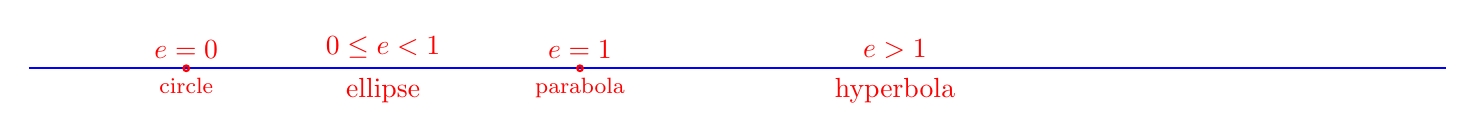
\begin{tikzpicture}%[scale=0.8]
%\draw [help lines] (-10,-1) grid (10,1);
\draw [  thick, blue] (-10,0)--(8,0); 
\draw[red,thick] (-8,0) circle (1pt); 
\node [red,above] at (-8, 0) { $e=0$};
\node [red,below] at (-8, 0) {\footnotesize circle};
%\draw[red,thick] (-3,0) circle (1pt); 
\node [red,above] at (-5.5,0) { $0\leq e <1$};
\node [red,below] at (-5.5, 0) { ellipse};
\draw[red,thick] (-3,0) circle (1pt); 
\node [red,above] at (-3, 0) { $e=1$};
\node [red,below] at (-3, 0) {\footnotesize parabola};
%\draw[red,thick] (-8,0) circle (1pt); 
\node [red,above] at (1, 0) { $e>1$};
\node [red,below] at (1, 0) {hyperbola};
\end{tikzpicture}
\end{equation}

}



\subsection {Intersection of plane with conical  surface}

In this lecture we consider intersections of
planes and surface of cone, conical surface.

 The intersection of plane with conical surface
is an ellipse, a hyperbola, or parabola.
 This justifies why we call
ellipses, hyperbolas and parabola by conic sections. 

  Moreover the orthogonal projection of this 
conic section on the horisontal plane $z=0$ is also 
the conic section, and
 the vertex of the cone is the focus of this conic section
\footnote{Recalling the Kepler law that the planets move in
elliptical orbits with the Sun at one focus one can say
that vertex of the conical surface is a `sun'}.
 
 We  will formulate this Theorem and 
will give its  proof.


     Consider conical surface $M$:

       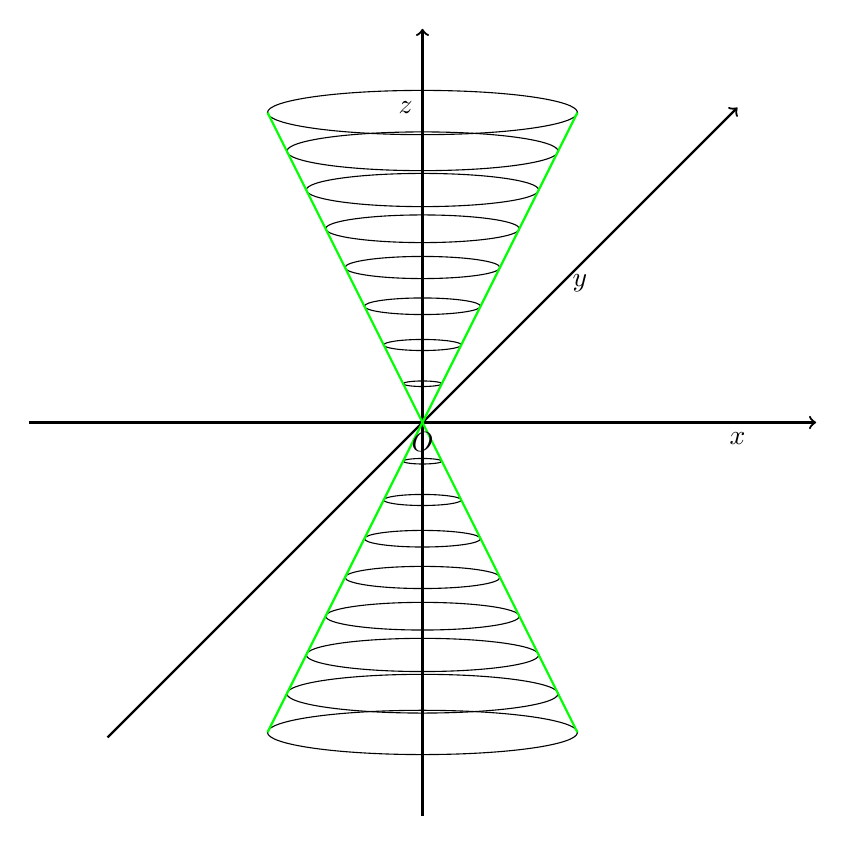
\begin{tikzpicture}
 \draw 
[ <-> , thick] 
(5,0)--(0,0)--(0,5);
\draw 
[ -> , thick] 
(0,0)--(4,4);

\draw 
[ - , thick] 
(-5,0)--(0,0)--(0,-5);
\draw 
[ - , thick] 
(0,0)--(-4,-4);


\draw (0,112pt) ellipse (56pt and 8pt);
\draw (0,98pt) ellipse (49pt and 7pt);
\draw (0,84pt) ellipse (42pt and 6pt);
\draw (0,70pt) ellipse (35pt and 5pt);
\draw (0,56pt) ellipse (28pt and 4pt);
\draw (0,42pt) ellipse (21pt and 3pt);
\draw (0,28pt) ellipse (14pt and 2pt);
\draw (0,14pt) ellipse (7pt and 1pt);

\draw [thick,green] (0,0)--(56pt,112pt);
\draw [thick,green] (0,0)--(-56pt,112pt);

\draw (0,-112pt) ellipse (56pt and 8pt);
\draw (0,-98pt) ellipse (49pt and 7pt);
\draw (0,-84pt) ellipse (42pt and 6pt);
\draw (0,-70pt) ellipse (35pt and 5pt);
\draw (0,-56pt) ellipse (28pt and 4pt);
\draw (0,-42pt) ellipse (21pt and 3pt);
\draw (0,-28pt) ellipse (14pt and 2pt);
\draw (0,-14pt) ellipse (7pt and 1pt);

\draw [thick,green] (0,0)--(56pt,-112pt);
\draw [thick,green] (0,0)--(-56pt,-112pt);


\node [left] at (0,4) {$z$};
\node [below] at (4,0) {$x$};
\node [below] at (2,2) {$y$};
\node [below] at (0,0) {$O$};

%\draw [thick, red,->] (0,0)--(2,3); 
%\node [right] at (1,1.5) {$\r$};
%\node [right] at (2,3) {$A$};

   \end{tikzpicture}

   \begin{equation*}
   M\colon\quad                  
z^2=k^2(x^2+y^2)\,,
\begin{cases}
   x=h\cos\varphi\cr
   x=h\sin\varphi\cr
   z=kh\cr
\end{cases}
  \,,k\not=0,\, (k>0)\,.
\end{equation*}



{\bf Theorem}
{\it 

Let $C$ be a curve which is an intersection of a plane $\alpha$ with
the conical  surface. Let $C_{\rm proj}$ be 
an orthogonal projection of
this curve on the horisontal plane $OXY$.
(We suppose that axis of cone is vertical line.)





\begin{itemize}

\item
   A curve $C$ is a conic section, ellipse, hyperbola or parabola,

\item

    A curve $C_{\rm proj}$ is also conic section:
                           \begin{equation*}
            \begin{cases}
   \hbox {$C$ is an ellpse}\Leftrightarrow\hbox 
 {$C_{\rm proj}$ is an ellpse}\cr
   \hbox {$C$ is a hyperbola}
 \Leftrightarrow\hbox {$C_{\rm proj}$ is a hyperbola}\cr
   \hbox {$C$ is a parabola}\Leftrightarrow
   \hbox {$C$ is a parabola}\cr
          \end{cases}
                           \end{equation*}

\item

    The remarkable property of curve $C_{\rm proj}$ is that
the vertex  of the conical surface is a focus of the conic
section  $C_{\rm proj}$.

\end{itemize}
}

{\bf Remark} We will consider in detail intersection
of planes with upper-sheet of conical surface (see Figure 
\eqref{conicalsurfaceM}). If intersection of
plane $\a$ with  conical
surface is hyperbola, then the intersection with
upper-sheet will be only one branch of hyperbola.



{\bf Remark}
We do not consider degenerate case
if the origin belongs to the plane 
$\a$\footnote{One can see that in this
case the curve $C$ becomes a point or just two lines.}.

\m

  {\tt Proof}

We will consider upper half of conical  surface,
respectively we will consider intersection
of planes with upper-sheet of conical surface.
\footnote{Thus in the case of hyperbola we will come
only to one of branches of hyperbola}:

  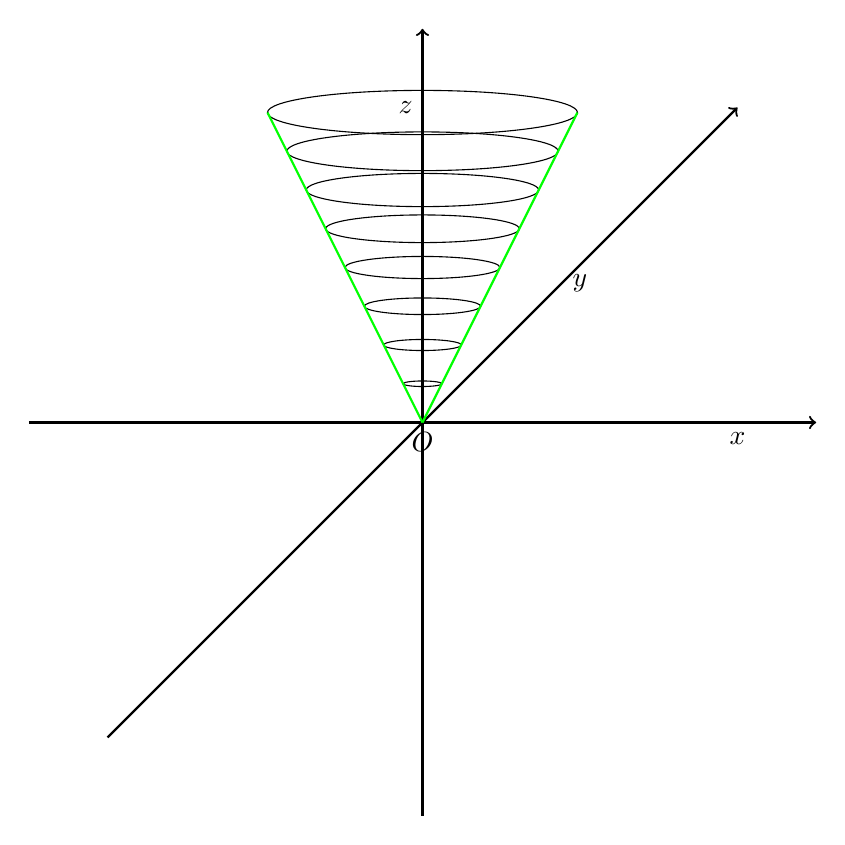
\begin{tikzpicture}
 \draw 
[ <-> , thick] 
(5,0)--(0,0)--(0,5);
\draw 
[ -> , thick] 
(0,0)--(4,4);

\draw 
[ - , thick] 
(-5,0)--(0,0)--(0,-5);
\draw 
[ - , thick] 
(0,0)--(-4,-4);


\draw (0,112pt) ellipse (56pt and 8pt);
\draw (0,98pt) ellipse (49pt and 7pt);
\draw (0,84pt) ellipse (42pt and 6pt);
\draw (0,70pt) ellipse (35pt and 5pt);
\draw (0,56pt) ellipse (28pt and 4pt);
\draw (0,42pt) ellipse (21pt and 3pt);
\draw (0,28pt) ellipse (14pt and 2pt);
\draw (0,14pt) ellipse (7pt and 1pt);

\draw [thick,green] (0,0)--(56pt,112pt);
\draw [thick,green] (0,0)--(-56pt,112pt);

\node [left] at (0,4) {$z$};
\node [below] at (4,0) {$x$};
\node [below] at (2,2) {$y$};
\node [below] at (0,0) {$O$};

%\draw [thick, red,->] (0,0)--(2,3); 
%\node [right] at (1,1.5) {$\r$};
%\node [right] at (2,3) {$A$};

   \end{tikzpicture}
\begin{equation}\label{conicalsurfaceM}
      M\colon\quad               
z^2=k^2(x^2+y^2)\,,\, z>0\,,
 \begin{cases}
   x=h\cos\varphi\cr
   x=h\sin\varphi\cr
   z=kh\cr
\end{cases}\,,h>0
\end{equation}

  Let $\a$ be a plane which does not pass through the origin,

  	 Consider first the simplest case, if
 a plane $\a$ is parallel to the horisontal plane.
            \begin{equation*}
  \begin{cases}
 \a\colon z=H\cr
 M\colon z^2=k^2(x^2+y^2) 
    \end{cases}
   \Leftrightarrow 
   \begin{cases}
            z=H\cr
 x^2+y^2={H^2\over k^2} 
    \end{cases}
  \end{equation*}
Intersection is circle. Its projection on the plane $OXY$
is the circle also, and the vertex of
the conical surface is the centre of this projected
circle.  The centre of the  circle is obviously the focus
of the cicle.-Circle it is the ellipse with 
two coiciding foci.

       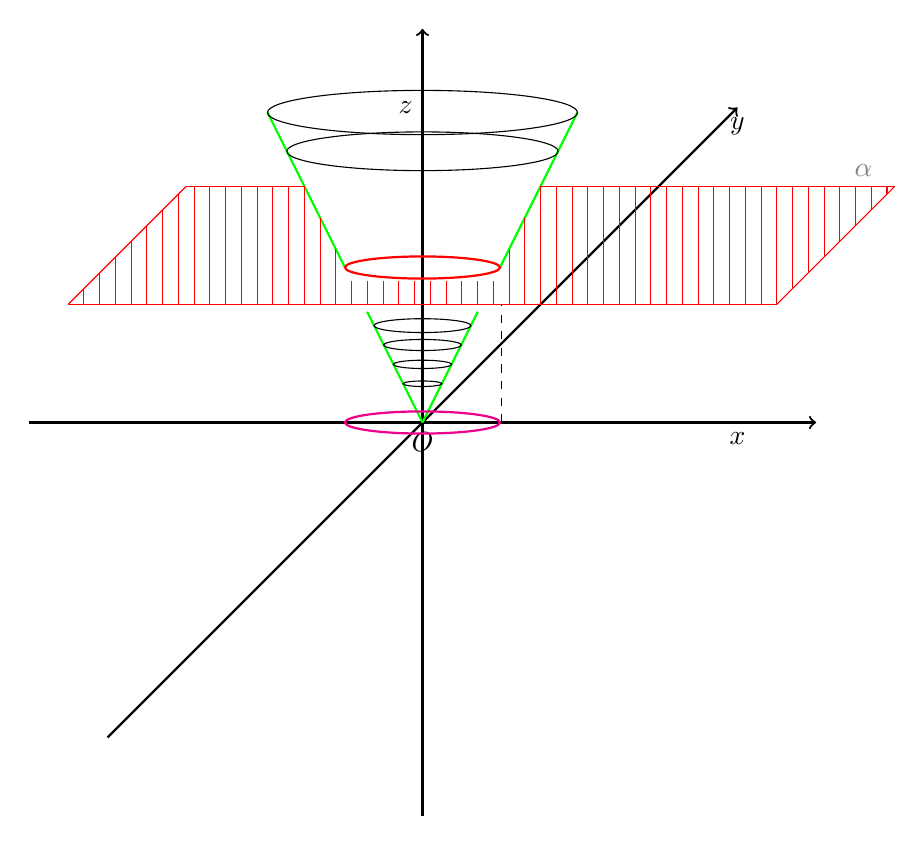
\begin{tikzpicture}
%\draw [help lines] (-6,-1) grid (8,6);
 \draw 
[ <-> , thick] 
(5,0)--(0,0)--(0,5);
\draw 
[ -> , thick] 
(0,0)--(4,4);

\draw 
[ - , thick] 
(-5,0)--(0,0)--(0,-5);
\draw 
[ - , thick] 
(0,0)--(-4,-4);


\draw [thick,green] (0,0)--(20pt, 40pt);
\draw [thick,green] (28pt,56pt)--(56pt,112pt);

\draw [thick,green] (0,0)--(-20pt, 40pt);
\draw [thick,green] (-28pt,56pt)--(-56pt,112pt);





\draw (0,112pt) ellipse (56pt and 8pt);
\draw (0,98pt) ellipse (49pt and 7pt);
\draw [red,thick] (0,56pt) ellipse (28pt and 4pt);
\draw (0,35pt) ellipse (17.5pt and 2.5pt);
\draw (0,28pt) ellipse (14pt and 2pt);
\draw (0,21pt) ellipse (10.5pt and 1.5pt);
\draw (0,14pt) ellipse (7pt and 1pt);


% ramki ploskosti


\draw [red, thin] (-4.5,1.5)--(4.5,1.5);
\draw [red, thin] (-4.5,1.5)--(-3.0,3.0);
\draw [red, thin] (-3.0,3.0)--(-1.5,3.0);
\draw [red, thin] (1.5,3.0)--(6.0,3.0);
\draw [red, thin] (4.5,1.5)--(6.0,3.0);


% shtrikhovka ploskosti
\draw [red,thin] (-4.3,1.5)--(-4.3, 1.7);
\draw [red,thin] (-4.1,1.5)--(-4.1, 1.9);
\draw [red,thin] (-3.9,1.5)--(-3.9, 2.1);
\draw [red,thin] (-3.7,1.5)--(-3.7, 2.3);
\draw [red,thin] (-3.5,1.5)--(-3.5, 2.5);
\draw [red,thin] (-3.3,1.5)--(-3.3, 2.7);
\draw [red,thin] (-3.1,1.5)--(-3.1, 2.9);
\draw [red,thin] (-2.9,1.5)--(-2.9, 3.0);
\draw [red,thin] (-2.7,1.5)--(-2.7, 3.0);
\draw [red,thin] (-2.5,1.5)--(-2.5, 3.0);
\draw [red,thin] (-2.3,1.5)--(-2.3, 3.0);
\draw [red,thin] (-2.1,1.5)--(-2.1, 3.0);
\draw [red,thin] (-1.9,1.5)--(-1.9, 3.0);
\draw [red,thin] (-1.7,1.5)--(-1.7, 3.0);
\draw [red,thin] (-1.5,1.5)--(-1.5, 3.0);
\draw [red,thin] (-1.3,1.5)--(-1.3, 2.6);
\draw [red,thin] (-1.1,1.5)--(-1.1, 2.2);
\draw [red,thin] (-0.9,1.5)--(-0.9, 1.8);

% shtrikhovka ellipsa
\draw [red,thin] (-0.9,1.5)--(-0.9, 1.6);
\draw [red,thin] (-0.7,1.5)--(-0.7, 1.8);
\draw [red,thin] (-0.5,1.5)--(-0.5, 1.8);
\draw [red,thin] (-0.3,1.5)--(-0.3, 1.8);
\draw [red,thin] (-0.1,1.5)--(-0.1, 1.8);
\draw [red,thin] (0.1,1.5)--(0.1, 1.8);
\draw [red,thin] (0.3,1.5)--(0.3, 1.8);
\draw [red,thin] (0.5,1.5)--(0.5, 1.8);
\draw [red,thin] (0.7,1.5)--(0.7, 1.8);



\draw [red,thin] (0.9,1.5)--(0.9, 1.8);
\draw [red,thin] (1.1,1.5)--(1.1, 2.2);
\draw [red,thin] (1.3,1.5)--(1.3, 2.6);
\draw [red,thin] (1.5,1.5)--(1.5, 3.0);
\draw [red,thin] (1.7,1.5)--(1.7, 3.0);
\draw [red,thin] (1.9,1.5)--(1.9, 3.0);
\draw [red,thin] (2.1,1.5)--(2.1, 3.0);
\draw [red,thin] (2.3,1.5)--(2.3, 3.0);
\draw [red,thin] (2.5,1.5)--(2.5, 3.0);
\draw [red,thin] (2.7,1.5)--(2.7, 3.0);
\draw [red,thin] (2.9,1.5)--(2.9, 3.0);
\draw [red,thin] (3.1,1.5)--(3.1, 3.0);
\draw [red,thin] (3.3,1.5)--(3.3, 3.0);
\draw [red,thin] (3.5,1.5)--(3.5, 3.0);
\draw [red,thin] (3.7,1.5)--(3.7, 3.0);
\draw [red,thin] (3.9,1.5)--(3.9, 3.0);
\draw [red,thin] (4.1,1.5)--(4.1, 3.0);
\draw [red,thin] (4.3,1.5)--(4.3, 3.0);
\draw [red,thin] (4.5,1.5)--(4.5, 3.0);
\draw [red,thin] (4.7,1.7)--(4.7, 3.0);
\draw [red,thin] (4.9,1.9)--(4.9, 3.0);
\draw [red,thin] (5.1,2.1)--(5.1, 3.0);
\draw [red,thin] (5.3,2.3)--(5.3, 3.0);
\draw [red,thin] (5.5,2.5)--(5.5, 3.0);
\draw [red,thin] (5.7,2.7)--(5.7, 3.0);
\draw [red,thin] (5.9,2.9)--(5.9, 3.0);
%%%%%%%%%%%%%%%%%%%%%%%%%%%%%%%%%%%%%%%%%
\node [above,gray] at (5.6,3) {$\alpha$};



\node [left] at (0,4) {$z$};
\node [below] at (4,0) {$x$};
\node [below] at (4,4) {$y$};
\node [below] at (0,0) {$O$};


\draw [magenta,thick] (0,0) ellipse (28pt and 4pt);

\draw [dashed] (1,0)--(1,1.5);
   \end{tikzpicture}
 
 \begin{equation*}
                     z^2=k^2(x^2+y^2)\,,\quad k\not=0\,.
\end{equation*}


\bigskip


Consider now a case if plane $\alpha$ is not 
parallel to the plan $OXY$.

In this case ROTATE the space $\E^3$ with respect 
to the axis $OZ$
such that the plane $\a$ after rotation 
becomes parallel to the axis
  $OY$:


 
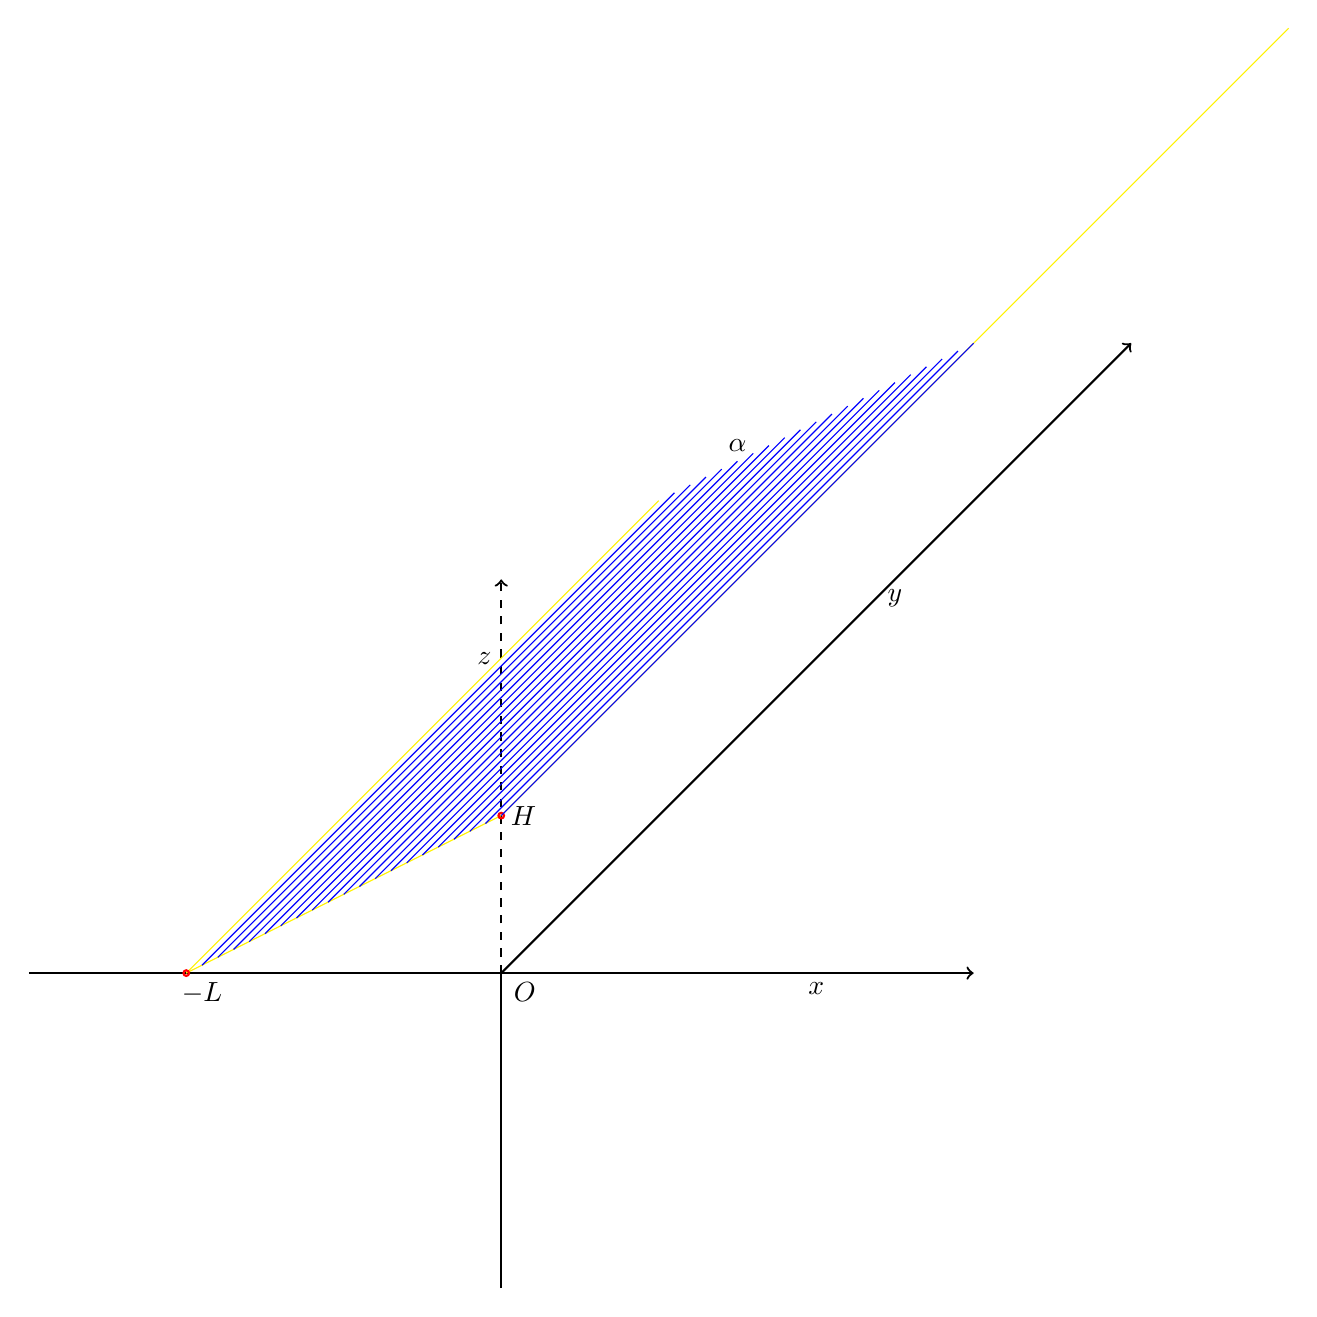
\begin{tikzpicture}
%\draw [help lines] (-5,-1) grid (10,10);
\draw [ -> , thick] (-6,0)--(0,0)--(6,0);
\draw [ - , thick] (0,-4)--(0,0);
\draw [ -> , thick, dashed] (0,0)--(0,5);
\draw [ -> , thick] (0,0)--(8,8);

\node [left] at (0,4) {$z$};
\node [below] at (4,0) {$x$};
\node [below] at (5,5) {$y$};
\node [below] at (0.3,0) {$O$};

\draw [yellow] (-4,0)--(0,2);
\draw [yellow] (0,2)--(10,12);
\draw [yellow] (-4,0)--(2,6);

\draw [red, thick] (-4,0) circle (1pt);
\node [below] at (-3.8,0) {$-L$};
\draw [red, thick] (0,2) circle (1pt);
\node [right] at (0,2) {$H$};
\node [above] at (3,6.5) {$\alpha$};

%  shtrikhovka:

\draw [thin, blue] (-3.8,0.1)--(2.2,6.1);
\draw [thin, blue] (-3.6,0.2)--(2.4,6.2);
\draw [thin, blue] (-3.4,0.3)--(2.6,6.3);
\draw [thin, blue] (-3.2,0.4)--(2.8,6.4);
\draw [thin, blue] (-3.0,0.5)--(3.0,6.5);
\draw [thin, blue] (-2.8,0.6)--(3.2,6.6);
\draw [thin, blue] (-2.6,0.7)--(3.4,6.7);
\draw [thin, blue] (-2.4,0.8)--(3.6,6.8);
\draw [thin, blue] (-2.2,0.9)--(3.8,6.9);
\draw [thin, blue] (-2.0,1.0)--(4.0,7.0);
\draw [thin, blue] (-1.8,1.1)--(4.2,7.1);
\draw [thin, blue] (-1.6,1.2)--(4.4,7.2);
\draw [thin, blue] (-1.4,1.3)--(4.6,7.3);
\draw [thin, blue] (-1.2,1.4)--(4.8,7.4);
\draw [thin, blue] (-1.0,1.5)--(5.0,7.5);
\draw [thin, blue] (-0.8,1.6)--(5.2,7.6);
\draw [thin, blue] (-0.6,1.7)--(5.4,7.7);
\draw [thin, blue] (-0.4,1.8)--(5.6,7.8);
\draw [thin, blue] (-0.2,1.9)--(5.8,7.9);
\draw [thin, blue] (-0.0,2.0)--(6.0,8.0);



\end{tikzpicture}
\begin{equation}\label{planealpha}
\hbox{equation of the plane $\a$}\,, \quad {z\over H}=1+{x\over L}\,.
\end{equation}
The plane $\a$ intersects the axis $OZ$ at the point $(0,0,H)$,
and it intersects the axis $OX$ at the point $(O,O,-L)$.


(Recall that the plane $\a$ is not parallel to the plane $OXY$).

       Equation of the plane $\a$  is
                     \begin{equation}\label{planealpha}
    {z\over H}=1+{x\over L}\,. 
                     \end{equation}
(Indeed we see that if $x=y=0$ then $z=H$ and if $y=z=0$ then $x=-L$.)

{\bf Remark} {\footnotesize   The case when a plane $\a$
which is not parallel to $OXY$ and passes through the origin is degenerate case.
  In this case plane $\a$ intersects with conical surface by
point, vertex, or two lines.  We do not consider this degenerate case.}



  Now analyze the intersection of the plane $\a$ with conical
surface $M$.   We have:
          \begin{equation*}
\underbrace{\a\times M}_{\hbox 
{{\footnotesize intersection of the plane $\a$
 with conical surface $M$}}}
\colon\quad
      \begin{cases}
  {z\over H}=1+{x\over L}\cr
      k^2x^2+k^2y^2-z^2=0\cr    
      \end{cases}
     \Leftrightarrow
          \end{equation*}
     \begin{equation*} 
      \begin{cases}
      z=H\left(1+{x\over L}\right)\cr
      k^2x^2+k^2y^2-z^2=0\cr    
      \end{cases}
      \Leftrightarrow
      \begin{cases}
      z=H\left(1+{x\over L}\right)\cr
      k^2x^2+k^2y^2-
   \left(H\left(1+{x\over L}\right)\right)^2=0\cr    
      \end{cases}\,.
     \end{equation*} 
Denote this intersection by $C$. This equation defines
locus of the points in $\E^3$, the curve
$C$ which is the intersection of conical surface $M$
and the plane $\a$:
           \begin{equation}\label{conicsectionequation1}
C=\a\times M\colon \quad \begin{cases}
      z=H\left(1+{x\over L}\right)\cr
      k^2x^2+k^2y^2-
   \left(H\left(1+{x\over L}\right)\right)^2=0\cr    
      \end{cases}\,.
           \end{equation}
Denote by $C_{\rm proj}$ an orthogonal projection of this curve
on the horizontal plane $z=0$.

We see for orthogonal projection that
                \begin{equation*}
                    \begin{matrix}
&(x,y,z)&-\hbox {a point on the curve $C$ which is a curve in $\E^3$}\cr
       &\downarrow\cr 
&(x,y,0)&-\hbox {orthogonal projection of this point,
           a point on the curve $C_{\rm proj}$, a curve in $\E^2$}\cr
                   \end{matrix} 
             \end{equation*}
Hence
            \begin{equation*}\label{projofconicsectionequation1}
C_{\rm proj}\colon\quad \begin{cases}
      z=0\cr
      k^2x^2+k^2y^2-
   \left(H\left(1+{x\over L}\right)\right)^2=0\cr    
      \end{cases}
           \end{equation*}
i.e. the orthogonal projection of the curve $C$
defined by equation \eqref{conicsectionequation1}
is the curve $C_{\rm proj}$ defined in the plane $\E^2$ defined
by equation
             \begin{equation}\label{projofconicsectionequation1}
C_{\rm proj}\colon k^2x^2+k^2y^2-
   \left(H\left(1+{x\over L}\right)\right)^2=0\,,\quad
(z=0)\,.
           \end{equation}
Here  $\E^2$ is the horizontal plane $z=0$.


    We see that equation \eqref{conicsectionequation1} 
defines conic section 
$C=\a\times M$ (intersection of plane $\a$ 
with conical surface 
$M$)
and equation \eqref{projofconicsectionequation1} 
defines a curve $C_{\rm proj}$,
 the curve which is the
orthogonal projection of the curve $C$ on the plane $z=0$
(see further Figure 
\eqref{projectionofconiconthehorizontalplane}.)

   Our plan is following. 
We first prove that curve
$C_\proj$ is a conic surface,
i.e. it is an ellipse, or hyperbola or parabola.
Then we will prove that the vertex of the conical surface
$M$ is a focus of the  conic section $C_{\rm proj}$,
and finally we will show that initial curve
$C$ is also a conic section. 



Now begin the proof.
  The proof of the fact that $C_\proj$ is a conic section
will be done in two different ways. 
We will perform straightforward calculations 
in Cartesian coordinates then we will come to
the same result   
or much shorter in `one-line' caluclations
 in polar coordinates.
It is useful to see how these two methods work.



Let $C_{\rm proj}$ be a curve
in $\E^2$ defined by  
equation\eqref{projofconicsectionequation1}.
Denote by 
      \begin{equation*}
     \delta=k^2-{H^2\over L^2}\,.
           \end{equation*}
Show that the curve $C_\proj$ is an ellipse if $\delta>0$,
 it is
hyperbola if $\delta<0$, and it is parabola
if $\delta=0$.

We have   \begin{equation*}
C_{\rm proj}\colon k^2x^2+k^2y^2-
   \left(H\left(1+{x\over L}\right)\right)^2=0\Leftrightarrow
   \underbrace{\left(k^2-{H^2\over L^2}\right)}_{\delta}
         x^2-{2H^2\over L}x+k^2y^2-H^2=0\,.
           \end{equation*}
We come to  
   \begin{equation*}
C_{\rm proj}\colon \quad
 \delta x^2-{2H^2\over L}x+k^2y^2-H^2=0\,,\quad (z=0)\,.
           \end{equation*}      
First, consider the case $\delta=0$.
In this case $C_{\rm proj}$ is a parabola:
       \begin{equation*}
\delta=0\,, \quad
C_{\rm proj}\colon \quad -{2H^2\over L}x+k^2y^2-H^2=0
\Leftrightarrow
             y^2={2H^2\over k^2L}y^2+{H^2\over 2}=
          {2H^2\over k^2L}\left(x+{L\over 2}\right)\,.
           \end{equation*}      
One can reduce this parabola to canonical
form $y^2=2px$ (see analytical definition of
parabola \eqref{analytparabola}).
 Under translation  $x'=x+{L\over 2}$ we come to
new Cartesian coordinates such that
        \begin{equation}\label{conditionforparabola}
C_{\rm proj}\colon 
      y^2=2px'\,,\quad
          {\rm where}\,\, p= {H^2\over k^2L}\,,\,
{\rm if}\, \delta=k^2-{H^2\over L^2}=0\,.
           \end{equation}  
Note that condition $\delta=0$ implies that 
     \begin{equation}\label{noteforparabola1}
     p= {H^2\over k^2L}={H\over k}=L\,.
            \end{equation}
(We suppose that $k>0$.)

We have proved that the curve $C_{\rm proj}$ in $\E^2$
is a parabola if $\delta=0$.

\m


Now consider the case if $\delta\not=0$. In this case:
  \begin{equation*}
C_{\rm proj}\colon k^2x^2+k^2y^2-
   \left(H\left(1+{x\over L}\right)\right)^2=0\Leftrightarrow
   \underbrace{\left(k^2-{H^2\over L^2}\right)}_{\delta\not=0}
         x^2-{2H^2\over L}x+k^2y^2-H^2=0\,.
           \end{equation*}
Hence we have
         \begin{equation}\label{lemmacalculations1}
C_{\rm proj}\colon \delta x^2-{2H^2\over L}x+k^2y^2-H^2=
  \delta\left(x-{H^2\over L\delta}\right)^2+k^2y^2-
    H^2\left(1+{H^2\over \delta L^2}\right)=0\,.
           \end{equation}
We see that in Cartesian coordinates 
       \begin{equation}\label{cartesiancoordinates2}
        \begin{cases}x'=x-{H^2\over L\delta}\cr y'=y\cr
     \end{cases}
         \end{equation}
the curve $C_{\rm proj}$ is ellipse if $\delta>0$
and it is  hyperbola if $\delta<0$.



Indeed in the case if $\delta>0$ we have from
equation \eqref{lemmacalculations1} that
              \begin{equation*}
  \delta x'\,^2+k^2y'\,^2=H'^2\Leftrightarrow
    \left({x'\over a}\right)^2+\left({y'\over b}\right)^2=1\,, 
              \end{equation*} 
where $x',y'$ are Cartesian coordinates
\eqref{cartesiancoordinates2}, and
we denote
           \begin{equation}\label{notations4}
          H'=H\sqrt{1+{H^2\over \delta L^2}}\,,\quad
     a={H'\over \sqrt \delta}\,,\quad
         b={H'\over k}\,,\, {\rm if}\,\,
\delta=k^2-{H^2\over L^2}>0\,.
            \end{equation}
Note that conditon $a\geq b$ is fullfilled:
Indeed
$a={H'\over \sqrt \delta}>{H'\over k }=b$
since $\delta<k^2$, ($\delta>0$).
 
We have constructed Cartesian coordinates 
$(x',y')$ such that
in these coordinates the curve $C_{\rm proj}$ 
is defined by canonical equation 
    $\left({x'\over a}\right)^2+\left({y'\over b}\right)^2=1$,
with  $a\geq b$, hence it is an ellipse
according analytica definition of ellipse
(see equation \eqref{analytell} in
subsection  \ref{analyticdefinitions}).

 We have proved,
that  
the curve $C_{\rm proj}$ in $\E^2$
is an ellipse if $\delta>0$.

\m

{\footnotesize  
In the case if $\delta<0$ we do analogous calculations.
We have that in this case  equation
\eqref{lemmacalculations1} implies that
the curve $C_{\proj}$ has the appearance 
   \begin{equation*}
C_{\rm proj} \colon\quad \delta x'\,^2+k^2y'\,^2=
H'\,^2\,,\quad\left( H'^2=
H^2\left(1+{H^2\over \delta L^2}\right)\,,\delta<0, 
\delta<0\right)
   \end{equation*}
in Cartesian coordinates
$(x',y')$.  Hence 
                     \begin{equation}\label{calculations4}
        {y'^2\over H'^2/k^2}
        -{x'^2\over H'^2/|\delta|}=1\,, 
\delta=k^2-{H^2\over L^2}<0)\,.
                    \end{equation}
Swapping these Cartesian coordinates 
$x'\leftrightarrow y'$  we will come to 
Cartesian coordinates   
     \begin{equation*}
        \begin{cases}x{''}=y'=y\cr
        y{''}=x' =x+{H^2\over L\delta}\cr 
     \end{cases}
         \end{equation*}
such that in these Cartesian coordinates
equation \eqref{calculations4} becomes
 canonical
equation of hyperbola
            $$
      \left({x{''}\over  a}\right)^2
        -
    \left( {y{''}\over  b}\right)^2=1\,,
         $$
with parameters $a,b$ such that $a,b>0$ and
        $$
     a^2={H'^2\over k^2}\,,
\quad  b^2={H'^2\over -\delta} \,,(\delta<0)\,.
     $$
(See equation 
\eqref{analythyp} in subsection
\ref{analyticdefinitions}). 
The curve $C_{\rm proj}$ in $\E^2$
is a hyperbola.



}

We proved, that the curve $C_{\rm proj}$
in the horizontal plane defined by equation
 \eqref{projofconicsectionequation1}
is ellipse or hyperbola or parabola.

  \m

Now prove that a focus of the curve 
$C_\proj$ is the vertex of the cone.
Vertex of cone is the  origin $x=y=0$
of the horizontal plane $\E^2$.
We have to prove that for curve defined by equation
\eqref{projofconicsectionequation1} 
the origin $x=y=0$
is a focus.

  Consider on horizontal plane
$z=0$ polar coordinates 
$(r,\varphi)\colon
\begin{cases}
x=r\cos\varphi\cr
y=r\sin\varphi\cr
\end{cases}$. We see that $r=\sqrt{x^2+y^2}$
and $x=r\cos\varphi$. We have from equation
\eqref{projofconicsectionequation1}:
        \begin{equation*}
k\sqrt{x^2+y^2}=kr=H\left(1-{x\over L}\right)=
H(1-{r\over L}\cos\varphi)\,,
        \end{equation*}
i.e.
        \begin{equation*}
r={H\over k-{H\over L}\cos\varphi}={p\over 1-e\cos\varphi}\,,
\quad {\rm where}\,\, p={H\over k}\,\, {\rm and}\,\,
e={H\over L}\,.
        \end{equation*}

 This equation implies that 
the curve $C_\proj$ is conic section and
the origin is a focus of $C$
(see subsection \eqref{conicsectionsinpolarcoordinates}).

If eccentricity parameter $e={H\over k}=1$ it is a parabola:
compare with condition 
$\delta=k^2-{H^2\over L^2}=0$)  
in \eqref{conditionforparabola};
if eccentricity parameter $e={H\over k}<1$ 
it is ellipse (compare with condition 
$\delta=k^2-{H^2\over L^2}>0$)
in \eqref{notations4}
and
if $e={H\over k}>1$ it is hyperbola 
(compare with condition 
$\delta=k^2-{H^2\over L^2}<0$)
in\eqref{calculations4}.
(We suppose that $k,H,L>0$,)

\m


We proved that projection of the curve
$C$, the curve $C_\proj$  
defined by equation \eqref{projofconicsectionequation1}
on the horizontal plane 
is ellipse, hyperbola or parabola, and vertex of the conical
surface is a focus of this conic.

To finish the proof of the Theorem we will prove 
that curve $C$,  defined by equation \eqref{conicsectionequation1}
is itself conic section also. This  follows
immediately from considerations presented in 
Figure \eqref{projectionofconiconthehorizontalplane}.



% orthogonal projecton of $C$ on $C_{\rm proj}$ 



\begin{tikzpicture}

%\draw [help lines] (-8,-1) grid (10,16);

\draw [red] (8, 0)--(-7,0);
\draw [red] (8, 0)--(7,5);
\draw [red] (7, 5)--(-8,5);
\draw [red] (-7, 0)--(-8,5);

\draw [gray] (-7,0)--(3,15);
\draw [gray] (3,15)--(2,20);
\draw [gray] (-8,5)--(2,20);
\draw [green,thick] (-6,3)--(-7.6,3)--(-6,5.4);
\draw  [blue] (-6.5,3) arc 
[radius=1, start angle=0, end angle=60];
\node [left] at  (-6.7,3.5) {$\theta$};


\draw  [magenta] (-2,3) ellipse (3 and 0.8);
\draw [->, thick, brown] (-5.2,3)--(1.4,3);
\node [below] at (0,3) {$x$};
\draw [->, thick, brown] (-1.8,2)--(-2.2,4);
\node [left] at (-2.2,4) {$y$};




% for $P_1$
\draw  [dashed]  (1,3)--(1,15);
\draw [yellow, thick] (1,3) circle (1pt);
\node [below] at (1,3) {$P_{1\rm proj}$};
\draw [yellow, thick] (1,15) circle (1pt);
\node [below] at (1,15) {$P_1$};



% for $P_2$
\draw  [dashed]  (0,2.3)--(0,12.3);
\draw [yellow, thick] (0,2.3) circle (1pt);
\node [below] at (0,2.3) {$P_{2\rm proj}$};
\draw [yellow, thick] (0,10.8) circle (1pt);
\node [below] at (0,10.8) {$P_2$};



% for $P_3$
\draw  [dashed]  (-2,2.2)--(-2,8.0);
\draw [yellow, thick] (-2,2.2) circle (1pt);
\node [below] at (-2,2.2) {$P_{3\rm proj}$};
\draw [yellow, thick] (-2,8.0) circle (1pt);
\node [below] at (-2,9.0) {$P_3$};

% for $P_4$
\draw  [dashed]  (-4,2.3)--(-4,5.8);
\draw [yellow, thick] (-4,2.3) circle (1pt);
\node [below] at (-4,2.3) {$P_{4\rm proj}$};
\draw [yellow, thick] (-4,6.2) circle (1pt);
\node [below] at (-4,6.2) {$P_4$};

% for $P_5$
\draw  [dashed]  (-5,3)--(-5,6);
\draw [yellow, thick] (-5,3) circle (1pt);
\node [below] at (-5,3) {$P_{5\rm proj}$};
\draw [yellow, thick] (-5,6) circle (1pt);
\node [below] at (-5,6) {$P_5$};

% C ellipse major axis

%\draw [->, thick, red] (-5.2,3)--(1.4,3);
\draw [->,thick,red ] (-5.2,5.7)--(1.4,15.6);
\node [below] at (0,13.3) {$\tilde x$};

% C ellipse minor axis

\draw [->, thick, red] (-1.8,8)--(-2.2,12.4);
\node [left] at (-2,11) {$\tilde y$};


% Lecala for ellipse  C
% Izmenenija
\draw [very thick,blue] (-5,6) to [out=0, in=230] (-2,8);
\draw [very thick,blue] (-2,8) to [out=50, in=235] (0,10.8);
\draw [very thick,blue] (0,10.8) to [out=60, in=290] (1,15);


% lecales for points reflected with respect to axis $\tilde x$

\draw [very thick,blue] (-5,6) to [out=90, in=235] (-2,12.3);
\draw [very thick,blue] (-2,12.3) to [out=57, in=180] (1,15);
%\draw [very thick,blue] (-2,8) to [out=50, in=235] (0,10.8);
%\draw [very thick,blue] (0,10.8) to [out=60, in=290] (1,15);




\end{tikzpicture}
\begin{equation}
\label{projectionofconiconthehorizontalplane}
%     \tilde x={x\over\cos\theta}\,,\quad
 %    \tilde y=y\,.
\end{equation}




Recall that the curve $C$ is the intersection of
the plane $\a\colon {x\over H}+{y\over L}=1$
(see \eqref{conicsectionequation1})  with coniccal  surface  $M$.

 Let $\theta$ be an angle between the plane $\a$ and horizontal
plane $OXY$ (see Figure \eqref{projectionofconiconthehorizontalplane}),
 then
            $$
      {\rm tan\,}\theta={H\over L}\,.
            $$
Thus if $x,y$ are Cartesian coordinates on the plane
  $OXY$ then one can choose on the plane $\alpha$
Cartesian coordinates $(\tilde x,\tilde y)$ such that 
      \begin{equation}\label{cartesiancoordinatesontheplane}
       \tilde x={x\over\cos\theta}\,,\quad
       \tilde y=y\,.
     \end{equation} 
Recall that the orthogonal projection $C_{\rm proj}$
of the curve $C$ is defined in the horizontal plane $z=0$ by
the equation 
  \begin{equation}\label{projectionofconicsection4}
C_{\rm proj}\colon k^2x^2+k^2y^2-
   \left(H\left(1-{x\over L}\right)\right)^2=0\,, (z=0)\,.
           \end{equation}
(see \eqref{projofconicsectionequation1}.)


Hence in Cartesian coordinates $(\t x, \t y)$
\eqref{cartesiancoordinatesontheplane} in the plane $\a$,
the 
curve $C$ has the same appearance as a curve $C_\proj$
in Cartesian coordinates $(x,y)$:
                     $$
C\colon k^2{\tilde x}^2+k^2{\tilde y}^2-
   \left(H\left(1-{{\tilde x}\over L}\right)\right)^2=0\,.
           $$
   (The curve $C$ in the plane $\a$ is defined
by the same equations that the curve $C$ in the horisontal 
plane $z=0$, just we have to 
change $x\mapsto \tilde x, y\mapsto y$.)

This implies that curve $C$ is conic section also,
it is an ellipse if $C_\proj$ is an ellipse,
it is a hyperbola if $C_\proj$ is a hyperbola,
it is parabola  if $C_\proj$ is an ellipse,

E.g. if $C_{\proj}$ is ellipse, then
in Cartesian coordinates 
$\begin{cases}x'=x-{H^2\over L\delta}\cr y'=y\cr
     \end{cases}$ it is defined by canonical expression
                $$
\left(x'\over a\right)^2+
\left(y'\over b\right)^2=1
                 $$
(see equations \eqref{cartesiancoordinates2} and 
\eqref{notations4}).   Hence the curve $C$
 which is in the plane $\a$ has the same appearance
                $$
\left(\tilde {x'}\over a\right)^2+
\left({\tilde y'}\over b\right)^2=1\,,
              \, {\rm with}\,
 \begin{cases}
   {\tilde x'}={x'\over \cos\theta}
  % {x-{H^2\over L\delta}\over \cos\theta}
         \cr 
 {\tilde y'}=  y'
       \cr
     \end{cases}
              $$
%{\footnotesize  We know that vertex of cone is one of foci of 
%the curve $C_\proj$. What about the curve $C$?
%One can show that intersection of curve $C$ with horisontal plane
%is directrix of this conic section. }

 \m

    \centerline {\bf Resum\'e}
                 \begin{equation*}
                \begin{matrix}
 \hbox {plane $\alpha$}   &
 \hbox {horizontal plane}  \cr
   {x\over L}+{y\over H}=1 & z=0\cr
    \hbox {$C$--intersection of plane $\a$}  &
    \hbox {$C_{\rm proj}$--orthogonal projection of} \cr
  \hbox{with conical surface $M$}
         & \hbox{$C$ on the horizontal plane}\cr
    \hbox{Cartesian coordinates $\tilde x,\tilde y$} &
    \hbox{Cartesian coordinates $x,y$}\cr
       \tilde x={x\over \cos\theta}\,,
         \tilde y=y\,,\,   &  {\rm tan}\theta={H\over L}\cr
              \end{matrix} 
                 \end{equation*}




\subsection{Basic elements of Projective Geometry}



%\end{document} % 20 April 2018

Projective geometry has very interesting history
\footnote{just key words:\begin{itemize}

\item  Pappus of Alexandria (III-rd century)

\item Johannes Kepler  (1571---1630)

\item     Gerard Desargus (1571---1630)

\item     Projective Geometry in painting

\end{itemize}     

}

\subsubsection {Projective line $\R\bf P$}

               \begin{equation*}
\hbox {Projective line}\,\, \underbrace{\R}_
      {\hbox{\footnotesize usual line}} =\R\cup 
       \underbrace\{\infty\}_{\hbox{\footnotesize point at infinity}}
              \end{equation*}
In other words

  Projective line $=$ usual line 
completed by a point at infinity.


\bigskip

     \centerline  {\Large Model}

\m



    \begin{tikzpicture}
   \draw       [->] (-8,0)--(0,0)--(8,0); 
   \draw       [->] (0,-3)--(0,0)--(0,4); 
 \node [below] at (5,0)   {$x$};    
 \node  [right] at (0,3) {$y$};    
\draw [red,thick] (-6,2)--(0,2)--(6,2);
\node [below] at (0,2) {$y=1$};
\node [green] at (0,0) {$O$};


% affine points on the projective line 

\draw [green]  (-4,2) circle (1pt);
\draw  [green](-2,2) circle (1pt);
\draw [green]  (-3,2) circle (1pt);
\draw [green] (1,2) circle (1pt);
\draw [green] (2,2) circle (1pt);
\draw [green]  (5,2) circle (1pt);

% lines through origin


\draw [gray] (2,-1)--(-6,3);
\draw [gray] (3,-3)--(-4,4);
\draw [gray] (3,-2)--(-6,4);
\draw [gray] (-1,-2)--(2,4);
\draw [gray] (-2,-2)--(5,5);
\draw [gray] (-5,-2)--(7.5,3);
\draw [gray] (-1,-0.1)--(3,0.3);
\draw [gray] (-1,-0.05)--(4,0.2);



\end{tikzpicture} 
    \begin{equation*}
     \end{equation*} 

\def\P {{\bf P}}

    \begin{equation*}
 \R\P^1=\{\hbox {set of lines in $\R^2$ passing through the origin}\}=
\{l\colon {\bf 0}\in l\}\,.
     \end{equation*} 

(In our notations $\R\P$ and $\R\P^1$ will be the same)

 \m


{\tt `Point'  of $\R\P$  $=$ line in $\R^2$ passing through the 
origin} 

\m

Every line passing through the origin except the
line $y=0$ intersects the line $y=1$.
Hence all the points of $\R\P$ except the
point which corresponds  to  the line $y=1$
 can be viewed as usual  points at the line $y=1$. 

We call a `point' on $\R\P$ a {\it finite } point (or {\it visible}
point  or {\it proper} point) if it corresponds to the line which 
intersects the line $y=1$,
i.e. the line which is not parallel to the line $y=1$.

We call the `point' on $\R\P$ a {\it point at the infinity}
(or {\it improper} point, or {\it invisible} point)
if it corresponds to the line $y=0$., i.e. the
line which is parallel to the line $y=1$.
 
    \begin{equation*}
     \begin{matrix}
    \hbox {set of lines in $\R^2$}     & & \hbox {set of lines in $\R^2$} 
               & & \hbox {the line}\cr
    \hbox {passing through}     & & \hbox {passing through} 
               & & \hbox {which goes }\cr
    \hbox {the origin}     &= & \hbox {the origin and which } 
               &\cup & \hbox {along $OX$ axis}\cr
    \hbox {}     & & \hbox {intersect} 
               & & \hbox {}\cr
    \hbox {}     & & \hbox {the line $y=1$} 
               & & \hbox {}\cr
    \hbox{all points }     &= & \hbox{finite points of $\R\P$,} 
             &\cup & \hbox{the point at infinity}\cr
     {\rm of}\,\R\P   & {}  &\hbox {(i.e. points of $\R$)} & {} & \{\infty\}\cr  
     \end{matrix}
    \end{equation*}

   \bigskip

We have that

  \begin{equation*}
   \begin{matrix} 
     \hbox {line $l$ which }  & \hbox{a  point}\cr
     \hbox {intersects the line $y=1$}  & 
               \hbox{at the line $y=1$}\cr
           &  \cr
     \hbox {line $l$ which}  & 
               \hbox{}\cr
     \hbox {is parall. to the  line $y=1$}  & 
               \hbox{point at infinity}\cr
   \end{matrix}
     \end{equation*} 

\subsubsection {Homogeneous and affine coordinates on $\R\P$}



    \begin{tikzpicture}
   \draw       [->] (-8,0)--(0,0)--(8,0); 
   \draw       [->] (0,-3)--(0,0)--(0,4); 
 \node [below] at (5,0)   {$x$};    
 \node  [right] at (0,3) {$y$};    
\draw [red,thick] (-6,2)--(0,2)--(6,2);
\node [below] at (0,2) {$y=1$};

\draw [ thick] (3,4) circle (1.5pt);
\draw [ thick] (4.5,6) circle (1.5pt);
\draw [ thick] (0.75,1) circle (1.5pt);
\draw [ thick] (-0.375,-0.5) circle (1.5pt);
\draw [ thick] (3,4) circle (1.5pt);
\draw [ thick] (3,4) circle (1.5pt);
\draw [ thick] (3,4) circle (1.5pt);
\draw [ thick] (3,4) circle (1.5pt);
\draw (-3,-4)--(3.3,4.4);
\draw [dashed] (3.3,4.4)--(6,8);
\draw [above, green,thick] (1.5,2) circle (1.5pt);
\node [left] at (1.5,2)  {$A$};

\end{tikzpicture} 
    \begin{equation*}
     \end{equation*} 



Take an arbitrary point $\begin{pmatrix}a\cr b\cr\end{pmatrix}$ 
on the plane $\E^2$
which does not conicide with the origin ($a\not=0$ or $b\not=0$).
 This point defines a line, passing through the origin
            \begin{equation*}
 \hbox {a point $\begin{pmatrix}a\cr b\cr\end{pmatrix}$ 
defines a line}\,\quad
      \begin{cases} x=at\cr y=bt\cr\end{cases}
        \qquad \hbox {if $a\not=0$ or $b\not=0$}\,.
             \end{equation*}
We denote by $[a:b]$ the line passing through the origin 
and the point
$\begin{pmatrix}a\cr b\cr\end{pmatrix}$.

Why this notation? 
Because for every parameter $\lambda$ such that $\lambda\not=0$,
the point  $\begin{pmatrix}a\cr b\cr\end{pmatrix}$
and the point $\begin{pmatrix}\lambda a\cr \lambda b\cr\end{pmatrix}$
define the same line:
              $$
    [a:b]=[\lambda a:\lambda b]\,,\,\,(\lambda\not=0)\,.
              $$
     
\centerline{
Set of lines passing through the origin $=$ Set of points of $\R\P$}


\smallskip


{\bf Definition}
One can consider  $[a:b]$ as
 coordinates of `points' on projective line $\R\P$  
(We suppose that $a$ and $b$ are not simultaneously equal to zero.)
These coordinates are called {\it homogeneous} coordinates.\\
Coordinates  $[a:b]$ and $[\lambda a:\lambda b]$,
($a\not=0$ or $b\not=0$, and $\lambda\not=0$) define the same `point'
on $\R\P$ $=$ line
      $\begin{cases} x=at\cr y=bt\cr\end{cases}$ in $\E^2$
passing through the origin.

\smallskip

  Let $A$ be an arbitrary point on $\R\P$
with homogeneous coordinates $[x_A:y_A]$,  $A=[x_A:y_A]$.

The `point' $A$ on $\R\P^1$ is represented by the line
$l_A\colon 
\begin{cases} x=x_At\cr y=y_At\cr\end{cases}$.

Now suppose that condition
     \begin{equation}\label{noatinfinity}
           y_A\not=0\,.
     \end{equation}
is obeyed.

In this case the line $l_A$ intersects
the line $y=1$ at the point $u_A={x_A\over y_A}$.
  
 In the case if condition \eqref{noatinfinity}
is not obeyed, i.e. line $l_A$ is parallel to the line $y=1$, then
the `point' $A$ is not a finite point, it is a point
at infinity.

\smallskip

   {\bf Definition}  Let $A=[x_A;y_A]$ be a finite point
at the projective line $\R\P$, i.e. $y_A\not=0$.
 One can consider
{\it affine coordinate} $u_A$ of this point:
     \begin{equation}\label{affinecoordinate}
         u_A={x\over y}
             \end{equation}

If $A$ is not  a finite  point i.e. $A$ is a point
at infinity, then  affine coordinate is not well-defined.
With some abuse of language we say sometimes
that  \begin{equation}\label{affinecoordinate1}
         u_A=\infty\,,\quad {\rm if}\,\, y_A=0\,.
             \end{equation}

       \begin{equation*}
        \begin{matrix}
  \underbrace{ [x:y]}_{\hbox {\footnotesize homogeneous coordinates}} 
      \longrightarrow  
\underbrace{u={x\over y}}_{\hbox{\footnotesize affine coordinate}}\cr
       \end{matrix}
      \end{equation*}

\smallskip

{\bf Example}

    \begin{tikzpicture}
   \draw       [->] (-8,0)--(0,0)--(8,0); 
   \draw       [->] (0,-3)--(0,0)--(0,4); 
 \node [below] at (5,0)   {$x$};    
 \node  [right] at (0,4) {$y$};    
\draw [red,thick] (-6,2)--(0,2)--(6,2);
\node [below] at (0,2) {$y=1$};

\draw [ thick] (8,4) circle (1.5pt);
\node [thick,left] at (8,4) {$[8:4]$};  
\draw [ thick] (6,3) circle (1.5pt);
\node [thick,left] at (6,3) {$[6:3]$};  
\draw [ thick] (-5,-2.5) circle (1.5pt);
\draw (-6,-3)--(6.6,3.3);
\draw [dashed] (6.6,3.3)--(8,4);
\draw [above, green,thick] (4,2) circle (1.5pt);
\node [left] at (4,2)  {$P$};

\end{tikzpicture} 
    \begin{equation*}
     \end{equation*} 


Consider a point $P$ on projective line $\R\P^1$
with homogeneous coordinate $[4:2]$,
$P=[4:2]$.   The line $l_P$ which represents this point
is 
$l_P\colon 
\begin{cases} x=4t\cr y=2t\cr\end{cases}$
This line intersects the line $y=1$ at the point
$(2,1)$. Homogeneous coordinates of the same but one point 
may have different appearance. We see that 

          $$
[4;2]=[6:3]=[2:1]=[-8:-4]=\dots\,,
         $$
they all are coordinates of finite (visible) point
   $P$.

The affine coordinate of this point is equal to
  $u_P={4\over 2}=2$. 

%{\bf Remark}


\subsubsection {Projective transformation of $\R\P$}

%\end{document} % 25 April 2018

Recall transformations of usual $\R$


1)    Group of translations  
                \begin{equation}\label{translation}
               u\mapsto u+a\,.
                \end{equation}
{\footnotesize Identity transformation is the 
transformation with $a=0$, inverse
transformation is the transformation $u\mapsto u-a$ and
composition of two translations $F_1\colon u\mapsto u+a$,
$F_2\colon u\mapsto u+b$ is translation:
                       $$
   F_1\circ F_2(u)=F_1(u+b)=u+b+a\,.
                       $$
}

  One can enlarge the group of translations considering also 
dilations (scalings):
    dilations: 
              \begin{equation*}
               u\mapsto ku\,, (k\not =0)\,.
                \end{equation*}
We come to group of translations and dilations:
                \begin{equation}\label{affine}
               u\mapsto ku+a\,, (k\not =0)\,.
                \end{equation}
It is so called group of affine transformations of the line $\R$.
 {\footnotesize Identity transformation is the transformation
with $k=1,a=0$, the transformation inverse to transformation
\eqref{affine} is $u\mapsto {1\over k}u-{a\over k}$;   
composition of two affine transformations  
$F_1\colon u\mapsto\k_1u+a_1$ and
$F_2\colon u\mapsto k_2u+a_2$ is affine transformation:
                       $$
   F_1\circ F_2(u)=F_1(k_2u+b_2)=k_1(k_2u+b_2)+b_1=k_1k_2u+k_1b_2+b_1\,.
                       $$
}
              



{\tt Question}  How to enlarge this group of transformations of
affine line $\R$ to a group of transformations
of projective line $\R\P$?




 Points of $\R\P$ are lines of $\E^2$ passing through the origin.
   An arbitrary non-degenerate linear transformation of $\E^2$
generates transformation of $\R\P$:
   
 \begin{tikzpicture}
   \draw       [->] (-6,0)--(0,0)--(6,0); 
   \draw       [->] (0,-3)--(0,0)--(0,4); 
 \node [below] at (5,0)   {$x$};    
 \node  [right] at (0,4) {$y$};    
\draw [red,thick] (-4,2)--(0,2)--(4,2);
\node [below] at (0,2) {$y=1$};

% the point $u$
\draw (-1,-2)--(3.3,6.6);
\draw [dashed] (3.3,6.6)--(4,8);
\draw [above, green,thick] (1,2) circle (1.5pt);
\node [thick,left] at (3,6) {$[x:y]$};  
\node [above] at (1,2)  {$u$};


% the point $u'$
\draw (-2,-1)--(6.6,3.3);
\draw [dashed] (6.6,3.3)--(8,4);
\draw [above, green,thick] (4,2) circle (1.5pt);
\node [thick,left] at (6,3) {$[x':y']$};  
\node [above] at (4,2)  {$u'$};

\end{tikzpicture} 
                  

    \begin{equation*}
K=\begin{pmatrix}\alpha &\beta\cr \gamma &\delta\cr\end{pmatrix}\,,
      \quad \det K=\a\delta-\beta\gamma\not=0\,,
        \end{equation*}
    \begin{equation*}
\hbox {a  point}\,\,
 \begin{pmatrix} x\cr y\cr\end{pmatrix}
     \in \R^2
{\buildrel K\over \longrightarrow} 
       \begin{pmatrix}
        x'\cr
        y'\cr
   \end{pmatrix}
      =
     K
      \begin{pmatrix}
        x\cr
        y\cr
   \end{pmatrix}
    =
\begin{pmatrix}\alpha &\beta\cr \gamma &\delta\cr\end{pmatrix}
    \begin{pmatrix}
        x\cr
        y\cr
   \end{pmatrix}=
    \begin{pmatrix}
        \alpha x+\beta y\cr
        \gamma x+\delta y\cr
   \end{pmatrix}
        \end{equation*}
       
  

\centerline  {Transformation of lines passing thorugh the origin 
is  transformation of points of $\R\P$:}
         \begin{equation*}
\hbox{point $[x:y]$ of $\R\P$} 
               \,\,
 {\buildrel {F=F_K}\over \longrightarrow }
            \,\,
\hbox{point $[x':y']=F([x:y])=
[\a x+\beta y:\gamma x+\delta y]$ of $\R\P$}\,. 
         \end{equation*}
 If we consider instead homogeneous coordinates, affine coordinate then
  this relation will have the following appearance:


         \begin{equation*}
\hbox{point $u={x\over y}$ of $\R\P$} 
 \,\,\hbox{transforms to the }
\hbox{point $u'={x'\over y'}$ of $\R\P$}\,. 
         \end{equation*}
We have that
         \begin{equation}\label{projtransofline}
u'={x'\over y'}=
{\a x+\beta y\over \gamma x+\delta y}=
{\a {x\over y}+\beta \over \gamma {x \over y}+\delta }=
  {\a u+\beta\over \gamma u+\delta}
         \end{equation}


   We see that   an arbitrary non-degenerate matrix
  $K=\begin{pmatrix}\a &\beta\cr \gamma &\delta\end{pmatrix}$,
generates 
   {\it projective} transformation of $\R\P$
            \begin{equation*}
            \begin{matrix}
            [x':y']=[\a x+\beta y:\gamma x+\delta y]\,\quad
      &(\hbox{in homogeneous coordinates})\cr
       {} & {}\cr
            u'={\a u+\beta \over \gamma u+\delta }\,\quad
      &(\hbox{in affine coordinate})\cr
                \end{matrix}
             \end{equation*}
The group of these transformations is called the 
group of projective transformaions of $\R\P^1$.




\m

{\bf Example}  Consider projective transformation $F$ of $\R\P$
generated by matrix $K=\begin{pmatrix}3 & 2\cr 5 & 7\cr\end{pmatrix}$.
   We have 
              \begin{equation}\label{exampleofproj1}
                       \begin{matrix}
     \hbox {homogeneous coordinates} &[x:y]&{\buildrel F\over \rightarrow} 
                                &[x',y']&=[3x+2y:5x+7y]\cr 
     \hbox {affine coordinates}  &u&{\buildrel F\over \rightarrow} 
                                &u'&={3u+2\over 5u+7}\cr
                 \end{matrix} 
                 \end{equation} 
E.g. point $A$ with affine coordinate $u_A=3$ will transform to the point
 $A'$ with affine coordinate 
              $$
    u_{A'}={3\cdot u_A+2\over 5\cdot u_A+7}
     ={3\cdot 3+2\over 5\cdot 3+7}=
{11\over 22}={1\over 2}\,.
        $$

\centerline {\it Projective transformations, and a point at infinity.}

Apply projective transformation
considered in example above to the point
at infinity.
     Let $A$ be a point on $\R\P$ 
at infinity: 
        $$
  [x_A;y_A]=[1:0]\,,\quad u_A=\infty
           $$
  (Stricktly speaking affine coordinate of this 
point is not defined, 
but with some abuse of language we will write $u_A=\infty$.)

Under projective transformation
 \eqref{exampleofproj1} this point transforms 
to the point  $A'$ with coordinates
                       $$
         [x_A':y_A']=[3x_A+2y_A:5x_A+7y_A]=[3:5]\,, \,
\hbox {i.e.}\,\,
u_{A'}=
{x_{A'}\over y_{A'}}={3\over 5}\,,
                       $$
or with some abuse of language one can say that
                       $$
             u_{A'}=
          {3u_A+2\over 5u_A+7}=
          {3\cdot \infty+2\over 5\cdot\infty+7}={3\over 5}\,.
   $$
{\bf Remark} The exact meaning of this expression is the following
          \begin{equation}\label{continuityargument2}
        u_{A'}=\lim_{u_A\to \infty} 
          {3u_A+3\over 5u_A+7}={3\over 5}\,.
          \end{equation}

We see that projective transformation\eqref{exampleofproj1}
  transforms the point at infinity to the finite point.

  Now apply projective transformation\eqref{exampleofproj1}
to a finite point $B$ with coordinates $[x_B:y_B]=[7:-5]$. 
(affine coordinate $u_B=-{7\over 5}$).
One can see that  under this transformation,
a finite point 
 is transformed
to the point at infinity:
           $$
F([7:-5])= {3\cdot 7+2\cdot (-5):5\cdot 7+7\cdot (-5)}
= [11:0]=\infty\,,      
           $$ 
or in affine coordinate:
           $$
F(u_B)={3u_B+2\over 5u_B+7}=
    {
   3\cdot \left(-7\over 5\right)+2
       \over
 5\cdot \left(-7\over 5\right)+7
              }={-11\over 0}=\infty\,.
           $$


Consider this phenomenon in general for arbitrary
projective transformation


{\bf Proposition}
{
\it Let  $F$ be an arbitrary projective transformation of $\R\P$
generated by matrix 
$K=\begin{pmatrix}\a &\beta\cr\gamma &\delta\end{pmatrix}$:
            \begin{equation}\label{projtransformarbitrary}
   F([x:y])=[\a x+\beta y: \gamma x+\delta y]\,.\quad 
(\det K=\a\delta-\beta\gamma\not=0)\,,
            \end{equation}

I. Suppose condition 
            \begin{equation}\label{conditionaffine}
            \gamma\not=0 
             \end{equation}
is obeyed.  

Then the projective transformation
$F$ transforms the point at infinity to the
finite  point $A=[\a:\gamma]$
(affine coordinate $u_A={\a\over \gamma}$).
  This transformation 
 transforms
the finite point  $B=[\delta:-\gamma]$ 
(affine coordinate $u_B=-{\delta\over \gamma}$) 
to the point at infinity.

II. In the case if condition \eqref{conditionaffine}
is not obeyed, i.e. $\gamma=0$, then
point at infinity remains fixed, and 
projective transformation $F$ is just an affine transformation.
}

\m
%\end{document}

{i\sl Proof}.
The proof is reduced to straightforward checking:

I.  Proof of the first part of Proposition:

                 \begin{equation}\label{transactingoninfinity}
    F(\infty)=F([1:0])=[\a\cdot 1+\beta\cdot 0
                  : 
               \gamma \cdot 1+\delta\cdot r]=
            [\a:\gamma]=A\,,
                   \end{equation}
and
                  \begin{equation}\label{transssendingtoinfinity}
F(B)=F([\delta:-\gamma])=
     [\a\delta +\beta(-\gamma)
                 :
            \gamma\delta+\delta (-\gamma) ]=
             [1:0]=\infty\,.
                  \end{equation}
These transformations may be rewritten in affine coordinate:
$u_A=\infty$ and $u_B=-{\delta\over \gamma}$, hence
                 \begin{equation*}\label{transactingoninfinity1}
               F(\infty)={\a\cdot \infty+\beta
                   \over
               \gamma \cdot \infty+\delta}={\a\over \gamma}=u_A\,,
\quad {\rm and}\,\,
     F\left(u_B\right)=
     {\a u_B+\beta
                   \over
               \gamma u_B+\delta}=
             {-\a\delta+\beta\gamma\over 0}=\infty
                  \end{equation*}

\smallskip

II. Prove now the second part of proposition. 
In the case $\gamma=0$ then 
$F(\infty)=F([1:0])=[\a:0]=\infty$,
i.e. $\infty$ remains fixed , and
                       \begin{equation}
     \hbox{$F$ maps every finite point $u$ to }
   F(u)={\a u+\beta\over \delta}=
    {\a\over \delta}u+{\beta\over \delta}\,.
                        \end{equation} 
This is an affine transformation $u\mapsto ku+a$
with scaling coefficient $k={\a\over \delta}$
and translation $a={\beta\over \delta}$ (see \eqref{affine}).
(Parameter $\delta\not=0$ since in the case if $\gamma=0$,
$\det K=\a\delta\not=0$.)

{\footnotesize 

{\bf Remark }
One can say that group of affine transformations is a subgroup
of a group of projective trasnformations.

Projective transformations as well as affine 
transformations form a finite-dimensional group
\footnote{Group of affine transformations of $\R$
is $2$-dimensional Lie group, a group of
projective transformations of $\R\P$ is three dimensional Lie
group. One can show that this is a finite-dimensional
subgroup of highest dimension in the infinite-dimensional
group of diffeomorphisms of $\R\P$.}. 

Composition of projective transformations is 
a projective, and every projective transformation 
  $F=F_{K}$ is a bijective
transformation such that 
trnasformation $F'=F_{K^{-1}}$ is its inverse,
here 
$K=\begin{pmatrix}\a &\beta\cr\gamma &\delta\end{pmatrix}$
is a matrix defining projective transformation, and $K^{-1}$
is its inverse.




}


\subsubsection {Projective transformations and cross-ratio
of four points on $\R\P$}

          Projective transformations do not preserve length, they
also do not preserve ratio.  What they preserve?


To see it return first to usual line  $\R$.

Consider two arbitrary points points $A$ and
 $B$ on the usual line $\R$.

It is evident  that for arbitrary translation of $\R$
$u\mapsto u+a$ (see equation \eqref{translation})
the difference
                 \begin{equation*}
                  (A,B)= u_A-u_B\,,
                \end{equation*}
 is an invariant of group of translations.
: if 
$u_A\mapsto u_{A'}=u_A+c$ and
$u_B\mapsto u_{B'}=u_B+c$
then  $(A,B)=(A',B')$.

($u_A,u_B$ as usual are coordinates of points $A$, $B$ 
respectively.)


Now enlarge the group of translations and consider
the group of affine transformations
(see equation \eqref{affine}).
Consider arbitrary three distinct points $(A,B,C)$ 
on the line and consider the ratio of differences:
              \begin{equation}\label{ratio}
             (A,B,C)={(A,C)\over (B,C)}=
 {u_A-u_C\over u_B-u_C}
              \end{equation}
One can see that $(A,B,C)$ is an
invariant of group of affine transformations:
if $u_A\mapsto u_{A'}=ku_A+a$,
$u_B\mapsto u_{B'}=ku_B+c$ and
$u_C\mapsto u_{C'}=ku_C+c$
then  $(A,B,C)=(A',B',C')$:
           $$
(A',B',C')=
 {u_{A'}-u_{C'}\over u_{B'}-u_{C'}}=
 {(ku_A+a)-(ku_{C}+a)\over (ku_{B}+a)-(ku_{C}+a)}=
          $$
          $$
 {ku_A-ku_{C}\over ku_{B}-ku_{C}}=
 {u_A-u_{C}\over u_{B}-u_{C}}=
    (A,B,C)\,.
           $$

What further?


\m


{\bf Theorem-Definition}  
{\it Let $A,B,C$ and $D$ be four distinct points
on projective line $\R\P$.
 {\it Cross-ratio} $(A,B,C,D)$ of four points
$A,B,C,D$ on the projective line $\R\P$ is equal to
             $$
(A,B,C,D)=(A,B,C):(A,B,D)=
          {u_A-u_C\over u_B-u_C}:
          {u_A-u_D\over u_B-u_D}=
                $$
               \begin{equation}\label{crossratioaffine}
           {(u_A-u_C)(u_B-u_D)\over (u_A-u_D)(u_B-u_C)}\,,
                  \end{equation}
where $u_A,u_B,u_C,u_D$ are affine coordinates of points $A,B,C,D$.


Cross-ratio $(A,B,C,D)$ is the invariant of projective transformations.

}



%\end{document} % this was last lecture on week 10 



Can we still use formula 
\eqref{crossratioaffine} if one of the points is at infinity?     
One can see that formula \eqref{crossratioaffine}
works in this case also.



E.g. consider a case if $D=[1:0]=\infty$, the affine coordinate
$u_D=\infty$.
  To come to the answer 
consider limit in equation \eqref{crossratioaffine}:
      $$
(A,B,C,\infty)=\lim_{u_D\to \infty}{
        (u_A-u_C)(u_B-u_D)
        \over
       (u_A-u_D)(u_B-u_C)
          }=  \lim_{u_D\to \infty}
             \left(
               {
        u_B-u_D
        \over
       u_A-u_D
          }
          \right)     
            {
        u_A-u_C
        \over
       u_B-u_C
          }
         $$       
             \begin{equation}\label{ratioisequalcrossratio}        
          = {
        u_A-u_C
        \over
       u_B-u_C
          }=(A,B,C)\,.
\end{equation}
One can say with some abuse of notations that
using formula \eqref{crossratioaffine} we come to
  \begin{equation}\label{limitofcrossratio}
(A,B,C,\infty)=
            {
        (u_A-u_C)(u_B-\infty)
        \over
       (u_A-\infty)(u_B-u_C)
          }=             
          {u_B-\infty\over u_A-\infty}
            {
        u_A-u_C
        \over
       u_B-u_C
          }= 
            {
        u_A-u_C
        \over
       u_B-u_C
          }=(A,B,C)\,.
  \end{equation}
   (Compare with remark \eqref{continuityargument2}.)

{\footnotesize Precise considerations
which lead to calculation of cross-ratio in the case 
if one of the points
is at infinity are following:
 
  Rewrite first  formula\eqref{crossratioaffine} 
in homogeneous coordinates:
                  $$
(A,B,C,D)=
{(u_A-u_C)(u_B-u_D)\over (u_A-u_D)(u_B-u_C)}=
                           {
\left({x_A\over y_A}-{x_C\over y_C}\right)
\left({x_B\over y_B}-{x_D\over y_D}\right)
           \over 
\left({x_A\over y_A}-{x_D\over y_D}\right)
\left({x_B\over y_B}-{x_C\over y_C}\right)
                }=
                  $$
                 \begin{equation}\label{crossratiohomog}
                    {
    (x_Ay_C-x_Cy_A(x_By_D-x_Dy_B)
                  \over
    (x_Ay_D-x_Dy_A)(x_By_C-x_Cy_B)
                  }
               =
             {
               \det
            \begin{pmatrix}
                     x_A & x_C\cr
                     y_A & y_C\cr
            \end{pmatrix}
                 \det
            \begin{pmatrix}
                     x_B & x_D\cr
                     y_B & y_D\cr
            \end{pmatrix}
                     \over
               \det
            \begin{pmatrix}
                     x_A & x_D\cr
                     y_A & y_D\cr
            \end{pmatrix}
                 \det
            \begin{pmatrix}
                     x_B & x_C\cr
                     y_B & y_C\cr
            \end{pmatrix}
              }
                 \end{equation}
This formula defines  cross-ratio for all points of projective plane
including a point at infinity.
Consider a case if 
a point $D$ is at infinity: $D=[1:0]=\infty$, then 
    according to \eqref{crossratiohomog}   
                    $$
(A,B,C,\infty)=             {
               \det
            \begin{pmatrix}
                     x_A & x_C\cr
                     y_A & y_C\cr
            \end{pmatrix}
                 \det
            \begin{pmatrix}
                     x_B & 1\cr
                     y_B & 0\cr
            \end{pmatrix}
                     \over
               \det
            \begin{pmatrix}
                     x_A &  1\cr
                     y_A &  0\cr
            \end{pmatrix}
                 \det
            \begin{pmatrix}
                     x_B & x_C\cr
                     y_B & y_C\cr
            \end{pmatrix}
              }
  =   {
               - y_B \det
            \begin{pmatrix}
                     x_A & x_C\cr
                     y_A & y_C\cr
            \end{pmatrix}
                     \over
                - y_A\det
            \begin{pmatrix}
                     x_B & x_C\cr
                     y_B & y_C\cr
            \end{pmatrix}
              }=
         $$     
     \begin{equation*}
                    {
                y_By_A x_C-y_By_Cx_A
                     \over
                 y_Ay_B x_C-y_Ay_Cx_B
              }=
                     {
                {x_C\over y_C}-{x_A\over y_A}
                     \over
                  {x_C\over y_C}-{x_B\over y_B}
              }={u_A-u_C\over u_B-u_C}
     \end{equation*}  
We come to answer \eqref{ratioisequalcrossratio}.



}






{\footnotesize Finally prove the Theorem abount invariance of 
cross-ration.

  Cross-ratio is ratio of two ratios (see equation
 \eqref{crossratioaffine} and ratio is 
invariant of affine transformations.
  On the other hand an arbitrary projective transformation is
affine transformation, or it is a composition of affine transformation
and special projective transformation $F_0\colon u'={1\over u}$).
Hence it suffices to check  that cross-ratio is invariant 
of this special
transformation, and this can be checked by simple calculation:
        $$
(A',B',C',D')=
{
(u_A'-u_C')
(u_B'-u_D')
\over 
(u_A'-u_D')
(u_B'-u_C')
}=
   {
\left({1\over u_A}-{1\over u_C}\right)   
\left({1\over u_B}-{1\over u_D}\right)   
    \over
\left({1\over u_A}-{1\over u_D}\right)   
\left({1\over u_B}-{1\over u_C}\right)   
}=
{
(u_A-u_C)
(u_B-u_D)
\over 
(u_A-u_D)
(u_B-u_C)
}=(A,B,C,D)\,.
        $$

%Another geometrical proof see after example.

}


Examples of calculations of the cross-ratio see in Homework9.

\subsubsection {Projective plane $\R\P^2$}

Recall that projective line $\R\P=$ set of lines in $\R^2$
passing trough the origin. 


{\bf Definition}  Projective plane is a set of lines
in $\R^3$ passing through the origin:


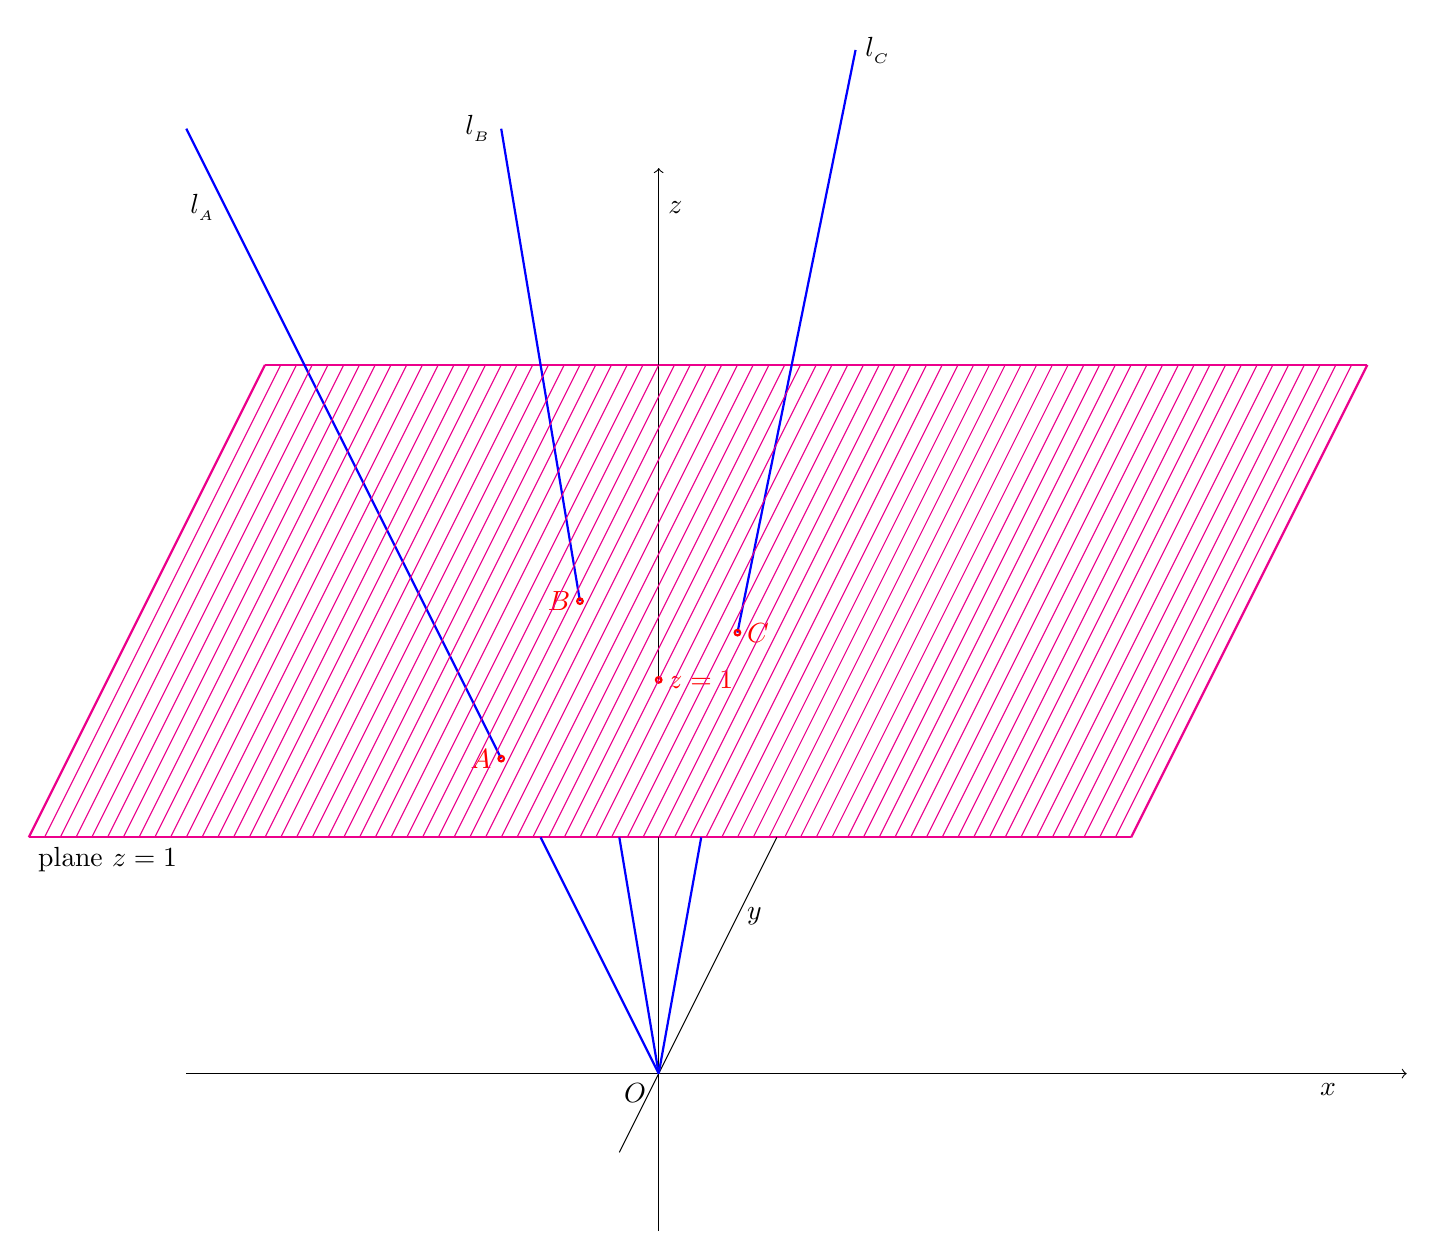
\begin{tikzpicture}
%\draw [help lines] (-10,-6) grid (6,6);

% plane $\pi$


\draw [   magenta, thick] (-10,-2)--(4,-2);
\draw [   magenta, thick] (-10,-2)--(-7,4);
\draw [   magenta, thick] (-7,4)--(7,4);
\draw [   magenta, thick] (4,-2)--(7,4);

  % origin at the point (-2,-5)
\node [below] at (-2.3,-5) {$O$};

  % Coordinate axis through the origin
\draw [ -> , thin] (-8,-5)--(7.5,-5);
\node [below] at (6.5,-5) {$x$};
\draw [  thin] (-2,-7)--(-2,-2);
%\draw [  thin,dashed ] (-2,-2)--(-2,0);
\draw [ -> , thin] (-2,0)--(-2,6.5);
\node [right] at (-2,6) {$z$};
\draw [ thin] (-2.5,-6)--(-0.5,-2);
\node [right] at (-1,-3) {$y$};



% point at $z=1$, this is the point (-2,0)
\draw [red, thick] (-2,0) circle (1pt);
\node [right,red] at (-2,0) {$z=1$};

% points $A,B,C$ at the plane

     % point A
\draw [blue, thick] (-2,-5)--(-3.5,-2);
\draw [blue, thick] (-4,-1)--(-8,7);
\node [left] at (-7.5,6) {$l_{_A}$};
\draw [red, thick] (-4,-1) circle (1pt);
\node [left,red] at (-4,-1) {$A$};
        % point B
\draw [blue, thick] (-2,-5)--(-2.5,-2);
\draw [blue, thick] (-3,1)--(-4,7);
\node [left] at (-4,7) {$l_{_B}$};
\draw [red, thick] (-3,1) circle (1pt);
\node [left,red] at (-3,1) {$B$};
      

        % point C
\draw [blue, thick] (-2,-5)--(-1.46,-2);
\draw [blue, thick] (-1,0.6)--(0.5,8);
\node [right] at (0.5,8) {$l_{_C}$};
\draw [red, thick] (-1,0.6) circle (1pt);
\node [right,red] at (-1,0.6) {$C$};



%  shtrikhovka:

\draw [   magenta, thin] (-9.8,-2)--(-6.8,4);
\draw [   magenta, thin] (-9.6,-2)--(-6.6,4);
\draw [   magenta, thin] (-9.4,-2)--(-6.4,4);
\draw [   magenta, thin] (-9.2,-2)--(-6.2,4);
\draw [   magenta, thin] (-9.0,-2)--(-6.0,4);
\draw [   magenta, thin] (-8.8,-2)--(-5.8,4);
\draw [   magenta, thin] (-8.6,-2)--(-5.6,4);
\draw [   magenta, thin] (-8.4,-2)--(-5.4,4);
\draw [   magenta, thin] (-8.2,-2)--(-5.2,4);
\draw [   magenta, thin] (-8.0,-2)--(-5.0,4);
\draw [   magenta, thin] (-7.8,-2)--(-4.8,4);
\draw [   magenta, thin] (-7.6,-2)--(-4.6,4);
\draw [   magenta, thin] (-7.4,-2)--(-4.4,4);
\draw [   magenta, thin] (-7.2,-2)--(-4.2,4);
\draw [   magenta, thin] (-7.0,-2)--(-4.0,4);
\draw [   magenta, thin] (-6.8,-2)--(-3.8,4);
\draw [   magenta, thin] (-6.6,-2)--(-3.6,4);
\draw [   magenta, thin] (-6.4,-2)--(-3.4,4);
\draw [   magenta, thin] (-6.2,-2)--(-3.2,4);
\draw [   magenta, thin] (-6.0,-2)--(-3.0,4);
\draw [   magenta, thin] (-5.8,-2)--(-2.8,4);
\draw [   magenta, thin] (-5.6,-2)--(-2.6,4);
\draw [   magenta, thin] (-5.4,-2)--(-2.4,4);
\draw [   magenta, thin] (-5.2,-2)--(-2.2,4);
\draw [   magenta, thin] (-5.0,-2)--(-2.0,4);
\draw [   magenta, thin] (-4.8,-2)--(-1.8,4);
\draw [   magenta, thin] (-4.6,-2)--(-1.6,4);
\draw [   magenta, thin] (-4.4,-2)--(-1.4,4);
\draw [   magenta, thin] (-4.2,-2)--(-1.2,4);
\draw [   magenta, thin] (-4.0,-2)--(-1.0,4);
\draw [   magenta, thin] (-3.8,-2)--(-0.8,4);
\draw [   magenta, thin] (-3.6,-2)--(-0.6,4);
\draw [   magenta, thin] (-3.4,-2)--(-0.4,4);
\draw [   magenta, thin] (-3.2,-2)--(-0.2,4);
\draw [   magenta, thin] (-3.0,-2)--(0.0,4);
\draw [   magenta, thin] (-2.8,-2)--(0.2,4);
\draw [   magenta, thin] (-2.6,-2)--(0.4,4);
\draw [   magenta, thin] (-2.4,-2)--(0.6,4);
\draw [   magenta, thin] (-2.2,-2)--(0.8,4);
\draw [   magenta, thin] (-2.0,-2)--(1.0 ,4);
\draw [   magenta, thin] (-1.8,-2)--(1.2,4);
\draw [   magenta, thin] (-1.6,-2)--(1.4,4);
\draw [   magenta, thin] (-1.4,-2)--(1.6,4);
\draw [   magenta, thin] (-1.2,-2)--(1.8,4);
\draw [   magenta, thin] (-1.0,-2)--(2,4);
\draw [   magenta, thin] (-0.8,-2)--(2.2,4);
\draw [   magenta, thin] (-0.6,-2)--(2.4,4);
\draw [   magenta, thin] (-0.4,-2)--(2.6,4);
\draw [   magenta, thin] (-0.2,-2)--(2.8,4);
\draw [   magenta, thin] (0.0,-2)--(3.0,4);
\draw [   magenta, thin] (0.2,-2)--(3.2,4);
\draw [   magenta, thin] (0.4,-2)--(3.4,4);
\draw [   magenta, thin] (0.6,-2)--(3.6,4);
\draw [   magenta, thin] (0.8,-2)--(3.8,4);
\draw [   magenta, thin] (1.0,-2)--(4,4);
\draw [   magenta, thin] (1.2,-2)--(4.2,4);
\draw [   magenta, thin] (1.4,-2)--(4.4,4);
\draw [   magenta, thin] (1.6,-2)--(4.6,4);
\draw [   magenta, thin] (1.8,-2)--(4.8,4);
\draw [   magenta, thin] (2.0,-2)--(5,4);
\draw [   magenta, thin] (2.2,-2)--(5.2,4);
\draw [   magenta, thin] (2.4,-2)--(5.4,4);
\draw [   magenta, thin] (2.6,-2)--(5.6,4);
\draw [   magenta, thin] (2.8,-2)--(5.8,4);
\draw [   magenta, thin] (3.0,-2)--(6.0,4);
\draw [   magenta, thin] (3.2,-2)--(6.2,4);
\draw [   magenta, thin] (3.4,-2)--(6.4,4);
\draw [   magenta, thin] (3.6,-2)--(6.6,4);
\draw [   magenta, thin] (3.8,-2)--(6.8,4);


\node [below] at (-9,-2) {${{\rm plane}\,\, z=1}$};


\end{tikzpicture}

\begin{equation*}
\hbox {plane}\,\, \pi\colon\quad z=1\,.
\end{equation*}
         \begin{equation*}
\R\P^2=\{l\colon \l\in\R^3\}
         \end{equation*}


        \centerline
     {
``A point'' in $\R\P^2$''  $=$ line in $\R^3$
  passing through  the origin
          }


\begin {equation*}
\begin{matrix}
\hbox{a point}\,\, A--- \hbox{line}\,\, l_{A}\cr
             \cr
\hbox{a point}\,\, B--- \hbox{line}\,\, l_{B}\cr
\cr
\hbox{a point}\,\, C--- \hbox{line}\,\, l_{C}\cr   
 \end{matrix}
\end {equation*}

However there are many `points' which are represented
by lines which are parallel to the plane $\pi$

    \begin {equation*}
\begin{matrix}
\hbox{a point $A$ on the plane $\pi$}--- \hbox{line $l_{A}$ 
                          which intersects this
             plane}\cr
             \cr
\hbox {a point at infinity}---   \hbox {line which is parallel to
                                       the plane $\pi$}\cr
 \end{matrix}
\end {equation*}

%\end{document}  % the last reading week 1 May 2018
 
    \subsubsection {Homogeneous and affine coordinates in $\R\P^2$}
Now we define homogeneous and affine coordinates of points
in projective plane, in the way similar as
we defined homogeneous and affine coordinates on projective line 
$\R\P$.

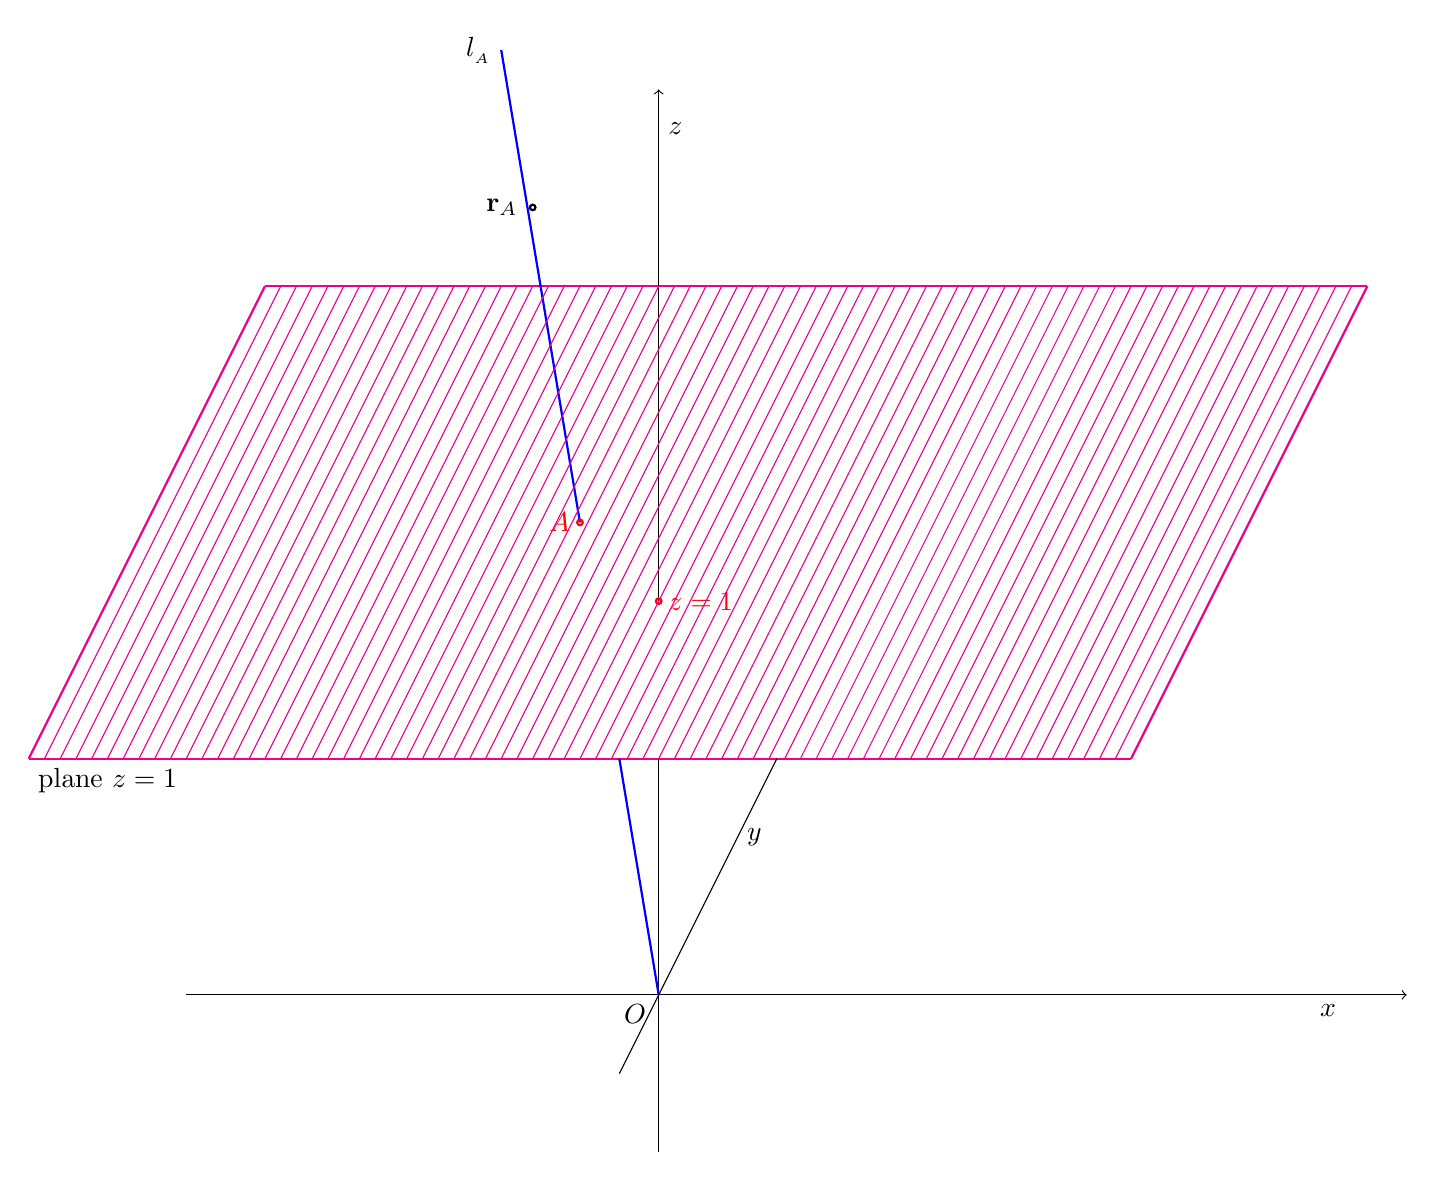
\begin{tikzpicture}
%\draw [help lines] (-10,-6) grid (6,6);

% plane $\pi$


\draw [   magenta, thick] (-10,-2)--(4,-2);
\draw [   magenta, thick] (-10,-2)--(-7,4);
\draw [   magenta, thick] (-7,4)--(7,4);
\draw [   magenta, thick] (4,-2)--(7,4);

  % origin at the point (-2,-5)
\node [below] at (-2.3,-5) {$O$};

  % Coordinate axis through the origin
\draw [ -> , thin] (-8,-5)--(7.5,-5);
\node [below] at (6.5,-5) {$x$};
\draw [  thin] (-2,-7)--(-2,-2);
%\draw [  thin,dashed ] (-2,-2)--(-2,0);
\draw [ -> , thin] (-2,0)--(-2,6.5);
\node [right] at (-2,6) {$z$};
\draw [ thin] (-2.5,-6)--(-0.5,-2);
\node [right] at (-1,-3) {$y$};



% point at $z=1$, this is the point (-2,0)
\draw [red, thick] (-2,0) circle (1pt);
\node [right,red] at (-2,0) {$z=1$};

% points $A,B,C$ at the plane

     % point A
%\draw [blue, thick] (-2,-5)--(-3.5,-2);
%\draw [blue, thick] (-4,-1)--(-8,7);
%\node [left] at (-7.5,6) {$l_{_A}$};
%\draw [red, thick] (-4,-1) circle (1pt);
%\node [left,red] at (-4,-1) {$A$};
        % point A
\draw [blue, thick] (-2,-5)--(-2.5,-2);
\draw [blue, thick] (-3,1)--(-4,7);
\node [left] at (-4,7) {$l_{_A}$};
\draw [ thick] (-3.6,5) circle (1pt);
\node [left] at (-3.67,5) {$\r_A$};
\draw [red, thick] (-3,1) circle (1pt);
\node [left,red] at (-3,1) {$A$};
      

        % point C
%\draw [blue, thick] (-2,-5)--(-1.46,-2);
%\draw [blue, thick] (-1,0.6)--(0.5,8);
%\node [right] at (0.5,8) {$l_{_C}$};
%\draw [red, thick] (-1,0.6) circle (1pt);
%\node [right,red] at (-1,0.6) {$C$};



%  shtrikhovka:

\draw [   magenta, thin] (-9.8,-2)--(-6.8,4);
\draw [   magenta, thin] (-9.6,-2)--(-6.6,4);
\draw [   magenta, thin] (-9.4,-2)--(-6.4,4);
\draw [   magenta, thin] (-9.2,-2)--(-6.2,4);
\draw [   magenta, thin] (-9.0,-2)--(-6.0,4);
\draw [   magenta, thin] (-8.8,-2)--(-5.8,4);
\draw [   magenta, thin] (-8.6,-2)--(-5.6,4);
\draw [   magenta, thin] (-8.4,-2)--(-5.4,4);
\draw [   magenta, thin] (-8.2,-2)--(-5.2,4);
\draw [   magenta, thin] (-8.0,-2)--(-5.0,4);
\draw [   magenta, thin] (-7.8,-2)--(-4.8,4);
\draw [   magenta, thin] (-7.6,-2)--(-4.6,4);
\draw [   magenta, thin] (-7.4,-2)--(-4.4,4);
\draw [   magenta, thin] (-7.2,-2)--(-4.2,4);
\draw [   magenta, thin] (-7.0,-2)--(-4.0,4);
\draw [   magenta, thin] (-6.8,-2)--(-3.8,4);
\draw [   magenta, thin] (-6.6,-2)--(-3.6,4);
\draw [   magenta, thin] (-6.4,-2)--(-3.4,4);
\draw [   magenta, thin] (-6.2,-2)--(-3.2,4);
\draw [   magenta, thin] (-6.0,-2)--(-3.0,4);
\draw [   magenta, thin] (-5.8,-2)--(-2.8,4);
\draw [   magenta, thin] (-5.6,-2)--(-2.6,4);
\draw [   magenta, thin] (-5.4,-2)--(-2.4,4);
\draw [   magenta, thin] (-5.2,-2)--(-2.2,4);
\draw [   magenta, thin] (-5.0,-2)--(-2.0,4);
\draw [   magenta, thin] (-4.8,-2)--(-1.8,4);
\draw [   magenta, thin] (-4.6,-2)--(-1.6,4);
\draw [   magenta, thin] (-4.4,-2)--(-1.4,4);
\draw [   magenta, thin] (-4.2,-2)--(-1.2,4);
\draw [   magenta, thin] (-4.0,-2)--(-1.0,4);
\draw [   magenta, thin] (-3.8,-2)--(-0.8,4);
\draw [   magenta, thin] (-3.6,-2)--(-0.6,4);
\draw [   magenta, thin] (-3.4,-2)--(-0.4,4);
\draw [   magenta, thin] (-3.2,-2)--(-0.2,4);
\draw [   magenta, thin] (-3.0,-2)--(0.0,4);
\draw [   magenta, thin] (-2.8,-2)--(0.2,4);
\draw [   magenta, thin] (-2.6,-2)--(0.4,4);
\draw [   magenta, thin] (-2.4,-2)--(0.6,4);
\draw [   magenta, thin] (-2.2,-2)--(0.8,4);
\draw [   magenta, thin] (-2.0,-2)--(1.0 ,4);
\draw [   magenta, thin] (-1.8,-2)--(1.2,4);
\draw [   magenta, thin] (-1.6,-2)--(1.4,4);
\draw [   magenta, thin] (-1.4,-2)--(1.6,4);
\draw [   magenta, thin] (-1.2,-2)--(1.8,4);
\draw [   magenta, thin] (-1.0,-2)--(2,4);
\draw [   magenta, thin] (-0.8,-2)--(2.2,4);
\draw [   magenta, thin] (-0.6,-2)--(2.4,4);
\draw [   magenta, thin] (-0.4,-2)--(2.6,4);
\draw [   magenta, thin] (-0.2,-2)--(2.8,4);
\draw [   magenta, thin] (0.0,-2)--(3.0,4);
\draw [   magenta, thin] (0.2,-2)--(3.2,4);
\draw [   magenta, thin] (0.4,-2)--(3.4,4);
\draw [   magenta, thin] (0.6,-2)--(3.6,4);
\draw [   magenta, thin] (0.8,-2)--(3.8,4);
\draw [   magenta, thin] (1.0,-2)--(4,4);
\draw [   magenta, thin] (1.2,-2)--(4.2,4);
\draw [   magenta, thin] (1.4,-2)--(4.4,4);
\draw [   magenta, thin] (1.6,-2)--(4.6,4);
\draw [   magenta, thin] (1.8,-2)--(4.8,4);
\draw [   magenta, thin] (2.0,-2)--(5,4);
\draw [   magenta, thin] (2.2,-2)--(5.2,4);
\draw [   magenta, thin] (2.4,-2)--(5.4,4);
\draw [   magenta, thin] (2.6,-2)--(5.6,4);
\draw [   magenta, thin] (2.8,-2)--(5.8,4);
\draw [   magenta, thin] (3.0,-2)--(6.0,4);
\draw [   magenta, thin] (3.2,-2)--(6.2,4);
\draw [   magenta, thin] (3.4,-2)--(6.4,4);
\draw [   magenta, thin] (3.6,-2)--(6.6,4);
\draw [   magenta, thin] (3.8,-2)--(6.8,4);


\node [below] at (-9,-2) {${{\rm plane}\,\, z=1}$};


\end{tikzpicture}


%\begin{table}\centering
%   \begin{tabular}{cc}
%\end{tabular}
%\end{table}
            
   \begin{equation*}
     \begin{matrix}
\hbox {A point $A=[x_A:y_A:z_A]$}\cr
\hbox { in $\R\P^2$}\cr
  ([x_A:y_A:z_A]=\cr
  =[\lambda x_A:\lambda y_A:\lambda z_A])\cr
          [x:y:z]-\cr
     \hbox{homogeneous }\cr
     \hbox {coordinates}\cr
    \hbox{of a point in $\R\P^2$}\cr
     \end{matrix}\quad
            \begin{matrix}
  \hbox {line $l$ which passes }\cr
    \hbox {through the origin}\cr
    \hbox {and a point $\r_A$}\cr
          l\colon \begin{cases}
                 x=tx_A\cr
                  y=ty_A\cr
                  z=tz_A\cr
                  \end{cases}
                          \cr
           \r_A=(x_A,y_A,z_A)\cr
               \r=t\r_A\cr
            -\infty<t<\infty\cr
             \end{matrix}
   \end{equation*}

\smallskip


{\bf Example}
       \begin{equation*}
     \begin{matrix}
\hbox {A point $A=[2:3:5]$}\cr
\hbox { in $\R\P^2$}\cr
  ([2:3:5]=\cr
  =[4:6:10]=[6:9:15)
          [x:y:z]-\cr
     \hbox{homogeneous }\cr
     \hbox {coordinates}\cr
    \hbox{of the point }\cr
    \hbox{ $A$ in $\R\P^2$}\cr
     \end{matrix}\quad
            \begin{matrix}
  \hbox {line $l$ which passes }\cr
    \hbox {through the origin}\cr
    \hbox {and a point $\r_A$}\cr
          l\colon \begin{cases}
                 x=2t\cr
                  y=6t\cr
                  z=5t\cr
                  \end{cases}
                          \cr
           \r_A=(2,3,5)\cr
               \r=t\r_A\cr
            -\infty<t<\infty\cr
             \end{matrix}
   \end{equation*}


 In the same way as for projective line {\it finite} points
are points which are represented by lines which intersect the plane
$\pi\colon z=1$, i.e. lines which do not belong to 
   the plane $OXY$.   The homogeneous coordinates of
finite points $[x:y:z]$ obey condition
        \begin{equation}\label{finitepoint}
            z\not=0\,.
           \end{equation}
Consider an arbitrary point  $A=[a:b:c]$,
such that this condition is obeyed, $c\not=0$.
Then we have that  for arbitrary $\lambda\not=0$
                 $$
       [a:b:c]=
           \left[
         {a\over \lambda}:
         {b\over \lambda}:
         {c\over \lambda}
                  \right]\Rightarrow
[a:b:c]=    \left[
         {a\over c}:
         {b\over c}:
                1
                  \right]\,.
                  $$
This relation says that these three points of $\R^3$,
   the point $(a,b,c)$, the point   
$\left(
         {a\over \lambda},
         {b\over \lambda},
         {c\over \lambda}
                  \right)$ and the point
 $\left(
         {a\over c},
         {b\over c},
                1
                  \right)$ 
belong  to the line
    $l_A$; this line  represents the `point' $A=[a:b:c]$ of the projective
plane $\R\P^2$. The point (usual point of $\R^3$)
 $\left(
         {a\over c},
         {b\over c},
                1
                  \right)$ 
belongs to the plane $\pi\colon\quad z=0$, and
    ${a\over c},{b\over c}$ are $x,y$-coordinates of the 
intersection of the line $l_A$ with the plane  $\pi$.

 
{\bf Definition} Let $A=[x:y:z]$ be an arbitrary finite point
of the projective plane $\R^2$, ($z\not=0$).
 {\it Affine coordinates} $u_A$ and $v_A$
of this point are:
       \begin{equation}\label{affinecoordinates}
             u_A={x\over z}\,,
             v_A={y\over z}\,.
           \end{equation}
      (Compare with affine coordinate for projective line (see
 \eqref{affinecoordinate}).)


  What about points at infinity, i.e. points $[x:y:z]$ such that $z=0$?
One can see that these `points' on the projective plane
are represented by lines in $\R^3$
   which belong to the plane $OXY$. These lines
pass through the origin and  are parallel to the plane $\pi$.



In the case of projective line $\R\P$ we had just one point
at infinity.   Now on projective plane $\R\P^2$ we 
have the infinite set of `points' at infinity
$=$ the set of lines in the plane $OXY$ passing through the origin.
On the other hand the set of lines in the plane $OXY$ passing through
the origin is nothing but projective line.
In its turn we know that projective line is a line completed
by a point at infinity. 


  We come to the following
 
\bigskip 
         
 \centerline   { {\LARGE  Matrjoshka}}
        \begin{equation}
        \R\P^2=\underbrace{\R^2}_
{\hbox{\footnotesize finite points on $\R\P^2$} }\cup 
        \underbrace{\R\P}_
{\hbox{\footnotesize points at infinity} } 
        \end{equation}

The projective line of points at infinity is $\R\P$:
              \begin{equation*}
          \begin{pmatrix}
        \hbox{points at infinity}\cr 
        \hbox{(invisible points)}\cr 
              \end{pmatrix}                   
                    \,=\,  
          \begin{pmatrix}
        \hbox{lines in OXY}\cr 
        \hbox{passing through the origin}\cr
          \end{pmatrix}
                \,=\, \R\P 
              \end{equation*}
We come to  

        \begin{equation}
      \R\P^2=  \R^2\cup\R\P=\R^2\cup\left(\R\cup {\infty}\right)\,.
        \end{equation}
{\footnotesize One can define $n$-dimensional projective space $\R\P^n$
as a space of lines in $\R^{n+1}$ passing through the origin. We come
to ``matrjoshka'' with $n$ 1dolls'. E.g.
                    $$
\R\P^3=
\R^3\cup \R\P^2=
\R^3\cup \left(\R^2\cup \R\P\right)=
\R^3\cup \left(\R^2\cup \left(\R\cup \{\infty\}\right)\right)\,.
                    $$
}
                 
      
 \subsubsection {Lines in $\R\P^2$ and 
collinear points in $\R\P^2$}

We know that the points on the projective plane $\R\P^2$ are 
the lines in $\R^3$
which pass through the origin.
What about `lines' on the projective plane $\R\P^2$? 

{\bf Definition}  `Lines' in projective plane $\R\P^2$
are the planes in $\R^3$ which pass through the origin. 

\smallskip



Pick two  points $A$ and $B$ on the projective plane $\R\P^2$.
Let these points be represented by lines $l_A,l_B$ in $\R^3$:
   \begin{equation*}
                  \begin{matrix}
 \hbox {Points $A,B$}\cr
 \hbox{in $\R\P^2$}\cr
                     \end{matrix}
               \,\, -\,\,
                   \begin{matrix}
 \hbox {lines $l_A,l_B$}\cr
 \hbox{in $\R^3$}\cr
                     \end{matrix}
               \end{equation*}

\m

Draw the `line' in $\R\P^2$ which passes through `points'  $A,B$
              \begin{equation*}
                  \begin{matrix}
 \hbox {Line $AB$ in $\R\P^2$}\cr
 \hbox{passing through `points' }\cr
 \hbox{ $A$ and $B$}\cr
                     \end{matrix}
                          \quad
                   \begin{matrix}
 \hbox {plane in $\R^3$}\cr
 \hbox{passing through lines}\cr
 \hbox{$l_A,l_B$}\cr
                     \end{matrix}
               \end{equation*}

The `points' of the `line' $AB$  in $\R\P^2$ are represented by 
lines in the plane $\a$  which pass  through origin.
(see Figure \eqref{lineintheprojectiveplane}.)

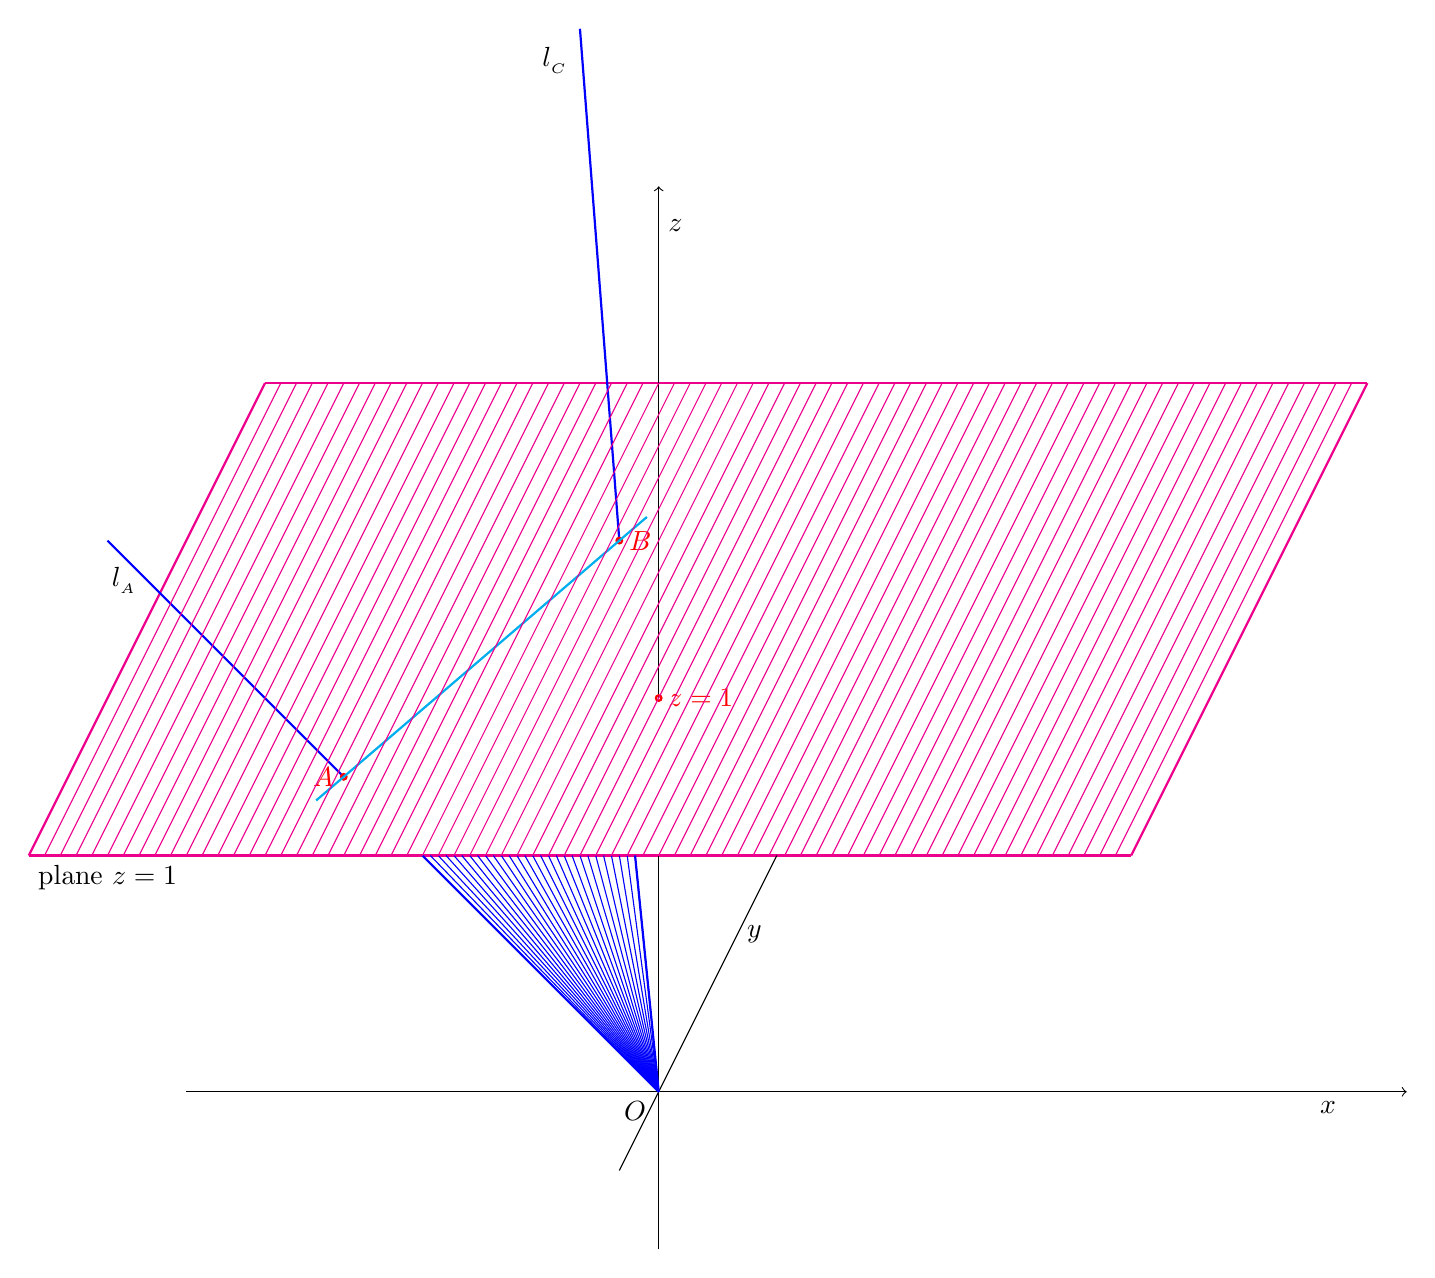
\begin{tikzpicture}
%\draw [help lines] (-10,-6) grid (6,6);

% plane $\pi$


\draw [   magenta, thick] (-10,-2)--(4,-2);
\draw [   magenta, thick] (-10,-2)--(-7,4);
\draw [   magenta, thick] (-7,4)--(7,4);
\draw [   magenta, thick] (4,-2)--(7,4);

  % origin at the point (-2,-5)
\node [below] at (-2.3,-5) {$O$};

  % Coordinate axis through the origin
\draw [ -> , thin] (-8,-5)--(7.5,-5);
\node [below] at (6.5,-5) {$x$};
\draw [  thin] (-2,-7)--(-2,-2);
%\draw [  thin,dashed ] (-2,-2)--(-2,0);
\draw [ -> , thin] (-2,0)--(-2,6.5);
\node [right] at (-2,6) {$z$};
\draw [ thin] (-2.5,-6)--(-0.5,-2);
\node [right] at (-1,-3) {$y$};



% point at $z=1$, this is the point (-2,0)
\draw [red, thick] (-2,0) circle (1pt);
\node [right,red] at (-2,0) {$z=1$};

% points $A,B,C$ at the plane

     % point A
\draw [blue, thick] (-2,-5)--(-5,-2);
\draw [blue, thick] (-6,-1)--(-9,2);
\node [left] at (-8.5,1.5) {$l_{_A}$};
\draw [red, thick] (-6,-1) circle (1pt);
\node [left,red] at (-6,-1) {$A$};

        % point B
%\draw [blue, thick] (-2,-5)--(-2.5,-2);
%\draw [blue, thick] (-3,1)--(-4,7);
%\node [left] at (-4,7) {$l_{_B}$};
%\draw [red, thick] (-3,1) circle (1pt);
%\node [left,red] at (-3,1) {$B$};
      

        % point C
\draw [blue, thick] (-2,-5)--(-2.3,-2);
\draw [blue, thick] (-2.5,2)--(-3,8.5);
\node [right] at (-3.6,8.1) {$l_{_C}$};
\draw [red, thick] (-2.5,2) circle (1pt);
\node [right,red] at (-2.5,2) {$B$};

% these points are at the same line:  ABC



\draw [thick, cyan] (-6.35, -1.3)--(-2.15,2.3);

% plane $\a$ which passes through points $A,B,0)$
% vmeste s shtrikhovkoj

\draw [thin, blue] (-2,-5)--(-4.9,-2);
\draw [thin, blue] (-2,-5)--(-4.8,-2);
\draw [thin, blue] (-2,-5)--(-4.7,-2);
\draw [thin, blue] (-2,-5)--(-4.6,-2);
\draw [thin, blue] (-2,-5)--(-4.5,-2);
\draw [thin, blue] (-2,-5)--(-4.4,-2);
\draw [thin, blue] (-2,-5)--(-4.3,-2);
\draw [thin, blue] (-2,-5)--(-4.2,-2);
\draw [thin, blue] (-2,-5)--(-4.1,-2);
\draw [thin, blue] (-2,-5)--(-4.0,-2);
\draw [thin, blue] (-2,-5)--(-3.9,-2);
\draw [thin, blue] (-2,-5)--(-3.8,-2);
\draw [thin, blue] (-2,-5)--(-3.7,-2);
\draw [thin, blue] (-2,-5)--(-3.6,-2);
\draw [thin, blue] (-2,-5)--(-3.5,-2);
\draw [thin, blue] (-2,-5)--(-3.4,-2);
\draw [thin, blue] (-2,-5)--(-3.3,-2);
\draw [thin, blue] (-2,-5)--(-3.2,-2);
\draw [thin, blue] (-2,-5)--(-3.1,-2);
\draw [thin, blue] (-2,-5)--(-3.0,-2);
\draw [thin, blue] (-2,-5)--(-2.9,-2);
\draw [thin, blue] (-2,-5)--(-2.8,-2);
\draw [thin, blue] (-2,-5)--(-2.7,-2);
\draw [thin, blue] (-2,-5)--(-2.6,-2);
\draw [thin, blue] (-2,-5)--(-2.5,-2);
\draw [thin, blue] (-2,-5)--(-2.4,-2);
\draw [thin, blue] (-2,-5)--(-2.3,-2);

%  shtrikhovka:

\draw [   magenta, thin] (-9.8,-2)--(-6.8,4);
\draw [   magenta, thin] (-9.6,-2)--(-6.6,4);
\draw [   magenta, thin] (-9.4,-2)--(-6.4,4);
\draw [   magenta, thin] (-9.2,-2)--(-6.2,4);
\draw [   magenta, thin] (-9.0,-2)--(-6.0,4);
\draw [   magenta, thin] (-8.8,-2)--(-5.8,4);
\draw [   magenta, thin] (-8.6,-2)--(-5.6,4);
\draw [   magenta, thin] (-8.4,-2)--(-5.4,4);
\draw [   magenta, thin] (-8.2,-2)--(-5.2,4);
\draw [   magenta, thin] (-8.0,-2)--(-5.0,4);
\draw [   magenta, thin] (-7.8,-2)--(-4.8,4);
\draw [   magenta, thin] (-7.6,-2)--(-4.6,4);
\draw [   magenta, thin] (-7.4,-2)--(-4.4,4);
\draw [   magenta, thin] (-7.2,-2)--(-4.2,4);
\draw [   magenta, thin] (-7.0,-2)--(-4.0,4);
\draw [   magenta, thin] (-6.8,-2)--(-3.8,4);
\draw [   magenta, thin] (-6.6,-2)--(-3.6,4);
\draw [   magenta, thin] (-6.4,-2)--(-3.4,4);
\draw [   magenta, thin] (-6.2,-2)--(-3.2,4);
\draw [   magenta, thin] (-6.0,-2)--(-3.0,4);
\draw [   magenta, thin] (-5.8,-2)--(-2.8,4);
\draw [   magenta, thin] (-5.6,-2)--(-2.6,4);
\draw [   magenta, thin] (-5.4,-2)--(-2.4,4);
\draw [   magenta, thin] (-5.2,-2)--(-2.2,4);
\draw [   magenta, thin] (-5.0,-2)--(-2.0,4);
\draw [   magenta, thin] (-4.8,-2)--(-1.8,4);
\draw [   magenta, thin] (-4.6,-2)--(-1.6,4);
\draw [   magenta, thin] (-4.4,-2)--(-1.4,4);
\draw [   magenta, thin] (-4.2,-2)--(-1.2,4);
\draw [   magenta, thin] (-4.0,-2)--(-1.0,4);
\draw [   magenta, thin] (-3.8,-2)--(-0.8,4);
\draw [   magenta, thin] (-3.6,-2)--(-0.6,4);
\draw [   magenta, thin] (-3.4,-2)--(-0.4,4);
\draw [   magenta, thin] (-3.2,-2)--(-0.2,4);
\draw [   magenta, thin] (-3.0,-2)--(0.0,4);
\draw [   magenta, thin] (-2.8,-2)--(0.2,4);
\draw [   magenta, thin] (-2.6,-2)--(0.4,4);
\draw [   magenta, thin] (-2.4,-2)--(0.6,4);
\draw [   magenta, thin] (-2.2,-2)--(0.8,4);
\draw [   magenta, thin] (-2.0,-2)--(1.0 ,4);
\draw [   magenta, thin] (-1.8,-2)--(1.2,4);
\draw [   magenta, thin] (-1.6,-2)--(1.4,4);
\draw [   magenta, thin] (-1.4,-2)--(1.6,4);
\draw [   magenta, thin] (-1.2,-2)--(1.8,4);
\draw [   magenta, thin] (-1.0,-2)--(2,4);
\draw [   magenta, thin] (-0.8,-2)--(2.2,4);
\draw [   magenta, thin] (-0.6,-2)--(2.4,4);
\draw [   magenta, thin] (-0.4,-2)--(2.6,4);
\draw [   magenta, thin] (-0.2,-2)--(2.8,4);
\draw [   magenta, thin] (0.0,-2)--(3.0,4);
\draw [   magenta, thin] (0.2,-2)--(3.2,4);
\draw [   magenta, thin] (0.4,-2)--(3.4,4);
\draw [   magenta, thin] (0.6,-2)--(3.6,4);
\draw [   magenta, thin] (0.8,-2)--(3.8,4);
\draw [   magenta, thin] (1.0,-2)--(4,4);
\draw [   magenta, thin] (1.2,-2)--(4.2,4);
\draw [   magenta, thin] (1.4,-2)--(4.4,4);
\draw [   magenta, thin] (1.6,-2)--(4.6,4);
\draw [   magenta, thin] (1.8,-2)--(4.8,4);
\draw [   magenta, thin] (2.0,-2)--(5,4);
\draw [   magenta, thin] (2.2,-2)--(5.2,4);
\draw [   magenta, thin] (2.4,-2)--(5.4,4);
\draw [   magenta, thin] (2.6,-2)--(5.6,4);
\draw [   magenta, thin] (2.8,-2)--(5.8,4);
\draw [   magenta, thin] (3.0,-2)--(6.0,4);
\draw [   magenta, thin] (3.2,-2)--(6.2,4);
\draw [   magenta, thin] (3.4,-2)--(6.4,4);
\draw [   magenta, thin] (3.6,-2)--(6.6,4);
\draw [   magenta, thin] (3.8,-2)--(6.8,4);


\node [below] at (-9,-2) {${{\rm plane}\,\, z=1}$};


\end{tikzpicture}

\begin{equation}\label{lineintheprojectiveplane}
\end{equation}

\m

{\bf Definition} We say that three points $A,B$
and $C$ on the projective plane $\R\P^2$ are {\it collinear}
if these points belong to the same line, 
or in other words if a point $C$ belongs to the
line passsing through the points $A$ and $B$, $C\in (AB)$.

\smallskip

Derive the condition of collinearity of three  points.



%\end{document}  %2 May 2018


\begin{equation}\label{collinearpoints}
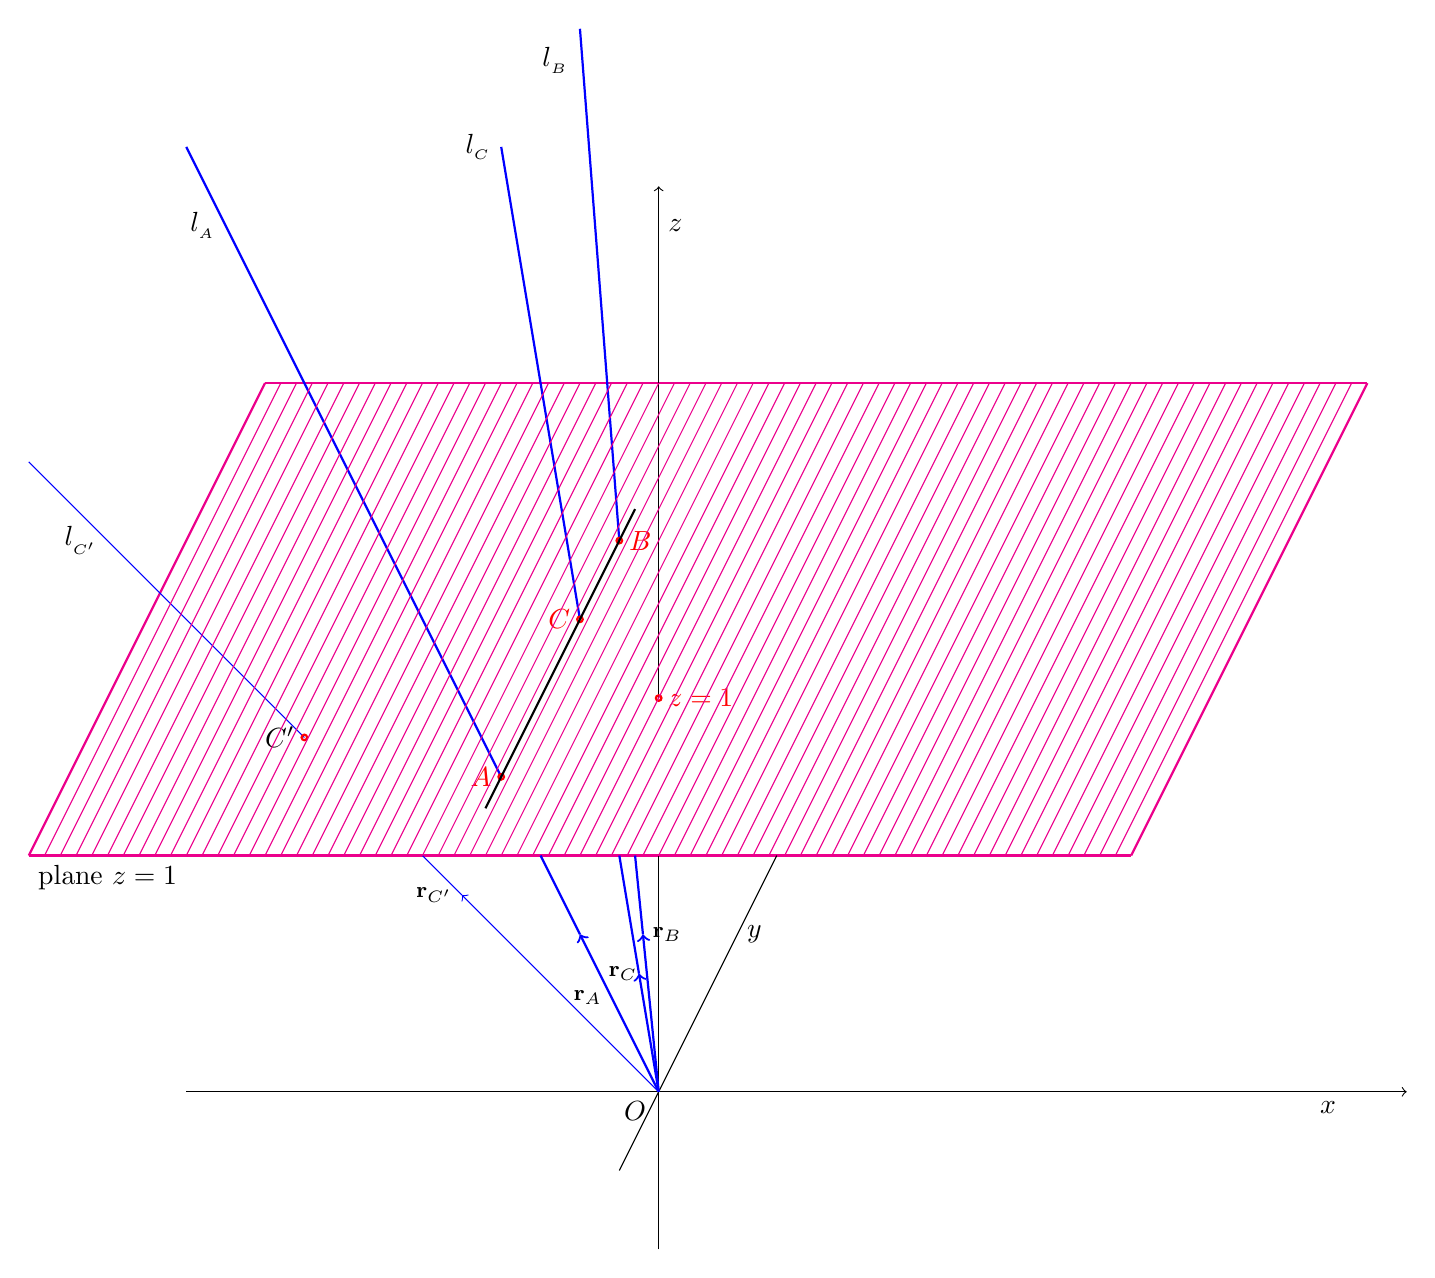
\begin{tikzpicture}
%\draw [help lines] (-10,-6) grid (6,6);

% plane $\pi$


\draw [   magenta, thick] (-10,-2)--(4,-2);
\draw [   magenta, thick] (-10,-2)--(-7,4);
\draw [   magenta, thick] (-7,4)--(7,4);
\draw [   magenta, thick] (4,-2)--(7,4);

  % origin at the point (-2,-5)
\node [below] at (-2.3,-5) {$O$};

  % Coordinate axis through the origin
\draw [ -> , thin] (-8,-5)--(7.5,-5);
\node [below] at (6.5,-5) {$x$};
\draw [  thin] (-2,-7)--(-2,-2);
%\draw [  thin,dashed ] (-2,-2)--(-2,0);
\draw [ -> , thin] (-2,0)--(-2,6.5);
\node [right] at (-2,6) {$z$};
\draw [ thin] (-2.5,-6)--(-0.5,-2);
\node [right] at (-1,-3) {$y$};



% point at $z=1$, this is the point (-2,0)
\draw [red, thick] (-2,0) circle (1pt);
\node [right,red] at (-2,0) {$z=1$};

% points $A,B,C$ at the plane

     % point A
\draw [blue, thick,->] (-2,-5)--(-3,-3);
\node [left] at (-2.6,-3.8) {$\hbox{\footnotesize $\r_A$}$};

\draw [blue, thick] (-3,-3)--(-3.5,-2);

\draw [blue, thick] (-4,-1)--(-8,7);
\node [left] at (-7.5,6) {$l_{_A}$};
\draw [red, thick] (-4,-1) circle (1pt);
\node [left,red] at (-4,-1) {$A$};


        % point C
\draw [blue, thick,->] (-2,-5)--(-2.25,-3.5);
\node [left] at (-2.15,-3.5) {$\hbox{\footnotesize $\r_C$}$};

\draw [blue, thick] (-2.25,-3.5)--(-2.5,-2);
\draw [blue, thick] (-3,1)--(-4,7);
\node [left] at (-4,7) {$l_{_C}$};
\draw [red, thick] (-3,1) circle (1pt);
\node [left,red] at (-3,1) {$C$};
      
        % point C' which is not on the same line
\draw [blue, thin,->] (-2,-5)--(-4.5,-2.5);
\node [left] at (-4.5,-2.5) {$\hbox{\footnotesize $\r_{C'}$}$};

\draw [blue, thin] (-4.5,-2.5)--(-5,-2);
\draw [blue, thin] (-6.5,-0.5)--(-10,3);
\node [left] at (-9,2) {$l_{_{C'}}$};
\draw [red, thick] (-6.5,-0.5) circle (1pt);
\node [left] at (-6.5,-0.5) {$C'$};
 
        % point B
\draw [blue, thick,->] (-2,-5)--(-2.2,-3);
\node [right] at (-2.2,-3) {$\hbox{\footnotesize $\r_B$}$};

\draw [blue, thick] (-2.2,-3)--(-2.3,-2);

\draw [blue, thick] (-2.5,2)--(-3,8.5);
\node [right] at (-3.6,8.1) {$l_{_B}$};
\draw [red, thick] (-2.5,2) circle (1pt);
\node [right,red] at (-2.5,2) {$B$};

% these points are at the same line:  ABC

\draw [thick] (-4.2, -1.4)--(-2.3,2.4);

%  shtrikhovka:

\draw [   magenta, thin] (-9.8,-2)--(-6.8,4);
\draw [   magenta, thin] (-9.6,-2)--(-6.6,4);
\draw [   magenta, thin] (-9.4,-2)--(-6.4,4);
\draw [   magenta, thin] (-9.2,-2)--(-6.2,4);
\draw [   magenta, thin] (-9.0,-2)--(-6.0,4);
\draw [   magenta, thin] (-8.8,-2)--(-5.8,4);
\draw [   magenta, thin] (-8.6,-2)--(-5.6,4);
\draw [   magenta, thin] (-8.4,-2)--(-5.4,4);
\draw [   magenta, thin] (-8.2,-2)--(-5.2,4);
\draw [   magenta, thin] (-8.0,-2)--(-5.0,4);
\draw [   magenta, thin] (-7.8,-2)--(-4.8,4);
\draw [   magenta, thin] (-7.6,-2)--(-4.6,4);
\draw [   magenta, thin] (-7.4,-2)--(-4.4,4);
\draw [   magenta, thin] (-7.2,-2)--(-4.2,4);
\draw [   magenta, thin] (-7.0,-2)--(-4.0,4);
\draw [   magenta, thin] (-6.8,-2)--(-3.8,4);
\draw [   magenta, thin] (-6.6,-2)--(-3.6,4);
\draw [   magenta, thin] (-6.4,-2)--(-3.4,4);
\draw [   magenta, thin] (-6.2,-2)--(-3.2,4);
\draw [   magenta, thin] (-6.0,-2)--(-3.0,4);
\draw [   magenta, thin] (-5.8,-2)--(-2.8,4);
\draw [   magenta, thin] (-5.6,-2)--(-2.6,4);
\draw [   magenta, thin] (-5.4,-2)--(-2.4,4);
\draw [   magenta, thin] (-5.2,-2)--(-2.2,4);
\draw [   magenta, thin] (-5.0,-2)--(-2.0,4);
\draw [   magenta, thin] (-4.8,-2)--(-1.8,4);
\draw [   magenta, thin] (-4.6,-2)--(-1.6,4);
\draw [   magenta, thin] (-4.4,-2)--(-1.4,4);
\draw [   magenta, thin] (-4.2,-2)--(-1.2,4);
\draw [   magenta, thin] (-4.0,-2)--(-1.0,4);
\draw [   magenta, thin] (-3.8,-2)--(-0.8,4);
\draw [   magenta, thin] (-3.6,-2)--(-0.6,4);
\draw [   magenta, thin] (-3.4,-2)--(-0.4,4);
\draw [   magenta, thin] (-3.2,-2)--(-0.2,4);
\draw [   magenta, thin] (-3.0,-2)--(0.0,4);
\draw [   magenta, thin] (-2.8,-2)--(0.2,4);
\draw [   magenta, thin] (-2.6,-2)--(0.4,4);
\draw [   magenta, thin] (-2.4,-2)--(0.6,4);
\draw [   magenta, thin] (-2.2,-2)--(0.8,4);
\draw [   magenta, thin] (-2.0,-2)--(1.0 ,4);
\draw [   magenta, thin] (-1.8,-2)--(1.2,4);
\draw [   magenta, thin] (-1.6,-2)--(1.4,4);
\draw [   magenta, thin] (-1.4,-2)--(1.6,4);
\draw [   magenta, thin] (-1.2,-2)--(1.8,4);
\draw [   magenta, thin] (-1.0,-2)--(2,4);
\draw [   magenta, thin] (-0.8,-2)--(2.2,4);
\draw [   magenta, thin] (-0.6,-2)--(2.4,4);
\draw [   magenta, thin] (-0.4,-2)--(2.6,4);
\draw [   magenta, thin] (-0.2,-2)--(2.8,4);
\draw [   magenta, thin] (0.0,-2)--(3.0,4);
\draw [   magenta, thin] (0.2,-2)--(3.2,4);
\draw [   magenta, thin] (0.4,-2)--(3.4,4);
\draw [   magenta, thin] (0.6,-2)--(3.6,4);
\draw [   magenta, thin] (0.8,-2)--(3.8,4);
\draw [   magenta, thin] (1.0,-2)--(4,4);
\draw [   magenta, thin] (1.2,-2)--(4.2,4);
\draw [   magenta, thin] (1.4,-2)--(4.4,4);
\draw [   magenta, thin] (1.6,-2)--(4.6,4);
\draw [   magenta, thin] (1.8,-2)--(4.8,4);
\draw [   magenta, thin] (2.0,-2)--(5,4);
\draw [   magenta, thin] (2.2,-2)--(5.2,4);
\draw [   magenta, thin] (2.4,-2)--(5.4,4);
\draw [   magenta, thin] (2.6,-2)--(5.6,4);
\draw [   magenta, thin] (2.8,-2)--(5.8,4);
\draw [   magenta, thin] (3.0,-2)--(6.0,4);
\draw [   magenta, thin] (3.2,-2)--(6.2,4);
\draw [   magenta, thin] (3.4,-2)--(6.4,4);
\draw [   magenta, thin] (3.6,-2)--(6.6,4);
\draw [   magenta, thin] (3.8,-2)--(6.8,4);


\node [below] at (-9,-2) {${{\rm plane}\,\, z=1}$};


\end{tikzpicture}
\hbox {Points $A,C,B$ are collinear}\,,\quad
\hbox {Points $A,C',B$ are not collinear}\,.
\end{equation}

As usual in the left column we will  write the statement about points
and lines in $\R\P^2$ and in the right column the representation
of these objects in $\R^3$.


             \begin{equation*}
            \begin{matrix}
   \hbox {points in $\R\P^2$}   & \hbox {lines in 
                    $\R^3$ }\cr
                          & \hbox {passing through the origin} \cr
                      \cr 
      A\in \R\P^2           & 0\in l_{A}\in \R^3\cr
  [x_A:y_A:z_A]            & \begin{cases} x=tx_A\cr y=ty_A\cr
                                        z=tz_A\end{cases}\,,\,\,
                              \r=t\r_A
                                       \cr             
       B\in \R\P^2           & 0\in l_{B}\in \R^3\cr
  [x_B:y_B:z_B]            & \begin{cases} x=tx_B\cr y=ty_B\cr
                                        z=tz_B\end{cases}\,,\,\,
                               \r=t\r_B
                             \cr             
        C\in \R\P^2           & 0\in l_{C}\in \R^3\cr
  [x_C:y_C:z_C]            & \begin{cases} x=tx_C\cr y=ty_C\cr
                                        z=tz_C\end{cases}\,,\,\,
                                  \r=t\r_C
                             \cr             
            \end{matrix}
              \end{equation*}
A parameter $t$ in these equations runs from $-\infty$ to $\infty$.

The vectors  
$\r_A=(x_A,y_A,z_A)$, 
$\r_B=(x_B,y_B,z_B)$ 
and $\r_C=(x_C,y_C,z_C)$ 
which span  respectively the lines $l_A$, $l_B$
and $l_C$
are  defined up to a non-zero multiplier (e.g. the vector $\r_A$ 
and the vector $3\r_A$ span the same line $l_A$). 


We see that point $C$ belongs to the line $AB$ if and only if
vectors 
$\r_A,\r_B$, $\r_C$ are linearly dependant, i.e.
         \begin{equation*}
  \gamma\r_A+\mu\r_B+\nu \r_C=0 \,,\,{\rm where}\, 
\lambda\not=0\,,{\rm or}\,
\mu\not=0\,,{\rm or}\,
\nu\not=0\,.
    \end{equation*}
i.e.
       \begin{equation}\label{criterion0ofcollinearity}
              \gamma 
         \begin{pmatrix}
      x_A\cr y_A\cr z_A
         \end{pmatrix}
                 +
                  \mu 
         \begin{pmatrix}
      x_B\cr y_B\cr z_B
         \end{pmatrix}
               +
   \nu 
         \begin{pmatrix}
      x_C\cr y_C\cr z_C
         \end{pmatrix}
            =0\,,\,
{\rm where}\, 
\lambda\not=0\,,{\rm or}\,
\mu\not=0\,,{\rm or}\,
\nu\not=0\,.
         \end{equation}
For example consider points $A,B$ and $C$ which are on the same line
in $\R\P^2$ (see Figure \eqref{collinearpoints}).
In this case vector $\r_C$ is the linear combination of vectors
$\r_A$ and $\r_B$. This means that these three vectors,
vectors $\r_A,\r_B, \r_C$ span the plane
in $\R^3$ passing through the origin. --- This is  equivalent to the fact
that three `points' $A,B,C$ on the projective plane
are on the one line (are collinear).

On the other consider the point  $C'$
in $\R\P^2$ (see Figure \eqref{collinearpoints}).
In this case vector $\r_{C'}$ is 
linearly independent on the vectors $\r_A$ and $\r_B$.
In this case  three vectors,
vectors $\r_A,\r_B, \r_C$ do not span the plane
in $\R^3$ (they span all $\R^3$!).---
This is equivalent to the fact  
that three `points' $A,B,C'$ on the projective plane
are not collinear.



  Recall that for arbitrary three vectors in $\R^3$  
one can consider the matrix such that components of these vectors
are columns (or rows) of this matrix. E.g. for vectors
   $\r_A=(x_A,y_A,z_A)$,
   $\r_B=(x_B,y_A,z_A)$,
   $\r_C=(x_C,y_C,z_C)$,
one can consider the matrix
   $$
   T_{ABC}=\begin{pmatrix}
             x_A & x_B & x_C\cr 
             y_A & y_B & y_C\cr 
             z_A & z_B & z_C\cr 
           \end{pmatrix},
   $$
and these vectors are linearly dependent if and only if the matrix
is degenerate $\Leftrightarrow$ non-invertible $\Leftrightarrow$ 
$\det T_{ABC}\not=0$.
Thus 
  condition \eqref{criterion0ofcollinearity} implies  

{\bf Proposition}\label{collinearity1}

{Let $A,B,C$ three points on the projective line
with homogeneous coordinates
  $A=[x_A:y_A:z_A]$,

  $B=[x_B:y_B:z_B]$,

  $C=[x_C:y_C:z_C]$.
These three points are collinear (belong to the same line)
if and only if the matrix
         \begin{equation}\label{collinearityeq1}
        T_{ABC}=\begin{pmatrix}
             x_A & x_B & x_C\cr 
             y_A & y_B & y_C\cr 
             z_A & z_B & z_C\cr 
           \end{pmatrix}
         \end{equation}
is degenerate $\Leftrightarrow$ $\det  T_{ABC}=0$\,.
}

{\bf Remark} We know that every  point in projective plane
may have different
homogeneous coordiantes:
        $$
[x:y:z]=[a x:ay:az]\,, (a\not=0)\,.
        $$
Changing homogeneous coordinates
of points do not change condition of degeneracy of matrix.
This is in accordance with the fact that   
condition of degeneracy of matrix $T_{ABC}$
($\det T_{ABC}=0$)
does not change if we multiply 
columns on arbitrary non-zero numbers:
vectors $\r_A,\r_B, \r_C$
are linearly dependant if and only if
vectors $a\r_A,\b\r_B,c\r_C$ are linearly dependant
  ($a,b,c\not=0$).  
   
  Suppose now points $A,B,C$ are finite points, i.e.
$z_A\not=0, z_B\not=0$ and $z_C\not=0$.
In this case one can consider not only homogeneous coordinates
 but also affine coordinates (see equation
\eqref{affinecoordinates}) of these points
          \begin{equation}\label{affinecoordinatesofthreepoints}
       \begin{matrix}
   A=[x_A:y_A:z_A]-& \hbox{affine coord.}\,\, 
                   u_A={x_A\over \z_A}\,, v_A={y_A\over\z_A}\cr
       \cr
          B=[x_B:y_B:z_B]-& \hbox{affine coord.}\,\, 
                   u_B={x_B\over \z_B}\,, v_B={y_B\over\z_B}\cr
       \cr
 C=[x_C:y_C:z_C]-& \hbox{affine coord.}\,\, 
                   u_C={x_C\over \z_C}\,, v_A={y_C\over\z_C}\cr
       \cr
\end{matrix}
      \end{equation} 
Proposition above states that
     $$
\hbox {points $A,B,C$ are collinear}\Leftrightarrow
  T_{ABC}\,\,\hbox {is degenerate matrix}\,.
     $$
Condition of degeneracy is not changed under the
multiplication of columns on non-zero numbers:
Multiplying 
the first column on $1\over z_A$,
the second column on $1\over z_B$, and
the third  column on $1\over z_C$ we come to 
     \begin{equation*}
 T_{ABC}\,\,\hbox {is degenerate }\,.
  \Leftrightarrow
  \hbox{the matrix }\,\, 
            \begin{pmatrix}
             {x_A\over z_A} & {x_B\over z_B} & {x_C\over z_C}\cr 
             {y_A\over z_A} & {y_B\over z_B} & {z_C\over z_C}\cr 
                    1 & 1  &  1\cr 
           \end{pmatrix}
        \,\, \hbox {is degenerate}.
\end{equation*}
Thus using \eqref{affinecoordinatesofthreepoints} we come to
the following fact:
          \begin{equation*}
\hbox{{\footnotesize finite points $A,B,C$ are collinear}}\Leftrightarrow
      \hbox {matrix}  \begin{pmatrix}
             u_A & u_B & u_C\cr 
             v_A & v_B & v_C\cr 
                    1 & 1  &  1\cr 
           \end{pmatrix}
    \,\, \hbox {{\footnotesize is degenerate}}.
   \end{equation*}
The condition of degeneracy of matrix 
in the right hand side of this equation means that 
its rows are linearly dependant\footnote{degeneracy 
$\Leftrightarrow$ colummns are linearly dependant 
$\Leftrightarrow$  rows are linearly dependant}, 
i.e.  there exist three numbers $p,q,r$
such that not all these numbers are equal to zero, and
         $$
pu_A+qv_A+r=
pu_B+qv_B+r=
pu_C+qv_C+r=0\,.
         $$
This means that these three points
are on the one line:
    \begin{equation}\label{collinearityaffine}
pu+qv+r=0\,.
    \end{equation}

We see that for finite points condition of collinearity
 becomes almost tautological.
  Of course we can check the collinearity of finite points,
finiding the line \eqref{collinearityaffine} 
such all these points belong to this line, or
we can use just Proposition \ref{collinearity1}.

Consider example

\m

{\bf Example} Consider three points

   $A=[1:-1:1]$, 
   
     $B=[10:-15:5]$,
 
   $C=\left[1:-{9\over 5}:{1\over 5}\right]$.

  Check are these points collinear or no.

   
Since these points are finite then the condition of collinearity
may be checked or using Proposition\ref{collinearity1}
or using criterion that they all belong to the same line
(see equation \eqref{collinearityaffine}).
 
   
\smallskip

{\tt First way: using Proposition}. Consider  the matrix 
$T_{ABC}=\begin{pmatrix}
      1 & 10 & 1\cr
      -1 & -15 & -{9\over 5}\cr
      1 & 5 & {1\over 5}\cr
   \end{pmatrix}$
One can see straightforwardly that this matrix is degenerate.
To facilitate considerations we may perform column operations,
and  multiply columns on suitable non-zero numbers:
mulitply second column on ${1\over 5}$,
and third on $5$
\footnote
{sure degeneracy condition
 does not depend on the choice of these numbers, ``suitable''
means to make calculations easier}.
We come to the matrix
 $T'_{ABC}=\begin{pmatrix}
      1 & 2 & 5\cr
      -1 & -3 & -9\cr
      1 & 1 & 1\cr
   \end{pmatrix}$.



The matrix  $T'_{ABC}$  is obviously degenerate matrix, since its determinant
vanishes.
  (It is much easier to see its degeneracy that the degeneracy of the
  matrix $T_{ABC}$.)

\m

{\tt II-nd  way: using affine coordinates}.
  Consider affine coordinates of the points $A,B,C$: 

     $u_A={x_A\over y_A}=1$, $v_A={y_A\over z_A}=-1$,
     
        $u_B={x_B\over y_B}=2$, $v_B={y_B\over z_B}=-3$,
     
     $u_C={x_C\over y_C}=5$, $v_C={y_C\over z_C}=-9$,
 
We see that
              \begin{equation}\label{exercisethreepointsontheline}
\begin{pmatrix}
       u_A\cr  v_A\cr
\end{pmatrix}
   =
\begin{pmatrix}
       1\cr -1\cr
\end{pmatrix}
 \,,\quad
 \begin{pmatrix}
       u_B\cr  v_B\cr
\end{pmatrix}
   =
\begin{pmatrix}
       2\cr -3\cr
\end{pmatrix}
 \,,\quad
 \begin{pmatrix}
       u_C\cr  v_C\cr
\end{pmatrix}
   =
\begin{pmatrix}
       5\cr -9\cr
\end{pmatrix}
 \,.
              \end{equation}
 All these points belong  to the one line
         $$
    2u+v=1\,.
         $$

Of course the second way is much shorter, but sometimes
it is not easy to guess an equation of the line \eqref{collinearityaffine}.

(See other examples in Homework 9)
 

\subsubsection {Cross-ratio of four 
collinear points in $\R\P^2$}

We know that for four points on projective line their cross-ratio
\eqref{crossratioaffine} is invariant of projective transfromations:
               \begin{equation}\label{crossratiohere}
   (A,B,C,D)={(u_A-u_C)(u_B-u_D)\over (u_A-u_D)(u_B-u_C)}
               \end{equation}
is an invariant of projective transformations:
If  $u'= {\a u+\beta\over \gamma u+\delta}$
is an arbitrary projective transformation
($\a\delta-\beta\gamma\not=0$) (see \eqref{projtransofline})
then
             $$
(A,B,C,D)={(u_A-u_C)(u_B-u_D)\over (u_A-u_D)(u_B-u_C)}=
             $$
          \begin{equation}\label{invarianceagain}
=(A',B',C',D')={(u_{A'}-u_{C'})(u_{B'}-u_{D'})
\over (u_{A'}-u_{D'})(u_{B'}-u_{C'})}\,,
          \end{equation}
where
        $$
u_{A'}={\a u_A+\beta \over \gamma u_A +\delta}\,,\quad
u_{B'}={\a u_B+\beta \over \gamma u_B +\delta}\,,\quad
u_{C'}={\a u_C+\beta \over \gamma u_C +\delta}\,,\quad
u_{D'}={\a u_D+\beta \over \gamma u_D +\delta}\,.
        $$


   Let $A,B,C,D$ be four points on the projective plane $\R\P^2$,
and these points are on the one line.
Since cross-ratio of four points is an invariant of projective 
transformations we can define it for arbitrary projective line,
choosing an arbitrary affine coordinate.

\bigskip

  {\bf Definition} Let $A,B,C,D$ be four points on  $\R\P^2$
which are collinear (see Figure 
\eqref{exampleoffourpointsontheline}).   
Let $u$ be an arbitrary affine coordinate on
the plane $\R\P^2$.   Then one can consider 
the cross-ratio \eqref{crossratiohere}.
  It does not depend on a choice of projective coordinate.

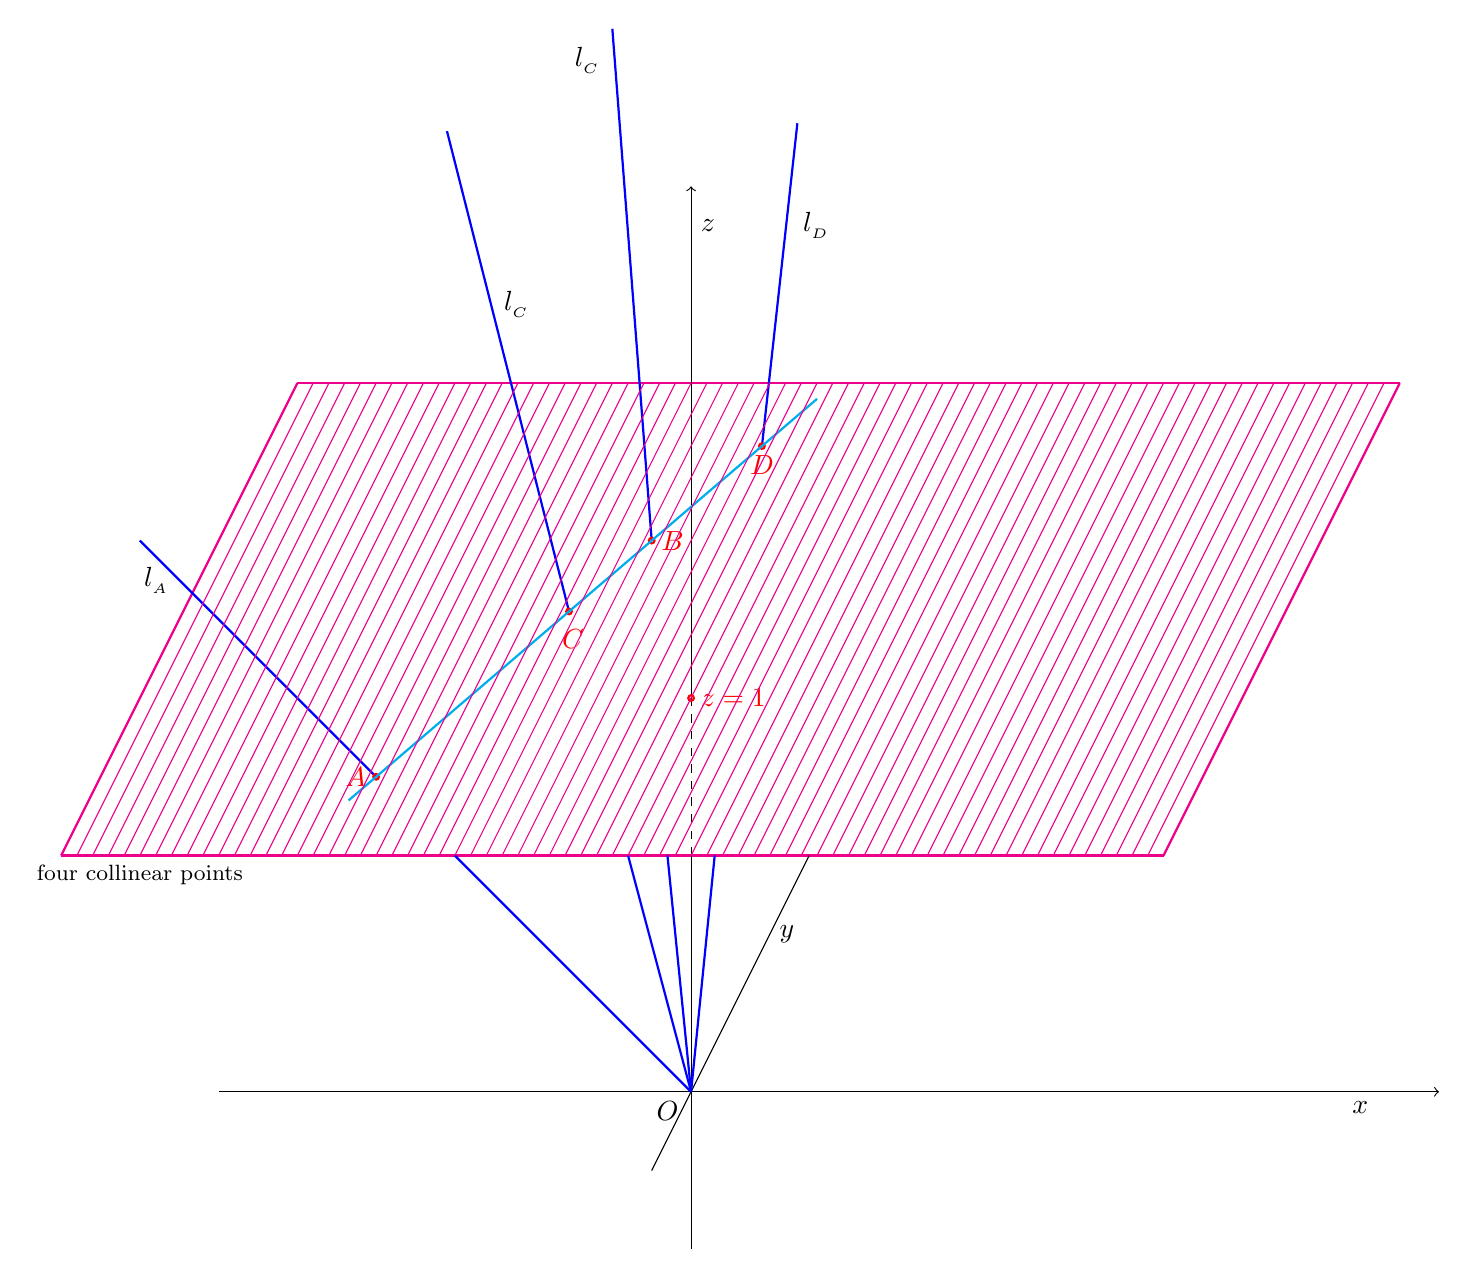
\begin{tikzpicture}
%\draw [help lines] (-10,-6) grid (6,6);

% plane $\pi$


\draw [   magenta, thick] (-10,-2)--(4,-2);
\draw [   magenta, thick] (-10,-2)--(-7,4);
\draw [   magenta, thick] (-7,4)--(7,4);
\draw [   magenta, thick] (4,-2)--(7,4);

  % origin at the point (-2,-5)
\node [below] at (-2.3,-5) {$O$};

  % Coordinate axis through the origin
\draw [ -> , thin] (-8,-5)--(7.5,-5);
\node [below] at (6.5,-5) {$x$};
\draw [  thin] (-2,-7)--(-2,-2);
\draw [  thin,dashed ] (-2,-2)--(-2,0);
\draw [ -> , thin] (-2,0)--(-2,6.5);
\node [right] at (-2,6) {$z$};
\draw [ thin] (-2.5,-6)--(-0.5,-2);
\node [right] at (-1,-3) {$y$};



% point at $z=1$, this is the point (-2,0)
\draw [red, thick] (-2,0) circle (1pt);
\node [right,red] at (-2,0) {$z=1$};

% collinear points $A,B,C, D$ at the plane

     % point A
\draw [blue, thick] (-2,-5)--(-5,-2);
\draw [blue, thick] (-6,-1)--(-9,2);
\node [left] at (-8.5,1.5) {$l_{_A}$};
\draw [red, thick] (-6,-1) circle (1pt);
\node [left,red] at (-6,-1) {$A$};

        % point C
\draw [blue, thick] (-2,-5)--(-2.8,-2);
\draw [blue, thick] (-3.55,1.1)--(-5.1,7.2);
\node [right] at (-4.5,5) {$l_{_C}$};
\draw [red, thick] (-3.55,1.1) circle (1pt);
\node [below,red] at (-3.5,1) {$C$};
      

        % point B
\draw [blue, thick] (-2,-5)--(-2.3,-2);
\draw [blue, thick] (-2.5,2)--(-3,8.5);
\node [right] at (-3.6,8.1) {$l_{_C}$};
\draw [red, thick] (-2.5,2) circle (1pt);
\node [right,red] at (-2.5,2) {$B$};

        % point D
\draw [blue, thick] (-2,-5)--(-1.7,-2);
\draw [blue, thick] (-1.1,3.2)--(-0.65,7.3);
\node [right] at (-0.7,6) {$l_{_D}$};
\draw [red, thick] (-1.1,3.2) circle (1pt);
\node [below,red] at (-1.1,3.2) {$D$};
 
% these points are at the same line:  ABCD



\draw [thick, cyan] (-6.35, -1.3)--(-0.4,3.8);

% plane $\a$ which passes through points $A,B,0)$
% vmeste s shtrikhovkoj

%\draw [thin, blue] (-2,-5)--(-4.9,-2);
%\draw [thin, blue] (-2,-5)--(-4.8,-2);
%\draw [thin, blue] (-2,-5)--(-4.7,-2);
%\draw [thin, blue] (-2,-5)--(-4.6,-2);
%\draw [thin, blue] (-2,-5)--(-4.5,-2);
%\draw [thin, blue] (-2,-5)--(-4.4,-2);
%\draw [thin, blue] (-2,-5)--(-4.3,-2);
%\draw [thin, blue] (-2,-5)--(-4.2,-2);
%\draw [thin, blue] (-2,-5)--(-4.1,-2);
%\draw [thin, blue] (-2,-5)--(-4.0,-2);
%\draw [thin, blue] (-2,-5)--(-3.9,-2);
%\draw [thin, blue] (-2,-5)--(-3.8,-2);
%\draw [thin, blue] (-2,-5)--(-3.7,-2);
%\draw [thin, blue] (-2,-5)--(-3.6,-2);
%\draw [thin, blue] (-2,-5)--(-3.5,-2);
%\draw [thin, blue] (-2,-5)--(-3.4,-2);
%\draw [thin, blue] (-2,-5)--(-3.3,-2);
%\draw [thin, blue] (-2,-5)--(-3.2,-2);
%\draw [thin, blue] (-2,-5)--(-3.1,-2);
%\draw [thin, blue] (-2,-5)--(-3.0,-2);
%\draw [thin, blue] (-2,-5)--(-2.9,-2);
%\draw [thin, blue] (-2,-5)--(-2.8,-2);
%\draw [thin, blue] (-2,-5)--(-2.7,-2);
%\draw [thin, blue] (-2,-5)--(-2.6,-2);
%\draw [thin, blue] (-2,-5)--(-2.5,-2);
%\draw [thin, blue] (-2,-5)--(-2.4,-2);
%\draw [thin, blue] (-2,-5)--(-2.3,-2);

%  shtrikhovka:

\draw [   magenta, thin] (-9.8,-2)--(-6.8,4);
\draw [   magenta, thin] (-9.6,-2)--(-6.6,4);
\draw [   magenta, thin] (-9.4,-2)--(-6.4,4);
\draw [   magenta, thin] (-9.2,-2)--(-6.2,4);
\draw [   magenta, thin] (-9.0,-2)--(-6.0,4);
\draw [   magenta, thin] (-8.8,-2)--(-5.8,4);
\draw [   magenta, thin] (-8.6,-2)--(-5.6,4);
\draw [   magenta, thin] (-8.4,-2)--(-5.4,4);
\draw [   magenta, thin] (-8.2,-2)--(-5.2,4);
\draw [   magenta, thin] (-8.0,-2)--(-5.0,4);
\draw [   magenta, thin] (-7.8,-2)--(-4.8,4);
\draw [   magenta, thin] (-7.6,-2)--(-4.6,4);
\draw [   magenta, thin] (-7.4,-2)--(-4.4,4);
\draw [   magenta, thin] (-7.2,-2)--(-4.2,4);
\draw [   magenta, thin] (-7.0,-2)--(-4.0,4);
\draw [   magenta, thin] (-6.8,-2)--(-3.8,4);
\draw [   magenta, thin] (-6.6,-2)--(-3.6,4);
\draw [   magenta, thin] (-6.4,-2)--(-3.4,4);
\draw [   magenta, thin] (-6.2,-2)--(-3.2,4);
\draw [   magenta, thin] (-6.0,-2)--(-3.0,4);
\draw [   magenta, thin] (-5.8,-2)--(-2.8,4);
\draw [   magenta, thin] (-5.6,-2)--(-2.6,4);
\draw [   magenta, thin] (-5.4,-2)--(-2.4,4);
\draw [   magenta, thin] (-5.2,-2)--(-2.2,4);
\draw [   magenta, thin] (-5.0,-2)--(-2.0,4);
\draw [   magenta, thin] (-4.8,-2)--(-1.8,4);
\draw [   magenta, thin] (-4.6,-2)--(-1.6,4);
\draw [   magenta, thin] (-4.4,-2)--(-1.4,4);
\draw [   magenta, thin] (-4.2,-2)--(-1.2,4);
\draw [   magenta, thin] (-4.0,-2)--(-1.0,4);
\draw [   magenta, thin] (-3.8,-2)--(-0.8,4);
\draw [   magenta, thin] (-3.6,-2)--(-0.6,4);
\draw [   magenta, thin] (-3.4,-2)--(-0.4,4);
\draw [   magenta, thin] (-3.2,-2)--(-0.2,4);
\draw [   magenta, thin] (-3.0,-2)--(0.0,4);
\draw [   magenta, thin] (-2.8,-2)--(0.2,4);
\draw [   magenta, thin] (-2.6,-2)--(0.4,4);
\draw [   magenta, thin] (-2.4,-2)--(0.6,4);
\draw [   magenta, thin] (-2.2,-2)--(0.8,4);
\draw [   magenta, thin] (-2.0,-2)--(1.0 ,4);
\draw [   magenta, thin] (-1.8,-2)--(1.2,4);
\draw [   magenta, thin] (-1.6,-2)--(1.4,4);
\draw [   magenta, thin] (-1.4,-2)--(1.6,4);
\draw [   magenta, thin] (-1.2,-2)--(1.8,4);
\draw [   magenta, thin] (-1.0,-2)--(2,4);
\draw [   magenta, thin] (-0.8,-2)--(2.2,4);
\draw [   magenta, thin] (-0.6,-2)--(2.4,4);
\draw [   magenta, thin] (-0.4,-2)--(2.6,4);
\draw [   magenta, thin] (-0.2,-2)--(2.8,4);
\draw [   magenta, thin] (0.0,-2)--(3.0,4);
\draw [   magenta, thin] (0.2,-2)--(3.2,4);
\draw [   magenta, thin] (0.4,-2)--(3.4,4);
\draw [   magenta, thin] (0.6,-2)--(3.6,4);
\draw [   magenta, thin] (0.8,-2)--(3.8,4);
\draw [   magenta, thin] (1.0,-2)--(4,4);
\draw [   magenta, thin] (1.2,-2)--(4.2,4);
\draw [   magenta, thin] (1.4,-2)--(4.4,4);
\draw [   magenta, thin] (1.6,-2)--(4.6,4);
\draw [   magenta, thin] (1.8,-2)--(4.8,4);
\draw [   magenta, thin] (2.0,-2)--(5,4);
\draw [   magenta, thin] (2.2,-2)--(5.2,4);
\draw [   magenta, thin] (2.4,-2)--(5.4,4);
\draw [   magenta, thin] (2.6,-2)--(5.6,4);
\draw [   magenta, thin] (2.8,-2)--(5.8,4);
\draw [   magenta, thin] (3.0,-2)--(6.0,4);
\draw [   magenta, thin] (3.2,-2)--(6.2,4);
\draw [   magenta, thin] (3.4,-2)--(6.4,4);
\draw [   magenta, thin] (3.6,-2)--(6.6,4);
\draw [   magenta, thin] (3.8,-2)--(6.8,4);


%\node [below] at (-9,-2) {${{\rm plane}\,\, z=1}$};
\node [below] at (-9,-2) {$\hbox {{\footnotesize four collinear points}}$};


\end{tikzpicture}

\begin{equation}\label{exampleoffourpointsontheline}
(A,B,C,D)={(u_A-u_C)(u_B-u_D)\over (u_A-u_D)(u_B-u_C)}\,,
\end{equation}
where $u$ an arbitrary affine coordinate.


{\bf Remark}  Cross-ratio of four points on $\R\P^2$ is well-defined
{\it only if these points are collinear.}  It is only in this case that
cross-ratio does not depend on the choice of affine coordinate.
We will assume by default that the cross-ratio is defined 
only for the collinear points. 

 
{\bf Remark} We consider here only the case if all 
these points are finite points, i.e. they have affine coordinate
\footnote{All considerations can be easily 
performed for arbitrary points.}.

{\bf Remark} Choosing an arbitrary affine coordinate
be aware that this coordinate takes different values
at these points. (See for detail solutions of exercises 3 and 4 in
Homeworks)

\m


\bigskip

{\bf Example}

Consider four points $A,B,C$ and $D$ on projective line
such that
 
$A=[8:20:4]$

$B=[8:18:2]$

$C=[6:14:2]$

$D=[t:2t+1:1]$ where $t$ is an arbitrary parameter.

First we have to check are these four points collinear, or no.
Only in the case if these four points are collinear it is meaningfull
to calculate their cross-ratio.

  Consider the affine coordinates $u={x\over z}, v={y\over z}$ 
of these points
(see equation\eqref{collinearityaffine} or  
equation\eqref{exercisethreepointsontheline} in the Example above):
                   \begin{equation}\label{secondexampleofcrossratio}
\begin{pmatrix}
    u_A\cr
    v_A\cr
\end{pmatrix}
    =
\begin{pmatrix}
    2\cr
    5\cr
\end{pmatrix}
   \,,
    \quad
\begin{pmatrix}
    u_B\cr
    v_B\cr
\end{pmatrix}
    =
\begin{pmatrix}
    4\cr
    9\cr
\end{pmatrix}
   \,,
    \quad
\begin{pmatrix}
    u_C\cr
    v_C\cr
\end{pmatrix}
    =
\begin{pmatrix}
    3\cr
    7\cr
\end{pmatrix}
   \,,
    \quad
\begin{pmatrix}
    u_D\cr
    v_D\cr
\end{pmatrix}
    =
\begin{pmatrix}
    t\cr
    2t+1\cr
\end{pmatrix}
  \,.
                   \end{equation}

We see that all these points belong to the same line
  $v=2u+1$.

\m

One can check the condition of collinearity in other way
also using  Proposition\ref{collinearity1}.

Show first that three points $A,B$ and $C$ are collinear.
Consider matrix
   $T_{ABC}=\begin{pmatrix} 
          8 & 8 & 6\cr
          20& 18 & 14\cr
          4 & 2 & 2\cr
          \end{pmatrix}
$. It is column equivalent to the matrix
$T'_{ABC}=\begin{pmatrix} 
          2 & 4 & 3\cr
          5  & 9 & 7\cr
          1 & 2 & 1\cr
          \end{pmatrix}$.

One can see that the matrix $T'_{ABC}$  is degenerate:
$\det T'_{ABC}=0$, hence the matrix $T_{ABC}$ is also degenerate.
 Hence the  points
$A,B,C$ are collinear.
In the same way one can show that three points $B,C,D$
are also collinear since 
the  matrix
   $T_{BCD}=\begin{pmatrix} 
          8 & 6 & t\cr
          18& 14 & 2t+1\cr
          2 & 2 & 1\cr
          \end{pmatrix}
$ is also degenerate.
We see that points $A,B,C$ are collinear and points
$B,C,D$ are also collinear. Hence points all four points
$A,B,C,D$ are collinear.


{\bf Remark} Sure the  first way of checking the  collinearity
of these four points 
is much shorter, than the second. 


  Niw since we also proved that these  four points are collinear,
 calculate their cross-ratio.

  Take coordinate $u$ of these points (see equation 
\eqref{secondexampleofcrossratio}). We come to
         $$
(A,B,C,D)=
{(u_A-u_C)(u_B-u_D)\over (u_A-u_D)(u_B-u_C)}=
{(2-3)(4-t)\over (2-t)(4-3)}={t-4\over 2-t\,.}
         $$
One can use another coordinate, 
   $$(A,B,C,D)=
{(v_A-v_C)(v_B-v_D)\over (v_A-v_D)(v_B-v_C)}=
{(5-7)(9-(2t+1))\over (5-(2t+1))(9-7)}={t-4\over 2-t\,.}
   $$
{\footnotesize One can use for calculation
of the cross-ration arbitrary affine coordinat
$w=au+bv+c$ which separates these points.

It is interesting to study how cross-ratio behaves
if $t\to \infty$. In accordance with equation \eqref{limitofcrossratio}
we come to
            $$
  (A,B,C,\infty)=\lim_{t\to \infty}(A,B,C,D_t)=(A,B,C)\,.
            $$
}


See other examples in Homework 9


\subsection {Conic sections and their projective 
transformations}

{\it The content of this subsection is important for general knowledge.
  This is not examinable except the analysis of 
  curve $x^2+y^2+2pxy=1$ in equation\eqref{affinetransform1}
    (see from equations \eqref{ellipsetothecircle} till equation \eqref{lastequation}.
  ) }

%\end{document}  % 8 May

In a same way as for projective line $\R\P$
one can define projective transformations of the projective plane
$\R\P^2$:
  Let $K$ be an arbitrary non-degenerate $3\times 3$
matrix
        $$
K=\begin{pmatrix} 
  a &b & c\cr
  d &e & f\cr
  g &h & k\cr
      \end{pmatrix}
\,,\quad \det K\not=0\,.
        $$ 
This matrix induces linear transformation of $\R^3$ on $\R^3$:
             \begin{equation}
  \R^3\ni 
             \begin{pmatrix}
               x\cr y\cr z\cr
                \end{pmatrix}
         \mapsto
             \begin{pmatrix}
               x'\cr y'\cr z'\cr
                \end{pmatrix}
                =\begin{pmatrix} 
  a &b & c\cr
  d &e & f\cr
  g &h & k\cr
      \end{pmatrix}
             \begin{pmatrix}
               x\cr y\cr z\cr
                \end{pmatrix}
           =
             \begin{pmatrix}
               ax+by+cz\cr 
         dx+ey+fzy\cr 
        gx+hy+kz\cr
                \end{pmatrix}\,.
            \end{equation}
 The transformation which transforms lines passing though
 origin to the lines passing through origin.   
Thus we come to transformation
$F_K$ of projective plane induced by linear transformation of $\R^3$:
\begin{equation}
F_K [x:y:z]\mapsto
    [x':y':z']=
[ax+by+cz: dx+ey+fz:gx+hy+kz]\,. 
\end{equation}
 {\footnotesize  Write down this transformation in affine coordinates.
We come to
       \begin{equation*}
u'={x'\over z'}=
{ax+by+cz\over gx+hy+kz}=
{a{x\over z}+b{y\over z}+c\over g{x\over z}+h{y\over z}+k}=
{au+bv+c\over gu+hv+k}\,,
          \end{equation*}
       \begin{equation*}
v'={y'\over z'}=
{dx+ey+fz\over gx+hy+kz}=
{d{x\over z}+e{y\over z}+f\over g{x\over z}+h{y\over z}+k}=
{du+ev+f\over gu+hv+k}\,.
          \end{equation*}

The projective transformations have an appearance of
 fractional-linear transformations
in affine coordinates.

\m

{\bf Example 1}

 Let $
K=\begin{pmatrix} 
  0 &0 & 1\cr
  d &1 & 0\cr
  1 &0 & 0\cr
      \end{pmatrix}
    $.

This matrix defines transformation
           $$
             F_K([x:y:z])=[z:y:x]\,,
            $$
i.e. in affine coordinates
$F\colon [u:v:1]\mapsto [1:u:v]=\left[{1\over v}:{u\over v}:1\right]$.

    Another example

\m

{\bf Example 2}

 Consider the transformation:
            \begin{equation}\label{geomoptics1}
                  \begin{cases}
          {1\over u'}-{1\over u}={1\over f}\cr
              {v'\over u'}={v\over u}\cr
                   \end{cases}
           \end{equation}
It is standard formula in optic. We have
 fractional linear transformation:
                         $$
                      \begin{cases}
                    u'={uf\over f+u}\cr
         v'={u'\over u}v={fv\over f+u}\cr
                              \end{cases}
                      $$
Comparing with transformation above we see that 
this transformation\footnote{One can see that transformation
\eqref{geomoptics1}
can be easily recognised as the transformation of 
geometrical optics.}  is  induced by matrix
                    $$
  K=\begin{pmatrix} 
  f &0 & 0\cr
  0 &f & 0\cr
  1 &0 & f\cr
      \end{pmatrix}
          $$


  Usual affine transforamtions of affine space are special case
of projective transformations: the matrix
 $
  K=\begin{pmatrix} 
  a &b & c\cr
  d &e & f\cr
  0 &0 & 1\cr
      \end{pmatrix}
          $  induces affine transformation
 $\begin{cases}
   u'=au+bv+c\cr
   v'=du+ev+f\cr
        \end{cases}$.
}

\bigskip

Now return to conic sections.

Recall that affine transformation,
dilation $\begin{cases}x=au\cr y=av\end{cases}$
transforms 
                     \begin{equation}\label{ellipsetothecircle}
               \hbox {an ellipse}\,\,
         {x^2\over a^2}+
         {y^2\over b^2}=1\,,\quad
        \hbox{to the circle}\,,
                u^2+v^2=1\,.
              \end{equation}

   One can consider the following
little bit more sophisticated 
 example:  Let $C$ be a curve in $\E^2$ defined
   by equation
            \begin{equation}\label{affinetransform1}
            x^2+y^2+2pxy+x+y=1\,,
                 \end{equation}
where $p$ is a parameter.

      Consider new affine coordinates  $u,v$ such that
               \begin{equation*}
               \begin{cases}
           x=u+v\cr y=u-v\cr
                  \end{cases}
          \,,\quad {\rm i.e.}\,\,
               \begin{cases}
           u={x+y\over 2}\cr v={x-y\over 2}\cr
                  \end{cases}
               \end{equation*}
This is the affine transformation, it is not
 transformations from Cartesian
coordinates to another Cartesian coordiantes
(i.e. translations and orthogonal transformations),  
 We see that in new coordinates $u,v$ curve \eqref{affinetransform1}
has appearance
                  $$
 (u+v)^2+(u-v)^2+2p(u+v)(u-v)+2u=1\Leftrightarrow
   2(1+p)u^2+2(1-p)v^2+2u=1\,.
          $$





\m 


Now analyse this curve just for
two values\footnote{ One can see that this curve is hyperbola for
$|p|>1$, it is an ellipse for $|p|<1$, for $p=-1$ 
it is parabola and for $p=1$
is the union of two parallel lines:
  $2u(u+2)-1=0
     \Rightarrow 
   u_{1,2}={-1\pm \sqrt 5\over 4}$.
}
of parameter
$p$, $p_1=-1$ and $p_2=-{1\over 2}$.

 If $p=p_1=-1$ then this curve becomes
           \begin{equation}\label{parabolaforp1}
           4v^2+2u=1\,.   
         \end{equation}
This is a parabola.


 If $p=p_2=-{1\over 2}$ then this curve becomes
           \begin{equation}\label{ellipseforp2}
           u^2+3v^2+2u=1\,.   
         \end{equation}
This is an ellipse.  Indeed
$u^2+3v^2+2u=1\Leftrightarrow
    (u+1)^2+3v^2=2\leftrightarrow
   {u'^2\over a^2}+{v'^2\over b^2}=1$,
where 
           \begin{equation}\label{lastequation}
            \begin{cases}
               u'=u-1\cr 
           v'=v\cr
             \end{cases}\,,\quad
{\rm and}\,\, a=\sqrt 2, b={\sqrt{2\over 3}}\,.
            \end{equation}



We see that changing values of parameters $p$ we come 
from parabola \eqref{parabolaforp1} to
ellipse \eqref{ellipseforp2}. 
However these  two curves cannot be transformed to each other by any affine
transformation. Does there  exist projective
transformation which transforms parabola 
\eqref{parabolaforp1} to an ellipse \eqref{ellipseforp2}?

{\footnotesize 
 To answer this question again return to the simple example
  \eqref{ellipsetothecircle}.  Consider the circle $u^2+v^2=1$
in \eqref{ellipsetothecircle} in projective plane $\R\P^2$.





Let $u,v$ be affine coordinates, and $[x:y:z]$ be homogeneous coordinates
on $\R\P^2$:
            $$
     u={x\over z}, v={y\over z}
            $$
Then the circle 
     \begin{equation*}\label{circleinaffine}
              u^2+v^2=1
                \end{equation*}
 
will have in homogeneous
coordinates the following appearance: 
             \begin{equation}\label{circleinhomogeneous}
\left(x\over z\right)^2+
\left(y\over z\right)^2=1\Leftrightarrow
      x^2+y^2=z^2\,.
                     \end{equation}
(We recall that $\left[{x\over z}:{y\over z}:1\right]=[x:y:z]$.)

onsider projective transformations  
                         \begin{equation}
F_1\colon [x:y:z]\mapsto [z:y:x]\,,   F_2\mapsto [x:y+z:y-z]\,. 
                         \end{equation}
It is easy to see that the projective transformation  $F_1$
transforms the circle \ref{circleinhomogeneous}
to hyperbola, and projective transfromation
$F_2$ transforms the circle \eqref{circleinhomogeneous}:
               $$
   F_1\colon x^2+y^2-z^2=0\mapsto z^2+y^2-x^2=0\Leftrightarrow 
           \left(x\over z\right)^2-
           \left(y\over z\right)^2=1 \Leftrightarrow u^2-v^2=1\,,
               $$    
and               $$
   F_2\colon x^2+y^2-z^2=0\mapsto x^2+(y+z)^2-(y-z)^2=0\Leftrightarrow 
         x^2+4yz=0
           \left(x\over z\right)^2+
           4\left(y\over z\right)^2=0 \Leftrightarrow u^2+4v=0\,,
               $$ 
{\it Ellipse and circle are affine equivalent, but ellipse, parabola,
and hyperbola are not affine equivalent, but they are projective equivalen.}
}
\end{document}

\centerline   {\bf Difference,Ratio and Cross-ratio. Experiment}


Let $z,A$ be an arbitary point on the line. Then one can see that the
difference
             $$
            z-A
             $$
is an invariant of translations.  
(We identify point with coordinate)

 Now consider three points $z,A,B$ then the ratio
               $$
   (z,A,B)={z-A\over z-B}
               $$
is an invariant of affine transformations:
              $$
x\mapsto ax+b\,,\quad (z,A,B) is not changed.
               $$
Now consider  for four points {\it cross-ratio}, i.e. 
ration of ratio
                 $$
   (z,u,A,B)={(z,A,B)\over (u,A,B)}={z-A\over z-B}:{u-A\over u-B}
                 $$
  Cross-ratio possesses many beautiful properties. The most important
is the following: 

  {\it it is invariant of fractional-linear transformations}
                   $$     
\mapsto {ax+b\over cx+d}\,,\quad (z,u,A,B) is not changed.
                      $$

This is an entering door in projective geometry.





